\documentclass[
% -- opções da classe memoir --
ebook,% indica que é um artigo acadêmico
extrafontsizes,
14pt,% tamanho da fonte
oneside,% para impressão apenas no recto. Oposto a twoside
a4paper,% tamanho do papel
% -- opções da classe abntex2 --
%chapter=TITLE,% títulos de capítulos convertidos em letras maiúsculas
%section=TITLE,% títulos de seções convertidos em letras maiúsculas
%subsection=TITLE,% títulos de subseções convertidos em letras maiúsculas
%subsubsection=TITLE % títulos de subsubseções convertidos em letras maiúsculas
% -- opções do pacote babel --
onecolumn,  % texto em duas colunas
english,% idioma adicional para hifenização
brazil,% o último idioma é o principal do documento
sumario=tradicional
]{abntex2}


\usepackage{dinter}


%\title{ELEMENTOS DE MATEMÁTICA APLICADA: PRINCÍPIOS, MÉTODOS E FINS}


\title{Notas de Aula} % Title

%\author{Wilson Castro Ferreira Jr}
\author{Paulo Henrique Ribeiro do Nascimento}% Author

\date{\today}% Date

\makeatletter
\let\thetitle\@title
\let\theauthor\@author
\let\thedate\@date
\makeatother

\pagestyle{fancy}
\fancyhf{}
\rhead{\theauthor}
\lhead{\thetitle}
\cfoot{\thepage}






\begin{document}
\begin{sansmath}
\helveticafamily
\def\normalfont{\helveticafamily}



%\pretextual
%\maketitle


% CAPA
%%%%%%%%%
\def\capa{
\centering
%
\includegraphics[scale = 0.75]{logo.png}\\[1.0 cm]% University Logo
\textsc{\LARGE \newline\newline Universidade Estadual de Campinas} \\[2.0 cm]% University Name
\textsc{\Large MT-624: Biomatemática I}\\[0.5 cm] % Course Code
\rule{\linewidth}{0.2 mm} \\[0.4 cm]
{ \huge \textbf{\thetitle}} \\
\rule{\linewidth}{0.2 mm} \\[1.5 cm]

\begin{minipage}{0.45\textwidth}
\begin{flushleft} \large
\emph{Professor:} \\
Wilson Castro Ferreira Jr \\
IMECC-UNICAMP \\
\end{flushleft}
\end{minipage}
\begin{minipage}{0.45\textwidth}
\begin{flushright} \large
\emph{Estudante:} \\
Paulo Henrique Ribeiro do Nascimento \\
CETEC-UFRB
\end{flushright}
\end{minipage}


\vspace{6cm}

\begin{center}
\thedate
\end{center}


\clearpage
}
%\capa




%%%%%
\tableofcontents
%\listailustracoes
%\listatabelas
%\textual
\pagebreak
%%%%%


\title{Notas de aula de Introdução ao Cálculo Fracionário}

\chapter{Funções Especiais}


\section{A Função Gama}

Partiremos de um problema para estabelecer uma relação que, com algumas manipulações, encontraremos a definição da função Gama.

Suponha que queiramos encontrar a área \(A\) da região limitada pelo gráfico da função \(f(r) = e^{-r}\), \(r \ge 0\). Dessa forma, temos
\begin{equation*}
A
= \dint_{0}^{\infty} e^{-r} \ dr
= \dlim_{b \to \infty} \dint_{0}^{b} e^{-r}\ dr
= \dlim_{b \to \infty} -e^{-r} \Bigg|_{0}^{b}
= \dlim_{b \to \infty} -e^{-b} + e^{0}
= 1,
\end{equation*}
ou seja,
\begin{equation}\label{eq:relacaoparaobtergama}
\dint_{0}^{\infty} e^{-r} \ dr = 1.
\end{equation}

Usando em \eqref{eq:relacaoparaobtergama} a substituição $r = st$, com $s>0$ (claramente $t>0$), de modo que $dr = s \ dt$, obtemos:
\begin{equation}\label{eq:relacaoparaobtergamaMV}
\dint_{0}^{\infty} e^{-st} \ dt = \dfrac{1}{s}.
\end{equation}

Derivando-se a equação\eqref{eq:relacaoparaobtergamaMV} em relação a $s$, temos:
\begin{equation}
\dint_{0}^{\infty} t e^{-st}\dt = \dfrac{1}{s^2}.
\end{equation}

Utilizando o mesmo processo:
\begin{equation}
\dint_{0}^{\infty} t^{2} e^{-st} \dt = \dfrac{2}{s^{3}}.
\end{equation}

Derivando, sucessivamente, $n$-vezes em relação a $s$:
\begin{equation}
\dint_{0}^{\infty} t^{n} e^{-st}\dt = \dfrac{n!}{s^{n+1}}.
\end{equation}

Para $s=1$, temos:
\begin{equation}
\dint_{0}^{\infty} t^{n} e^{-t}\dt = n!
\end{equation}
a relação entre do fatorial de um número inteiro \(n\) e a integral imprópria do produto do monômio de grau $n$ por uma função exponencial decrescente de base $e$.

Com o intuito de estender o conceito de fatorial de um número natural, definimos a função
\begin{equation}
g(x) = \dint_{0}^{\infty} t^{x} e^{-t} \ dt, \qquad x \in \mathbb{R} \setminus (\mathbb{Z}_{-} \cup \{1\}).
\end{equation}
Entretanto, consagrou-se a Função Gama de Euler como:
\begin{equation}
\Gamma(x) = g(x-1) = \dint_{0}^{\infty} t^{x-1} e^{-t} \ dt. \qquad x \in \mathbb{R} \setminus \mathbb{Z}_{-}
\end{equation}


Assim, a função gama completa de Euler ($\Gamma$\footnote{A notação $\Gamma$ se deve a Legendre}), ou simplesmente função gama, pode ser entendida como uma extensão da função fatorial de um número inteiro positivo para um subconjunto dos números reais ou complexos e é definida por uma integral imprópria convergente.



\subsection*{Propriedade Fundamental da Função Gama}

Comecemos por aplicar a definição para avaliar a função em $x = z+1$:
\begin{equation}
\Gamma(z+1)= \dint_{0}^{\infty} t^{z} e^{-t} \dt.
\end{equation}

Utilizando o método da integração por partes,
\begin{equation}
\Gamma(z+1)
= \left.- t^{z} e^{-t}\right\vert_{0}^{\infty}+z\dint_{0}^{\infty}t^{z-1}e^{-t}\dt
\end{equation}

Uma vez que 
$$\left.-t^{z}e^{-t}\right\vert_{0}^{\infty}=0$$
e
$$\dint_{0}^{\infty}t^{z-1}e^{-t}\dt = \Gamma(z),$$
temos,
\begin{equation}\label{propumfuncgamma}
\Gamma(z+1)=z\Gamma(z)
\end{equation}

Segue, da propriedade dada pela equação (\ref{propumfuncgamma}), que:
$$\Gamma(z+1)=z \cdot (z-1) \cdot (z-2) \cdot \ldots \cdot (z-k) \cdot \Gamma(z-k), z > k,$$
em que $k$ é um número inteiro positivo.

Observe que se $z \in \mathbb{N}$, chegaremos a $\Gamma(1) = \dint_{0}^{\infty} t^{0} e^{-t}\dt = 1$ e isso seria equivalente a calcular $z!$.

%Esta propriedade é válida também para números no domínio dos complexos.

\subsection*{Domínio da Função Gama}


Escrevendo a função Gama como:
$$\dint_{0}^{1}t^{x-1}e^{-t}\dt+\dint_{1}^{\infty}t^{x-1}e^{-t}\dt,$$
podemos ver que:
\begin{enumerate}
\item $\dint_{1}^{\infty}t^{x-1}e^{-t}\dt$ converge rapidamente, uma vez que o fator $e^{-t}$ tende a zero quando $t$ cresce indefinidamente. De outra forma, podemos usar o fato de que
$$t^{x-1} < e^{\frac{t}{2}},$$
para valores de $t$ suficientemente grandes (em outras palavras, dizemos que a função exponencial cresce mais rápido do que qualquer função polinomial). Logo, 
$$t^{x-1} e^{-t} < e^{-\frac{t}{2}}.$$

Portanto, temos que:
$$\dint_{1}^{\infty} t^{x-1} e^{-t} \dt < \dint_{1}^{\infty} e^{-\frac{t}{2}} \dt = \dfrac{2}{\sqrt{e}},$$
o que garante a convergência de $\dint_{1}^{\infty} t^{x-1} e^{-t} \dt$.

\item $\dint_{0}^{1}t^{x-1}e^{-t}\dt$, temos que a função $e^{-t}$ é limitada, para $0<t<1$. Logo, analisemos a convergência dessa integral observando o comportamento apenas do termo $t^{x-1}$.
\begin{enumerate}
\item Para $x>0$, $\dint_{0}^{1} t^{x-1}\dt= \left.\dfrac{t^{x}}{x} \right\vert_{0}^{1} = \dfrac{1}{x}<{\infty}$.
\item Para $x=0$, $\dint_{0}^{1}t^{-1}\dt={\infty}$.
\item Para $x<0$, temos que $x-1<-1$, então:
$$\dint_{0}^{1}t^{x-1}\dt>\dint_{0}^{1}t^{-1}\dt={\infty}.$$
\end{enumerate}
\end{enumerate}

Assim, a integral que define a função Gama converge, se $x>0$.


Pela propriedade fundamental, pode-se estender o domínio da função gama em intervalos que contém números negativos definindo que:
$$\Gamma(x)=\dfrac{\Gamma(x+1)}{x}.$$

Observe, aqui, que não temos uma definição para $\Gamma(x)$, com $x \in \mathbb{Z}_{-}$.

Para $x \in (-k-1, -k)$, com $k$ um número par, vê-se que $\Gamma(x) < 0$ e que
$$\dlim_{x\to -k^{-}} \Gamma(x) = \dlim_{x\to (-k-1)^{+}} \Gamma(x) = -\infty.$$

Para $x \in (-k-1, -k)$, com $k$ um número ímpar, vê-se que $\Gamma(x) > 0$ e que
$$\dlim_{x\to -k^{-}} \Gamma(x) = \dlim_{x\to (-k-1)^{+}} \Gamma(x) = \infty.$$

Dessa forma, o domínio da função Gama passa a ser $\mathbb{R} \setminus \mathbb{Z}_{-}$.

A seguir, temos o esboço do gráfico da função \(\Gamma\) no plano.


\indent

\begin{minipage}[!h]{0.9\textwidth}\centering
\psset{yunit=0.4cm,labelsep=5pt,linewidth=0.4pt,arrowsize=3pt 2,arrowinset=0.25}
\begin{pspicture*}(-5.5,-6.5)(6.2,6.2)
\psaxes[labelFontSize=\scriptstyle,Dy=2,ticksize=-2pt 0,subticks=0]{->}(0,0)(-5.5,-6)(4.5,6.5)
\multido{\iA=-1+-1}{5}{\psline[linestyle=dashed](\iA,-6)(\iA,6)}%
%\uput[d](4.6,0){$x+1$}
\psset{plotpoints=100,linewidth=1pt}
\psplot[linecolor=red]{0.01}{4}{ x GAMMA }
\psplot[linecolor=red]{-0.801}{-0.2}{ x GAMMA }
\psplot[linecolor=red]{-1.99}{-1.01}{ x GAMMA }
\psplot[linecolor=red]{-2.97}{-2.083}{ x GAMMA }
\psplot[linecolor=red]{-3.99}{-3.01}{ x GAMMA }
\psplot[linecolor=red]{-4.99}{-4.01}{ x GAMMA }

\psdots[dotsize=2pt 0,dotstyle=*](!1 1 GAMMA)\uput[90](!1 1 GAMMA){0!}
\psdots[dotsize=2pt 0,dotstyle=*](!2 2 GAMMA)\uput[90](!2 2 GAMMA){1!}
\psdots[dotsize=2pt 0,dotstyle=*](!3 3 GAMMA)\uput[110](!3 3 GAMMA){2!}
\psdots[dotsize=2pt 0,dotstyle=*](!4 4 GAMMA)\uput[200](!4 4 GAMMA){3!}
\psdots[dotsize=2pt 0,dotstyle=*](!5 5 GAMMA)\uput[200](!5 5 GAMMA){4!}
\end{pspicture*}
\end{minipage}


Utilizando as mudanças de variáveis \(t = u^{2}\) e \(v = e^{-t}\), podemos encontrar as seguintes relações para a função gama de Euler:
\begin{eqnarray}\label{funcaogama}
\Gamma(x)
&=& \dint_{0}^{\infty} t^{x-1} e^{-t} \ dt \\
&=& 2 \dint_{0}^{\infty} u^{2x-1} e^{-u^2} \ du \\
&=& \dint_{0}^{1} \left[\ln\left(\dfrac{1}{v}\right)\right]^{x-1}\ dv.
\end{eqnarray}

A função gama não possui raízes, e no campo complexo, $\Gamma$ é analítica, exceto em $\mathbb{Z}_{-}$ e o resíduo em $z=-n$ é
$$\displaystyle \mathrm{Res}_{z=-n} \Gamma(z) = \dfrac{(-1)^{n}}{n!}.$$


A função gama está relacionada:

(a) às funções gama incompletas:
$$\Gamma(a,x) = \dint_{x}^{\infty} t^{{a-1}} e^{-t}\dt.$$
$$\gamma(a,x) = \dint_{0}^{x} t^{a-1} e^{-t}\dt.$$

(b) a função digama (derivada do logaritmo da função gama):
$$\psi(x)=\dfrac{d}{\dx}\ln\left(\Gamma(x)\right) = \dfrac{\Gamma'(x)}{\Gamma(x)}.$$

São exemplos de funções ou relações que utilizam a definição da função gama:

(a) a função beta, também chamada de Integral de Euler de primeiro tipo, pode ser definida por uma razão de funções gama:
$$\beta(x,y) = \dfrac{\Gamma(x)\Gamma(y)}{\Gamma(x+y)}$$

(b) o produto entre $\Gamma(z)$ e a função zeta de Riemann $\zeta(z)$ (Havil 2003, p. 60), dada por:
$$\zeta(z)\Gamma(z)=\dint_{0}^{\infty} (u^{z-1})/(e^u-1)\du, R[z]>1.$$


% e complexos, com o argumento subtraído em $1$. Se $n$ é um inteiro positivo, define-se da seguinte forma:$$\Gamma (n+1)=n!$$
%Podemos encontrar a demonstração da convergência desta integral no artigo de Emil Artin, The Gamma Function.
%
%A função gama é debutante em diversas funções de distribuição probabilísticas, sendo assim encontra aplicações nos campos da probabilidade, estatística e combinatória.
%
%
%%Motivação
%A função gama pode ser vista como solução do seguinte problema de interpolação: Encontrar uma curva suave que conecta os pontos $(x,y)$ dados por $y = (x - 1)!$ em que $x$ é um inteiro positivo.
%
%Esboçando em um gráfico os primeiros números fatoriais fica claro que a curva pode ser desenhada, mas seria preferível ter um expressão analítica que descreve precisamente a curva, na qual o número de operações não dependa do tamanho de x. A simples fórmula recursiva para o fatorial x! = x \times ... \times 2 \times 1, não pode ser usada para obter valores fracionários, pois é válida apenas quando x é um número natural. No entanto, foi demonstrado por Euler que não há uma expressão analítica convencional para fatorial, no sentido que não pode ser a combinação finita (com um número finito de termos) de somas, potências, produtos, funções exponenciais e logaritmos, demonstrado em seu artigo intitulado "Sobre progressões transcendentais, nas quais o termo geral não pode ser expresso algebricamente", ("De progressionibus transcendentibus seu quarum termini generales algebraice dari nequeunt"). A função gama é uma solução que não só resolve este problema, mas também possuí distinguíveis propriedades entre as candidatas, como é mostrado no Teorema de Bohr-Mollerup.
%
%Prova[editar | editar código-fonte]



Em suma, vale lembrar que a função gama aparece ocasionalmente em diversos problemas físicos tais como a normalização das funções de onda de Coulomb e o computo de probabilidades em mecânica estatística, embora sua importância, na verdade, é derivada de sua utilidade no desenvolvimento de outras funções que apresentam aplicações físicas diretas, como a de Bessel. Além desta definição em termos de integral imprópria, devida a Euler, temos no mínimo outras duas definições equivalentes da função gama, uma através de um limite infinito (também devida a Euler) e outra através de um produto infinito (devida a Weierstrass) (ver, por exemplo, Arfken [4]).

Muito da importância da função gama provem da seguinte fórmula facilmente demonstrável
usando-se integração por partes,
$$\Gamma(p+1) = p\Gamma(p).$$
Daí resulta que, quando $p = n$ é um inteiro não-negativo,
$$\Gamma(n+1) = n!$$
de maneira que a função gama generaliza o fatorial de números inteiros positivos para valores reais. A figura seguinte mostra o gráfico da função gama.




\subsection*{Alguns resultados notáveis}

\exemplo{}{
Prove que o zero fatorial é igual a um.
}

\solexemplo{
Temos que:
\[\Gamma(1)=0!=\dint_{0}^{\infty} t^{1-1} e^{-t}\dt = \left.-e^{-t} \right\vert_{0}^{\infty} = 1.\]
}


\exemplo{}{
Determine o valor $\Gamma\left(\dfrac{1}{2}\right)$.
}

\solexemplo{
\[\Gamma\left(\dfrac{1}{2}\right) =\dint_{0}^{\infty} t^{-\frac{1}{2}} e^{-t}\dt.\]

Fazendo $t=r^{2}$, obtemos $\dt=2r\dr$.

Logo,
\[\dint_{0}^{\infty}t^{-\frac{1}{2}} e^{-t}\dt = 2 \dint_{0}^{\infty}e^{-r^{2}}\dr.\]

Utilizando a técnica de Liouville, temos que:
\[I = \dint_{0}^{\infty} e^{-x^{2}}\dx = \dint_{0}^{\infty} e^{-y^{2}}\dy.\]

Logo, podemos escrever
\[I^{2}=\dint_{0}^{\infty} e^{-x^{2}} \dx \dint_{0}^{\infty} e^{-y^{2}}\dy = \dint_{0}^{\infty}\dint_{0}^{\infty} e^{-(x^{2}+y^{2})} \dx\dy.\]

Fazendo a mudança de variáveis em coordenadas polares:
\[I^{2}=\dint_{0}^{\frac{\pi}{2}}\dint_{0}^{\infty} e^{-r^{2}}r\dr\dtheta = \dfrac{\pi}{4}.\]

Como
\[I=\frac{\sqrt{\pi}}{2},\]
temos que
\[2\dint_{0}^{\infty}e^{-r^{2}}\dr = 2 \dfrac{\sqrt{\pi}}{2} = \sqrt{\pi}.\]

Sendo assim:
\[\Gamma\left(\dfrac{1}{2}\right)=\sqrt{\pi}.\]
}


%Referências
%
%Boyce e DiPrima. Equações Diferenciais Elementares e Problemas de Valores de Contorno, editora LTC, 9ª edição, 2010.
%Dennis G. Zill, Michael R. Cullen; Equações Diferenciais, vol 1; Editora Makron Books do Brasil;
%Davis, Philip J.; Abramowitz, Milton; Stegun, Irene. Handbook of Mathematical Functions with Formulas, Graphs, and Mathematical Tables. 1972.



\section{A Função Beta}


\definicao{}{}{
A função \(\mathfrak{B}(y,x)\), também chamada de integral de Euler de primeiro tipo, é definida por
\begin{equation}\label{eq:beta}
\displaystyle \mathfrak{B}(y,x) = \int_{0}^{1} t^{x-1}\ (1-t)^{y-1}\ dt
\end{equation}
}



\subsection{Propriedades}

\proposicao{}{}{
A função beta é simétrica, o que significa que:
\begin{equation}
\mathfrak{B}(y,x) = \mathfrak{B}(x,y).
\end{equation}
}

\textbf{Demonstração}:

Tomando \(u = 1-t \Rightarrow du = -dt\). Segue que
\[\begin{array}{rcl}
\mathfrak{B}(y,x)
&=& \displaystyle\int_{0}^{1} t^{x-1}\ (1-t)^{y-1}\ dt \\
&=& \displaystyle\int_{1}^{0} (1-u)^{x-1}\ u^{y-1}\ -du \\
&=& \displaystyle\int_{0}^{1} (1-u)^{x-1}\ u^{y-1}\ du \\
&=& \mathfrak{B}(x,y).
\end{array}\]



\subsection{Outras formas da função beta}


\proposicao{}{}{
A função beta possui a forma trigonométrica:
\begin{equation}
\displaystyle \mathfrak{B}(y,x) = 2 \int_{0}^{\frac{\pi}{2}} [\cos(\theta)]^{2x-1}[\sin(\theta)]^{2y-1}\,\mathrm{d}\theta,\qquad \mathrm{Re}(x) > 0,\ \mathrm{Re}(y) > 0.
\end{equation}
}

\textbf{Demonstração}: Apliquemos a mudança de variáveis \(t = \cos^2(\theta) \Rightarrow dt = -2\cos(\theta)\sin(\theta) d\theta\) em \eqref{eq:beta}. Assim,
\[\begin{array}{rcl}
\mathfrak{B}(y,x)
&=& \displaystyle\int_{\frac{\pi}{2}}^{0} [\cos^2(\theta)]^{x-1}\ [1-\cos^2(\theta)]^{y-1} [-2\cos(\theta)\sin(\theta)]\ d\theta \\
&=& \displaystyle\int_{0}^{\frac{\pi}{2}} [\cos(\theta)]^{2x-2}\ [\sin(\theta)]^{2y-2} [2\cos(\theta)\sin(\theta)]\ d\theta \\
&=& 2 \displaystyle\int_{0}^{\frac{\pi}{2}} [\cos(\theta)]^{2x-1}\ [\sin(\theta)]^{2y-1}\ d\theta.
\end{array}\]



\proposicao{}{}{
A expressão de beta em função de \(\Gamma\) é:
\begin{equation}
\displaystyle \mathfrak{B}(y,x) = \dfrac{\Gamma(x)\,\Gamma(y)}{\Gamma(x+y)}.
\end{equation}
}


\textbf{Demonstração}: Temos que
\[\begin{array}{rcl}
\Gamma(x) &=& \displaystyle\int_{0}^{\infty} e^{-t} t^{x-1}\ dt \\
\Gamma(y) &=& \displaystyle\int_{0}^{\infty} e^{-s} s^{y-1}\ ds \\
\end{array}\]


Apliquemos as seguintes mudanças de variáveis:
\[\begin{array}{rcl}
t = u^2 &\Rightarrow& dt = 2u\,du \\
s = v^2 &\Rightarrow& ds = 2v\,dv
\end{array}\]

Então,
\[\begin{array}{rcl}
\Gamma(x)
&=& \displaystyle\int_{0}^{\infty} e^{-u^2} u^{2x-2}\ 2u\,du
= 2 \int_{0}^{\infty} e^{-u^2} u^{2x-1}\,du \\
\Gamma(y)
&=& \displaystyle\int_{0}^{\infty} e^{-v^2} v^{2y-2}\ 2v\,dv
= 2 \int_{0}^{\infty} e^{-v^2} v^{2y-1}\,dv \\
\end{array}\]

Logo,
\[
\Gamma(x)\cdot\Gamma(y) = 4 \displaystyle\int_{0}^{\infty}\int_{0}^{\infty} e^{-(u^2+v^2)} u^{2x-1} v^{2y-1} \ du\ dv
\]

Apliquemos, agora, as seguintes mudanças de variáveis:
\[\begin{array}{rcl}
u = r\cos(\theta) \\
v = r \sin(\theta)
\end{array}\]

Segue que
\[\begin{array}{rcl}
\Gamma(x)\cdot\Gamma(y)
&=& 4 \displaystyle\int_{0}^{\frac{\pi}{2}}\int_{0}^{\infty} e^{-r^2} r^{2x-1} [\cos(\theta)]^{2x-1} r^{2y-1} [\sin(\theta)]^{2y-1}\ r\ dr\ d\theta \\
&=& 4 \displaystyle\int_{0}^{\frac{\pi}{2}}\int_{0}^{\infty} e^{-r^2} r^{2x+2y-1} [\cos(\theta)]^{2x-1} [\sin(\theta)]^{2y-1}\ dr\ d\theta \\
&=& \underbrace{2\displaystyle\int_{0}^{\infty} e^{-r^2} r^{2x+2y-1} \dr}_{k} \cdot \underbrace{2\int_{0}^{\frac{\pi}{2}} [\cos(\theta)]^{2x-1} [\sin(\theta)]^{2y-1}\ d\theta}_{\mathfrak{B}(y,x)}
\end{array}\]

Para determinarmos \(I\), façamos a seguinte mudança de variável
\[r^2 = \xi \Rightarrow 2r\ dr = d\xi.\]

Portanto,
\[I = \displaystyle\int_{0}^{\infty} e^{-\xi} \xi^{y+x-1}\ d\xi = \Gamma(y+x)\]

Segue que
\[\Gamma(y) \cdot \Gamma(x) = \Gamma(y+x) \mathfrak{B}(y,x).\]

\begin{corollary}
Se \(x\) e \(y\) são inteiros positivos, então:
\begin{equation}
\displaystyle \mathfrak{B}(x,y) = \dfrac{(x-1)!\,(y-1)!}{(x+y-1)!}.
\end{equation}
\end{corollary}



\proposicao{}{}{
A expressão de beta assume as formas:
\begin{eqnarray}
\displaystyle \mathfrak{B}(x,y) &=& \int_{0}^{\infty} \dfrac{t^{x-1}}{(1+t)^{x+y}}\,\mathrm{d}t,\qquad \mathrm{Re}(x) > 0,\ \mathrm{Re}(y) > 0. \\
\displaystyle \mathfrak{B}(x,y) &=& \sum_{n=0}^{\infty} \dfrac{\binom{n-y}{n}}{x+n}. \\
\displaystyle \mathfrak{B}(x,y) &=& {\dfrac{x+y}{xy}} \prod_{n=1}^{\infty} \left(1+{\dfrac{xy}{n(x+y+n)}}\right)^{-1}.
\end{eqnarray}
}

\subsection{Algumas Identidades}

\proposicao{}{}{
A função Beta satisfaz as identidades
\begin{eqnarray}
\displaystyle \mathfrak{B}(x,y) &=& \mathfrak{B}(x,y+1)+\mathfrak{B}(x+1,y) \\
\displaystyle \mathfrak{B}(x+1,y) &=& \mathfrak{B}(x,y) \cdot \dfrac{x}{x+y} \\
\displaystyle \mathfrak{B}(x,y+1) &=& \mathfrak{B}(x,y)\cdot \dfrac{y}{x+y} \\
\displaystyle \mathfrak{B}(x,y) \cdot (t \mapsto t_{+}^{x+y-1}) &=& (t \to t_{+}^{x-1})*(t\to t_{+}^{y-1})\qquad x\geq 1,y\geq 1 \\
\displaystyle \mathfrak{B}(x,y)\cdot \mathfrak{B}(x+y,1-y) &=& \dfrac{\pi}{x\sin(\pi y)}\label{eq:identidade5},
\end{eqnarray}
onde \(\displaystyle t\mapsto t_{+}^{x}\) é um função de potência truncada e a estrela da denota convolução.
}

\textbf{Observações}:

\begin{enumerate}
\item A identidade\eqref{eq:identidade5} demonstra, em particular, que \(\displaystyle \Gamma\left(\dfrac{1}{2}\right) = \sqrt{\pi}\).

\item Algumas destas identidades, por exemplo, a fórmula trigonométrica, pode ser aplicada para derivar o volume de uma bola-n[3][4][5] em coordenadas cartesianas.

\item A integral de Euler para a função Beta pode ser convertida em uma integral sobre o contorno \(C\) de Pochhammer [6] [7] [8] como:
\begin{equation}
\displaystyle \displaystyle (1-e^{2\pi i\alpha})(1-e^{2\pi i\beta})\mathfrak{B}(\alpha ,\beta) = \int_{C} t^{\alpha-1}(1-t)^{\beta-1}\, \mathrm{d} t.
\end{equation}

Esta integral do contorno de Pochhammer converge para todos os valores de \(\alpha\) e \(\beta\) e assim dá a continuação analítica da função beta.

\item Assim como a função gama ``\(\Gamma\)'' para inteiros descreve fatoriais, a função beta pode definir um coeficiente binomial depois de ajustar os índices:
\[\displaystyle \binom{n}{k} = \dfrac{1}{(n+1) \mathfrak{B}(n-k+1,k+1)}.\]
Além disso, para o inteiro \(n\), \(\displaystyle \mathfrak{B}\) pode ser fatorado para dar uma forma fechada, uma função de interpolação para valores contínuos de \(k\):
\begin{equation}
\displaystyle \binom{n}{k} = (-1)^{n}n! {\cfrac{\sin(\pi k)}{\pi \displaystyle \prod_{i=0}^{n}(k-i)}}.
\end{equation}

\item A função beta foi a primeira amplitude de dispersão conhecida na teoria das cordas, primeiramente conjecturado por Gabriele Veneziano. Ocorre também na teoria do processo de ligação preferencial [9] [10], um tipo de processo de urna [11] estocástica.
\end{enumerate}

\subsection{Função beta incompleta}

\definicao{}{}{
A função beta incompleta (generalização da função beta) é dada por:
\begin{equation}
\mathfrak{B}(\tau;\, y,x) = \displaystyle \int_{0}^{\tau} t^{x-1}\,(1-t)^{y-1}\,dt.
\end{equation}
}

Para \(\tau = 1\), a função beta incompleta coincide com a função beta completa, ou seja,
\[\mathfrak{B}(1;\, y,x) = \mathfrak{B}(y,x)\]

\textbf{Observação}: A relação existente entre estas duas funções é como a que existe entre a função gama e sua generalização, a função gama incompleta.

\definicao{}{}{
A função beta incompleta regularizada (ou função beta regularizada para abreviar) é definida em termos da função beta incompleta e da função beta completa por:
\begin{equation}
\mathfrak{B}_{\tau}(y,x) = \dfrac{\mathfrak{B}(\tau;\,y,x)}{\mathfrak{B}(y,x)}.
\end{equation}
}




\section{Funções de Mittag-Leffler}

\subsection{Funções de Mittag-Leffler com um parâmetro}

\definicao{}{}{
A função de Mittag-Leffler com UM parâmetro \(\alpha \in \mathbb{C}, \ \mathrm{Re}(\alpha) > 0\) é dada por:
\begin{equation}
\mathfrak{E}_\alpha = \displaystyle\sum_{k=0}^{\infty} \dfrac{t^k}{\Gamma(\alpha k + 1)}, \ \mathrm{Re}(\alpha) > 0.
\end{equation}
}

\textbf{Observação}:
\begin{equation}
\mathfrak{E}_1 = \displaystyle\sum_{k=0}^{\infty} \dfrac{t^k}{\Gamma(k + 1)} = \displaystyle\sum_{k=0}^{\infty} \dfrac{t^k}{k!} = e^t.
\end{equation}

\subsection{Funções de Mittag-Leffler com dois parâmetros}

\definicao{}{}{
A função de Mittag-Leffler com DOIS parâmetros é dada por:
\begin{equation}
\mathfrak{E}_{\alpha,\beta} = \displaystyle\sum_{k=0}^{\infty} \dfrac{t^k}{\Gamma(\alpha k + \beta)}.
\end{equation}
}



\subsection{Valores notáveis}

\proposicao{}{}{
\begin{eqnarray}
\label{eq:mittagalphaum}
\mathfrak{E}_{\alpha,1}(z)
&=& \mathfrak{E}_{\alpha}(z). \\
%
\label{eq:mittagumum}
\mathfrak{E}_{1,1}
&=& e^z. \\
%
\label{eq:mittagzeroum}
\mathfrak{E}_{0,1}
&=& \dfrac{1}{1-z},\qquad |z| < 1.
\end{eqnarray}
}



\proposicao{}{}{
\begin{eqnarray}
\mathfrak{E}_{1,n}(z)
= \dfrac{1}{z^{n-1}} \left[e^z + \displaystyle\sum_{k=0}^{n-2} z^k\right].
\end{eqnarray}
}


\begin{eqnarray}
\label{eq:mittagumdois}
\mathfrak{E}_{1,2}(z)
&=& \displaystyle\sum_{k=0}^{\infty} \frac{z^k}{\Gamma(k+2)}
= \displaystyle\sum_{k=0}^{\infty} \frac{z^k}{(k+1)!}
= \frac{1}{z} \displaystyle\sum_{k=0}^{\infty} \frac{z^{k+1}}{(k+1)!} \\
\nonumber
&=& \frac{1}{z} \left(-1+1+z+\frac{z^2}{2!}+\frac{z^3}{3!}+\ldots\right)
= \frac{-1+e^z}{z}. \\
%
\label{eq:mittagumtres}
\mathfrak{E}_{1,3}(z)
&=& \displaystyle\sum_{k=0}^{\infty} \frac{z^k}{\Gamma(k+3)}
= \displaystyle\sum_{k=0}^{\infty} \frac{z^k}{(k+2)!}
= \frac{1}{z^2} \displaystyle\sum_{k=0}^{\infty} \frac{z^{k+2}}{(k+2)!} \\
\nonumber
&=& \frac{1}{z^2} \left(-1-z+1+z+\frac{z^2}{2!}+\frac{z^3}{3!}+\ldots\right)
= \frac{-1-z+e^z}{z^2}. \\
&\vdots&
\end{eqnarray}



\proposicao{}{}{
\begin{eqnarray}
\mathfrak{E}_{2,1}(z) &=& \cosh(\sqrt{z}) \\
\mathfrak{E}_{2,2}(z^2) &=& \dfrac{1}{z}\sinh(\sqrt{z}) \\
\mathfrak{E}_{2,1}(-z^2) &=& \cos(z) \\
\mathfrak{E}_{2,2}(-z^2) &=& \dfrac{1}{z}\sin(z)
\end{eqnarray}
}

\subsection{Relação de recorrência da Função de Mittag Leffer}

\proposicao{}{}{
\begin{eqnarray}
\mathfrak{E}_{\alpha,\beta}(Z) = z \mathfrak{E}_{\alpha,\alpha+\beta}(Z) + \dfrac{1}{\Gamma(\beta)}
\end{eqnarray}
}






\subsection{Transformada de Laplace da função de Mittag-Leffler}

\definicao{}{}{
Seja \(f\) uma função contínua por partes
\begin{equation}
F(s) = \mathcal{L}\{f(t)\} = \displaystyle\int_{0}^{\infty} e^{-st}\ f(t)\ dt,
\end{equation}
onde \(f\) é 
}


%MT952-AULA00–Introdução ao Cálculo Fracionário

\chapter{Sobre algumas integrais}

Como é sabido, várias integrais reais são de difícil resolução. Muitas vezes, sempre que possível, fazemos uso do plano complexo para calcular as integrais reais. Além disso, vários truques são sempre sugeridos, dentre eles aquele que atende pelo nome de integrais de Feynman.

Como uma breve introdução, vamos discutir duas integrais aparentemente complicadas que com um pouco de treino são reduzidas a integrais de fácil manipulação. Imediatamente após apresentamos o truque proposto por Feynman para calcular integrais reais.

\section{Substituição trigonométrica}

Através de dois exemplos, utilizando substituição trigonométrica, vamos calcular duas integrais reais, aparentemente não imediatas.

\exemplo{exam:01}{
%Exemplo 1.
Seja $x \in \mathbb{R}$. Calcular a integral
$$\Lambda = \dint \sin(2 \arctan(x)) dx.$$
}

\solexemplo{Começamos com a relação trigonométrica envolvendo o seno do arco dobro, assim
$$\Lambda = 2 \dint \sin(\arctan(x)) \cos(\arctan(x)) dx.$$

Agora, introduzimos a mudança de variável $\arctan(x) = u$, de onde segue, $\tan(u) = x$ e $dx = \sec^{2}(u) du$. Logo,
$$\Lambda = 2 \dint \sin(u) \cos(u) \sec^{2}(u) du,$$
ou ainda, na seguinte forma,
$$\Lambda = 2 \dint \dfrac{\sin(u)}{\cos(u)} du.$$

Essa integral é calculada a partir da mudança de variável $\cos(u) = t$ cujo diferencial é exatamente o numerador, de
onde podemos escrever
$$\Lambda = 2 \dint -\dfrac{1}{t} dt = -2 \dint \dfrac{1}{t} dt$$
que é uma integral imediata
$$\Lambda = -2 \ln|t| + C,$$
onde $C$ é uma constante de integração.

Voltando com as variáveis que foram introduzidas a partir das mudanças de variáveis, obtemos
$$\Lambda = \ln(1 + x^{2}) + C$$
sendo $C$ uma constante de integração.

Vamos, agora, obter o mesmo resultado através de uma simplificação que, sempre que possível, agiliza o cálculo.

Considere o triângulo retângulo:
\begin{center}
\captionof{figure}{\small Triângulo retângulo: seno, cosseno e tangente.}
\label{fig:01}
\begin{pspicture}(-.5,-.5)(4.5,4.5)
\pnode(4,0){A}
\pnode(4,3){B}
\pnode(0,0){C}
\pspolygon(A)(B)(C)
\rput(0,.5){\rput{36.87}(2.2;36.87){$\sqrt{1+x^2}$}}
\uput[r](4,1.5){$x$}
\uput[d](2,0){$1$}
\psarc{-}(0,0){0.9}{0}{36.87}
\rput(1.1;18.44){$u$}
\end{pspicture}
\end{center}

Da \autoref{fig:01} são imediatas as relações
$$\tan(u) = x, \sin(u) = \dfrac{x}{\sqrt{1 + x^{2}}}, \cos(u) = \dfrac{1}{\sqrt{1 + x^{2}}}.$$

Assim, substituindo na integral de partida, temos:
$$
\Lambda
= 2 \dint \dfrac{x}{\sqrt{1 + x^{2}}} \dfrac{1}{\sqrt{1 + x^{2}}} dx
= 2 \dint \dfrac{x}{1 + x^{2}} dx
= \ln(1+x^2) + C,
$$
que é o resultado desejado.
}



\exercicio{}{%Do lar 1.
Complete a integração e obtenha o mesmo resultado, conforme metodologia anterior.
}

\solexercicio{Aqui, basta tomar $x = \tan(t)$. Segue que, $dx = \sec^{2}(t) dt$.

Logo,
$$\Lambda = 2 \int \dfrac{\sin(t)}{\cos(t)} dt = 2\ln|\sec(t)| + C$$
}



\exemplo{exam:02}{
%Exemplo 2.
Seja $x \in \mathbb{R}$. Calcular a integral
$$\Omega = \dint \dfrac{dx}{2 + \cos(x)}.$$
}

\solexemplo{Observemos que o denominador nunca se anula (a integral é não singular). 

Vamos introduzir a mudança de variável envolvendo a tangente do arco metade. 

Analogamente à integral discutida no Exemplo \ref{exam:01}, considere o triângulo retângulo:
\begin{center}
\captionof{figure}{\small Triângulo retângulo: seno, cosseno e tangente do arco metade.}
\label{fig:02}
\begin{pspicture}(-.5,-.5)(4.5,4.5)
\pnode(4,0){A}
\pnode(4,3){B}
\pnode(0,0){C}
\pspolygon(A)(B)(C)
\rput(0,.5){\rput{36.87}(2.2;36.87){$\sqrt{1+t^{2}}$}}
\uput[r](4,1.5){$t$}
\uput[d](2,0){$1$}
\psarc{-}(0,0){0.9}{0}{36.87}
\rput(1.1;18.44){$\frac{x}{2}$}
\end{pspicture}
\end{center}

Da \autoref{fig:02} seguem as relações
$$\tan\left(\dfrac{x}{2}\right) = t, \sin\left(\dfrac{x}{2}\right) = \dfrac{t}{\sqrt{1 + t^{2}}} \mbox{ e } \cos\left(\dfrac{x}{2}\right) = \dfrac{1}{\sqrt{1 + t^{2}}}.$$


Utilizando a expressão para o cosseno do arco dobro, podemos escrever
$$\cos(x)
=
\left(\dfrac{1}{\sqrt{1 + t^{2}}}\right)^{2}
- \left(\dfrac{t}{\sqrt{1 + t^{2}}}\right)^{2}
=
\dfrac{1 - t^{2}}{1 + t^{2}}.$$

Ainda mais, para o diferencial, temos:
$$dt = \dfrac{1}{2} \sec^{2} \left(\dfrac{x}{2}\right) dx \Rightarrow dx = \dfrac{2 dt}{1 + t^{2}}.$$

Substituindo na integral a ser calculada e simplificando, obtemos a seguinte integral:
$$\Omega
=
\dint
\dfrac{2 dt}{1 + t^{2}}
\left(\dfrac{1}{2 + \dfrac{1-t^{2}}{1 + t^{2}}}\right)
= 2 \dint \dfrac{dt}{t^{2} + 3}.$$

Esta integral é tabelada. Logo,
$$\Omega
= \dfrac{2}{\sqrt{3}} \arctan\left(\dfrac{t}{\sqrt{3}}\right)
+ C,$$
em que $C$ é uma constante de integração.

Voltando com a mudança de variável, obtemos:
$$
\Omega = \dfrac{2}{\sqrt{3}} \arctan\left[\dfrac{1}{\sqrt{3}} \tan\left(\dfrac{x}{2}\right)\right] + C,
$$
sendo $C$ a constante de integração.
}



\section{Metodologia de Feynman}

Este truque, popularizado por Feynman, visando o cálculo de integrais reais, está baseado na possibilidade de se poder derivar sob o sinal de integral.

\subsection{Derivação sob o sinal de integral}


Considere $D \subset \mathbb{R}^{2}$ e $f: D \to \mathbb{R}$, uma função de classe $C^{1}$ em $D$ e o retângulo $[a, b] \times [c, d] \subset D$.

Seja a função
$F: [c, d] \to \mathbb{R}$, tal que
\begin{equation}
\label{eq:01}
F(\alpha) = \dint_{a}^{b} f(x, \alpha) dx.
\end{equation}
Logo $F(\alpha)$ é uma integral dependendo do parâmetro $\alpha$.

\teorema{}{}{\label{teo:01}
%Teorema 1.
A derivada em relação ao parâmetro $\alpha$
comuta com a integração em relação à variável $x$, ou seja,
$$
\dfrac{d}{d\alpha} \dint_{a}^{b} f(x, \alpha) dx
=
\dint_{a}^{b} \dfrac{\partial}{\partial \alpha} f(x, \alpha) dx.$$
}

\demteorema{Ver \cite{deoliveira2021}. %\footnote{oliveira@ime.usp.br}, \href{http://www.ime.usp.br/\%7Eoliveira}{http://www.ime.usp.br/$\sim$oliveira}.
}

Voltemos ao método. Vamos subdividir em quatro etapas para padronizar a metodologia.

Considere o problema de calcular a integral
\begin{equation}\label{eq:integraldefx}
\displaystyle\int_{a}^{b} f(x) dx.
\end{equation}
O método consiste em:
\begin{enumerate}
\item Introduzindo um parâmetro $\alpha$ no integrando de \eqref{eq:integraldefx}, transformando-o em $f(x,\alpha)$, criando, assim uma função
\begin{equation}\label{eq:funcaoFalpha}
F(\alpha) = \displaystyle\int_{a}^{b} f(x, \alpha) dx,
\end{equation}
de forma conveniente.
\item Após diferenciamos \eqref{eq:funcaoFalpha} com respeito ao parâmetro \(\alpha\), ou seja, determinarmos uma expressão para $\dfrac{d}{d\alpha} F(\alpha)$, efetuando a integração em relação a $x$, obtemos uma equação diferencial.

\item Resolvemos a equação diferencial para obter uma expressão para $F(\alpha)$. Note que $F(\alpha)$ não deve ser função da variável de integração.

\item Com o conveniente valor de $\alpha$, obter a integral de partida.
\end{enumerate}

É importante notar que a dificuldade reside na primeira etapa, pois a partir da segunda, é calcular uma derivada, resolver uma equação diferencial e calcular o valor de uma função num ponto ou substituir o valor do parâmetro por um número conveniente. Ainda mais, ao introduzir o parâmetro ou a função, coisa que requer treino e mais treino além, claro, de criatividade, devemos ser capazes de integrar. Vamos apresentar o cálculo explícito para alguns exemplos.

\exemplo{exam:03}{
%Exemplo 3.
Seja $x \in \mathbb{R}$. Calcule a integral
$$\mathcal{I} = \dint_{0}^{\infty} \dfrac{\sin(x)}{x} dx,$$
conhecida como a integral de Dirichlet.
}

\solexemplo{Apenas para mencionar, esta integral é um clássico exemplo que faz uso plano complexo para calcular uma integral real. Vamos utilizar o truque de Feynman.

Esta é uma integral que não é absolutamente convergente, logo não está definida no sentido da integração de Lebesgue. Ainda mais, esta é uma integral clássica que é calculada através do plano complexo, como já mencionamos. Em particular, o integrando $f(z) = \dfrac{\sin(z)}{z}$ é uma função que apresenta uma singularidade removível; com um contorno evitando o zero do denominador.

Aqui, a fim de utilizar a metodologia de Feynman, introduzimos uma função $e^{\alpha x}$, com $\alpha \leq 0$\footnote{A importância de impormos o parâmetro não estritamente positivo é devido ao extremo superior da integral de partida.}, tal que
$$F(\alpha) = \dint_{0}^{\infty} \dfrac{\sin(x)}{x} e^{\alpha x} dx.$$

Com esta função, recuperamos a integral inicial a partir de $\alpha = 0$, de onde obtemos $F(0) = \mathcal{I}$.

Agora, derivamos a função em relação ao parâmetro $\alpha$ (derivada parcial, pois o integrando é uma função de duas variáveis)
$$\dfrac{d}{d\alpha} F(\alpha)
=
\dint_{0}^{\infty} \dfrac{\sin(x)}{x} x e^{\alpha x} dx
=
\dint_{0}^{\infty} \sin(x) e^{\alpha x} dx$$

A fim de resolver esta integral, podemos utilizar duas vezes integração por partes, porém, aqui, vamos usar a
relação de Euler
$$\sin(x) = \dfrac{1}{2i} (e^{ix} - e^{-ix})$$
de onde podemos escrever, apenas para o segundo membro, denotado por $\mathbb{I}_M$,
$$
\mathbb{I}_M =
\dfrac{1}{2i}
\dint_{0}^{\infty}
(e^{ix} - e^{-ix}) e^{\alpha x} dx
=
\dfrac{1}{2i}
\dint_{0}^{\infty}
[e^{x(\alpha +i)} - e^{x(\alpha -i)}] dx.
$$

Note que as integrais existem, pois com a imposição no parâmetro $a$, convergem. Logo, integrando e simplificando, temos:
$$
\mathbb{I}_M =
\dfrac{1}{2i}
\left[
\dfrac{e^{x(\alpha+i)}}{\alpha+i} - \dfrac{e^{x(\alpha-i)}}{\alpha-i}
\right]_{x=0}^{\infty}
=
\dfrac{1}{2i}
\left(-\dfrac{1}{\alpha+i} + \dfrac{1}{\alpha-i}\right)
=
\dfrac{1}{1+\alpha^{2}}.
$$

Assim, voltando na expressão para a derivada, obtemos:
$$\dfrac{\partial }{\partial \alpha} F(\alpha) = \dfrac{1}{1+\alpha^{2}}$$
que é uma equação diferencial cuja integração é imediata, pois é a primitiva do arco tangente. Logo,
$$F(\alpha) = \arctan(\alpha) + C,$$
onde $C$ é uma constante de integração.

A próxima etapa requer determinar a constante de integração. Para tal, aqui, vamos considerar o limite do parâmetro $\alpha \to -\infty$. Logo
$$\displaystyle\lim_{\alpha\to-\infty} F(\alpha) = \lim_{\alpha\to-\infty} (\arctan(\alpha) + C) = -\dfrac{\pi}{2} + C$$
que, levando na definição de $F(\alpha)$ fornece
$$-\dfrac{\pi}{2} + C = \lim_{\alpha\to-\infty}
\dint_{0}^{\infty} \dfrac{\sin(x)}{x} e^{\alpha x} dx = 0$$
de onde segue $C = \dfrac{\pi}{2}$.

Voltando na integral de partida, podemos escrever
$$\dint_{0}^{\infty} \dfrac{\sin(x)}{x} e^{\alpha x} dx = F(\alpha) = \arctan(\alpha) + \dfrac{\pi}{2},$$
para todo $\alpha \leq 0$. Note que esta é uma fórmula geral que, em nosso caso, requer apenas que se calcule $F(0)$. Logo,
$$\dint_{0}^{\infty} \dfrac{\sin(x)}{x} dx = \dfrac{\pi}{2},$$
que é o resultado desejado.
}


\exemplo{exam:04}{
%Exemplo 4.
Seja $x \in \mathbb{R}$. Calcule a integral
$$\Omega = \dint_{0}^{1} \dfrac{x^{2} - 1}{\ln(x)} dx.$$
}

\solexemplo{Este tipo de integral real também faz uso do plano complexo, pois a função
$$f(z) = \dfrac{z^{2} - 1}{\ln(z)},$$
apresenta um ponto de ramificação em $z = 0$ \cite{capelas2005funcoes}

Aqui, a fim de utilizar a metodologia de Feynman, introduzimos um parâmetro $\alpha \geq 0$ de tal modo que tenhamos a função
$$
F(\alpha) = \dint_{0}^{1} \dfrac{x^{\alpha} - 1}{\ln(x)}dx.
$$
para, ao final, calcular $F(2) = \Omega$.

Antes de continuarmos, notamos que tanto no primeiro quanto no segundo exemplos, a escolha do parâmetro é feita já pensando na segunda etapa, de modo que ao derivar em relação ao parâmetro, o integrando deixa de apresentar a singularidade.

Assim, derivando em relação ao parâmetro $\alpha$, temos:
$$\dfrac{\partial}{\partial \alpha} F(\alpha) = \dint_{0}^{1} \dfrac{1}{\ln(x)} x^{\alpha} \ln(x) dx$$
que, simplificando, permite escrever
$$\dfrac{\partial}{\partial \alpha} F(\alpha) = \dint_{0}^{1} x^{\alpha} dx,$$
que é uma integral imediata, de onde segue
$$\dfrac{\partial}{\partial \alpha} F(\alpha) = \left.\dfrac{x^{\alpha+1}}{\alpha+1} \right|_{x=0}^{x=1} = \dfrac{1}{1+\alpha}$$
que é uma equação diferencial separável, cuja integração permite escrever a igualdade
$$F(\alpha) = \ln(\alpha + 1) + C,$$
onde $C$ é uma constante de integração.

Para determinar a constante, tomamos $\alpha = 0$ (note que é outro extremo de integração) de onde segue
$$F(0) = \dint_{0}^{1} \dfrac{x^{0} - 1}{\ln(x)} dx = \ln(1) + C = 0.$$

Logo, $C = 0$ e assim, a integral geral é tal que
$$\dint_{0}^{1} \dfrac{x^{\alpha} - 1}{\ln(x)} dx = \ln(1+\alpha),$$
com $\alpha \geq 0$.

Como já foi mencionado, devemos calcular $\Omega = F(2)$, de onde segue
$$F(2) = \dint_{0}^{1} \dfrac{x^{2} - 1}{\ln(x)} dx = \ln(2 + 1) = \ln(3)$$
que é o resultado desejado.
}



\exercicio{}{%Do lar 2.
Seja $x \in \mathbb{R}$. Calcule a integral
$$
\Omega = \dint_{0}^{1} \dfrac{x - 1}{\ln(x)} dx.
$$
}

\solexercicio{Este caso utilizaremos a mesma função $F(\alpha)$ e todo o método do Exemplo \ref{exam:04}. Entretanto, devemos determinar $F(1) = \ln(2)$.
}


Depois desses dois primeiros exemplos, convém notar que esta maneira de calcular a integral real não exige o plano complexo, isto é, não se faz necessário escolher uma conveniente função complexa que recupere a função real quando a parte imaginária é zero, nem a escolha do respectivo contorno de integração.

\exemplo{exam:05}{
%Exemplo 5. (Fatorial).
Seja $n \in \mathbb{N}$. Calcular a integral
$$\Omega(n) = \dint_{0}^{\infty} x^{n}e^{-x} dx.$$
}

\solexemplo{Vamos considerar a seguinte integral:
$$F(\alpha) = \dint_{0}^{\infty} e^{-\alpha x} dx,$$
com $a > 0$.

Neste caso, a integral é imediata, pois o integrando é uma exponencial. Logo, derivando em relação ao parâmetro $\alpha$, aqui $n$ vezes, obtemos:
$$\dfrac{\partial^{n}}{\partial \alpha^{n}} F(\alpha)
=
\dint_{0}^{\infty} (-x)^{n} e^{-\alpha x} dx,
$$
ou ainda, na seguinte forma
$$\dfrac{\partial^{n}}{\partial \alpha^{n}} F(\alpha) = (-1)^{n}\Omega(n),$$
que é uma equação diferencial. Aqui, é imediato pois $F(\alpha)$ é conhecida
$$F(\alpha) = \dfrac{1}{\alpha}$$
de onde segue, derivando $n$ vezes,
$$\dfrac{\partial^{n}}{\partial \alpha^{n}} F(\alpha) = \dfrac{(-1)^{n} n!}{\alpha^{n+1}}$$
que, identificando com a equação diferencial permite escrever,
já simplificando
$$\Omega(n) = \dfrac{n!}{\alpha^{n+1}}$$.

Voltando na integral em função do parâmetro, obtemos
$$\dint_{0}^{\infty} x^{n} e^{-\alpha x} dx = \dfrac{n!}{\alpha^{n+1}}.$$

Assim, para recuperar a integral inicial consideramos o parâmetro $\alpha = 1$. Logo,
$$\dint_{0}^{\infty} x^{n} e^{-x} dx = n!$$
que é o resultado desejado.
}


\exemplo{exam:06}{
%Exemplo 6.
Calcule a integral imprópria
$$\Lambda = \dint_{0}^{\infty} \dfrac{\ln(1 + x^{2})}{1 + x^{2}} dx.$$
}

\solexemplo{Para calcular esta integral, vamos introduzir o parâmetro $\alpha \leq 0$, tal que tenhamos
$$F(\alpha) = \dint_{0}^{\infty} \dfrac{\ln(1 + \alpha^{2}x^{2})}{1 + x^{2}} dx.$$

Derivando $F(\alpha)$ em relação ao parâmetro, temos:
$$\dfrac{\partial}{\partial \alpha} F(\alpha) =
\dint_{0}^{\infty} \dfrac{2\alpha x^{2}}{(1 + \alpha^{2}x^{2})(1 + x^{2})} dx.$$

A fim de calcular esta integral, utilizamos frações parciais. Devemos determinar constantes $A$ e $B$, tais que
$$\dfrac{2\alpha x^{2}}{(1 + \alpha^{2}x^{2})(1 + x^{2})}
=
\dfrac{A}{1 + \alpha^{2}x^{2}} + \dfrac{B}{1 + x^{2}}$$
de onde segue
$$A = \dfrac{2\alpha}{1 - \alpha^{2}} \mbox{  e  } B = \dfrac{2\alpha}{\alpha^{2} - 1}.$$

Voltando na expressão para a derivada, obtemos:
$$\dfrac{\partial}{\partial \alpha} F(\alpha) = \dfrac{2\alpha}{1 - \alpha^{2}}
\left[\dint_{0}^{\infty} \dfrac{dx}{1 + \alpha^{2}x^{2}} - \dint_{0}^{\infty} \dfrac{dx}{1 + x^{2}}\right].$$

Estas duas integrais são imediatas, pois ambas resultam no arco tangente.

{\red
\textbf{Lembrete}:
$$
\dint \dfrac{dx}{1 + \alpha^{2}x^{2}}
=
\alpha \arctan(\alpha x)+C
$$
}

Logo,
$$\begin{array}{rcl}
\dfrac{\partial}{\partial \alpha} F(\alpha)
&=& \dfrac{2\alpha}{1-\alpha^2} \left[\alpha\arctan(\alpha x)-\arctan(x)\right.\Bigg|_{0}^{\infty} \\
&=& - \dfrac{\pi}{1 - \alpha^{2}} - \dfrac{\alpha\pi}{1 - \alpha^{2}} \\[0.3cm]
&=& \dfrac{\pi}{\alpha-1}.
\end{array}$$

{\red
Observe aqui a necessidade do $\alpha \le 0$. Caso contrário, o resultado da integração seria igual a zero!
}

Por fim, integrando os dois membros, obtemos:
$$F(\alpha) = \pi \ln|\alpha-1| + C,$$
em que $C$ é uma constante de integração.

Para determinar a constante, tomamos $\alpha = 0$. Assim,
$$F(0) = \pi \ln(1) + C = 0,$$
de onde segue $C = 0$.

Logo, podemos escrever a integral geral, dependendo do parâmetro,
$$\dint_{0}^{\infty} \dfrac{\ln(1 + \alpha^{2}x^{2})}{1 + x^{2}} dx = \pi \ln|\alpha-1|.$$


Agora, para o nosso caso, tomamos $\alpha = -1$. Assim,
$$\dint_{0}^{\infty} \dfrac{\ln(1 + x^{2})}{1 + x^{2}} dx = \pi \ln(2),$$
que é o resultado desejado.
}


%Exemplo 7.
\exemplo{exam:07}{
Calcule a integral
$$\Omega = \dint_{\infty}^{0} \dfrac{\ln(x)}{(x^{2} + 1)^{4}} dx.$$
}

\solexemplo{Vamos considerar a seguinte integral
$$F(\alpha) = - \dint_{0}^{\infty} \dfrac{x^{\alpha}}{(x^{2} + 1)^{4}} dx,$$
com $\alpha \leq 0$.

A fim de resolver esta integral, sem utilizar o plano complexo, vamos derivá-la em relação ao parâmetro
$$\dfrac{\partial}{\partial \alpha} F(\alpha) = - \dint_{0}^{\infty}
\dfrac{x^{\alpha} \ln(x)}{(x^{2}+1)^{4}} dx$$
que, calculada em $\alpha = 0$ fornece a integral desejada.

Assim, primeiro, introduzimos a mudança de variável $x^{2} = t$ na expressão de $F(\alpha)$, de onde segue
$$F(\alpha) = -\dfrac{1}{2} \dint_{0}^{\infty} \dfrac{t^{\frac{\alpha-1}{2}}}{(t + 1)^{4}} dt$$
e, ainda uma outra mudança de variável $t + 1 = u$, nos leva à seguinte integral
$$F(\alpha) = -\dfrac{1}{2} \dint_{1}^{\infty} \dfrac{(u-1)^{\frac{\alpha-1}{2}}}{u^{4}} du.$$

Por fim, a mudança de variável $\dfrac{u-1}{u} = \xi$, de onde obtemos a integral, já rearranjando
$$F(\alpha) = - \dfrac{1}{2} \dint_{0}^{1}
\xi^{\frac{\alpha-1}{2}} (1 - \xi)^{\frac{5-\alpha}{2}}.$$

Esta integral é calculada a partir da função beta. Logo,
$$F(\alpha) = -\dfrac{1}{2} B\left(\dfrac{\alpha+1}{2}, \dfrac{7-\alpha}{2}\right)$$
que, expressa em termos da função gama permite escrever
$$F(\alpha) = -\dfrac{1}{2} \dfrac{\Gamma\left(\dfrac{\alpha+1}{2}\right)\Gamma\left(\dfrac{7-\alpha}{2}\right)}{\Gamma(4)}$$
ou ainda, simplificada a partir das propriedades da função
gama:
$$F(\alpha) = \dfrac{\pi}{96} (\alpha - 5)(\alpha - 3)(\alpha - 1) \sin^{-1}\left(\dfrac{\alpha+1}{2} \pi\right).$$ \cite{capelas2012funcoesespeciais}


Derivando em relação ao parâmetro $\alpha$, obtemos
\begin{eqnarray}
F'(\alpha) 
&=& \dfrac{\pi}{96} (3\alpha^{2} - 18\alpha + 23) \sin^{-1}\left(\dfrac{\alpha+1}{2} \pi\right) \nonumber \\
&-& \dfrac{\pi^2}{192} (\alpha - 5)(\alpha - 3)(\alpha - 1) \dfrac{\sin^{-2}\left(\dfrac{\alpha+1}{2} \pi\right)}{\cos^{-1}\left(\dfrac{\alpha+1}{2} \pi\right)}
\end{eqnarray}

Por fim, tomando $\alpha = 0$ na expressão para a derivada, podemos escrever para a integral de partida
$$\Omega = \left.\dfrac{\partial}{\partial \alpha} F(\alpha)\right|_{\alpha=0}$$
de onde segue
$$\Omega = \dfrac{\pi}{96} \cdot 23 \sin^{-1}\left(\dfrac{\pi}{2}\right) = \dfrac{23}{96} \pi
$$
que é o resultado desejado.
}


\exemplo{exam:08}{
%Exemplo 8.
Calcular a integral real
$$\mathcal{J} = \dint_{-\infty}^{\infty} \dfrac{e^{-x^{2}}}{1 + x^{2}} dx.$$
}

\solexemplo{Primeiro, introduzimos o parâmetro $\alpha$ tal que tenhamos uma função deste
$$\mathcal{J}(\alpha) = \dint_{-\infty}^{\infty} \dfrac{e^{-\alpha^{2}x^{2}}}{1 + x^{2}} dx,$$
que, para $\mathcal{J}(1)$, recupera a integral desejada.

Agora, calculamos a derivada em relação ao parâmetro
$$\dfrac{d}{d\alpha} \mathcal{J}(\alpha) = \dint_{-\infty}^{\infty}
\dfrac{e^{-\alpha^{2}x^{2}}}{1 + x^{2}} (-2\alpha x^{2}) dx.$$

Adicionando e subtraindo a unidade e rearranjando, podemos escrever a expressão
$$\dfrac{d}{d\alpha} \mathcal{J}(\alpha) = -2\alpha \dint_{-\infty}^{\infty} e^{-\alpha^{2}x^{2}}
dx + 2\alpha \dint_{-\infty}^{\infty} \dfrac{e^{-\alpha^{2}x^{2}}}{1 + x^{2}} dx.$$

A primeira integral do lado direito (gaussiana) é conhecida de onde segue a equação diferencial
$$\dfrac{d}{d\alpha} \mathcal{J}(\alpha) = -2\sqrt{\pi} + 2\alpha \mathcal{J}(\alpha).$$

Agora, devemos resolver a equação diferencial ordinária, por exemplo, via fator integrante,
$$e^{-\alpha^{2}} \dfrac{d}{d\alpha} \mathcal{J}(\alpha) - 2\alpha e^{-\alpha^{2}} \mathcal{J}(\alpha) = -2 \sqrt{\pi} e^{-\alpha^{2}},$$
de onde segue
$$\dfrac{d}{d\alpha}
\left[e^{-\alpha^{2}} \mathcal{J}(\alpha)\right]
= -2\sqrt{\pi} e^{-\alpha^{2}}$$
cuja integração permite escrever
$$\dint_{0}^{\alpha} \dfrac{d}{dx} \left[e^{-\alpha^{2}} \mathcal{J}(\alpha)\right] dx = -2 \sqrt{\pi} \dint_{0}^{\alpha} e^{-x^{2}} dx,$$
ou ainda, na seguinte forma
$$e^{-\alpha^{2}} \mathcal{J}(\alpha) - \mathcal{J}(0) = -2 \sqrt{\pi} \dint_{0}^{\alpha} e^{-x^{2}} dx.$$

No segundo membro, temos uma função erro
$$\dfrac{\sqrt{2}}{2} \dint_{0}^{\alpha} e^{-x^{2}} dx = \erf(\alpha).$$
\cite{capelas2012funcoesespeciais}

Assim, voltando com esse resultado e rearranjando, podemos escrever
$$\mathcal{J}(\alpha) = \pi e^{\alpha^{2}} \erfc(\alpha),$$
em que $\erfc(\alpha)$ é a função erro complementar.

Agora, uma vez resolvida a equação diferencial, temos:
$$\mathcal{J}(\alpha) = \dint_{-\infty}^{\infty} \dfrac{e^{-\alpha^{2}x^{2}}}{1 + x^{2}} dx = \pi e^{\alpha^{2}} \erfc(\alpha).$$

Por fim, tomando $\alpha = 1$, obtemos:
$$\dint_{-\infty}^{\infty} \dfrac{e^{-x^{2}}}{1 + x^{2}} dx = \pi e \erfc(1)$$
que é o resultado desejado.
}


\exercicio{}{%Do lar 3.
Mostre o seguinte resultado
$$\dint_{0}^{\infty} \dfrac{\ln(\mu x)}{\nu^{2} + x^{2}} dx = \dfrac{\pi}{2\nu} \ln(\mu\nu)$$
sendo $\mu > 0$ e $\nu > 0$.
}

\solexercicio{Seja
$$
\Omega
= \dint_{0}^{\infty} \dfrac{\ln(\mu x)}{\nu^{2} + x^{2}} dx
= \mu^2 \dint_{0}^{\infty} \dfrac{\ln(\mu x)}{(\mu\nu)^{2} + (\mu x)^{2}} dx.
$$

Façamos $\mu\nu = \xi$ e $\mu x = w \Rightarrow \mu dx = dw$. Logo,
$$
\Omega
= \mu \dint_{0}^{\infty} \dfrac{\ln(w)}{\xi^{2} + w^{2}} dw.
$$

Empregaremos a metodologia popularizada por Feynman. Com base nessa última integral, vamos considerar a função
$$F(\alpha) = \dint_{0}^{\infty} \dfrac{w^\alpha}{\xi^{2} + w^{2}} dw
\Rightarrow
\dfrac{d}{d\alpha} F(\alpha) = \dint_{0}^{\infty} \dfrac{w^\alpha \ln(w)}{\xi^{2} + w^{2}} dw,
$$
de onde temos:
$$\dfrac{d}{d\alpha} F(0) = \dfrac{1}{\mu}\Omega$$

Observemos que não é simples, ou é até mesmo impossível, encontrar uma expressão para $\dfrac{d}{d\alpha} F(\alpha)$ desenvolvendo a integral.

A saída é calcularmos a integral em $F(\alpha)$ e só depois derivarmos para obter a expressão de $\dfrac{d}{d\alpha} F(\alpha)$. Segue que,

$$\begin{array}{rcl}
F(\alpha)
&=& \dfrac{\xi^\alpha}{\xi^2} \dint_{0}^{\infty} \dfrac{(w/\xi)^\alpha}{1+(w/\xi)^2} dw \\
&=& \xi^{\alpha-2} \dint_{0}^{\infty} \dfrac{{[(w/\xi)^2]}^{\alpha/2}}{1+(w/\xi)^2} dw \\
&=& \xi^{\alpha-2} \dint_{0}^{\infty} \dfrac{{[(w/\xi)^2+1-1]}^{\alpha/2}}{1+(w/\xi)^2} dw
\end{array}$$

Façamos,
$$(w/\xi)^2+1 = \lambda \Rightarrow w = \xi \sqrt{\lambda-1} \mbox{ e } dw = \dfrac{\xi^2}{2w},$$
observando que $0 \le w < \infty \Rightarrow 1 \le \lambda \le \infty$.

Logo,
$$
F(\alpha)
= \xi^{\alpha-2} \dint_{1}^{\infty} \dfrac{(\lambda-1)^{\alpha/2}}{\lambda} \dfrac{\xi^2}{2\xi\sqrt{\lambda-1}} d\lambda
= \dfrac{1}{2} \xi^{\alpha-1} \dint_{1}^{\infty} \dfrac{(\lambda-1)^{(\alpha-1)/2}}{\lambda} d\lambda
$$

Façamos, agora,
$$\dfrac{\lambda-1}{\lambda} = u \Rightarrow \lambda = \dfrac{1}{1-u} \Rightarrow \lambda -1 = \dfrac{1}{1-u} -1 = \dfrac{u}{1-u}$$
Além disso, $0 \le \lambda < \infty \Rightarrow 0 \le u < 1$ e
$$d\lambda = (1-u)^2 du.$$

Logo,
$$\begin{array}{rcl}
F(\alpha)
&=&
\dfrac{1}{2} \xi^{\alpha-1} \dint_{0}^{1} \dfrac{\left(\dfrac{u}{1-u}\right)^{(\alpha-1)/2}}{\dfrac{1}{1-u}} \dfrac{1}{(1-u)^2} du \\
&=&
\dfrac{1}{2} \xi^{\alpha-1} \dint_{0}^{1} u^{\frac{\alpha-1}{2}} (1-u)^{\frac{1-\alpha}{2}-1} du \\
&=&
\dfrac{1}{2} \xi^{\alpha-1} \dint_{0}^{1} u^{\frac{\alpha+1-1-1}{2}} (1-u)^{\frac{-1-1+1-\alpha}{2}} du \\
&=&
\dfrac{1}{2} \xi^{\alpha-1} \dint_{0}^{1} u^{\frac{\alpha+1}{2}-1} (1-u)^{\frac{1-\alpha}{2}-1} du
\end{array}$$

Esta última integral é dada pela função beta. Assim,
$$
F(\alpha)
= \dfrac{1}{2} \xi^{\alpha-1} \mathfrak{B}\left(\dfrac{1+\alpha}{2}, \dfrac{1-\alpha}{2}\right)
$$

Utilizando a relação existente entre as funções beta e gama, temos:
$$
F(\alpha)
= \dfrac{1}{2} \xi^{\alpha-1} 
\dfrac{
\Gamma\left(\dfrac{1+\alpha}{2}\right) \cdot
\Gamma\left(\dfrac{1-\alpha}{2}\right)
}
{
\Gamma\left(\dfrac{1+\alpha}{2}+\dfrac{1-\alpha}{2}\right)
}
$$

Como
$\dfrac{1+\alpha}{2}+\dfrac{1-\alpha}{2} = \dfrac{1+\alpha}{2}+1-\dfrac{1+\alpha}{2} = 1$ e $\Gamma(\eta) \cdot \Gamma(1-\eta) = \dfrac{\pi}{\sin(\pi\eta)}$, temos que:
$$
F(\alpha)
= \dfrac{1}{2} \xi^{\alpha-1} \dfrac{\pi}{\sin\left[\pi\left(\dfrac{\alpha+1}{2}\right)\right]}
= \dfrac{\pi}{2} \xi^{\alpha-1} \csc\left[\pi\left(\dfrac{\alpha+1}{2}\right)\right],
$$
a expressão de $F$ sem o operador de integração.

Derivando esta expressão de $F$, obtemos:
{\tiny
$$
\dfrac{d}{d\alpha}F(\alpha)
=
\dfrac{\pi}{2} \left\{
\xi^{\alpha-1} \ln(\xi) \cdot \csc\left[\pi\left(\dfrac{\alpha+1}{2}\right)\right] - \dfrac{\pi}{2} \xi^{\alpha-1} \csc\left[\pi\left(\dfrac{\alpha+1}{2}\right)\right] \cdot \cot\left[\pi\left(\dfrac{\alpha+1}{2}\right)\right]
\right\}
$$}

Uma vez que $\cot(\pi/2) = 1$ e $\csc(\pi/2) =0$, segue que:
$$
\dfrac{d}{d\alpha}F(0) = \dfrac{\pi}{2} [\xi^{-1}\ln(\xi)]
$$

Retornando ao resultado desejado, efetuando a substituição $\xi = \mu\nu$, temos:
$$\Omega = \dfrac{\pi}{2\nu} \ln(\mu\nu).$$
}



\exemplo{exam:09}{
%Exemplo 9.
Calcular a integral real
$$\dint_{0}^{\frac{\pi}{4}} x \tan^{2}(x) dx.$$
}

\solexemplo{Visto que não temos uma maneira direta para utilizar a metodologia como proposta por Feynman primeiro vamos calcular uma integral auxiliar
$$\mathcal{J}(\alpha) = \dint_{0}^{\frac{\pi}{4}} \tan(\alpha x) dx,$$
sendo $\alpha \in \mathbb{R}$. Essa integral é imediata, pois introduzindo a mudança de variável $\cos(\alpha x) = t$, de onde segue o diferencial $\sin(\alpha x) dx = -dt$ e assim podemos escrever
$$\mathcal{J}(\alpha) = \dint_{0}^{\frac{\pi}{4}} \dfrac{\sin(\alpha x)}{\cos(\alpha x)} dx = - \dfrac{1}{\alpha} \dint_{1}^{\cos\left(\dfrac{\alpha\pi}{4}\right)} \dfrac{dt}{t}
= - \dfrac{1}{\alpha} \ln\left[\cos\left(\dfrac{\alpha\pi}{4}\right)\right].$$

Agora sim, vamos derivar ambos os membros da integral
$$\mathcal{J}(\alpha) = \dint_{0}^{\frac{\pi}{4}} \tan(\alpha x) dx,$$
em relação ao parâmetro sendo $\alpha \in \mathbb{R}$. Logo,
$$\dfrac{\partial}{\partial \alpha} \mathcal{J}(\alpha) = \dint_{0}^{\frac{\pi}{4}} x \sec^{2}(\alpha x) dx.$$

Utilizando a relação trigonométrica entre a tangente e a secante e escrevendo de forma conveniente, temos:
$$\dfrac{\partial}{\partial \alpha} \mathcal{J}(\alpha) = \dint_{0}^{\frac{\pi}{4}} x dx + \dint_{0}^{\frac{\pi}{4}} x \tan^{2}(\alpha x) dx$$

Integrando e rearranjando, obtemos:
$$\dint_{0}^{\frac{\pi}{4}} x \tan^{2}(\alpha x) dx =
\dfrac{\partial}{\partial \alpha} \mathcal{J}(\alpha) -
\dfrac{\pi^{2}}{32}.$$

Calculando a derivada de $\mathcal{J}(\alpha)$ em relação ao parâmetro $\alpha$ e substituindo na anterior, obtemos:
$$
\dint_{0}^{\frac{\pi}{4}} x \tan^{2}(\alpha x) dx
= -\dfrac{\pi^{2}}{32} + \dfrac{1}{\alpha^{2}} \ln\left[\cos\left(\dfrac{\alpha\pi}{4}\right)\right] + \dfrac{\pi}{4\alpha} \tan\left(\dfrac{\alpha\pi}{4}\right)$$
que é o resultado dependente do parâmetro $\alpha$.

Em nosso caso, consideramos $\alpha = 1$, de onde segue
$$\dint_{0}^{\frac{\pi}{4}} x \tan^{2}(x) dx = -\dfrac{\pi^{2}}{32} + \dfrac{1}{2} \ln(2) + \dfrac{\pi}{4}$$
que é o resultado desejado.
}

\exercicio{}{
%Do lar 4.
Mostre que
$$\dint_{0}^{\frac{\pi}{4}} \dfrac{x^{2} \tan(x)}{\cos^{2}(x)} dx = \dfrac{1}{2}\ln(2)-\dfrac{\pi}{4}+\dfrac{\pi^2}{16}.$$
\cite{cornel2019almost}
}

\solexemplo{$$\Lambda = \dint_{0}^{\frac{\pi}{4}} \dfrac{x^{2} \cdot \tan(x)}{\cos^{2}(x)} dx$$

Façamos:
\begin{eqnarray}
\label{eq:dolar03}
J(\alpha)
&=& \dint_{0}^{\frac{\pi}{4}} \tan(\alpha x) dx
= \dint_{0}^{\frac{\pi}{4}} \dfrac{\sin(\alpha x)}{\cos(\alpha x)} dx \nonumber\\
&=& \dfrac{1}{\alpha} \dint_{1}^{\cos\left(\alpha \frac{\pi}{4}\right)}\dfrac{dt}{t}
= -\dfrac{1}{\alpha} \ln\left[\cos\left(\alpha \dfrac{\pi}{4}\right)\right].
\end{eqnarray}

Então,
$$
J'(\alpha)
= \dint_{0}^{\frac{\pi}{4}} x \sec^{2}(\alpha x) dx
$$
e
$$
J''(\alpha)
= \dint_{0}^{\frac{\pi}{4}} x^{2} \cdot 2 \cdot \sec(\alpha x) \cdot \sec(\alpha x) \cdot \tan(\alpha x) dx
= 2 \dint_{0}^{\frac{\pi}{4}} \dfrac{x^{2}\tan(\alpha x)}{\cos^2(\alpha x)} dx.
$$
Então, o que queremos é $\dfrac{J''(1)}{2}$.

De \eqref{eq:dolar03}, temos que
$$\begin{array}{rcl}
J'(\alpha)
&=& \dfrac{1}{\alpha^2} \ln\left[\cos\left(\alpha\dfrac{\pi}{4}\right)\right] - \dfrac{1}{\alpha} \cdot \dfrac{1}{\cos\left(\alpha\dfrac{\pi}{4}\right)} \cdot \left[-\sin\left(\alpha\dfrac{\pi}{4}\right)\right] \frac{\pi}{4} \\
&=& \dfrac{1}{\alpha^{2}} \ln\left[\cos\left(\alpha \dfrac{\pi}{4}\right)\right] + \dfrac{\pi}{4\alpha} \cdot \tan\left(\alpha\dfrac{\pi}{4}\right)
\end{array}$$

Implicando em
$$\begin{array}{rcl}
J''(\alpha)
&=& -\dfrac{2}{\alpha^{3}} \cdot \left[\cos\left(\alpha\dfrac{\pi}{4}\right)\right] + \dfrac{1}{\alpha^{2}} \cdot \dfrac{1}{\cos\left(\alpha\dfrac{\pi}{4}\right)} \cdot \left[-\sin\left(\dfrac{\alpha\pi}{4}\right) \cdot \dfrac{\pi}{4}\right] \\
&&+ \dfrac{\pi}{4} \cdot \left(-\dfrac{1}{\alpha^{2}}\right) \cdot \tan\left(\alpha\dfrac{\pi}{4}\right) + \dfrac{\pi}{4 \alpha} \cdot \sec^{2}\left(\alpha\dfrac{\pi}{4}\right) \cdot \dfrac{\pi}{4} \\
&=& -\dfrac{2}{\alpha^3} \ln\left[\cos\left(\alpha\dfrac{\pi}{4}\right)\right] - \dfrac{\pi}{4\alpha^{2}} \cdot \tan\left(\alpha\dfrac{\pi}{4}\right) - \dfrac{\pi}{4\alpha^{2}} \cdot \tan\left(\alpha\dfrac{\pi}{4}\right) \\
&&+ \dfrac{\pi^{2}}{16\alpha} \cdot \sec^{2}\left(\alpha\dfrac{\pi}{4}\right)
\end{array}$$

Segue que
$$
J''(1) = 2 \cdot \dfrac{1}{2} \cdot \ln(2) - \dfrac{\pi}{2} + \dfrac{\pi^{2}}{8}
$$
e
$$\Lambda = \dfrac{J''(1)}{2} = \dfrac{1}{2} \ln(2) -\dfrac{\pi}{4} + \dfrac{\pi^{2}}{16}.$$
}



\exercicio{}{[Putnam Competition]%and Joint Entrance Examination Advanced]
%Diversão.

\indent
\begin{description}
\item (a) Calcular a integral
$$\dint_{0}^{1} \dfrac{x^{4} (1 - x)^{4}}{1 + x^{2}} dx$$
\item (b) Mostre que $\pi < \dfrac{22}{7}$.
\end{description}
}


\exemplo{exam:10}{
%Exemplo 10.
Seja $x \in \mathbb{R}$. Mostre que
$$\Omega = \dint_{0}^{1} \dfrac{\ln(x)}{\sqrt{1 - x^{2}}} dx = -\dfrac{\pi}{2} \ln(2).$$
}

\solexemplo{Considere a integral
$$\Lambda(a) =
\dint_{0}^{1} \dfrac{x^{a}}{\sqrt{1 - x^{2}}} dx,$$
onde $a$ é um parâmetro.

Derivando em relação a $a$, temos:
$$\dfrac{\partial}{\partial a} \Lambda(a)
=
\dint_{0}^{1}
\dfrac{x^{a} \ln(x)}{\sqrt{1 - x^{2}}} dx$$
e, para $a \to 0$, podemos escrever
$$\lim_{a \to 0} \dfrac{\partial}{\partial a}
\Lambda(a) = \Omega.$$

Vamos, então, calcular $\Lambda(a)$.

Introduzindo a mudança de variável $x = t^{\frac{1}{2}}$, obtemos, já simplificando,
$$\Lambda(a) = \dfrac{1}{2} \dint_{0}^{1} t^{\frac{a+1}{2}-1} (1 - t)^{\frac{1}{2}-1} dt.$$

Utilizando a definição da função beta, bem como a sua relação com a função gama, obtemos:
$$\Lambda(a) = \dfrac{1}{2} \mathcal{B}\left(\dfrac{a+1}{2}, \dfrac{1}{2}\right) = \dfrac{\sqrt{\pi}}{2} \dfrac{\Gamma\left(\dfrac{a+1}{2}\right)}{\Gamma\left(\dfrac{a}{2}+1\right)},$$
onde utilizamos o resultado $\Gamma\left(\dfrac{1}{2}\right) = \sqrt{\pi}$.

Derivando em relação ao parâmetro $a$ e tomando o limite $a \to 0$, podemos escrever:
$$\Omega = \dfrac{\sqrt{\pi}}{2} \left[\dfrac{1}{2} \Gamma'\left(\dfrac{1}{2}\right) - \Gamma\left(\dfrac{1}{2}\right) \dfrac{1}{2} \Gamma(1)\right]
=
\dfrac{\sqrt{\pi}}{4}\left[\Gamma'\left(\dfrac{1}{2}\right) - \sqrt{\pi} \Gamma'(1)\right].$$
onde a $'$ denota a derivada.

Utilizando a relação $\Gamma'(z) = \Gamma(z) \psi(z)$, onde $\psi(z)$ é a chamada função digama ou função $\psi$, definida por
$$\psi(z) = \dfrac{d}{dz} \ln\left[\Gamma(z + 1)\right)$$
na seguinte forma
$$
\Omega =
\dfrac{\sqrt{\pi}}{4}
\left[
\Gamma\left(\dfrac{1}{2}\right)
\psi\left(\dfrac{1}{2}\right)
- \sqrt{\pi} \psi(1)
\right]
=
\dfrac{\sqrt{\pi}}{4}
\left[
\psi\left(\dfrac{1}{2}\right)-\psi(1)
\right].
$$
Visto que valem as relações
$$ 
\psi\left(\dfrac{1}{2}\right) = -\gamma - 2\ln(2)
\mbox{ e }
\psi(1) = -\gamma
$$
sendo
$$\gamma = \lim_{n\to\infty}
\left(
1 + \dfrac{1}{2} + \dfrac{1}{3} + \ldots + \dfrac{1}{n} - \ln(n)
\right)$$
a chamada constante de Euler (Euler-Mascheroni), podemos escrever para a integral de partida
$$\dint_{0}^{1}
\ln(x)\sqrt{1 - x^{2}} dx = \dint_{0}^{1} \dfrac{\pi}{4}
[-\gamma- 2\ln(2) - (-\gamma)] = -\dfrac{\pi}{2}\ln(2)$$
que é o resultado desejado.
}

%Do lar 5.
\exercicio{}{
Mostre que
$$\dint_{0}^{\pi} x \tan(x) dx = -\pi \ln(2).$$
}


%Do lar 6.
\exercicio{}{\label{exer:dolar06}
Sejam $a, b, c \in \mathbb{R}$, mostre que
$$\dint_{0}^{1} \dfrac{\ln(x)}{ax^{2} + bx + c} dx = - \dint_{0}^{\infty} \dfrac{\ln(x)}{cx^{2} + bx + a} dx.$$
}

%Do lar 7.
\exercicio{}{
Utilizando o exercício \ref{exer:dolar06}, calcule
$$\Omega =
\dint_{0}^{\infty} \dfrac{\ln(x)}{ax^{2} + bx + a} dx.
$$
}

%Do lar 8.
\exercicio{}{
Calcule a integral
$$\Lambda = \dint_{0}^{\infty} \dfrac{\ln(x)}{x^{2} + 6x + 25} dx.$$
}









%
\chapter{Integração}
\addcontentsline{toc}{chapter}{Integração}
%\addt

%\input{integracaocomplexa.tex}





\chapter{Teoremas de Cauchy-Gousart e Aplicações}
\addcontentsline{toc}{chapter}{Teoremas de Cauchy-Gousart e Aplicações}
%\addt

%%%%%\input{umpoucosobrecauchy.tex} %paulo




\section{O Teorema de Cauchy-Gousart}



\subsection{Fórmula Integral de Cauchy Generalizada}






\chapter{Séries de Taylor e Séries de Laurent} % Nelian


\definicao{Série de Laurent}{def:01.03}{%Definição 3.
Uma função analítica na coroa circular (anel) $R_1 \le |z - z_{0}| \le R_2$ pode ser representada pela expressão
$$f(z) = \dsum_{n=-\infty}^{\infty} C_{n}(z-z_{0})^{n}$$
na região $R1 < R_{a} \le |z-z_{0}| \le R_{b} < R_{2}$, onde os coeficientes são dados por
$$C_{n} = \dfrac{1}{2\pi i} \doint_{C} f(z) (z-z_{0})^{n+1} dz$$
e $C$ é um contorno fechado simples na região de analiticidade encerrando a fronteira interior $|z-z_{0}| = R_{1}$. Para o contorno, considere a Figura 7.
}





%\title{Notas de aula de Biomatemática II}
%
Segue a ``monstração'' feita para indicar que a equação

\begin{eqnarray}\label{eq:01}
\dfrac{\partial c}{\partial t} - \alpha \Delta_{xy} c + \nu \cdot \nabla_{xy} c + \mu c = f(x,y,t)
\end{eqnarray}
em que \(c = c(x,y,t)\), \((x,y) \in \Omega \subset \mathbb{R}^2\) e \(t \in (0, T] \subset \mathbb{R}\), tendo como condição de contorno, uma das formas da condição de \textbf{Robin}:
\begin{equation}
a \cdot c(x,y,t) + b \dfrac{\partial c}{\partial \eta} (x,y,t) = h(x,y,t),
\end{equation}
em que \((x,y) \in \partial\Omega\) e \(t \in I = (0, T]\).

A derivada direcional
\[\dfrac{\partial c}{\partial \eta}(x,y,t) = \nabla c \cdot \eta,\]
sendo \(\eta\) o vetor unitário ortogonal a \(\partial \Omega\) e externo a \(\Omega\).

\begin{remark}
Se \(b=0\) e \(h \equiv 0\), então a condição é de Dirichlet Homogênea e se \(h \not\equiv 0\) é de Dirichlet não homogênea.
\end{remark}

\begin{remark}
Se \(a=0\) e dependendo de \(h\) ser ou não identicamente nula, a condição fica sendo de von Neumann homogênea ou não.
\end{remark}

\begin{remark}
\eqref{eq:01} e a sequência são evidentemente análogas se \(\Omega \subset \mathbb{R}\) ou \(\Omega \subset \mathbb{R}^3\).
\end{remark}


Consideremos alguns casos:

1.  Se este problema, para \(\Omega \subset \mathbb{R}\) for estacionário, \eqref{eq:01} se reduz a
\begin{eqnarray}\label{eq:02}
- \alpha c''(x) + \nu c'(x) + \mu c(x) = f(x), x \in \Omega
\end{eqnarray}
com condições de fronteira adequadas.

À primeira vista, esta EDO de 1\textordfeminine\ ordem, linear e a coeficientes constantes deve ser resolvida por métodos analíticos mas \ldots supusemos, em aula, que considerando \(\Omega = [0, h]\), \(f\) será dada por
\[f(x) = \left\{\begin{array}{rcl}
0 &,& 0 \le x < h \\
F &,& x = h
\end{array}\right.\]

% FIGURA


Pronto, é necessário aproximar!

Uma aproximação usual, via Diferenças Divididas Centrais, considera, mas usando
\[c_i \approx c(x_i) \mbox{ ou } c_{i+1} = c(x_{i+1}) = c(x_i+\Delta x),\]
em que \(x_i = i \Delta x, i = 0, 1, 2, \ldots, n\) e \(\Delta x = \dfrac{h}{n}\).


Temos, via série de Taylor/MacLaurin:
\begin{eqnarray}
\label{eq:03}
c_{i+1} = c_i + (\Delta x) c'_i + \dfrac{(\Delta x)^2}{2} c''_i + \dfrac{(\Delta x)^3}{6} c'''_i + \dfrac{(\Delta x)^4}{24} c^{IV}_i + \ldots \\
\label{eq:04}
c_{i-1} = c_i - (\Delta x) c'_i + \dfrac{(\Delta x)^2}{2} c''_i - \dfrac{(\Delta x)^3}{6} c'''_i + \dfrac{(\Delta x)^4}{24} c^{IV}_i \pm \ldots
\end{eqnarray}

Ora, fazendo \eqref{eq:03} +\eqref{eq:04} e ``ajeitando'', temos:
\[c_{i-1} -2 c_{i} + c_{i+1} = (\Delta x)^2c''_i + o[(\Delta x)^4]\]
ou ainda,
\begin{equation}
\label{eq:05}
c''_i \approx \dfrac{c_{i-1} -2c_i+c_{i+1}}{(\Delta x)^2}.
\end{equation}

A operação em \eqref{eq:05} aproxima o valor da 2\textordfeminine\ derivada, com erro \(o(\Delta x)^2\).

Agora, fazendo \eqref{eq:03} -\eqref{eq:04} e ``ajeitando'', temos:
\[c_{i+1} - c_{i-1} = 2\Delta x c'_i + o[(\Delta x)^3]\]
ou ainda,
\begin{equation}
\label{eq:06}
c'_i \approx \dfrac{c_{i+1} - c_{i-1}}{2 \Delta x}.
\end{equation}

Pode-se observar que em \eqref{eq:05}, ao dividir \(o[(\Delta x)^4]\) por \((\Delta x)^2\), temos \(o[(\Delta x)^2]\) e, em \eqref{eq:06}, ao dividir \(o[(\Delta x)^3]\) por \(2 \Delta x\), temos, também, \(o[(\Delta x)^2]\).

A aproximação de \eqref{eq:02}, para um \(x_i\) da partição do intervalo \(J\) fica sendo
\begin{equation}
\label{eq:07}
-\alpha \dfrac{c_{i-1} -2c_i+c_{i+1}}{(\Delta x)^2} + \nu \dfrac{c_{i+1} - c_{i-1}}{2 \Delta x} + \mu c_i = f_i.
\end{equation}

De \eqref{eq:07}, rearranjando, obtém-se um sistema linear cuja \(i\)-ésima linha (com \(i \ne 0\) e \(i \ne n\)) é dada por
\begin{equation}
\label{eq:08}
\left(-\dfrac{\alpha}{(\Delta x)^2} - \dfrac{\nu}{2\Delta x}\right) c_{i-1} +
\left(\dfrac{2\alpha}{(\Delta x)^2} + \mu \right) c_{i} + 
\left(-\dfrac{\alpha}{(\Delta x)^2} + \dfrac{\nu}{2\Delta x}\right) c_{i+1} = f_i.
\end{equation}

E porque isto não vale para os extremos?

Nesses dois pontos existem condições de contorno. Por exemplo, consideremos um poço onde, no fundo (\(x=0\)), um poluente que não chega lá, ou seja, \(c(0) = 0\) (Dirichlet homogênea) e, na superfície, como o poluente não evapora, que \(c'(h) = 0\). Isto significa que \(c(h)\) não é conhecida, mesmo conhecendo sua derivada, assim como \(c(0)\) é conhecida.

Assim, temos para:

\begin{itemize}
\item \(i=1\),
\begin{equation}
\left(-\dfrac{\alpha}{(\Delta x)^2} - \dfrac{\nu}{2\Delta x}\right) \cdot 0 +
\left(\dfrac{2\alpha}{(\Delta x)^2} + \mu \right) c_{1} + 
\left(-\dfrac{\alpha}{(\Delta x)^2} + \dfrac{\nu}{2\Delta x}\right) c_{2} = f_1,
\end{equation}

\item \(2 \le i < n\), a expressão \eqref{eq:08} e,

\item \(i = n\),
\begin{equation}
-\dfrac{2\alpha}{(\Delta x)^2} c_{n-1}+
\left(\dfrac{2\alpha}{(\Delta x)^2} + \mu \right) c_{n} = f_n.
\end{equation}

``\textit{A explicação seguirá, é preciso confiar na matemática}''!
\end{itemize}

Assim, a aproximação de \(c = c(x)\), dada por:
\[\overline{c} = [0, c_{1}, c_{2}, c_{3}, \ldots, c_{i}, \ldots, c_{n}],\]
é obtida ao resolver
\[\overline{c} = M^{-1} f_b,\]
em que \(M\) é dada por:
\def\Mum{\dfrac{2\alpha}{(\Delta x)^2}+\mu}
\def\Mdo{-\dfrac{\alpha}{(\Delta x)^2}-\dfrac{\nu}{2\Delta x}}
\def\Mtr{-\dfrac{\alpha}{(\Delta x)^2}+\dfrac{\nu}{2\Delta x}}
\def\Mnumn{-\dfrac{2\alpha}{(\Delta x)^2}}

\begin{landscape}

\quad

{\tiny
\[
\left[\begin{array}{cccccccc}
\Mum & \Mtr & 0 & 0 & 0 & 0 & \cdots & 0 \\[0.4cm]
\Mdo & \Mum & \Mtr & 0 & 0 & 0 & \cdots & 0 \\[0.4cm]
0 & \Mdo & \Mum & \Mtr & 0 & 0 & \cdots & 0 \\[0.4cm]
\vdots & & & \ddots & & & & \\[0.4cm]
0 & \cdots & 0 & \Mdo & \Mum & \Mtr & 0 & 0 \\[0.4cm]
0 & 0 & \cdots & 0 & \Mdo & \Mum & \Mtr & 0 \\[0.4cm]
0 & 0 & 0 & \cdots & 0 & \Mdo & \Mum & \Mtr \\
0 & 0 & 0 & \cdots & 0 & 0 & \Mnumn & \Mtr
\end{array}\right]
\]
}
\end{landscape}

O termo independente, acima indicado por \(f_b\) é da forma
\[\left[\begin{array}{cccccc}
0 & 0 & 0 & \cdots & 0 & F
\end{array}\right]^t\]

\begin{remark}
A fonte é pontual em \(x=h\), ou seja, na \(n\)-ésima posição de um vetor que até a posição \((n-1)\) só tem zeros
\end{remark}


\begin{verbatim}
    
%programa de poluição na coluna de água num lago de profundidade
%considerada como constante, usando a EDP de
%difusão-advecção-reação com decaimento sem variação temporal:
%-alfa.y''(x) + v*y'(x) + mu*y(x) = f(x).
clc
clear all
%
% Dados do Problema
alfa=0.125e-2;
v=0.4e-2;
mu=0.5e-5;
f=2.4;

%
% Dados do Domínio
h=2;

% Dados de Discretização
nx=50; dx=h/nx; dx2=dx*dx; d2x=2*dx;
verx=[0:dx:h];

% Verificação de estabilidade (Limiar de Péclet)
display('Núcleo de Péclet')
v*dx/alfa

% 
% Cálculos auxiliares
dp = 2*alfa/dx2 + mu; 
dsi= -alfa/dx2 - v/d2x;
dss= -alfa/dx2 + v/d2x;
fx=zeros(nx,1); fx(nx)=f;

%
% Montagem da Matriz
% Diagonal Principal
m=zeros(nx,nx);
for i=1:nx
  m(i,i)=dp;
endfor
% Diagonais Secundárias
for i=1:nx-1
  m(i,i+1)=dss;
  m(i+1,i)=dsi;
endfor
m(nx,nx-1)=-dp;
%
% Solução do sistema m*c = fx
c=m / fx;
% Para acrescentar o zero no fundo, quando x=0, "cógnita"
verc=[0 c'];

% Para se ver o gráfico, é usual inverter os eixos, colocando
% os valores de x (de zero até h) no eixo das ordenadas eos valores
% da concentração do poluente no eixo das abscissas.
% Em vez de "plot", usei "comet" para enxergar melhor o gráfico
comet(verc, verx),grid, title('Poluição na Coluna de Água')
xlabel('concentração de poluente'), ylabel('profundidade')
\end{verbatim}




Considerando que a EDP é dada por
\begin{equation}
\label{eq:concentracaoxt}
\dfrac{\partial c}{\partial t} - \alpha \dfrac{\partial^{2} c}{\partial x^{2}}  + \nu \dfrac{\partial c}{\partial x} + \mu c = f,
\end{equation}
com $c = c (x, t), x \in \Omega = [0 , h]$ e $t \in J = \left(0, T\right]$, com $c\left(0, t\right) = 0, \forall~ t \in J$, e com $\dfrac{\partial c}{\partial x}(h,t) = 0, \forall~t \in J$, mais a condição inicial $c\left(x, 0\right) = c_{0}\left(x\right), \forall~ x \in \Omega$. 

A discretização já foi vista quando se tem o caso estacionário isto é:
$$\dfrac{\partial c}{\partial t}(x, t) \equiv 0, \forall~ x, \forall~ t$$

Mas e se temos a variação no tempo - ou seja, quando  $\dfrac{\partial c}{\partial t}(x, t) \not\equiv 0$, então temos muitas possibilidades das quais se destacam $3$:

\begin{enumerate}
\item Método Explícito

\textbf{Notação}: $c(x_{i}, t_{k}) \approx c_{i}^{(k)}$, sendo $x_{i}$ de uma partição de $\Omega$ e $t_{k}$ de uma partição de $J$.

Substituindo na \autoref{eq:concentracaoxt}, temos:
$$\dfrac{c_{i}^{(k+1)} - c_{i}^{(k)}}{\Delta t}  - \alpha \left(\dfrac{c_{i-1}^{(k)} - 2 c_{i}^{(k)} + c_{i+1}^{(k)}}{(\Delta x)^{2}}  \right) + \nu \left(\dfrac{c_{i+1}^{(k)} - c_{i-1}^{(k)}}{2 \Delta x}\right) + \mu c_{i}^{(k)} = f_{i}^{(k)}$$

A condição inicial é discretizada com
$$c^{(0)} = \left(c_{1}^{(0)}, c_{2}^{(0)}, c_{3}^{(0)}, \ldots, c_{i}^{(0)}, \ldots, c_{n_{x}}^{(0)} \right),$$
com $c_{i}^{(0)} = c_{0}(x_i), i = 1, 2, \ldots, n_{x}$.

Então, isolando os valores de $c^{(k+1)}$ do lado esquerdo e os de $c^{(k)}$, temos:
$$\begin{array}{rcl}
c_{i}^{(k+1)}
&=& \left(\dfrac{\alpha \Delta t}{(\Delta x)^{2}} - \dfrac{\nu \Delta t}{2\Delta x}\right) c_{i-1}^{(k)} \\
& & + \left(1- \dfrac{2\alpha \Delta t}{(\Delta x)^{2}} - \mu \Delta t\right) c_{i}^{(k)} \\
& & + \left(\dfrac{\alpha \Delta t}{(\Delta x)^{2}} + \dfrac{\nu \Delta t}{2\Delta x}\right) c_{i+1}^{(k)} + \Delta t f_i^{(k)},
\end{array}$$
para $i = 1, 2, \ldots, n_{x}$ (\textbf{Atenção}: com aquele malabarismo quando $x = h$) implica
$$\mathfrak{C}^{(k+1)} = \mathfrak{M} \mathfrak{C}^{(k)} + \mathfrak{f}^{(k)}.$$

No lugar de $\mathfrak{C}^{(k)}$, usamos $\mathfrak{C}^{(0)}$ e obtemos $\mathfrak{C}^{(1)}$ e depois de $\mathfrak{C}^{(1)}$, obtém-se $\mathfrak{C}^{(2)}$ e assim sucessivamente.

\begin{remark}
A aproximação de $\dfrac{\partial c}{\partial t} \left(x_{i}, x_{k}\right)$, dada por $\dfrac{c_{i}^{(k+1)} - c_{i}^{(k)}}{\Delta t}$ é da ordem de $\Delta t$.
\end{remark}

\begin{remark}
Dado um $\mathfrak{C}^{(0)}$, a obtenção de $\mathfrak{C}^{(1)}$ custa o produto de $\mathfrak{M}$ por $\mathfrak{C}^{(0)}$ mais o vetor $\mathfrak{f}$, a cada passo (esse é o custo).
\end{remark}

Mas (era bom demais para ser assim!) este método - o explícito - é condicionalmente convergente e a condição depende da relação entre $\Delta t$ e $\Delta x$. Isto pode vir a exigir um $\Delta t$ muito pequeno, o que é que vale a um $n_{t}$ muito grande.

\item Método implícito 

Nesta técnica numérica, usa-se a mesma aproximação para $\dfrac{\partial c}{\partial t} (x_{i},t_{k})$, ou seja, $\dfrac{c_{i}^{(k+1)} - c_{i}^{(k)}}{\Delta t}$ e, para os demais termos, em vez de aproximar em $t_{k}$, isto é feito em $t_{k+1}$:
$$\begin{array}{rcl}
\dfrac{c_{i}^{(k+1)}-c_{i}^{(k)}}{\Delta t}  
&=&
\left(\dfrac{\alpha}{(\Delta x)^{2}} + \dfrac{\nu}{2\Delta x}\right) c_{i-1}^{(k+1)} \\[0.3cm]
&& +
\left(\dfrac{-2\alpha}{(\Delta x)^{2}} + \mu\right) c_{i}^{(k+1)} \\[0.3cm]
&& +
\left(\dfrac{\alpha}{(\Delta x)^{2}}-\dfrac{\nu}{2 \Delta x} \right) c_{i+1}^{(k+1)} \\[0.3cm]
&& + \Delta t ~ f_{i}^{(k+1)}
\end{array}$$

Isolando $c_{i}^{(k+1)}$ do lado esquerdo, teremos:
$$\begin{array}{rcl}
& & \left(-\dfrac{\alpha \Delta t}{(\Delta x)^{2}}-\dfrac{\nu \Delta t}{2 \Delta x}\right) c_{i-1}^{(k+1)} \\[0.3cm]
&&+
\left(1 + \dfrac{2 \alpha \Delta t}{(\Delta x)^{2}} +
\mu \Delta t \right) c_{i}^{(k+1)} \\[0.3cm]
&&+
\left(-\dfrac{\alpha \Delta t}{(\Delta x)^{2}}+
\dfrac{\nu\Delta t}{2 \Delta x}\right) c_{i+1}^{(k+1)} \\[0.3cm]
&=& c_{i}^{(k)} + \Delta t ~ f_{i}^{(k+1)},
\end{array}$$
isto é 
$$\mathfrak{P} \mathfrak{C}^{(k+1)} =  \mathfrak{C}^{(k)} + \mathfrak{f}^{( k+1)},
$$
lembrando sempre da mudança na última linha na matriz $\mathfrak{P}$, onde o valor $P_{n_{t},n_{t-1}} = -\dfrac{2\alpha \Delta t}{(\Delta x)^{2}}$, mantendo o valor da diagonal principal para $P_{n_{t},n_{t}}$

\begin{remark}
A aproximação ainda é $o\left(\Delta t\right)$ mas, como é implícito, o método é incondicionalmente convergente e, então, não há imposição sobre a relação entre $\Delta t$ e $\Delta x$. Entretanto, é mais caro: em vez de ``custar'' o produto de uma matriz por um vetor ($\approx n^{2}$ operações) custa uma solução de sistema ($\approx n^{3}$ operações).
\end{remark}


Há métodos híbridos que misturam aspectos explícitos e aspectos implícitos. 

A não ser em casos excepcionais, não iremos usar nenhum nem outro. Usaremos o método de Crank-Nicolson que ``custa'' tanto quanto o método implícito mas, as aproximações são da ordem de $\Delta t^{2}$: $o\left(\Delta t^{2}\right)$.
\end{enumerate}





%%% AULA DO DIA 22/04/2021

Depois dos Métodos Explicito e Implícito com $\dfrac{\partial c}{\partial t} \not\equiv 0$, $\forall\ x \in \Omega$, $\forall\ t \in J$, o Método de Crank-Nicolson.

Só recordando: tanto o Método Explicito quanto o Implícito são métodos de 1\textordfeminine\ ordem: o erro é $o(\Delta t)$.

O explicito exige cerca de $o(n^{2})$ operações:
\begin{equation}
\mathfrak{C}^{(n+1)} = \mathfrak{M} \mathfrak{C}^{(n)} + \mathfrak{f},
\end{equation}
enquanto o implícito exige $o(n^{3})$ operações:
\begin{equation}
\mathfrak{P} \cdot \mathfrak{C}^{(n+1)} = \mathfrak{C}^{(n)} + \mathfrak{f}.
\end{equation}

Crank-Nicolson é de 2\textordfeminine\ ordem, ou seja, seu erro é $o(\Delta t^2)$ e ``custa'' só $\approx o(n^3)$ operações.

Este método se baseia em estimativas, usando os valores $c_i^{(k)}$ e $C^{(k+1)}$, para cálculos de $c\left(x_i, t_k + \dfrac{\Delta t}{2}\right)$ ou na notação usual $c_i^{(k+ 1/2)}$.

Como obter as estimativas? Usando a série de Taylor (ou McLaunin)!

Aproximação de $C(x_i, t + \Delta t)$ em torno de $t_k + \dfrac{\Delta t}{2}$:

\begin{eqnarray}
c_{i}^{(k+1)}
&=&
c_{i}^{(k+1/2)}
+
\dfrac{\Delta t}{2} \dfrac{\partial c_{i}^{(k+1/2)}}{\partial t}
+
\dfrac{\Delta t^2}{8} \dfrac{\partial^2 c_{i}^{(k+1/2)}}{\partial t^2}
+
\dfrac{\Delta t^3}{48} \dfrac{\partial^3 c_{i}^{(k+1/2)}}{\partial t^3}
+ \ldots \\
%%%
c_{i}^{(k)}
&=&
c_{i}^{(k+1/2)}
-
\dfrac{\Delta t}{2} \dfrac{\partial c_{i}^{(k+1/2)}}{\partial t}
+
\dfrac{\Delta t^2}{8} \dfrac{\partial^2 c_{i}^{(k+1/2)}}{\partial t^2}
-
\dfrac{\Delta t^3}{48} \dfrac{\partial^3 c_{i}^{(k+1/2)}}{\partial t^3}
+ \ldots
\end{eqnarray}

Fazendo (1) + (2), obtemos:
\begin{equation}
c_{i}^{(k+1)} + c_{i}^{(k)} = 2 c_{i}^{(k+1/2)} + o(\Delta t^2)
\Rightarrow
c_{i}^{(k+1/2)} \approx \dfrac{c_{i}^{(k+1)}+c_{i}^{(k)}}{2}
\label{eq:coefcranknicolson01}
\end{equation}


Fazendo (1)-(2), obtemos:
\begin{equation}
c_{i}^{(k+1)} - c_{i}^{(k)} = 2 \dfrac{\Delta t}{2} \dfrac{\partial c_{i}^{(k+1/2)}}{\partial t} + o(\Delta t^3)
\Rightarrow
\dfrac{\partial c_{i}^{(k+1/2)}}{\partial t} \approx \dfrac{c_{i}^{(k+1)}-c_{i}^{(k)}}{\Delta t}.
\label{eq:coefcranknicolson02}
\end{equation}

Ε isto serve para aproximar $c_i$ usando a \autoref{eq:concentracaoxt} inicialmente apresentada para $c = (x, t)$, $x\in [0,h]$ e $t \in [0, t_f]$, com uma condição inicial e as condições de contorno:
$$c(0) = 0; \dfrac{\partial c}{\partial x}(h) = 0 \mbox{ e } c(x,0)=c_0(x).$$

A equação \autoref{eq:concentracaoxt} foi aproximada espacialmente por
$$\dfrac{c_{i}^{(k+1)} - c_{i}^{(k)}}{\Delta t}
-
\alpha \left(\dfrac{c_{i-1}^{(j)} - 2 c_{i}^{(j)} + c_{i+1}^{(j)}}{(\Delta x)^{2}}\right)
+
\nu \left(\dfrac{c_{i+1}^{(j)} - c_{i-1}^{(j)}}{2 \Delta x}\right)
+
\mu c_{i}^{(j)} = f_{i}^{(k)}
$$

No método explícito, tínhamos $j=k$ e, no implícito, usou-se $j=k+1$.

No método de Crank-Nicolson, usa-se $j = k+1/2$ e, consequentemente, as aproximações em \eqref{eq:coefcranknicolson01} e \eqref{eq:coefcranknicolson02}, ou seja,

%% aqui em vez de pegar o ponto médio poderia se levar em consideração um peso para colocar em delta t?

\begin{eqnarray}
\dfrac{c_{i}^{(k+1)} - c_{i}^{(k)}}{\Delta t}
&-&
\dfrac{\alpha}{\Delta x^2}
\left[
\dfrac{c_{i-1}^{(k+1)}+c_{i-1}^{(k)}}{2}
-2
\dfrac{c_{i}^{(k+1)}+c_{i}^{(k)}}{2}
+
\dfrac{c_{i+1}^{(k+1)}+c_{i+1}^{(k)}}{2}
\right]
\nonumber \\
&+&
\dfrac{\nu}{2\Delta x}
\left[
\dfrac{c_{i+1}^{(k+1)}+c_{i+1}^{(k)}}{2}
-
\dfrac{c_{i-1}^{(k+1)}+c_{i-1}^{(k)}}{2}
\right]
\nonumber \\
&+&
\mu
\left[
\dfrac{c_{i+1}^{(k+1)}+c_{i+1}^{(k)}}{2}
\right]
= f_{i}^{(k+1/2)}
\label{eq:crank03}
\end{eqnarray}

Rearrumando essa equação, com o isolamento dos coeficientes de $\mathfrak{C}^{(k+1)} = \left(c_1^{(k+1)}, c_2^{(k+1)}, \ldots, c_{n_x}^{(k+1)}\right)$ do lado esquerdo e os coeficientes de $\mathfrak{C}^{(k)} = \left(c_1^{(k)}, c_2^{(k)}, \ldots, c_{n_x}^{(k)}\right)$ do lado direito, tem-se:
$$\small
\left[
\begin{array}{c}
- \dfrac{\alpha \Delta t}{2 \Delta x^2} - \dfrac{\nu\Delta t}{4\Delta x} \\[0.5cm]
1 + \dfrac{\alpha \Delta t}{\Delta x^2} + \dfrac{\mu \Delta t}{2} \\[0.5cm]
- \dfrac{\alpha \Delta t}{2 \Delta x^2} + \dfrac{\nu\Delta t}{4\Delta x}
\end{array}
\right]
\cdot
\left[
\begin{array}{c}
c_{i-1}^{(k+1)} \\[0.5cm]
c_{i}^{(k+1)} \\[0.5cm]
c_{i+1}^{(k+1)}
\end{array}
\right]
=
\left[
\begin{array}{c}
\dfrac{\alpha \Delta t}{2 \Delta x^2} + \dfrac{\nu\Delta t}{4\Delta x} \\[0.5cm]
1 - \dfrac{\alpha \Delta t}{\Delta x^2} - \dfrac{\mu \Delta t}{2} \\[0.5cm]
\dfrac{\alpha \Delta t}{2 \Delta x^2} - \dfrac{\nu\Delta t}{4\Delta x}
\end{array}
\right]
\cdot
\left[
\begin{array}{c}
c_{i-1}^{(k)} \\[0.5cm]
c_{i}^{(k)} \\[0.5cm]
c_{i+1}^{(k)}
\end{array}
\right]
+ \Delta t\ f_i^{(k+1/2)}
$$

Observações:

1. Em linguagem matricial, o método pode ser estabelecido equação anterior se torna-se:

dado $\mathfrak{C}^{(0)} = (c_0(x_1), c_0(x_2), \ldots, c_0(x_n))$ que corresponde à discretização da condição inicial, os valores sucessivos de $\mathfrak{C}^{(1)}, \mathfrak{C}^{(2)}, \ldots, \mathfrak{C}^{(n_t)}$ usando
$$\mathfrak{E} ~ \mathfrak{C}^{(k+1)} = \mathfrak{D} + \mathfrak{f}.$$

2. $\mathfrak{f}^{(k+1/2)}$ pode ser obtido calculando-se $f(x_i, t + \Delta t/2)$ se função $f$ é dada; mas se são dados apenas os valores de $f_i^{(k)}$, pode-se fazer
$$f_i^{(k+1/2)} = \dfrac{f_i^{(k)} + f_i^{(k+1)}}{2},$$
que é uma aproximação $o(\Delta t^{2})$.

3. O método Implícito é incondicionalmente convergente e ``custa'' $o(n^{3})$ operações e o método de Crank-Nicolson também é incondicionalmente convergente e também $o(n^{3})$ operações (os dois métodos custam computacionalmente o mesmo), mas enquanto o M. Implícito é $o(\Delta t)$, M. Crank-Nicolson é $o(\Delta t^{2})$.

4. Nos métodos ditos Híbridos há a possibilidade de outras combinações além de $$\dfrac{c_i^{(k+1)} + c_i^{(k)}}{2}$$
e \underline{todas} coincidam com a série de Taylor mais ou menos do mesmo jeito que (1), (2) e (3).
%%{{\chapter{An Introduction to Partial Differential Equations and Diffusion in Biological Settings}}}
{{\chapter{Uma introdução às equações diferenciais parciais e difusão em configurações biológicas}}}

\begin{citacao}
%{{I do not know what I may appear to the world; but to myself I seem to have been only like a boy playing on the seashore, and diverting myself in now and then finding a smoother pebble or prettier shellthan ordinary, whilst the great ocean of truth lay all undiscovered before me.}}
{{Não sei o que posso parecer ao mundo; mas para mim mesmo pareço ter sido apenas como um menino brincando na praia, e me divertindo de vez em quando, encontrando um seixo mais liso ou uma concha mais bonita do que o comum, enquanto o grande oceano da verdade estava todo escondido diante de mim.}}

Isacc Newton (1642-1727) p 90 E. T. Bell (1937) Men of Mathematics Simon \& Schuster, N.Y.
\end{citacao}

%{{Part of our admiration for nature stems from the fact that it continually surprises us with its infinite variation, regardless of the scale of observation. This holds true of microscopic worlds; the surface of a cell for example, consistsof myriad buoyant macromolecules distributed haphazardly in a viscous lipid sea. On the broad scale, that of continents or ecosystems, the fabric of habitats is like a patchwork quilt with a wide variety of local conditions,somefavoring one species, some favoring another.}}
{{Parte da nossa admiração pela natureza advém do fato de ela nos surpreender continuamente com sua variação infinita, independente da escala de observação. Isso é verdade para mundos microscópicos; a superfície de uma célula, por exemplo, consiste em uma miríade de flutuantes macromoléculas distribuídas ao acaso em um mar viscoso de lipídios. Em larga escala, a de continentes ou ecossistemas, o tecido dos habitats é como uma colcha de retalhos com uma grande variedade de condições locais, algumas favorecendo uma espécie, outras favorecendo outra.}}

%{{For this reason, real natural systems behave in a way that reflects an underlying spatial variation. Despite our idealizations, no speciesactually consists of identical individuals, since not all individuals are equally exposed to a constant environment. Similarly, on the molecular level, rarelydoreactions take place in a homogeneous soup of chemicals. Somehow the effect of spatial organization does influence the way individual particles or molecules interact.}}
{{Por esse motivo, os sistemas naturais reais se comportam de uma maneira que reflete uma variação espacial subjacente. Apesar de nossas idealizações, nenhuma espécie realmente consiste em indivíduos idênticos, uma vez que nem todos os indivíduos estão igualmente expostos a um ambiente constante. Da mesma forma, no nível molecular, raramente as reações ocorrem em uma sopa homogênea de produtos químicos. De alguma forma, o efeito da organização espacial influencia a maneira como as partículas ou moléculas individuais interagem.}}

%{{In the three chapters to follow, our purposeis to expose how spatial variation influences the motion, distribution, and persistence of species. We shall see that in the fine balance that exists between interdependent species, the spatial diversity of the system can have subtle but important effects. Conversely, the interactions of unlike species can result in spatial heterogeneityand lead to the appearance of patterns out of a uniform state. Our initial goal is to introduce the concepts underlying spatially dependent processes and the partial differential equations(PDEs)that describe these. The discussion is somewhatgeneral,with examples drawn from molecular, cellular, and population levels. Later we will apply the ideas to more specific cases with the aim of gaining an understanding of phenomena.}}
{{Nos três capítulos a seguir, nosso objetivo é expor como a variação espacial influencia o movimento, a distribuição e a persistência das espécies. Veremos que, no equilíbrio tênue que existe entre as espécies interdependentes, a diversidade espacial do sistema pode ter efeitos sutis, mas importantes. Por outro lado, as interações de espécies diferentes podem resultar em heterogeneidade espacial e levar ao aparecimento de padrões fora de um estado uniforme. Nosso objetivo inicial é apresentar os conceitos subjacentes aos processos dependentes do espaço e às equações diferenciais parciais (PDEs) que os descrevem. A discussão é um tanto geral, com exemplos extraídos de níveis moleculares, celulares e populacionais. Posteriormente, aplicaremos as ideias a casos mais específicos com o objetivo de obter uma compreensão dos fenômenos.}}

%{{In this chapter we discover primarily how partial differential equations arise and by what procedures they can be assembled into statementsthat are reasonable mathematically as well as physically.We see that under appropriate assumptions the motion of groupsof particles (whether molecules, cells, or organisms) can be represented by statements of mass or particle conservation that involve partial derivatives.}}
{{Neste capítulo, descobrimos principalmente como as equações diferenciais parciais surgem e por quais procedimentos elas podem ser reunidas em afirmações que são razoáveis tanto matematicamente quanto fisicamente. Vemos que, sob suposições apropriadas, o movimento de grupos de partículas (sejam moléculas, células ou organismos) pode ser representado por declarações de conservação de massa ou partícula que envolvem derivadas parciais.}}

%{{Such statements, often called conservation or balance equations, are universal in mathematical descriptions of the natural sciences. Indeed practically every PDE that depicts a physical process is ultimately based on principles of conservation----of matter, momentum, or energy.}}
{{Essas afirmações, frequentemente chamadas de equações de conservação ou equilíbrio, são universais nas descrições matemáticas das ciências naturais. Na verdade, praticamente todo PDE que representa um processo físico é, em última análise, baseado em princípios de conservação - da matéria, quantidade de movimento ou energia.}}

%{{Before undertaking the derivation of balance equations, we devote Section 9.1 to a review of the material that forms much of the structural underpinning of the mathematical framework. Students well versed in advanced calculus may skim through this section. One of the key observationswe make is that the spatial variation in a distribution can lead to directional information. This proves conceptually useful in later discussions.}}
{{Antes de empreender a derivação das equações de equilíbrio, devotamos a Seção 9.1 a uma revisão do material que forma muito da base estrutural da estrutura matemática. Alunos bem versados em cálculo avançado podem folhear esta seção. Uma das principais observações que fazemos é que a variação espacial em uma distribuição pode levar a informações direcionais. Isso se prova conceitualmente útil em discussões posteriores.}}

%{{With this preparation wethen proceed with the derivation of statementsof conservation. This is accomplished in two stages. First, a simpleargument for one-dimensional settings is given in Section 9.2. This is followed by more rigorous derivations and a generalization to other geometries and higher dimensions. We then consider several specific phenomena --- including convection, diffusion, and attraction --- thraet sult in the motion of particles. Each phenomenon leads to special cases of the conservation equation. Such equations are derived in Section 9.4 and explored more fully later.}}
{{Com essa preparação, procedemos com a derivação das declarações de conservação. Isso é realizado em duas etapas. Primeiro, um argumento simples para configurações unidimensionais é fornecido na Seção 9.2. Isso é seguido por derivações mais rigorosas e uma generalização para outras geometrias e dimensões superiores. Em seguida, consideramos vários fenômenos específicos - incluindo convecção, difusão e atração - como resultado do movimento das partículas. Cada fenômeno leva a casos especiais da equação de conservação. Essas equações são derivadas na Seção 9.4 e exploradas com mais detalhes posteriormente.}}

%{{One example of applying such ideas to a universal process --- that of diffusion --- is illustrated in Sections 9.5 to 9.9. Derivation of the equation governing diffusion is rather straightforward if one accepts an assumptionknown as Fick's law. A more fundamental approach based on random-walk models is rather more sophisticated. Okubo (1980) and references therein should be consulted for finer details.}}
{{Um exemplo de aplicação de tais ideias a um processo universal --- o de difusão --- é ilustrado nas Seções 9.5 a 9.9. A derivação da equação que governa a difusão é bastante direta se aceitarmos uma suposição conhecida como lei de Fick. Uma abordagem mais fundamental baseada em modelos de passeio aleatório é um pouco mais sofisticada. Okubo (1980) e suas referências devem ser consultadas para maiores detalhes.}}

%{{Less straightforward is the process of actually solving the diffusion equation (or any other) PDE. Exploring the host of powerful techniques commonly applied by mathematicians in analyzing PDEs is beyond our scope. However, even before attempting to find a full solution, the form of the equation leads to an appreciation for the role of diffusion as a biological transport mechanism. A ubiquitous and metabolically free processonthe subcellular level, diffusion proves inefficient or totally useless on somewhat larger distance scales. Someof these observations and their implications are presentedin Sections 9.5 to 9.7.}}
{{Menos direto é o processo de realmente resolver a equação de difusão (ou qualquer outra) PDE. Explorar a série de técnicas poderosas comumente aplicadas por matemáticos na análise de PDEs está além do nosso escopo. No entanto, antes mesmo de tentar encontrar uma solução completa, a forma da equação leva a uma apreciação do papel da difusão como mecanismo de transporte biológico. Um processo ubíquo e metabolicamente livre no nível subcelular, a difusão se mostra ineficiente ou totalmente inútil em escalas de distância um tanto maiores. Algumas dessas observações e suas implicações são apresentadas nas Seções 9.5 a 9.7.}}

%{{Section 9.8 and the Appendix give some guidance on ways of solving the diffusion equation. We limit ourselves to separation of variables, a technique that is readily applied given a familiarity with ordinary differential equations(ODEs). Several basic solutions are derived, and others are given without formal justification in order to circumvent a lengthy mathematical excursion into the relevant techniques Section9.9describesan application of the diffusion equation to bioassay for mutation-inducing substances.}}
{{A Seção 9.8 e o Apêndice fornecem algumas orientações sobre as maneiras de resolver a equação de difusão. Nós nos limitamos à separação de variáveis, uma técnica que é prontamente aplicada devido à familiaridade com as equações diferenciais ordinárias (EDOs). Diversas soluções básicas são derivadas e outras são fornecidas sem justificativa formal, a fim de contornar uma longa excursão matemática nas técnicas relevantes. A Seção 9.9 descreve uma aplicação da equação de difusão a bioensaios para substâncias indutoras de mutação.}}

%{{For a rapid coverage of the key ideas in this chapter, the followingsequenceis recommended: Section 9.1 should be included or covered briefly in the interests of review. Sections 9.2 and 9.4 are essential for later material. Sections 9.3 and 9.5 can be assigned as independent reading or further research. Some highlights of the material in Section 9.8 or in the Appendix should be given, with particular emphasis on the role of boundary conditions in solutions of the diffusion equation. Familiarity with the examples may prove helpful but is not essential for mastering the material in Chapter 11.}}
{{Para uma cobertura rápida das ideias-chave deste capítulo, recomenda-se a seguinte sequência: A Seção 9.1 deve ser incluída ou abordada resumidamente para fins de revisão. As seções 9.2 e 9.4 são essenciais para materiais posteriores. As seções 9.3 e 9.5 podem ser atribuídas como leituras independentes ou pesquisas adicionais. Alguns destaques do material na Seção 9.8 ou no Apêndice devem ser dados, com ênfase particular no papel das condições de contorno nas soluções da equação de difusão. Familiaridade com os exemplos pode ser útil, mas não é essencial para o domínio do material do Capítulo 11.}}


%{{\section{FUNCTIONS OF SEVERAL VARIABLES: A REVIEW}}}

{{\section{FUNÇÕES DE DIVERSAS VARIÁVEIS: UMA REVISÃO}}}


%{{We begin this chapter by briefly reviewing the theory of functions of several variables with emphasis on the geometric concepts behind the mathematical ideas.}}
{{Começamos este capítulo revisando brevemente a teoria das funções de várias variáveis, com ênfase nos conceitos geométricos por trás das ideias matemáticas.}}


%{{Those of you who have had advanced calculus can skim quickly through this section or go directly to the next one.}}
Aqueles de vocês que tiveram cálculo avançado pode percorrer rapidamente nesta seção ou vá diretamente para a próxima.


\begin{comment}
First consider a real-valued function of two variables $x$ and $y$. In this chapter $x$ and $y$ will symbolize spatial coordinates of a point $(x, y)$, and
\begin{equation} z = f(x,y), \end{equation}
die value assigned to $(x, y)$ by the function/, will generally represent some spatially distributed quantity. Examples include
\end{comment}
%\begin{comment}
Considere primeiro uma função de valor real de duas variáveis $x$ e $y$. Neste capítulo, $x$ e $y$ simbolizam as coordenadas espaciais de um ponto $(x, y)$, e
\begin{equation} z = f(x,y), \end{equation}
o valor atribuído a $(x, y)$ pela função /, geralmente representa alguns quantidade espacialmente distribuída. Exemplos incluem
%\end{comment}

\begin{comment}
\begin{enumerate}
\item The density of a population at $(x, y)$.
\item The concentrationof a substance at $(x, y)$.
\item The temperature at $(x, y)$
\end{enumerate}
\end{comment}
%\begin{comment}
\begin{enumerate}
\item A densidade de uma população em $(x, y)$.
\item A concentração de uma substância em $(x, y)$.
\item A temperatura em $(x, y)$.
\end{enumerate}
%\end{comment}


\begin{comment}
A graph of the function $f$ is the set of points $(x, y, f(x, y)) \in \mathbb{R}^3$. The value $z = f(x, y)$ can be visualized as the height [assigned by the function $f$ to each point in the plane, $(x, y)$]. Equation (1) thus describes a surface, as shown in Figure 9.1(a).

Similarly, a function of three variables
$z = g(x, y, w)$ (2)
has a graph consisting of all points $(x, y, w, g(x, y, w))$. This is not as easy to draw, but the idea is analogous. (Every point in space is assigned a value by the function.)
\end{comment}
%\begin{comment}
Um gráfico da função $f$ é o conjunto de pontos $(x, y, f(x, y)) \in \mathbb {R}^3$. O valor $z = f(x, y)$ pode ser visualizado como a altura [atribuída pela função $ f $ a cada ponto no plano, $(x, y)$]. A equação (1) descreve uma superfície, como mostrado na Figura 9.1 (a).

Da mesma forma, uma função de três variáveis
$z = g (x, y, w)$ (2)
tem um gráfico que consiste em todos os pontos $(x, y, w, g (x, y, w))$. Não é tão fácil de desenhar, mas a ideia é análoga. (Cada ponto no espaço é atribuído um valor pela função.)
%\end{comment}


\begin{comment}
\end{comment}
%\begin{comment}

%\end{comment}

\begin{comment}
\end{comment}
%\begin{comment}

%\end{comment}

\begin{comment}
Sometimes it is more convenient to depict functions in other ways, some of which are shown in Figure 9.1 for functions of two and three variables. It is common to represent the behavior of a function of two variables by a set of contours for which
    $$f(x, y) = \mbox{constant}. (3)$$
    
In R2 these are called level curves and are simply loci for which a constant concentration or a constant density (or height) is maintained. As we shall see, they play an important role in me geometry of gradients and gradient fields.
\end{comment}
%\begin{comment}
Às vezes, é mais conveniente representar as funções de outras maneiras, algumas das quais são mostradas na Figura 9.1 para funções de duas ou três variáveis. É comum representar o comportamento de uma função de duas variáveis por um conjunto de contornos para os quais
\begin{equation}
f(x, y) = \mbox{constante}.
\end{equation}
    
Em $\mathbb{R}^{2}$, eles são chamados de curvas de nível e são simplesmente locais para os quais uma concentração constante ou uma densidade (ou altura) constante é mantida. Como veremos, eles desempenham um papel importante na geometria de gradientes e campos de gradiente.
%\end{comment}

\noindent
\begin{figure}[!ht]
\caption{As funções de duas ou três variáveis podem ser representadas graficamente de várias maneiras como:}
\begin{subfigure}[t]{0.33\linewidth}\centering
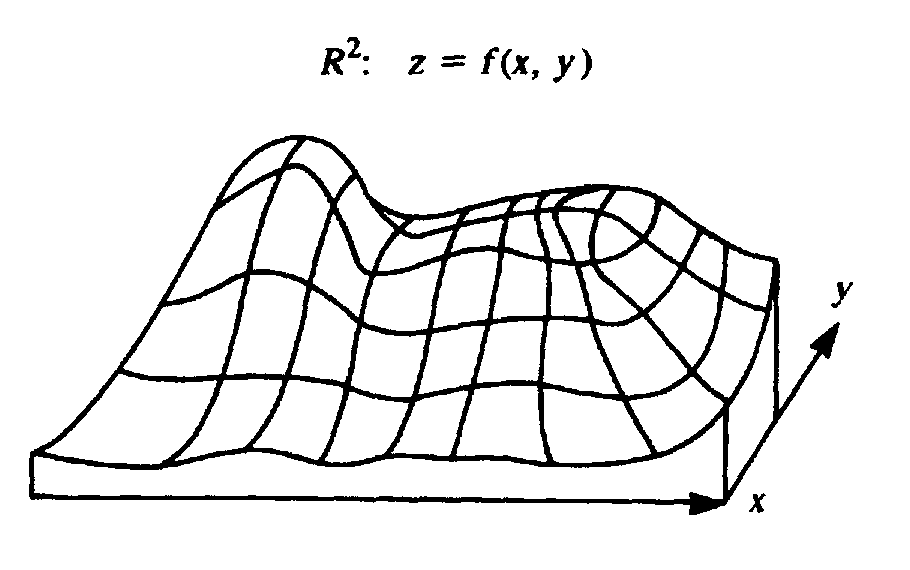
\includegraphics[scale=0.3]{figs/leah/fig09.01a.png}
\caption{\small uma superfície (apenas duas variáveis)}
\label{fig:09.01a}
\end{subfigure}
\begin{subfigure}[t]{0.33\linewidth}\centering
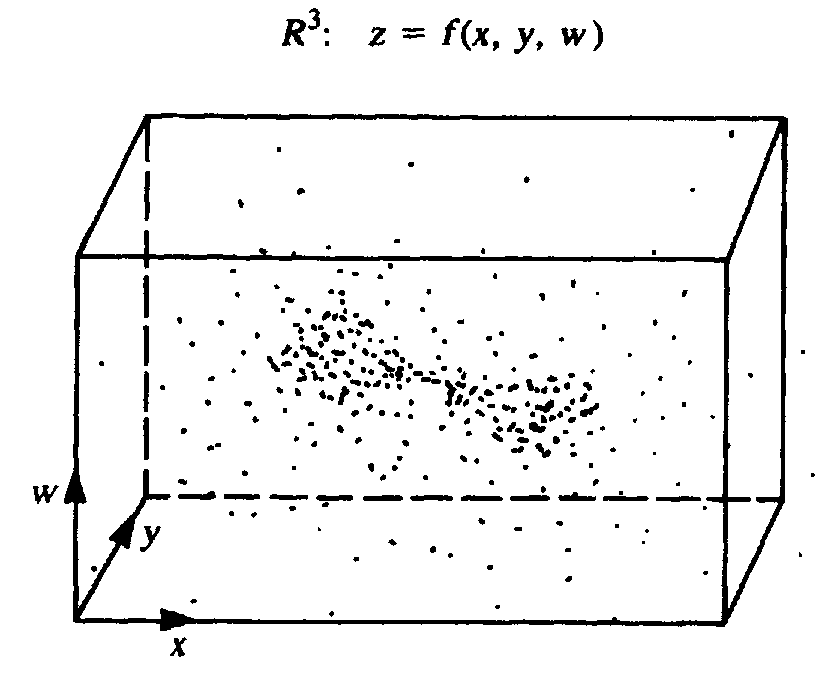
\includegraphics[scale=0.3]{figs/leah/fig09.01b.png}
\caption{\small uma distribuição de densidade no R3}
\label{fig:09.01b}
\end{subfigure}
\begin{subfigure}[t]{0.32\linewidth}\centering
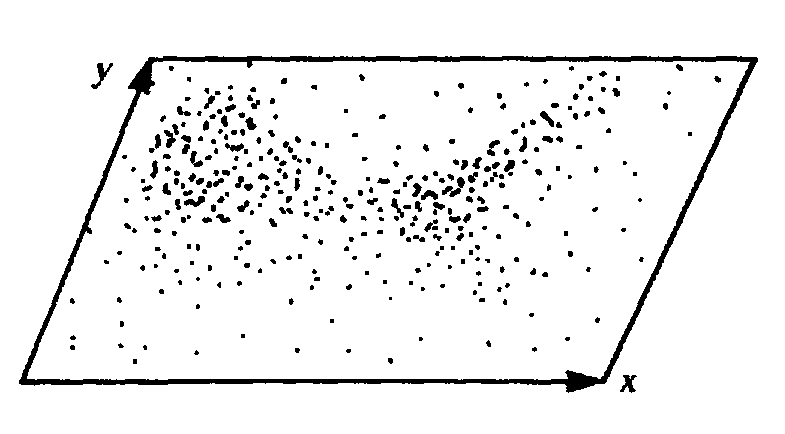
\includegraphics[scale=0.3]{figs/leah/fig09.01c.png}
\caption{\small uma distribuição de densidade no R2}
\label{fig:09.01c}
\end{subfigure}
\vfil
\begin{subfigure}[t]{0.5\linewidth}\centering
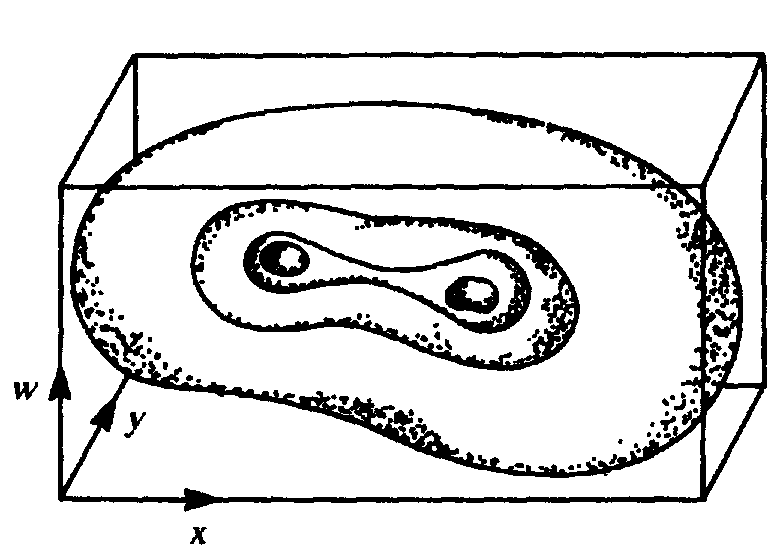
\includegraphics[scale=0.3]{figs/leah/fig09.01d.png}
\caption{\small superfície de nível}
\label{fig:09.01d}
\end{subfigure}
\begin{subfigure}[t]{0.5\linewidth}\centering
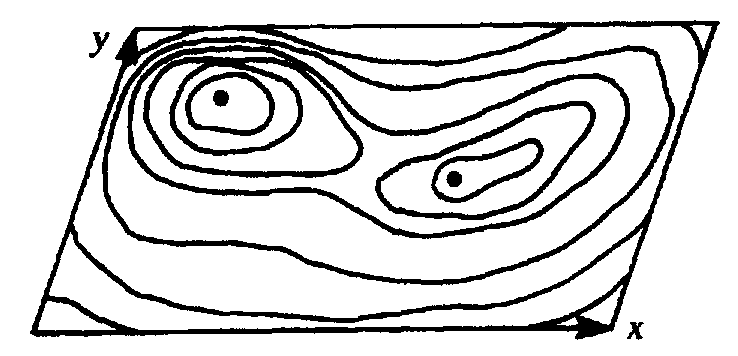
\includegraphics[scale=0.3]{figs/leah/fig09.01e.png}
\caption{\small curvas de nível}
\label{fig:09.01e}
\end{subfigure}
\end{figure}



\begin{comment}
In R3 the function of three variables given by (2) can similarly be represented by sets of points for which f(x, y, w) = constant. (4)
\end{comment}
%\begin{comment}
Em R3, a função de três variáveis dadas por (2) pode ser representada de forma semelhante por conjuntos de pontos para os quais
\begin{equation}\label{eq:09.04}
f(x, y, w) = \mathrm{constante}.
\end{equation}
%\end{comment}

\begin{comment}
Such loci area generalized version of level curves, but for obvious reasons these are called level surfaces [see Figure 9.1(d)]. To clarify with an example, consider a temperature field in three dimensions. The equitherms are then surfaces at which some given constant temperature is maintained. If heat sources are located at two points, the resulting equithermal surfacesmight look something like those shown in Figure 9.1(d).
\end{comment}
%\begin{comment}
Esses loci são uma versão generalizada das curvas de nível, mas por razões óbvias são chamadas de superfícies de nível [ver Figura 9.1 (d)]. Para esclarecer com um exemplo, considere um campo de temperatura em três dimensões. Os equitérmos são, então, superfícies nas quais uma dada temperatura constante é mantida. Se as fontes de calor estiverem localizadas em dois pontos, as superfícies equitérmicas resultantes podem se parecer com as mostradas na Figura 9.1 (d).
%\end{comment}


\begin{comment}
In the context of this chapter, level curves or surfaces might represent the loci on which (1) population density is constant or (2) chemical concentration is constant.

We shall be concerned primarily with statements about how spatial distributionschange with time; frequently it will be clear that the movement of one substance or population is closely linked to the distribution of another.

Consider the following simple example.An organism crawling on a flat surface may adapt its motion to the search for food particles. Imagine then that the dots in Figure 9.1(c) represent nutrient particle concentration. The observed path should ideally lead to the site of greatest concentration. To sense an increase in the ambient concentration level, an organism must continually cross level curves of the particle distribution. Per unit distance traveled, this crossing can be done most efficientlyby maintaining a path orthogonal to the level curves;in other words, a tangent vector to the path should be perpendicular to a tangent to a level curve through a given point. This assertion can be verified using rather elementary calculus of several variables. It can alsobe shown that the destination will be a critical point of the function (in this case a local maximum) but not necessarily the global maximum.
\end{comment}
%\begin{comment}
No contexto deste capítulo, curvas de nível ou superfícies podem representar os loci nos quais (1) a densidade populacional é constante ou (2) a concentração química é constante.

Estaremos preocupados principalmente com afirmações sobre como as distribuições espaciais mudam com o tempo; frequentemente ficará claro que o movimento de uma substância ou população está intimamente ligado à distribuição de outra.

Considere o seguinte exemplo simples. Um organismo rastejando sobre uma superfície plana pode adaptar seu movimento à procura de partículas de alimento. Imagine então que os pontos na Figura 9.1 (c) representam a concentração de partículas de nutrientes. O caminho observado deve, idealmente, levar ao local de maior concentração. Para sentir um aumento no nível de concentração ambiente, um organismo deve cruzar continuamente as curvas de nível da distribuição de partículas. Por unidade de distância percorrida, esse cruzamento pode ser feito de forma mais eficiente, mantendo um caminho ortogonal às curvas de nível; em outras palavras, um vetor tangente ao caminho deve ser perpendicular a uma tangente a uma curva de nível através de um determinado ponto. Esta afirmação pode ser verificada usando cálculos bastante elementares de várias variáveis. Também pode ser mostrado que o destino será um ponto crítico da função (neste caso, um máximo local), mas não necessariamente o máximo global.
%\end{comment}


\begin{comment}
In calculus a common place analogy is often drawn in explaining these ideas. Hikers often use topographical maps which are two-dimensional representations of the height of the terrain. The curves on such maps are level curves for the function f(x, y) = height above sea level at latitude x and longitude y. Mountain peaks, valleys, and mountain passes are critical points off(x, y) that correspond to local maxima, minima, and saddle points respectively. Using local information only (for example, walking uphill with no information other than the local slope), one can attain a local maximum, but this may or may not be the highest possible peak.
\end{comment}
%\begin{comment}
No cálculo, uma analogia comum é frequentemente desenhada para explicar essas ideias. Os caminhantes costumam usar mapas topográficos que são representações bidimensionais da altura do terreno. As curvas em tais mapas são curvas de nível para a função $f(x, y) =$ altura acima do nível do mar na latitude $x$ e longitude $y$. Os picos das montanhas, vales e passagens nas montanhas são pontos críticos fora $(x, y)$ que correspondem aos pontos máximos, mínimos e de sela locais, respectivamente. Usando apenas informações locais (por exemplo, subindo uma colina sem nenhuma informação além da inclinação local), pode-se atingir um máximo local, mas este pode ou não ser o pico mais alto possível.
%\end{comment}


\begin{comment}
These two-dimensional examples can be extended to higher dimensions. A motile organism that swims in a droplet of water might also use local cuesin orienting itself and moving towards sites mat have higher nutrient levels. This type of motion, called chemotaxis, will be discussed at greater length in Section 10.2. In R3 the path of a highly efficient chemotactic organism would be orthogonal to the level surfaces of the nutrient distribution c(x, y, z).
\end{comment}
%\begin{comment}
Esses exemplos bidimensionais podem ser estendidos para dimensões superiores. Um organismo móvel que nada em uma gota d'água também pode usar dicas locais para se orientar e se mover em direção a locais com níveis mais elevados de nutrientes. Esse tipo de movimento, denominado quimiotaxia, será discutido com mais detalhes na Seção 10.2. Em R3, o caminho de um organismo quimiotático altamente eficiente seria ortogonal às superfícies de nível da distribuição de nutrientes $c(x, y, z)$.
%\end{comment}


\begin{comment}
The descriptiv estatements in this section can be made more rigorousby introducing partial derivatives and gradients which are reviewed in the boxed material.

Several examples follow the general discussion and definitions.
\end{comment}
%\begin{comment}
Os estatutos descritivos nesta seção podem ser feitos mais rigorosos pela introdução de derivados parciais e gradientes que são revisados no material em caixa.

Vários exemplos seguem a discussão geral e as definições.
%\end{comment}


\begin{comment}
\subsection{Partial derivatives (A Review)}
\end{comment}
%\begin{comment}
\subsection{Derivadas Parciais (Revisão)}
%\end{comment}



\begin{comment}
For a function of two variables f(x, y) we define
\begin{equation}
\dfrac{\partial f}{\partial x} = \lim_{\Delta x \to 0} \dfrac{f(x+\Delta x, y) - f(x,y)}{\Delta x}
\end{equation}
A similar definition holds for df/dy. Shorthand notation for partial derivatives is fx and fy.
\end{comment}
%\begin{comment}
Para uma função de duas variáveis $f(x,y)$, definimos:
\begin{equation}\label{eq:09.05}
\dfrac{\partial f}{\partial x} = \lim_{\Delta x \to 0} \dfrac{f(x+\Delta x, y) - f(x,y)}{\Delta x}
\end{equation}
Uma definição semelhante é válida para $\dfrac{\partial f}{\partial y}$. A notação abreviada para derivadas parciais é $f_x$ e $f_y$.
%\end{comment}


\begin{comment}
To understand the geometrical meaning of these derivatives, imagine standing at a point (x0, y0) on a plane. Suppose f(x0, y0) is the height of a surfaceabovethis location. The expression following ``lim'' in equation (5) (and similarly for df/dy) represents the changes in the height of the surface per unit distance as we take a step in the x (or the y) direction. A partial derivative is the limit of this quantity as the length of the step shrinks to an infinitesimal size. It is therefore analogous to an ordinary derivative and also represents a slope.
\end{comment}
%\begin{comment}
Para entender o significado geométrico dessas derivadas, imagine estar em um ponto (x0, y0) em um plano. Suponha que f (x0, y0) seja a altura de uma superfície acima desta localização. A expressão após `` lim '' na equação (5) (e da mesma forma para df / dy) representa as mudanças na altura da superfície por unidade de distância conforme damos um passo na direção x (ou y). Uma derivada parcial é o limite dessa quantidade, pois o comprimento da etapa diminui a um tamanho infinitesimal. É, portanto, análogo a uma derivada comum e também representa uma inclinação.
%\end{comment}


\begin{comment}
To clarify, suppose we slice away part of the surface z = f(x, y) along a direction parallel to the x (or y) axis. (See Figure 9.2.) In such cutaway drawings the partial derivative is the slope of a tangent to the curve forming the surface edge. The idea of a partial derivative is a special case of the somewhat more general concept of directional derivative. We shall not deal in more depth with this but rather refer the reader to any standard calculus text for a definition and explanation.
\end{comment}
%\begin{comment}
Para esclarecer, suponha que cortamos parte da superfície $z = f(x, y)$ ao longo de uma direção paralela ao eixo $x$ (ou $y$). (Veja a Figura 9.2.) Em tais desenhos de cortes, a derivada parcial é a inclinação de uma tangente à curva que forma a borda da superfície. A ideia de uma derivada parcial é um caso especial do conceito um tanto mais geral de derivada direcional. Não trataremos disso com mais profundidade, mas antes encaminharemos o leitor a qualquer texto de cálculo padrão para uma definição e explicação.
%\end{comment}

\begin{figure}[!ht]
%\caption{\small An interpretation of partial derivatives and gradient vectors. The surface z = f(x, y) intersects planes for which y = constant or x = constant along curves ell 1 and ell 2. The slope of a tangent to ell_1 is df/dx, and the slope of a tangent to ell_2 is df/dy. Gradient vectors, \nabla f [for f = f(x, y)] live in the xy plane and have (df/dx, df/dy) as components. These vectors are always orthogonal to level curves of z = f(x, y), shown here by dashed lines (see inset).}
\caption{\small Uma interpretação de derivadas parciais e vetores gradientes. A superfície $z = f(x, y)$ intersecta planos para os quais $y =$ constante ou $x =$ constante ao longo das curvas $\ell_1$ e $\ell_2$. A inclinação de uma tangente para $\ell_1$ é $\dfrac{\partial f}{\partial x}$, e a inclinação de uma tangente para $\ell_2$ é $\dfrac{\partial f}{\partial y}$. Os vetores gradientes, $\nabla \mathbf{f}$ [para $\mathbf{f} = f(x, y)$] vivem no plano $xy$ e têm ($\partial \mathbf{f} / \partial x, \partial \mathbf{f} / \partial y$) como componentes. Esses vetores são sempre ortogonais às curvas de nível de $z = f(x, y)$, mostradas aqui por linhas tracejadas (ver inserção).
}
\centering
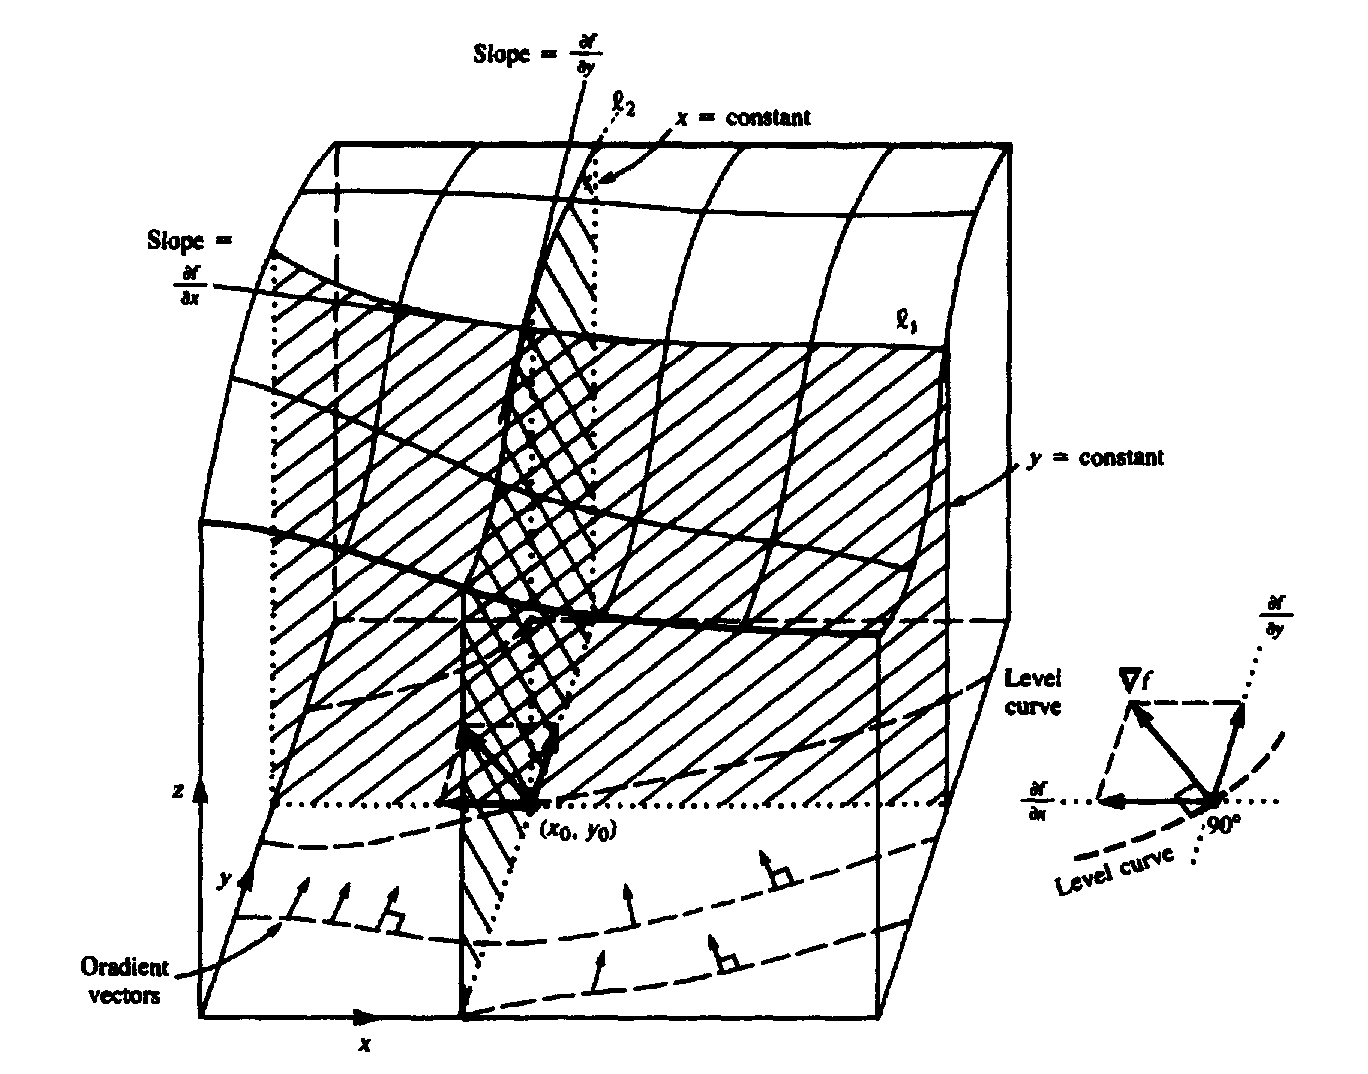
\includegraphics[scale=0.5]{figs/leah/fig09.02.png}
\label{fig:09.02}
\end{figure}


\begin{comment}
The following properties of partial derivatives follow from their basic definition: ir-cTx'
m
dx dx dx,

for functions /and g and constant c. Similar equations ensue for partial differentiation with respect to y.

For functions that are continuously differentiable sufficiently many times, it is also true that mixed partial differentiation in any order produces the same result. For example
fyx = partial \partial x(\partial f \partial y )

Note: Equation (6c) also defines the equivalent notation used for multiple partial differentiation.
\end{comment}
%\begin{comment}
As seguintes propriedades de derivadas parciais seguem de sua definição básica:
\begin{eqnarray}\label{eq:09.06ab}
\dfrac{\partial (cf+g)}{\partial x} = c\dfrac{f}{\partial x} + \dfrac{g}{\partial x},
\end{eqnarray}
para funções $f$ e $g$ e constante $c$. Equações semelhantes resultam da diferenciação parcial em relação a $y$.

Para funções que são continuamente diferenciáveis o suficiente muitas vezes, também é verdade que a diferenciação parcial mista em qualquer ordem produz o mesmo resultado. Por exemplo
\begin{eqnarray}\label{eq:09.06c}
f_{yx}
= \dfrac{\partial}{\partial x} \left(\dfrac{\partial f}{\partial y}\right)
= \dfrac{\partial^2 f}{\partial x \partial y} 
= \dfrac{\partial^2 f}{\partial y \partial x}
= \dfrac{\partial}{\partial y} \left(\dfrac{\partial f}{\partial x}\right)
= f_{xy}
\end{eqnarray}

\textbf{Nota}: A Equação (6c) também define a notação equivalente usada para diferenciação parcial múltipla.
%\end{comment}

\begin{comment}

\end{comment}
%\begin{comment}

%\end{comment}

\begin{comment}

\end{comment}
%\begin{comment}

%\end{comment}

\begin{comment}

\end{comment}
%\begin{comment}

%\end{comment}

\begin{comment}

\end{comment}
%\begin{comment}

%\end{comment}

\begin{comment}

\end{comment}
%\begin{comment}

%\end{comment}








% AQUI ESTOU PULANDO
\begin{comment}







gradients

For a function/of several variables the gradient, symbolized Vf, is a vector consisting of the partial derivatives off. For example,if/ =f(x, y), then
Uf = f(x,y,z), then
(7)
(8)
and so on for functions of n variables. The symbol V is called the del operator, and is discussed in greater detail in Section 9.3. The gradient vector has the following properties:

1. The magnitude of Vf, \\Vf |, represents the steepness of the local variations in the
function/. For example,
lYM
= (/,2+//),/2. (9)



2.

(a) The direction of V/, is a unit vector in the direction of steepest(increasing) slope, in the sense
that a step in this direction leads to the greatest increasein/per unit distance,
(b) The gradient vector at a point (xq, Vq) is perpendicular to a level curve
fix, y)
= c that goes through fa, yo) as long as (x0, yo) is not a local maximum, minimum, or saddle point.
For every point in R2 (analogously, R3 or R\") at which the function /is defined,
is continuous, and has partial derivatives, there will be a gradient vector. The vector
will have all zero components at the critical points of/.
It is common to visualize a whole collection of these vectors, one at each point in
space, as a vectorfield. A vector field that arises thus is called a gradient field and has
certain special properties. (Note that a gradient field is a vector field, but the converse
is not necessarilytrue.)

    Gradient fields can always be paired (up to an arbitrary constant) with differentiable multivariate functions and vice versa (see examples in the following boxes). We see that the variations in a spatial distribution lead to orientation cues that are represented by the geometry of the gradient field.

    The proof of the statements in this box are basedon the chain rule of functions of several variables and on the properties of curves and vector dot products. These can be found in any text dealing with the calculus of several variables.


Example1
Consider the function
fix, y) = x2 - 2x + y2 + Ay + 5.
Level curves of this function have the equation
c = x2-
-(*-
2x+ y2 + Ay + 5
D2 + (y + 2f.
These are circles of radius c'/2 centeredat the point (1, -2).
fix, y) are the following:
dx
d2f = o,
dx dy
dx2
lt
2, | = 2y + 4,
dy
*f = o,
dy dx
3y2
2'

The gradient vector at a point (x, y) is
*-(&#-*->.*
+ *
This vector is perpendicular to a level curve going through the point (x, y). A
critical point of/occurs at (1, -2), where Vf
= (0, 0). At this point,/(l, -2) = 0. At
any other point/is greater. For example,/(l, 1)= 1-2+1+4 + 5 = 9.
Therefore(1, -2) is a local minimum. (A more rigorous second-derivative test to distinguish
between local minima, maxima, and saddle points is given in most calculus books).


Example 2
Considerthe vector field
F = (M(x,
= (2x +
y), N{x, y))
2y + y cos xy,2x -\\- x cos xy).
We would like to determine whether F is a gradient field, that is
function fix, y) such mat
F
If so, then
F
whereM(x,y)
= df/dx and N =
By a previous observation
dy
fxy
Checking this, we note that
= V/.
-<\"\342\200\242\302\273-(!\342\200\242#\342\200\242
df/dy.
we must have
hx
dx'
dM \342\200\236 dN
\342\200=\224 2 + cos xy
- xy sin xy
=
 --- ,
dy
J J dx
(10)
i, whether there is a
Ola)
(Ub)
(12)
so that no contradiction results by assuming that (11a) holds. The condition given by
(12) in fact guarantees that F is a gradient field (a fact whose proof will be omitted
here).
To find /we need a function whose partial derivatives satisfy the following:
3/
dx
a/
dy
= 2x + 2y + y cos xy,
= 2x + x cos xy.
(13a)
(13b)


Integrating each expression with respect to a single variable while holding the other
variable constant leads to these results:
f(x, y)
= (2x + 2y + y cos xy)dx (14)
\342\200\242/(y-conw)
= x2 + 2xy + sin xy + H,
and
fix, y)
= (2x + x cos xy)dy (15)
J (r --- const)
= 2xy + sinxy + G.
In ordinary one-variable calculus, a single integration introduces a single arbitrary
constant. However, in the partial integration of (14) and (15) one must account for the
distinct possibility that the integration \"constants\" H and G may depend on the values
given to the fixed variables (to y = const and to x = const). For this reason it is
necessaryto presuppose that
H = h(y) and G = g(x) (16)
are functions. Indeed, the only possibility for matching the two different expressions,
(14)and (IS), both of which equal the same function/(x, y), would be to take
G(x)
= x1 + c, H(y) = c,
for constant c.
The conclusion then is that
f(x, y) = x2 + 2xy + sin xy + c. (17)
To checkthis result, observe that
Vf = (2x + 2y
- y cos xy, 2x - x cos xy)
= F,
which confirms the calculation. Note that adding any constant to f(x, y) results in the
same gradient. Thus/(x, y) is defined only up to some arbitrary additive constant.



Example 3
The concentration of nutrient particles suspended in a pond is given by the expression
c(x, y, z)
= Co exp -a(x2 + y2 + z2). (18)
An organism located at (x, y, z) = (1, -1, 1)moves in the direction of increasing
concentration. In which direction should it move? Where is the maximum concentration?
Answer
To find the direction of greatest increaseperunit distance, compute the gradient vector.
Sincec is a function of three variables, Vc is a vector in R3:
(dc dc dc\\
Vc =
\\Tx'Ty>i;)
<19a>
= (-2axC0e-'\"2,-2ayC0e-'\"1-,2azC0e-'\"1), (19b)

where
r2 = x2 + y2 + z2 (19c)
at(l, -1, 1)
r2 = 3 and Vc = (-y, y, -y),
where
y = 2aC0e-3a.
Furthermore, Vc = 0 only when (x, y, z) = (0, 0, 0), sothat the origin is a
critical point. It is readily observedthat this is a local maximum, since c(x,y, z) is a
function that decreases exponentially with distance from the origin. Thus, the maximal
concentration of nutrient particles is c(0, 0,0) = C0. We further observe that equiconcentration
loci are surfaces that satisfy
Co exp -a(x2 + y2 + z2) = constant. (20a)
After algebraic simplification this becomes
x2 + y2 + z2 = K (K = constant), (20b)
which represents spheres with centers at (0, 0, 0) and radii VAT.
Thus the organism will move in the direction of the gradient, and its path will
eventually end at (0, 0, 0).


In the next section our purpose is to understand the basic processthrough which a
partial differential description of motion through space is obtained. We shall be
concerned mainly with the dynamic processes that lead to changes in a spatial
distributioonver time. Some of the many examplescited pertain to the motion and
continuoruesdistribution of animals, cells, and molecules through space. For this reason we
shall dealwith functions that depend on both space and time

\end{comment}


\section{UMA RÁPIDA DERIVAÇÃO DA EQUAÇÃO DE CONSERVAÇÃO}


A equação de conservação em suas várias formas é a declaração mais fundamental por meio da qual as mudanças nas distribuições espaciais são descritas. A maioria dos EDP que encontraremos baseia-se basicamente nessas declarações de equilíbrio. Para obter uma familiaridade fácil com os conceitos básicos, consideraremos um caso bastante especial e daremos primeiro uma derivação informal, para posteriormente ser mais rigorosa e geral.

Nossas suposições iniciais são que:

1. O movimento ocorre em uma única dimensão espacial (como, por exemplo, no tubo fino da Figura 9.3a).

2. A seção transversal do navio ou contêiner é constante ao longo de todo o seu comprimento.

Devemos deixar $x$ representar a distância ao longo do tubo de algum local arbitrário. Fixando a atenção no intervalo entre $x$ e $x + \Delta x$, vamos descrever as mudanças na concentração, considerando dois efeitos possíveis:

(1) fluxo de partículas para dentro e fora do intervalo $(x, x + \Delta x)$ e

(2) processos que introduzem novas partículas ou degradam partículas localmente (como por meio de uma reação química).


\begin{figure}[!ht]
\caption{\small Equações de equilíbrio são derivadas para o fluxo de partículas [concentração $c(x, t)$] ao longo de um tubo, (a) Se o tubo tem área transversal $A$ uniforme, a equação (24) resulta de um equilíbrio de fluxos para dentro e para fora de uma pequena seção (b) de comprimento $\Delta x$. (c) Se o tubo tem uma área $A(x, t)$ que varia espacial ou temporalmente, obtém-se a equação (29) formulando o balanço para a pequena região mostrada em (d).}
\centering
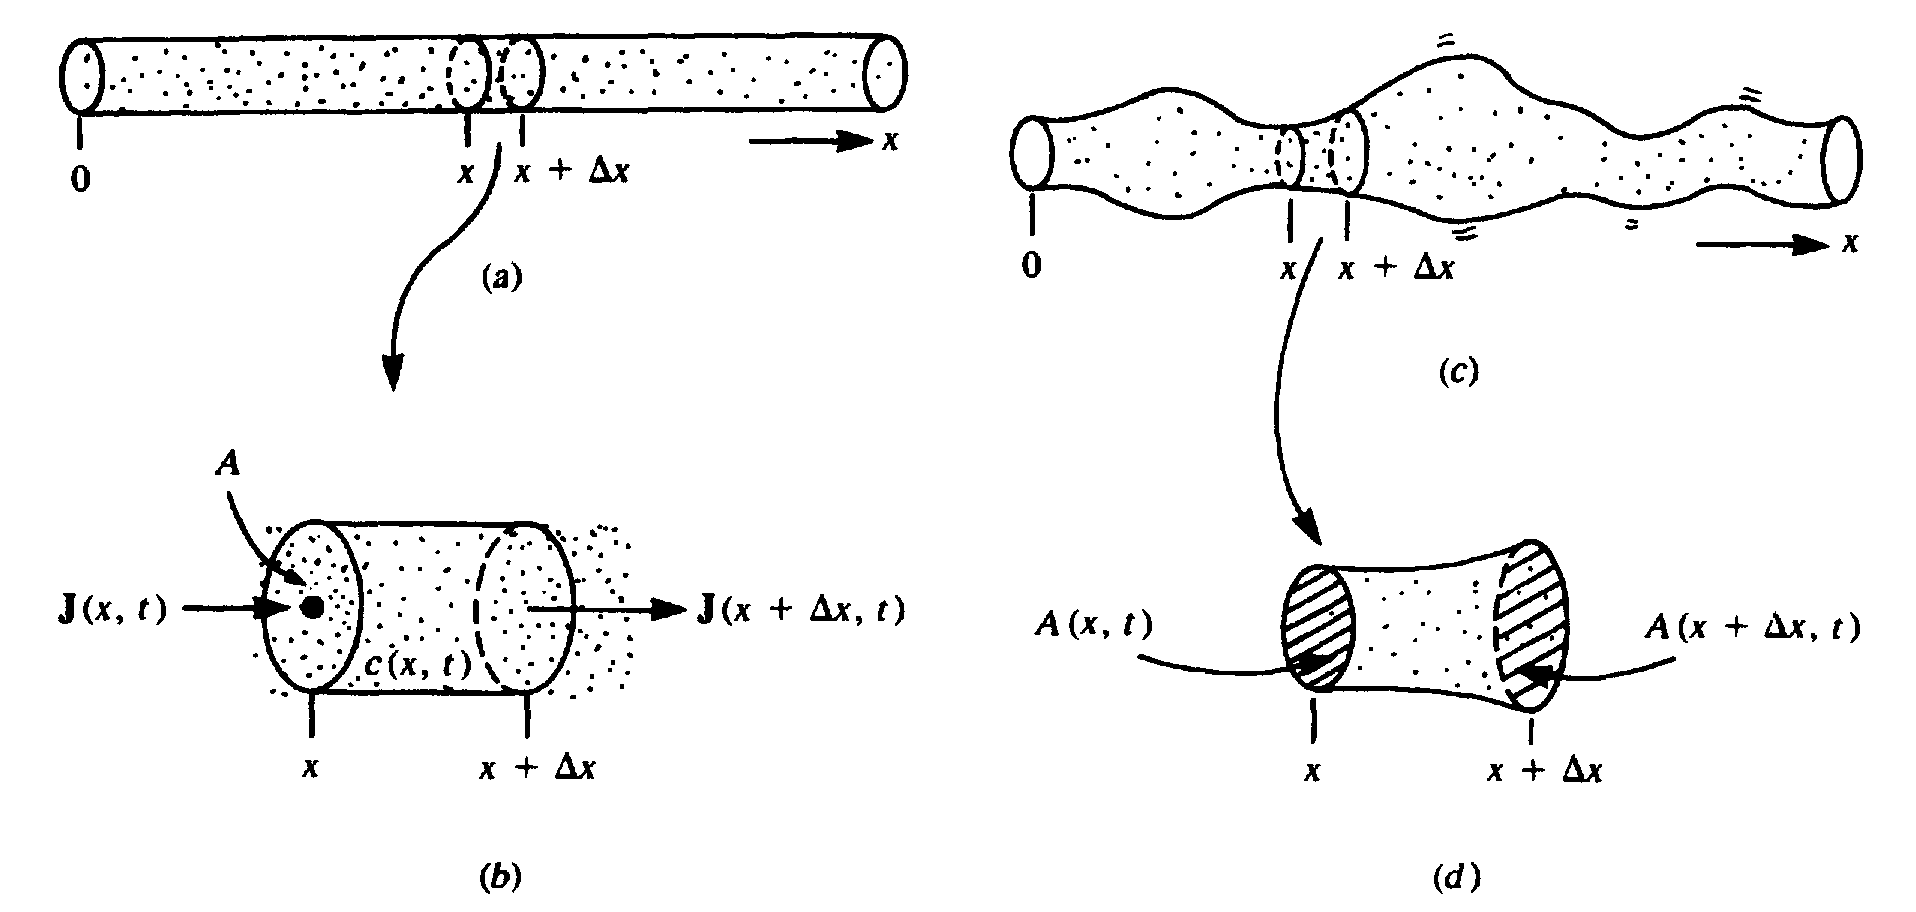
\includegraphics[scale=0.5]{figs/leah/fig09.03.png}
\label{fig:09.03}
\end{figure}

A equação de equilíbrio pode ser escrita em termos de massa ou número de partículas. Nós escolhemos arbitrariamente a última descrição e, portanto, nossa declaração será
$$
\left[
\begin{tabular}{m{0.15\textwidth}}\tiny
taxa de mudança da população de partículas em $(x, x + \Delta x)$ por unidade de tempo
\end{tabular}
\right]
=
\left[
\begin{tabular}{m{0.15\textwidth}}\tiny
taxa de entrada em $(x, x + \Delta x)$ por unidade de tempo
\end{tabular}
\right]
-
\left[
\begin{tabular}{m{0.15\textwidth}}\tiny
taxa de partida de $(x, x + \Delta x)$ por unidade de tempo
\end{tabular}
\right]
\pm
\left[
\begin{tabular}{m{0.15\textwidth}}\tiny
taxa de degradação local ou criação por unidade de tempo
\end{tabular}
\right]
$$


Para ir além, defina as seguintes quantidades:

$c(x, t) =$ concentração de partículas (número por unidade de volume) em $(x, t)$,

$J(x, t) =$ fluxo de partículas em $(x, t)$ = número de partículas cruzando uma área unitária em $x$ na direção positiva por unidade de tempo,

$\sigma (x, t) =$ densidade de sumidouro / fonte = número de partículas criadas ou eliminadas por unidade de volume em $(x, t)$.


Notamos que o único fluxo que altera a população total é aquele que entra ou sai pelas seções transversais em $x$ e $x + \Delta x$, a saber, $J(x, t)$ e $J(x + \Delta x, r)$.

Para agora traduzir (21) em uma equação dimensionalmente correta, é necessário levar em consideração as seguintes quantidades:

$A =$ área da seção transversal do tubo,

$\Delta V =$ volume do elemento de comprimento $\Delta x = A \Delta x$.

Cada termo na equação deve ter as mesmas unidades que os termos no LHS de (21): número por unidade de volume por unidade de tempo.

Isso leva à seguinte equação:
$$\dfrac{\partial}{\partial t} [c(x, t) A \Delta x]
= J(x, t) A - J(x + \Delta x, t) A \pm \sigma(x, t) A \Delta x.
%(22)
$$

Observe que, como $c$ depende de duas variáveis, sua derivada em relação ao tempo é uma derivada parcial. Escolher escrever a equação (22) em termos de $x$, a coordenada do limite esquerdo do intervalo, é totalmente arbitrário, pois estamos prestes a tomar o limite $\Delta x \to 0$.

Observamos que um fluxo na direção $x$ positiva tende a contribuir para a população líquida positivamente em $x$, mas negativamente em $x + \Delta x$; daí os sinais dos termos em (22). Veja a Figura 9.3 (b).

Agora, dividindo por $A \Delta x$, que por suposição é constante, obtemos:
$$
\dfrac{\partial}{\partial t} c(x, t) = \dfrac{J(x, t) - J(x + \Delta x, t)}{\Delta x} \pm \sigma(x, t).
%(23)
$$





Tomando o limite desta equação como $\Delta x \to 0$, como a largura da fatia fica cada vez menor, chegamos a uma afirmação local, a equação de equilíbrio unidimensional,

$$
\dfrac{\partial}{\partial t} c(x, t) = \underbrace{-\dfrac{\partial J(x, t)}{\partial x}}_{\textrm{movimento líquido}} \pm \underbrace{\sigma(x, t)}_{\textrm{fonte / dissipador}}.
%(23)
$$

O sinal negativo em $\partial J / \partial x$ deriva do fato de que a diferença finita em (23) tem um signo oposto àquele na definição de uma derivada.

Esta é a forma básica da lei de equilíbrio que em breve aplicaremos a vários problemas específicos. Antes disso, faremos uma série de extensões e declarações gerais. É possível pular este material e ir para a Seção 9.4 sem perda de continuidade.




\section{OUTRAS VERSÕES DA EQUAÇÃO DE CONSERVAÇÃO}

\subsection{Fluxo tubular}

Devemos abandonar a suposição (2) e considerar a possibilidade de que a área da seção transversal do tubo pode variar no espaço e no tempo. Para ser um pouco mais formal, tomamos as seguintes definições: Pela concentração $c(x, t)$ queremos dizer uma quantidade tal que

$\displaystyle \int_{x_1}^{x_2} c(x, t) A(x, t) dx =$ número total de partículas localizadas dentro do tubo no intervalo $(x_1, x_2)$ no tempo $t$.
%(25a)


Da mesma forma, a densidade da fonte $\sigma(x, t)$ é definida por

$\displaystyle \int_{x_1}^{x_2} \sigma(x, t) A(x, t) dx =$ taxa de criação ou degradação de partículas dentro do intervalo $(x_1, x_2)$ no tempo $t$.
(25b)
 
A equação de equilíbrio pode então ser escrita na forma integral (às vezes chamada de forma fraca), como segue:

$$
\dfrac{\partial}{\partial t} \dint_{x_0}^{x_0+\Delta x} c(x, t) A(x, t) dx 
=
J(x_0, t) A(x_0, t) - J(x_0 + \Delta x, t) A(x_0 + \Delta x, t) \pm \dint_{x_0}^{x_0+\Delta x} \sigma(x, t) A(x, t) dx.
%(26)
$$

(Isso é semelhante a uma derivação em Segel (1980, 1984) para área constante.)

Um teorema do valor médio integral permite concluir que em alguns locais
$(x_1, X_2)$ (onde $x_0 \le x_i \le x_0 + \Delta x$, para $i = 1, 2$) o seguinte é verdadeiro:

$$\dfrac{\partial}{\partial t} [c(x_1, t) A(x_1, t)] \Delta x
= J(x_0, t) A(x_0, t) - J(x_0 + \Delta x, t) A(x_0 + \Delta x, t) \pm \sigma(x_2, t) A(x_2, t) \Delta x.
%(27)
$$


Agora dividindo por $\Delta x$ e deixando $\Delta x \to 0$, obtemos $x_1 \to x_0$ e $x_2 \to x_0$, que na equação limite (27 ) torna-se


$$\dfrac{\partial}{\partial t} [c(x_0, t) A(x_0, t)]
= -\dfrac{\partial}{\partial x} [J(x_0, t) A(x_0, t)] \pm [\sigma(x_0, t) A(x_0, t)].
%(28)
$$

\subsection{Casos especiais}



1. Se $A(x_0, t) = A$ for constante, dividir por $A$ reduz a equação (28) à equação (24).

2. Se $A(x, t) = A(x) \neq 0$ (ou seja, se a área não muda com o tempo), a equação pode ser escrita na forma
$$
\dfrac{\partial}{\partial t} c(x, t)
= - \dfrac{1}{A(x)} \dfrac{\partial}{\partial x} [J(x, t) A(x)] \pm \sigma(x, t).
%(29)
$$

Quando a derivada parcial é expandida, obtém-se:
$$
\dfrac{\partial}{\partial t} c(x, t)
= - \dfrac{\partial}{\partial x} J(x, t) - \dfrac{J(x, t)}{A(x)} \dfrac{\partial}{\partial x} A(x) \pm \sigma(x, t).
%(30)
$$


A equação é, portanto, semelhante a (24), mas contém um termo extra que explica um efeito semelhante à diluição; ou seja, uma mudança na concentração que decorre de mudanças locais no volume do fluido "sentido" pelas partículas à medida que se movem ao longo do comprimento do tubo.

3. Se $A(x, t) = A (t) \neq 0$ (se a área do tubo for uniforme ao longo de seu comprimento, mas possivelmente variando no tempo), então a equação (28) leva ao seguinte:
$$
A(t) \dfrac{\partial}{\partial t} c(x,t) + c(x,t) \dfrac{\partial}{\partial t} A(t) = - A(t) \dfrac{\partial}{\partial x} J(x,t) \pm \sigma(x,t) A(t).
%(31)
$$

Depois de alguns rearranjos, isso se torna:
$$
\dfrac{\partial}{\partial t} c(x,t) = - \dfrac{c(x,t)}{A(t)} \dfrac{\partial}{\partial t} A(t) - \dfrac{\partial}{\partial x} J(x,t) \pm \sigma(x, t).
%(32)
$$

Mais uma vez, a equação se assemelha a (24), com um termo adicional que, grosso modo, também descreve um efeito de diluição conforme o tubo se expande ou se contrai.

4. Em uma situação onde a área da seção transversal varia tanto espacialmente quanto temporalmente $[A = A(x, t)]$, segue-se que a equação (28) pode ser escrita

dc (x, t) _ dj (x, t), 1 L, .i dA (x, t)








\begin{comment}








Flows in Two and Three Dimensions

To write a balance equation analogous to (24) in higher dimensions we consider a
small rectangular element of volume AV =
AxAyAz situated in R3 and account for
motion of particlesinto and out of the region. First it proves necessary to extend
somewhatour definition of flux, for now both direction and magnitude of flow have
to be considered.
Let us focus attention on a point (xo, yo, z0) in R3. We shall define flux by
counting the number of particlesperunit time that traverse an imaginary unit area A
suspended at (xo, yo, z0) with some particular orientation. As the orientation of the
\"test area\" is varied, the rate of crossingschangesIn.deed, the highest rate of
crossingis achieved when the predominant flow direction is orthogonal to the area that it
must cross. This leads us to defineflux as a vector in the direction n whose
magnitudeis given by:
net number of particles crossing
I J(*, y> z, t) I = a unit area at (x, y, z) per (34)
unit time at time t
where n is the unit normal vector to that element of area that admits the greatest net
crossings. [See Figure 9.4(a).]
We shall symbolize the components of J (in R3) as follows:
J(x, y,z) = (Jx,Jy, Jt). (35)
Each of the components Jx, Jy, and Jz may in general depend on both space and
time.
In three dimensionsthe magnitude of flux is given by the quantity
I j |
= {Ji + p, + W2 = (j \342\200\242
j),/2 (36)
(where
-
represents a vector dot product).Given some test area A, this definition of
flux allows one to calculate the number of particle crossings N that take place in a
given time f. If m is a unit vector perpendicular to the test area, one obtains
N= (J-m)A Ar. (37)



Figure 9.4 \caption{(a)In R3 flux J is a vector. Its
magnitude represents the net number of particles
crossing an imaginary unit area per unit time. Its
direction is given by the normal vector n to the
given area A. (b) Theequation of conservation
(39) is derived by considering net flow into a small
rectangular volume of dimensions Ax X Ay X Az.}



To illustrate this idea, considera wall of unit area at the point (-1,0, 3) orthogonal
to the direction m = (1, 0, 0),and a flux J = (z -
y, x  --- 
z, y
 --- 
x). At the point in
question,
J = (3, -4, 1),



so that the number of crossings is
N = (J m) lAr = [(3, -4, 1) \342\200\242
(1, 0, 0)] At = 3At.
Thus three particles traverse the wall per unit time.
Given a small rectangular volume as shown in Figure 9.4(b), the statement of
balancemust accommodate, as before, local creation and entry or departure through
each of the six planar surfaces. Since these planes are parallel to the coordinate
planes, we can readily determine their normal vectors and calculate the net number
of particles crossing (inwards) through each wall. (See Table 9.1.)
The net rate of change of concentration inside the volume that accrues from
combining all thesefactors is the following:
dc _ Jx(xq, y0> zo)
- Jx(xp + Ax, yo, z0)
dt Ax
. /y(*o> yo. zo) -
4\302\273(*o>yo + Ay. z0)
Ay
+
Uxo,yo,zo)-Uxo,y0,z0 + Az)
\302\2^61 ^ ^ ^
Taking the limit as Ax \342\2000,\224*A\3y42\226\240 -*\342\022,6\24a0nd Az \342\2000,\224o*ne obtains
dc
dt
(dJx dJy dJ,\\
-
=
-\\Tx+-o-y-
+
Tz)\302\261a{x>y>z)-
<39)
|=-V-J\302\261cr (40)
where V \342\200\242 J, called the divergence of J, is the parenthetical term in equation (39).
This scalarquantity can be described roughly as the net tendency of particlesto
leave an infinitesimal volume at the point (x, y,z). Moredetails about the del
operatorV are given in the box.
We have completedthe derivation of the three-dimensional conservation
equation. Note the similarity of equations (40) and (24). The two-dimensional case is left
as an easy exercise for the reader. We must next turn to the question of what induces
the motion of particles, molecules, or organisms so we can relate the idea of flux to
the functions mat describe spatial distributions.



Table 9.1 Particles Entering the Box (SeeFigure 9.4b.)
Wall
number
1
2
3
4
5
6
Location
on the plane
x = xo
x = Xo + Ax
y =
yo
y
= yo + Ay
z = Zo
z = zo + Az
Inwards
normal vector n
(1, 0, 0)
(-1,0,0)
(0, 1,0)
(0.-1.0)
(0, 0, 1)
(0,0,-1)
Net inwards
crossing J \34n2\226\240
Jx(xo, yo, zo)
-JxUo + Ax, yo, zo)
\342\200\24y2oM,*o>zo)
-Jy(x0, yo + Ay, zo)
\342\200\24y2oJ*, (*oz.o)
~Jz(xo, yo, zo + Az)



The Del Operator V
Loosely speaking, the quantity V behaves like a vector whose components in R3 are
\302\273 (d d V = d\\
{TX'Vy'Yj-
(41>
We can think of the componentsas partial derivatives \"hungry for a function to
differentiate.\" The del operator can be combined with vector or scalar functions in several
ways that parallel standard vector operations, as shown in Table 9.2.


Table 9.2 Analogies between Vector and Del Operations
Ordinary vector operations Analogous del operations
Scalar multiplication
Dot products
Cross products
For v = (t?i, u2, v-i) and a scalar a,
av = (at?i,at?2, av-*).
The result is a vector.
For v = (t?i, v2, u3) and
u = (m,, m2, m3),
V-U = V\\U\\ + V2U2 + U3M3.
The result is a scalar.
For two vectors v and u as defined
above,
(i
J k
V X O = I Vi V2 U3
\\Ml \302\2532U3/
=
(U2\302\2533
-
M2U3, \302\2533\302\2531
_
U|\302\2533,
\302\253l\302\2532
 --- 
t?2\302\253l).
The result is a vector.
For V as defined in (41) and a
functionf{x, y, z),
w=(\302\261
' i- i-V \\a*'dy' dz//
= fif if K)
\\dx' dy' dz/'
This is the gradient of/ and is a
vector.
For V as defined in (41) and
V = (t?|, U2, t?3),
V-v = (A A i^
\\&c' dy' dz)'
(vt, V2, V))
_ dvi dv2 , df3
d* dy dz
'
This is the divergence of the vector
field v and is a scalar quantity.
For V and v as defined above,
V x v =
dt)2 dv\\ _ \302\247V3
dz
' dz dx'
dv2
dx dy)'
This is the curl of the vector field v
and is a vector.


In descriptive terms, the vector Vf measures local variations in a function and
points to the direction of greatest steepness. The scalarquantity V - v measures the
tendency of a vector field to represent the divergence (departure) of a fluid; the vector
V x v (called the curl of v) depicts a magnitude and axis of rotation (for example, of
fluid in a vortex). Figure 9.5 demonstrates several vector fields that have net curl or
divergence. We shall not concern ourselvestoo greatly with curl since in biological
situations rotation is rarely encountered. (It does play a role in other physical sciences such
as meteorology, where rotating atmospheric flows can be viewed as generating
turbulentstorms.) As equation (40) indicates, however, divergenceis more relevant since
we attempt to keep track of changes in densities of biologicalsubstances or
populations.More details and basics about the properties of vector fields and the operations on
them can be obtained in most standard calculus texts.


Figure 9.5 Several examplesof vector fields
depicting such properties as divergenceand ///
rotation of particles, (a) V \34v2\20#0\2420 and * / , /
V x v = 0. (b)V- v = QandV x v \302\206.1 / '
(c)V
\34v2\22*6\2400 and V x v # 0. (d) V
\34v2\22*6\2400 *
and V x v = 0 (atpoint V). (e) V \34v2\20=0\2402
and V x v = 0.



Example 4. Propagation of the Action Potential Along an Axon
In Section 8.1 equation (9) was derived for the action potential in the membrane of a
voltage-clampednerve axon. (Recall that voltage clamping means keeping the voltage
the same all along the axon.) In real axons the action potential is a signal that
propagates from the soma (cell body) along the axon to the terminal synapses. A spacedependent
model must take this into account. Here we derive a balanceequation for
charge that incorporates the effect of transport in the axial direction. Define
x = distancealong axon,
q(x, t) = charge density per unit length inside axon at location x and time t,
J(x, t)
= flux of charged particles (= current) at location x and time t.
cr(x, t)
= rate at which charge enters or leavesaxon through its
membrane at (x, t).
By referring to Figure 9.3 and to equation (24) one concludesthat q is governed by the
equation
da BJ
i
=
~Tx + (T- <42>
(See problem 18.) In Section 8.1 we established that
qix, t) = 2iraCv(x, t), (43)
where
C = the capacitance of the axonal membrane,
a = the radius of the axon,
v = the voltage across the membrane.
It has further been shown that the rate at which charge enters the axon is
cr(x, t) = -lirah, (44)
where /, is the net ionic current into the axon. Note that a is analogous to a local source
of charge. (It is the only term that leads to changes in q in the voltage-clamped
equation (6) of Section 8.1.)
To find an expression for J we now use Ohm's law, which states that the current
(in the axial direction) is proportional to a voltage gradient and inversely proportional
to the resistanceof the intracellular fluid. This implies that the net axial current in the
axon would be
\342\2\30402\2\22040\224('7ra2\\
^v
\\R~)~dx
(45)
where dv/dx is a local voltage gradient and R is the intracellular resistivity (ohm-cm).
Making the appropriate substitutions leads to the following equation for voltage:
dt 2RC dx2 C\"
' '
(Seeproblem 18.) This equation with the appropriate assumptions about /, is used to
study propagated action potentials.


CONVECTION, DIFFUSION,AND ATTRACTION
Equations (24) and (40) are general statements that apply to numerous possible
situations. To be more specific, it is necessary to select terms for J and <r capturing the
particular forces and effects that lead to the motion, and to the creation or
elimination of particles. The choices may be madeon the basis of known underlying
mechanisms, suitable approximations, or analogy with classical cases. We deal here with
three classical forms of the flux term J.
Convection
Particles in a moving fluid take on the fluid's velocity and participate in a net
collectivemotion. If v(x, y, z, t) is the velocity of the fluid, one can easily demonstrate
that the flux of particles is given by
J = cv, (47)
where all quantities may vary with space and time. (See problem 10for the key idea
in proving this.)
Substituting (47) into equation- (24) leads to the following one-dimensional
transport equation:
dc(x,t) d r - . . , ., . .\342\200\236.
dt
= ~
Tx[c(*'r)v(*' ^' ( *
or, in arbitrary space dimensions,
ft
= -v-(cy). (49)
Attraction or Repulsion
Suppose iff is a function that represents some sourceof attraction for particles. (For
example, the particles could be charged,and 4> could be an electrostatic field.) An
attractive force would pull particles towardsthe site of greatest attraction. The
direction and the magnitude of motion would thus be determined by the gradient of \\j/ (for
example, it might be aVtp for somescalara); the net flux in that direction would be
J - caVtl/. (50)
(In one dimension this is simply J = ca(d\\]//dx).) Substituting into equation (24)
results in the following one-dimensional equation for attraction to ifi:
dc(x, t) d [ , dtff]
....


Random Motion and the Diffusion Equation

One of the most important sources of collective motion on the molecular level is
diffusion, which results from the perpetual random motion of individual molecules.
Diffusion is an important \"metabolically cheap\" transport mechanism in biological
systems, but as we shall see, its effectiveness decreases rapidly with distance. A
familiar assumption made in the context of diffusion through cell membranes is that
the rate of flow depends linearly on concentration differences. This is an
approximattoion a more complicated situation. An extension of this concept to more general
situations is known as Fick's law, which states that the flux due to random motion is
approximately proportional to the local gradient in the particle concentration:
J = -3Vc. (53)
Theconstant of proportionality 2) is the diffusion coefficient. The net migration
due to diffusion is \"down the concentration gradient,\" in a direction away from the
most concentrated locations. This makes sensesincein most situations where there
is a relatively large local concentration, more molecules leave on average than return
(due to the random character of their motions).
In one dimension, diffusive flux is simply given by J = -2)(dc/dx), so that
upon substitution into equation (24) one gets
dc(x,t) d_
dt dx ix^'t]
9 -
c(x, t) (54)
(If 2> is a constant and does not depend on c or x, it can be drawn outside the outer
derivative, giving the most familiar version of the one-dimensionaldiffusion
equation:
dc _ d2c
\342\20=0\2242)  --- 
dt dx 1--9T3. (55a)
In arbitrary dimensions this result would be written
or, if 2> is constant, then
jt
= V \342\226\240
(2>Vc), (55b)
^ = 2) Ac = 2)V2c. (55c) dt ' '


Random Walk and the Diffusion Equation
A collection of particles shown in Figure 9.6 moves randomly with an average step
length Ax every time unit r. Assume that the probability of moving to the left, A,, and
to the right, Ar, are both equal; that is, A, = Ar =
\\. The x axis is subdivided into
segments of length Ax. We write a discrete equation that describes the change in the
numberof particles located at x.
J_
x \342\A20x0\224 x x + Ax
Figure 9.6 Particlesarrive at or depart from moving left or right.
x randomly, with probabilities k> and Ar of
Let C(x, t) Ax be the number of particles within the segment [x, x + Ax] at time
t. Then
C(x, t + t) = C(x, t) + ArC(x
- Ax, t) - ArC(x, t)
+ A,C(x + Ax, t)
- A,C(x, t). (56)
Now we write Taylor-series expansions of these terms, as follows:
d\302\243 1_PC
dt
T
2 dt2 C(x, t + t) = C(x, t) + \342\200r\22+4 -
 --- j t2 +
C(x \302\2A6x1, t) = C(x, t)\302\261^-Ax
+~2C
(57)
Substituting into (56) and using the fact that A, = A; =
\\, we obtain
3c 1 d2c , 1 d2c . , 1 d*c A ,
_t + __t2+...=__^+__A^+.... (58)
Dividing through by t, we look at a limiting form of this equation for t -\302\207,3 Ax -* 0
such that
(Ax)2
It
Then the result is
= constant = 2). (59)
dt 2t dx2 dx2
' '
Note that (60) is equivalent to equation (55a).
Extensions of the random walk model for A( ^ Ar and for numerous other special
cases are described by Okubo (1980).


The symbol A is the Laplacian of c; it stands for the combination V \34V2\200(\2r4e2ad \"div
dot grad\,") also written V2. Equations (54) and (55a) are alsoknown as heat equa


tions since they describe equally well the diffusion of heat following Newton's law
of cooling.
Fick's law is just one version of flux of diffusion and warrants several remarks.
Clearly the term \3422\2>0V0\c224 gives a directionality to J. The diffusion coefficient 2)
represents the degree of random motion (how \"motile\" the particles are); 2) depends
strongly on the size of the particles, the type of solvent, and the temperature.
While the assumption is common that diffusive flux takes the form of equation
(S3), this is not the only possibility. From a consideration of the Taylor series,
diffusive flux can be appreciated as a reasonablefirst approximation. Since diffusion
derives from concentrationdifferences,considerthe Taylor-series expansion
c(x + A*, t)
 --- 
c(x, t)
. dc (tfx\\ d2c
If flux depends linearly on differences in concentrations, for quite small Ax, it is
approximately proportional to dc/dx, which is the one-dimensionalversion of (53).
In more complicated situations (chiefly for high concentrations when
interactions between molecules become important), Fick's law is no longer accurate and
other versions of diffusion are more applicable.It is a challenging physical problem
to deal with such situations. A full treatment of the diffusion equationand of random
walks is given in Okubo (1980) along with references and outlinesof its extensionto
more complicated situations.
9.5 THE DIFFUSION EQUATIONAND SOME OF ITS CONSEQUENCES
The one-dimensionaldiffusion equation derived in Section 9.4 is
dt dx
T1
=
\302\256TT2- P5a)
In radially and spherically symmetric cases in two and three dimensions the
equation is slightly different: In two dimensions one obtains
3c _ 2) d ( dc\\
Tt-77ArTr)' (61>
whereasin three dimensions the result is
dt-R*dR\\R Skh (62)
where r and R are the distances away from the origin. (See problem 12 for an easy derivation.)

The methods one would apply to solving each of these equations would be
somewhat different. However, even without solving them explicitly, certain
interestincgonclusions can be made. Based on dimensional considerations alone it follows
from any one of equations (55a), (61), or (62)that 2> has the following units:
_ (distance^
time
'

Table93 Diffusion Coefficients of Biological Molecules
Temperature(\302\260C)
0
20
18
25
20
Substance
Oxygen in air
Oxygen in air
Oxygen in water
Oxygen in water
Sucrose in water
%(cm2 sec~')
1.78 x 10\"'
2.01x 10-'
1.98x lO-5
2.41 x 10\"5
4.58 x 10\"6
Ref
1
1
1
1
2
Sources:
1. L.Leyton (1975), Fluid Behavior in Biological Systems, Clarendon Press, New York.
2. K. E. Van Holde (1971),Physical Biochemistry, Prentice-Hall, Englewood Cliffs, N. J.


From this simple observation follow a number of results whose consequencesare
important in numerous biological systems. First, as we shortly see, equation (63)
implies that
1. The average distance through which diffusion works in a given time is
proportional to (2>f)1/2-
2. The average time taken to diffuse a distance d is proportional to d2/(3>.
The diffusion coefficients of several key biological substances are given in
Table 9.3. As a typical magnitude for the diffusion coefficient of small molecules
such as oxygen in a medium such as water, we shall take
2>oxygen
=* 10\"5 CHI2 SeC-1 .
The dimensionsof a singlecellareroughly 1 to 10 microns (1 fi = 10\"4 cm =
10~6 m). As shown in Table 9.4, the amount of time it takes to diffuse through a
given distance increasesrapidly with the length scale.
On the scale of intracellular structures, diffusion is an extremely rapid process
and can thus act as a metabolicallyfree transport mechanism, in the sense that no
energy need be expended by the cell to maintain it. On somewhat larger scales, (such
as 1mm),diffusion is already inadequate for such criticalfunctions as oxygen
transport. The longest cells of the human body are neurons; some of these have axons
that are at least 1 m in length. Transport of small molecules from one end to the
other would take roughly 30 years if diffusion were the only available mechanism.
Table 9.4 Time Taken to Diffuse Through a Given Distance
Distance Diffusion time
1 um = 10-6 m 10\"3 sec
10 um 0.1 sec
1 mm 103 sec = 15 min
1 cm 103 sec = 25h = 1 day
1 m 108 sec \342\22070\22y4ears


The following simple arguments due to, for example, Haldane (1928) and LaBarbera
and Vogel (1982)lead to a number of deductions about the limitations of
diffusion.
Consider a spherical cell of radius r. The volume and surface area of such a
cell are
V =
|7rr3, S = 4tjt2. (64)
Supposethat the cell metabolizes a given substancecompletely, so that its
concentration at r = 0 is c(r, t)
= 0, while its concentration at the surfaceis c0.The
gradientthus established is co/r (concentration differenceperunit distance). Thus a
diffusive flux of magnitude 2>co/r would admit moleculesthrough the cell surface. The
total number of moleculesentering the cell per unit time would be
JS = 2)- 47JT2 =
47r2>c\342\200\236r. (65)
The rate of degradation of substance,however, is generally proportional to the
volume of the cell:
4 7JT3 y,,% rate used = , (66)
where t is the time constant for the degradation process. Thus
^^^32>co^. (67)
rate used rz
Since for a viable cell this ratio should not fall below 1, it is necessary that
1-32)co 4r'. (68)
or
To match supply and demand the minimum external substance concentration must be
proportional to the square of the cell radius. It is therefore unrealistic to expect
spherical cells whose radii are largeto rely solely on diffusion as a means of
conveyincgrucial substances inside the cell.
LaBarbera and Vogel (1982) point out some of the most common ways
adopted by organisms to reduce the limitations due to diffusion. These are
highlighted below.
shape
Geometry influences diffusion rates. Flat shapes (such as algal leaves) or long
branched filaments (such as fungi, filamentous algae, roots, and capillaries) are
ideally suited for organisms that rely heavily on direct absorption of substances from
their environment; these shapescan increasein volume (for example, by getting
longer) without changing the distance through which diffusion must act (that is, the




radius of the cylinder). La Barbera and Vogel suggest a dimensionlessflatness
index
S3
7 = (70)
as an appropriate description of shape; they point out that with increasing size, an
organism relying on diffusion must increase its flatness.
Dimensionality
It can be shown that the diffusion time taken to reach someinternal sink depends
differently on length scales in one, two, and three dimensions; one obtains somewhat
different results from the equations (55a), (61),or (62).With the geometries given
in Figure 9.7 one can establishthe results that the diffusion time is as follows:
in one dimension: ti =
in two dimensions: T2
in three dimensions: T3=
22),'
D , L
Mlna-
L2 2L
22)33a'
(71a)
(71b)
(71c)




Figure 9.7 The average time it takes a particleto
diffuse from a source to a sink, called the transit
time t, depends on the dimensionality, (a) In one
dimension, t is proportional to V where L is the
distance, (b) In two dimensions, t is greater by a
factor of In (L/a) where a is the radius of the sink,
(c) In three dimensions the multiplicative factor is L/a. [From Hardt, S. (1980). Transit times.
Fig. 6.2.1,p.455.Copyright \302\2159180 by
Cambridge University Press and reprinted with
their permission.] In L. A. Segel, Mathematical
Models in Molecular and Cellular Biology.
CambridgeUniversity Press, England.

Here L is the cell radius and a is the radius of an internal sink (for example, an
enzyme molecule that degrades substance). (See details in Figure 9.7 and Section 9.6.)
Murray (1977, chap. 3) gives an in-depth analysis and application of the
effects of dimensionality to the antenna receptors of moths. In a set of papers,
S. Hardt describes a convenient way of calculating transit times without explicitly
solving the time-dependent diffusion equation.
We thus see that diffusion acts much more quickly in one- or two-dimensional
settings than in three dimensions. This provides an advantagefor intracellular
organization of chemical reactions on membranes (which are two-dimensional) rather
than on \"loose\"enzymes in the cytoplasm. Hardt (1978) compares the two- and
three-dimensional cases where a represents the dimensionsof an enzyme ( --- A1)0
and 2>2  ---  1002b. She concluded that for the cells of diameter larger than 1 fi, the
organism benefits by arranging enzymes on internal membranes.
Circulatory systems
Where geometric solutions to diffusion limitations have failed, organisms have
evolved ingenious mechanisms to convey substances to their desired destinations.
From the intracellular cytoplasmicstreaming and assorted mechanochemical
methods to the circulatory system of macroscopicorganisms, the ultimate purpose is to
overcome the deficiency of long-distance diffusion and to transport substances
efficiently. A fascinating account of the minimal design principlenecessaryto make
a circulatory system work is given by LaBarbera and Vogel.

9.6 TRANSIT TIMESFORDIFFUSION

Despite limitations on large distance scales, diffusion is of great importance in many
processes on the cellular level. To give one example, communication between
neighboring neurons is based on a chemical information system. Substancessuch as
acetylcholine (called a neurotransmitter) are released by vesicles at the terminal
branches of a given neuron, diffuse across the synapses, and relay messages to the
neighboring neuron. An important consideration, particularly so in this example, is
the average length of time taken to diffuse a given distance and how this time
depends on particular features of the geometry.
Until a recent innovation suggested by Hardt, the problem of diffusion transit
times was addressed by solving the time-dependentdiffusion equation in the
geometroyf interest and using the resulting solution to derive a relationship.This process
tends to be rather cumbersome for all but the simplest cases because solving
diffusion equations in complicated geometries is a nontrivial task. Thus the approach was
less than ideal.
A simpler method, proposed by Hardt (1978), is based on the observation that
the mean transit time t of a particle is independent of the presence or absence of
other particles (given that no interactions occur) and can thus be computed in a
steady-state situation. Hardt remarked that t is then given by a simpleratio of two
quantities that can be calculated in a straightforward way once the steady-state
diffusion equation is solved. Solving the latter is always easierthan solving the time-dependent problem, sinceit is an ordinary differential equation. To establish Hardt's result we define the following quantities:
N = total number of particles in the region,
F = total number entering the region per unit time,
A = average removal rate of particles,
t = 1/A
= average time of residency in the region.
Regardless of spatial variations, one can make an approximate general
statement about the total number of particles in a given region. For instance, if particles
enter at some constant rate F and are removedat a sink with rate A, then
dN _ entering _ removal _ \342\_200\23.6
N
._-.
dt rate rate
In steady state (dN/dt = 0) we obtain the result that
F = \\N = - =>r =
\302\243. (73)


Example 5
Consider the one-dimensional geometry shown in Figure 9.7(a), with particles entering
at x = L and diffusing to x = 0. Then assuming particles cannot leave the region (the
interval [0, L]), the mean residency time for a particle is the same as the mean time it
takes to diffuse from the source (wall at x = L) to the sink (at x = 0). (It is assumed
that particles are removed only at the sink.)
The time-dependent particle concentration is given by equation (55a). However,
according to Hardt's observation, to compute the mean time for diffusion it suffices to
find the steady-state quantities. To do so we consider the steady-state equation
|^-;j(-\304,2\200\242\302\243)-*
04)
and assume that c(L) = Co,c(0) = 0. (These are boundary conditions, to be discussed
in more detail in Section 9.8 and the Appendix. In the equation to be solved c depends
only on x, so we have an ODE whose solution is easily found to be
c(x) = ax + p. (75)
By using the boundary conditions we find a = Co/L and )8
= 0, so that
cW
=
Co|.
(76)
(See problem 21.) The total number of particles is
Particlesenter through x = L due to diffusive flux,
dx
Assuming a wall of unit area at x = L, we obtain the result that
F = fluxxarea=/xl= 9-2. (78)
i-i
Note that in higher dimensions it will be necessary to take into account the area
through which particles can enter, which dependsin a less trivial way on the geometry
of the region (see problems 19 and 20).
Thus the mean transit time from source to sink is
7 = N=CoL _L_ = \302\243_
F 2 9C\342\200\23629\"
' '

Derivations of similar results for two and three dimensionsare outlined in the
problems.

9.7 CAN MACROPHAGES FIND BACTERIA BY RANDOMMOTIONALONE?
Macrophages are cells that are implicatedin a number of defense responses to
infection in the body. One of their important roles is to clear the lung surface of the
bacteria we inhale with every breath. Macrophagesare motile, crawling about on the
walls of alveoli (the small air sacsin the lung at which gas exchangewith the blood
takes place) until they locate and eliminate an invader. Although the whole process
is a complicatedoneinvolving several types of cells and chemical intermediates,the
basic goal can be summarized simply:the macrophage response must be sufficiently
rapid and accurate to prevent the proliferationof invading microorganisms. A good
summary of the macrophageresponseto the bacterial challenge is given by Lauffenburger
(1986)and Fisher and Lauffenburger (1986).
These authors propose an interesting question regarding the motion of the
defending macrophages: Is random motion by the macrophages adequate to find their
bacterial targets before rapid population increase has occurred? To answer this
question, Lauffenburger observes that a macrophage moves at a characteristic speed s.
The direction of motion is typically fairly constant for a time duration r, and then
some reorientation may occur. If the motion is truly random, it is possible to define
an \"effectivediffusion coefficient\" for macrophages.
2) = $ts2. (80)
(This can be based on rigorous random-walkcalculations; see problem 22.)
We now consider a simpletwo-dimensional geometry such as the one shown in
Figure 9.1(b). The sink (or \"target\") will represent a bacterium, assumed to have an
approximate radius of detection a, and the disk (with radius R) will depict the
surface of an alveolus. We shall assume that a macrophage enters the region through its
circular boundary and searches until it arrives at its target. The transit time based on
a purely random motion is given by equation (71b). According to Lauffenburgerand
Fisher (1986), the values of constants that enter into consideration are as follows:
a = radius of bacterial cell = 20 /x,


s = speedofmotion of macrophage
= 3 fi min-1
e = time spent moving in given direction = 5 min,
A = area of alveolus = 2.5 x 10s/x.2,
N = number of bacteria = 1,
v =
reproductive rate of bacteria = 0.2 hr_l.
Then the radius of the disk is
HeM^vT-\"* \302\253>*
The effective diffusion coefficient is
3=^=(3jLi)2x^-m^
= 22.5jLi2min-1. (82)
Thus the average time to reach the bacterial cell is
L2 , L (2.8 x 102)2,2.8X 102 .\342\200\236.
T\"\302\273taA\" (2)(22.5) ln~l0 --- '
(83)
= 1.74 x 103 (2.64)
\302\247.36 x 103 min = 76 h.
However, the bacterial doubling time t* is given by
Thus if random motion was the only means of locomotion, the macrophage would
on average be unable to find its target before proliferationof bacteria takes place.
By contrast, if macrophagesare perfectly sensitive to the relative location of
their targets, the time taken to reach the bacteria would be
T = -s = 2.8 x ^3- = 93 min - 1.5 h. (85)
In practice, neither one of these two extremes is totally accurate; the
orientationof the macrophage is indeed governedby gradients in chemical factors produced
as byproducts of infection, although some random motion is also present.We shall
discuss chemotaxis more fully in the following chapters.
9.8 OTHER OBSERVATIONSABOUT THE DIFFUSION EQUATION
In this section we make some general observationsabout the mathematical properties
of the diffusion equation, leaving certain technical details to the Appendix at the end
of this chapter.
Considerthe one-dimensional diffusion equation
dt dx ^ = 2> ~2 c. (86)


By a solution to equation (86) we mean a real-valued function of (x, t) whose partial
derivatives satisfy (86). We first remark that (86) is linear. Thus if c =
<f>t(x, t) and
c =
<f>2(x, t) are two solutions of (86), then so is c =
A<f>t(x, t) + B<t>2(x, t). This
follows from the superposition principle, as in linear difference or differential
equations.
We can reinforce the connection between partial and ordinary differential
equations by writing (86) in \"operator notation\":
Jt
= 2c, (87a)
where
2 =
\302\256\302\243i-
(87b)
X is a linear operator, alsocalledthe diffusion operator; it is an entity that takes a
function c and produces another function (2) x the second x partial derivative of c).
It will soon be clearwhy such notation is helpful.
Equation (86) has two spatial derivatives and one time derivative.Thus, in
order to select out a single (unique) solution from an infinite class of possibilities, it is
necessary to specify,in addition to (86), two other spatialconstraints (boundary
conditions) and one time constraint (an initial condition). However, were this done in an
arbitrary or haphazard way, the problem might be such that no sensible solutionsto
it would exist. (\"Sensible\" solutions are those that conform to real physical
processes.) The problem is then said to be ill posed.What constitutes a well-posed
problem depends on the character of the PDE and the combination of added
conditions. (Mathematicians are particularly concerned with proving well-posedness,
since this is essentially equivalent to guaranteeing that a unique and meaningful
solution exists.) We shall avoid this issue entirely since it is beyond our scope.
Several examples of initial and boundary conditions typically applied to
equation (86) are given in the Appendix. Physically such conditions specify the initial
configuration [the concentration at time zero at every point in the region, c(x, 0)]
and what happens at the boundary of the domain. It makes intuitive sense that both
factors will influence the evolution of the concentration c(x, t) with time. For
example, a region for which particles are admitted through the boundaries will support
different behavior than one that has impermeable boundaries.
In forming solutions to the diffusion equation, one finds especially useful
functions f(x) that satisfy the relation
3T-V, (88)
where 3? is given by (87b). Such functions are called eigenfunctions, and here again,
in terminology previously encountered, A is an eigenvalue. Eigenfunctionsof the
diffusion operator have the property that their second derivative is a multiple of the
original function. Three familiar functions that fall into this category are the
following:
/,(*)
= exp (\302\261VLc), (89a)
f2(x) = sin (\302\261VXx), (89b)
f3(x)
= cos (+VA*). (89c)


By straightforward partial differentiation, the reader may verify that
c{x, t) = eKtMx) (i = 1, 2, 3) (90)
are solutions to (86) if the constantK is chosenappropriately [see problem 15(a,b)].
We arrive at the same result in the Appendix using the technique of separation of
variables.
To illustrate an important point, let us momentarily consider a finite
one-dimensional domain of length L and assume that at the boundary of the region there is
a sink that eliminates all particles. By this we mean that the concentration c(x, t) is
zero (and held fixed) at the ends of the interval so that for x E [0,L]the appropriate
boundary conditions are
t(0, t)
= 0, (91a)
c(L, t) = 0. (91b)
From the form of the solution in (90) it is readily verified that to satisfy (91a) one
should selectf\\(x)
= sin (\302\261VAx), since neither of the other two eigenfunctionsare
zero at x = 0. Further restrictions are necessaryto ensure that (91b) too is satisfied.
This can be done by choosing
VX =
nj- (n
= 1, 2, . . .), (92)
sincethen sin (VXL) = 0.
Now consider a secondsituation. Suppose that this finite one-dimensional
domain has impermeable boundaries, so that particles neither enter nor leave at the
ends of the interval. This means that diffusive flux is zero at x = 0 and x = L.
According to our definitions in Section 9.4,
J(0) = J(L)= 2>^ ox
= 0.
boundary
Thus no-flux boundary conditions are equivalent to the conditions
\342\200=\224 0 at x = 0, dx
\342\200=\224 0 at x = L.
dx
To satisfy the first boundary condition we must choose in the solution (90) the eigenfunction
fc(x)
= cos (\302\V26X1 x). (This has a \"flat\" graph at x = 0.) Similarly, to
satisfy the second condition we need
VX = n? (n
= 0, 1, 2, . . .). (92)
Since then cos (VX L) = cos (rnr)
= \302\2611.(In other words, the cosine has a \"flat\"
graph also at x = L.)
This discussionillustrates the idea that imposing boundary conditions tends to
weed out certain classes of solutions (for example, (89a,c) in the first example). Fur



thermore, in a given class of eigenfunctions only certain members are compatible.
(For example,in the first case discussed, only those sine functions that go through
zero at both ends of the interval are compatible.) This has important implications
that will be touched on in later discussions.
The diffusion equation has many other types of solutions. Some of thesewill
be described in the Appendix. In higher dimensionsthe geometry of the region may
be much more complicated and difficult to treat analytically. At times certain
features such as radial symmetry are exploitedin solving the two- or three-dimensional
diffusion equation. Crank (1979)and Carslaw and Jaeger (1959) describe methods
of solution in such cases. An application to chemical bioassayis described in the
next section.
9.9 AN APPLICATION OF DIFFUSION TO MUTAGEN BIOASSAYS
Chemicalsubstances that are suspected of being carcinogensare frequently tested for
mutagenic properties using a bioassay. Typically one seeks to determine whether a
critical concentration of the substance causes genetic mutations (aberrations in the
genetic material), for examplein bacteria. The bacteria are grown on the surface of a
solid agar nutrient medium to which a small amount of mutagen is applied.
Generally, the chemical is applied on a presoakedfilter paper at the center of apetri dish
and spreads outwards gradually by diffusion. If the substance has an effect, one
eventually observesconcentric variations in the density and appearance of the
bacterialculture that correlate with different levels of exposureto the substance.
While such qualitative tests have been commonly used for antibiotic,
mutagenic, and other chemical tests, more recently quantitative aspects of the test were
developedby Awerbuch et al (1979). These investigators noted that the radius of the
observed zones of toxicity and mutagenesis (see Figure 9.8) could be used directly
in obtaining good estimates of the threshold concentrations that produce these
effects.
Working in radially symmetric situations, Awerbuch et al. (1979)used the
radial form of the diffusion equation,
\302\243_\302\273(\302\243
+
!\302\243)
_\302\243 m
dt \\dr2 r drj r
where
r = radial distancefrom the center of the dish,
c(r, t)
= the concentration at a radial distancer and time t,
2) = diffusion coefficient of the mutagen,
1/t = the rate of spontaneousdecay of the mutagen. (See problem 17.)
Because the probability of a mutation taking place depends both on the
exposure concentration and the exposure duration, a time-integratedconcentration was
defined as follows:
C(r) =
(T
1
T, J c(r,t)dt, (94)
(r2



Figure 9.8 (a) In a test for mutagenicity, Awerbuch
et al. (1979) place a mutagen-soaked filter paper
(radius = a) at the center qfapetri plate
(radius = R). The substance diffuses outwards.
Beyond some threshold level the substance fails to
be toxic but does cause changes in the appearance
of the bacteria growing on the plate (due to
increasedmutation), (b) The time-integrated
concentration of mutagen [equation (94)] can be
computed as afunction of radial distance by solving
the diffusion equation; a plot of logc(r) versus r
can then be used to determine the threshold
concentrations for toxicity c(ru>x) and for
mutagenesis C(rmut). [From Awerbuch et al. (1979).
A quantitative model of diffusion bioassays. J.
Theor. Biol., 79, figs. 1 and 2; reproducedby
permission of Academic Press Inc. (London)]



where s is the width of the agar and 7i and T2 represent times before and after the
diffusion wave arrives at the point r.
The initial situation, shown in Rgure 9.8(a), correspondsto a constant
mutagen level within the filter paper disk (radius a) at the center of the dish. Thus at
t = 0 the concentration can be describedby the equation
c{r,
\342\226\240\342\226\240<\302\273-{?
for r < a
foir^a
This statement is an initial condition (see Appendix).


Furthermore, becausethe walls of the dish (at radius r = R) are impermeable
to chemical diffusion, there is noradially directed flux of particles at r = R. Thus an
additional condition is that
*\302\2=43 o for r = R.
dr
This is the radial equivalent of the one-dimensional no-flux condition discussedin
the previous section. It is also trivially true that dc/dr = 0 at r \342\2000\2in24 this example.
More discussion of boundary and initial conditions is given in the Appendix.
We will not go into the details of how the radially symmetric diffusion
equation (93) is solved (see Awerbuch et al., 1979,and Caslaw and Jaeger, 1959). The
methods are well known but not of particular importance to our discussion.Oncea
solution is obtained, the quantity (94) can be computed and tabulated. Figure 9.8(6)
demonstrates a typical relationship between the value of C(r)/c0s and radial distance
that can then be used directly in making a quantitative estimate of the time-averaged
mutagen threshold. Observethat if bacteria were exposed to a uniform fixed
chemicacloncentration C0, the value of C{r) would be the same for all r and would equal
Co. In this way a correspondence can be made between results of the diffusion
bioassay and similar homogeneous bioassay concentrations.
To illustrate the method, Awerbuch et al. (1979)quote the following example
for the bacteria Salmonella typhimurium and the mutagen Af-methyl-N-nitro-Af'-nitrosoguanidine.
Conditions of the bioassay were as follows:
a = radius of chemically treated filter paper = 0.318 cm,
R \342\2r0a0d\i2u2s4 of petri plate = 2.5 cm,
s = thickness of agar
= 0.356 cm,
t =
decay time of mutagen = 2.25 h,
2) = diffusion coefficient of chemical in agar = 7.2 x 10~6cm2 sec-1,
co/5 = initial concentration of chemical (appliedon filter paper)
corrected for agar thickness = 221.04/Ag cm-3.
[Note: Co, c{r, t), and c(r) have dimensions of grams per centimeter squared since
only two-dimensional diffusion is being considered here. For this reason it is
necessaryto divide by agar thickness so as to obtain a concentration in grams per
centimectuerbed.]
Under these conditions, a ring of mutated bacteria occurs at a radial distanceof
2.17cm.We thus have
R 2.5
From Figure 9.8(6) we observe that corresponding to this radius is a dimensionless
time-averaged concentration,
T^r = 1.95x lO\"5.


Thus the critical concentration for mutagenicity is
C\342\204\242
= 1.95 x 10\"5 x 221.04 fig ml-',
= 4.31 x 10\"3/igmT1.
The diffusion-basedassayis of wide applicability. Considering the older
methods of serial dilutions and tests of bacteria cultured at numerous mutagen
concentrationso,ne appreciates the elegance of this simple and time-saving procedure..



PROBLEMS*
Problems 1through 6 are suitable for reviewing the propertiesof functions of several
variables.
1. For the following functions, sketch the surface corresponding to z = fix, y)
and the level curves in the xy plane:
(a) fix, y)
= x2 + y\\ (d) fix, y) = 2x + y.
(b) fix, y)
= -2x2 - 2y2. (e) /(*, y)
=
xy.
, -> ,, \342\226\240> ~(*2 + y2) (f) fix, y) = sin x cosv.
(c) fix, y) = exp - . J \302\273 '
2. For eachfunction in problem 1 find the following:
(2)
IxTy'lyTx'\342\204\242*
(3) Vf
3. For each function in problem 1, determine whether there are any critical
points. Which if any are local maxima?
4. Sketchthe level curves described by the following equations. Give an equation
for a surface that has these level curves. Sketch the vector field corresponding
to V/by using its property of orthogonality to level curves:
(a)
c=\302\243
+
g.
(d)
*-\302\243-\302\243.
(b) c = x2 + y. (e) c = ix2 + y2).
(c) c = x  --- 
y.
5. For the following vector fields,find V X F, V \34F2:\200\242
(a) ix,y,z). A 1 1\\
(b) (y
- z, z - x, x -
y). \\x'y'z/'
(c) ix2 + 2y + z,y2- x, z2 -
y2). (f) ix + y,y + z, z + x).
(d) (sin xyz, cos xyz, e^).
\342\231\246Problepmrseceded by an asterisk (*)are especially challenging.


*6. Determine whether the following vector fields are gradient fields. If so, find <f>
such that F =
V<f>:
(a) (x,y). (d) (x + y,x-y).
(b) (y2,x2). (e) {ye*\\xe*>).
(c) (sinry, cosjry). (f) (x2y,y2x).
7. (a) Verify that terms in equation (22) carry the correct dimensions.
(b) Explain why the integral in equation (25a) representsthe number of
particles in the interval (jti, x2).
(c) Similarly, explain the integral in equation (25b).
(d) Give justification for equation (26).
(e) Verify that equation (27) leads to (28) when the appropriate limit is
taken.
8. The cross-sectional area of the small intestine varies periodically in space and
time due to peristaltic motion of the gut muscles. Suppose that at position x
(wherex =
length along the small intestine) the area can be described by
A(jc, 0 =
|[2
+ cos(jcor)],
where vis a constant.
(a) Write an equation of balance for c(x, t), the concentration of digested
material at location x.
(b) Supposethere is a constant flux of material throughout the intestine from
the stomach [that is, J(x, t) = 1] and that material is absorbed from the
gut into the bloodstream at a rate proportional to its concentration for
every unit area of intestinal wall. Give the appropriate balance equation.
(c) Show that even if J(x, t) \342\2000\2a2n4d cr(x, t) = 0, the concentration c(x, t)
appears to change.
9. Fora planar flow, consider a small rectangular region of dimensionsAx x Ay.
Carry out steps analogous to those of Section 9.3 (subsection \"Flows in Two
and Three Dimensions\") to derive the two-dimensional form of the equation of
conservation.
10. Considerthe fluid shown in the accompanying diagram. Assume that every
particle has the same velocity v.
(a) What is the flux of particles through the unit area dA7 (Hint: Considerall
particles contained in an imaginary prism of length vAt, where v is the
magnitude of v. During a time At they will have all crossed the wall dA.
Now use the definition of flux to show that (47) holds.
(b) Extend your reasoning in part (a) to the case where v varies over space
and time.
11. Supposethe diffusion coefficient of a substance is a function of its
concentratiothn;at is,
2>=/(c).

Figure for problem 10.
dA
Show that c satisfies the equation
dc
dt
*
dx2 8 mwhere
g =f'(c).
12. (a) Consider a radially symmetric region 2) in the plane, and let c(r, t) be
the concentration of substance at distancer from the origin and J(r, t) the
radical flux. Use the derivation of the conservation laws in Section 9.3
(subsection \"Tubular Flow\") to show that c(r, t) satisfies the following
relation:
\342\20=0\224\342\200\\324224\200\224
(Jr) \302\2o6-1(r,t)
dt r dr
Hint: consider a pie-shaped\"tube,\" that is, a small sliver removedfrom a
circular disk --- see Figure (a), and determine how its cross-sectional area
changeswith radial distance.



Figure (a) for problem 12. Figure (b) for problem 12.
(b) Extend the idea in part (a) to a sphericallysymmetric region S in R3, and
show that c(R, t), the concentration at distance R from the origin,
satisfies the following:
dc 1 d(JR2)
dt R2 BR
\302\2a6(1R, t).


Hint: For the \"tube,\" consider an element of volume of a sphereand
determine how its cross-sectional area depends on radial distance.See
Figure (b).
(c) Use parts (a) and (b) to obtain the radially and spherically symmetric
diffusion equations given in Section 9.S.
13. The time to diffuse from source to sink depends on dimensionality as
demonstrated in equations (71a-c). Give conditions on the ratio L/a for which
Ti > T2> Ti.
14. (a) Show that the conclusions regarding diffusion transport into a cell hold
equally well if the cell is nonspherical (such as a cell that has length /,
width w, and girth g), provided that as it grows all three dimensions are
expanded.
(b) Find the flatness ratio y for the following shapes:
(1) An ellipsoid of dimensions a x b x c.
(2) A sphere of radius R.
(3) A long cylinder of radius r and height h (neglect the top and bottom
caps).
(4) A cone whose radius is r when its height is h (neglect the top).
(c) Extendedproject.Make a summary of the various ways in which
organisms overcome diffusional limitations, and illustrate these with examples
drawn from the biological literature.
15. (a) Verify that equation (90) is a solution to equation (86).
(b) Determine what the restrictions are on K.
(c) Showthat equations (91a,b) can only be satisfiedby choosing
/(*) = sin (\302\261V\\x), where VX = ~.
16. (a) Suppose that in a diffusion bioassay for the mutagen yV-methyl-N-nitro-
JV'-nitrosoguanidine, one finds that mutations occur at a radial distance
r = OAR, where R is the radius of the petri dish. Usingconstants quoted
in Section 9.9 determine Cmm, the threshold concentration for mutation,
(b) Repeat part (a) for r = 0.6/?.
17. (a) Explain equation (93) by expanding equation (61).
(b) Supposethe bioassay devised by Awerbuch et al. (1979)is performed in
a thin tube rather than a radially symmetric plate. What would the
appropriate equations and conditions of the problem be?
(c) Referring to your answers to part (a), what solutions for c(x, t) would
then typically be encountered?
18. Propagated action potentials.
(a) Explain equation (42) based on the definitions given for charge density,
current, and charge \"creation\" a.
(b) Explain equations (43)and (44). What would /, depend on? (SeeSection
8.6.)

(c) Ohm'slaw states that V = IR, where V =
potential difference across a
resistanceR, and / = current. How is equation (45) related to this law?
(d) Showthat equations (42-45) together imply equation (46).
Problems19and 20 suggest generalized versions of mean diffusion transit times.
Solution requires familiarity with double and triple integration.
19. In two dimensions considerthe radially symmetric region shown in Figure
9.7(b) with a sink of radius a and a source of radius L. Assumethat
c(a)
= 0, c(L) = Co.
(a) Solvethe steady-state two-dimensional equation of diffusion
(b) Define
N = I I c dA - I
J
c(r)r dr d%.
disk
Compute this integral and interpret its meaning.
(c) Define
F = flux x circumference of circle
-(\342\200\242\302\243)
{IttL)
Calculate F.
(d) Find t = N/F, and compare this with the value given in Figure 9.7.
20. In three dimensionsconsiderthe spherically symmetric region of Figure 9.7(c),
again taking the sink radius to be a and the source radius to be L, where
c(a) = 0 and c{L)
= Co. Let p = radial distance from the origin,
(a) Solve the steady-state equation
n a a ( , dc\\
N =
J J J
cdV =
J
I
J
c(p)p2 sin 4> dpd(f> d%.
(b) Define
rlrr fir fL
sphere
Compute this integral and interpret its meaning,
(c) Define
F \342\2f0lu0\x224 x surface area of sphere
-(\342\200\2423
(4ttL2)
Find F.
(d) Find t = JV/F.


21. Transit times for diffusion. Considerthe steady-state equation
0
dx\\ dxl
with boundary conditions c{L) = Co and c(0) = 0.
(a) Show that the solution is
c(*) =
Co\302\243.
Jo
(b) Explain why
C(x) dx
Jo
is the number of particles in [0, L\\.
(c) If A is the average removal rate at the sink, explain why 1/A is the
average diffusion transit time in example 2 in Section 9.6.
22. Random versus chemotacticmotion of macrophages.
(a) Define
Ax = average distance traveled by a macrophage in a fixed
direction,
e = time taken to move this distance,
s = Ax/e = speed of motion.
Justify the relationship 2) = jes2 based on the results of the randomwalk
calculation in Section 9.4.
(b) How would the conclusions of Section9.7change under each of the
following circumstances:
(1) The macrophage moves twice as fast.
(2) Thetarget is twice as big.
(3) The area of the alveolus is half as big.
(4) The reproductive rate of the bacteria is twice as large.
(c) Define
t = time to reach bacterium based on random motion,
T = time to reach bacterium based on direct motion towards the
target,
Ro = t/T.
Find an expression for R0 based on parameters of the problem. Is R0 ever
equal to 1?

\end{comment}
































%\title{Notas de aula de Biomatemática I}
%
Segue a ``monstração'' feita para indicar que a equação

\begin{eqnarray}\label{eq:01}
\dfrac{\partial c}{\partial t} - \alpha \Delta_{xy} c + \nu \cdot \nabla_{xy} c + \mu c = f(x,y,t)
\end{eqnarray}
em que \(c = c(x,y,t)\), \((x,y) \in \Omega \subset \mathbb{R}^2\) e \(t \in (0, T] \subset \mathbb{R}\), tendo como condição de contorno, uma das formas da condição de \textbf{Robin}:
\begin{equation}
a \cdot c(x,y,t) + b \dfrac{\partial c}{\partial \eta} (x,y,t) = h(x,y,t),
\end{equation}
em que \((x,y) \in \partial\Omega\) e \(t \in I = (0, T]\).

A derivada direcional
\[\dfrac{\partial c}{\partial \eta}(x,y,t) = \nabla c \cdot \eta,\]
sendo \(\eta\) o vetor unitário ortogonal a \(\partial \Omega\) e externo a \(\Omega\).

\begin{remark}
Se \(b=0\) e \(h \equiv 0\), então a condição é de Dirichlet Homogênea e se \(h \not\equiv 0\) é de Dirichlet não homogênea.
\end{remark}

\begin{remark}
Se \(a=0\) e dependendo de \(h\) ser ou não identicamente nula, a condição fica sendo de von Neumann homogênea ou não.
\end{remark}

\begin{remark}
\eqref{eq:01} e a sequência são evidentemente análogas se \(\Omega \subset \mathbb{R}\) ou \(\Omega \subset \mathbb{R}^3\).
\end{remark}


Consideremos alguns casos:

1.  Se este problema, para \(\Omega \subset \mathbb{R}\) for estacionário, \eqref{eq:01} se reduz a
\begin{eqnarray}\label{eq:02}
- \alpha c''(x) + \nu c'(x) + \mu c(x) = f(x), x \in \Omega
\end{eqnarray}
com condições de fronteira adequadas.

À primeira vista, esta EDO de 1\textordfeminine\ ordem, linear e a coeficientes constantes deve ser resolvida por métodos analíticos mas \ldots supusemos, em aula, que considerando \(\Omega = [0, h]\), \(f\) será dada por
\[f(x) = \left\{\begin{array}{rcl}
0 &,& 0 \le x < h \\
F &,& x = h
\end{array}\right.\]

% FIGURA


Pronto, é necessário aproximar!

Uma aproximação usual, via Diferenças Divididas Centrais, considera, mas usando
\[c_i \approx c(x_i) \mbox{ ou } c_{i+1} = c(x_{i+1}) = c(x_i+\Delta x),\]
em que \(x_i = i \Delta x, i = 0, 1, 2, \ldots, n\) e \(\Delta x = \dfrac{h}{n}\).


Temos, via série de Taylor/MacLaurin:
\begin{eqnarray}
\label{eq:03}
c_{i+1} = c_i + (\Delta x) c'_i + \dfrac{(\Delta x)^2}{2} c''_i + \dfrac{(\Delta x)^3}{6} c'''_i + \dfrac{(\Delta x)^4}{24} c^{IV}_i + \ldots \\
\label{eq:04}
c_{i-1} = c_i - (\Delta x) c'_i + \dfrac{(\Delta x)^2}{2} c''_i - \dfrac{(\Delta x)^3}{6} c'''_i + \dfrac{(\Delta x)^4}{24} c^{IV}_i \pm \ldots
\end{eqnarray}

Ora, fazendo \eqref{eq:03} +\eqref{eq:04} e ``ajeitando'', temos:
\[c_{i-1} -2 c_{i} + c_{i+1} = (\Delta x)^2c''_i + o[(\Delta x)^4]\]
ou ainda,
\begin{equation}
\label{eq:05}
c''_i \approx \dfrac{c_{i-1} -2c_i+c_{i+1}}{(\Delta x)^2}.
\end{equation}

A operação em \eqref{eq:05} aproxima o valor da 2\textordfeminine\ derivada, com erro \(o(\Delta x)^2\).

Agora, fazendo \eqref{eq:03} -\eqref{eq:04} e ``ajeitando'', temos:
\[c_{i+1} - c_{i-1} = 2\Delta x c'_i + o[(\Delta x)^3]\]
ou ainda,
\begin{equation}
\label{eq:06}
c'_i \approx \dfrac{c_{i+1} - c_{i-1}}{2 \Delta x}.
\end{equation}

Pode-se observar que em \eqref{eq:05}, ao dividir \(o[(\Delta x)^4]\) por \((\Delta x)^2\), temos \(o[(\Delta x)^2]\) e, em \eqref{eq:06}, ao dividir \(o[(\Delta x)^3]\) por \(2 \Delta x\), temos, também, \(o[(\Delta x)^2]\).

A aproximação de \eqref{eq:02}, para um \(x_i\) da partição do intervalo \(J\) fica sendo
\begin{equation}
\label{eq:07}
-\alpha \dfrac{c_{i-1} -2c_i+c_{i+1}}{(\Delta x)^2} + \nu \dfrac{c_{i+1} - c_{i-1}}{2 \Delta x} + \mu c_i = f_i.
\end{equation}

De \eqref{eq:07}, rearranjando, obtém-se um sistema linear cuja \(i\)-ésima linha (com \(i \ne 0\) e \(i \ne n\)) é dada por
\begin{equation}
\label{eq:08}
\left(-\dfrac{\alpha}{(\Delta x)^2} - \dfrac{\nu}{2\Delta x}\right) c_{i-1} +
\left(\dfrac{2\alpha}{(\Delta x)^2} + \mu \right) c_{i} + 
\left(-\dfrac{\alpha}{(\Delta x)^2} + \dfrac{\nu}{2\Delta x}\right) c_{i+1} = f_i.
\end{equation}

E porque isto não vale para os extremos?

Nesses dois pontos existem condições de contorno. Por exemplo, consideremos um poço onde, no fundo (\(x=0\)), um poluente que não chega lá, ou seja, \(c(0) = 0\) (Dirichlet homogênea) e, na superfície, como o poluente não evapora, que \(c'(h) = 0\). Isto significa que \(c(h)\) não é conhecida, mesmo conhecendo sua derivada, assim como \(c(0)\) é conhecida.

Assim, temos para:

\begin{itemize}
\item \(i=1\),
\begin{equation}
\left(-\dfrac{\alpha}{(\Delta x)^2} - \dfrac{\nu}{2\Delta x}\right) \cdot 0 +
\left(\dfrac{2\alpha}{(\Delta x)^2} + \mu \right) c_{1} + 
\left(-\dfrac{\alpha}{(\Delta x)^2} + \dfrac{\nu}{2\Delta x}\right) c_{2} = f_1,
\end{equation}

\item \(2 \le i < n\), a expressão \eqref{eq:08} e,

\item \(i = n\),
\begin{equation}
-\dfrac{2\alpha}{(\Delta x)^2} c_{n-1}+
\left(\dfrac{2\alpha}{(\Delta x)^2} + \mu \right) c_{n} = f_n.
\end{equation}

``\textit{A explicação seguirá, é preciso confiar na matemática}''!
\end{itemize}

Assim, a aproximação de \(c = c(x)\), dada por:
\[\overline{c} = [0, c_{1}, c_{2}, c_{3}, \ldots, c_{i}, \ldots, c_{n}],\]
é obtida ao resolver
\[\overline{c} = M^{-1} f_b,\]
em que \(M\) é dada por:
\def\Mum{\dfrac{2\alpha}{(\Delta x)^2}+\mu}
\def\Mdo{-\dfrac{\alpha}{(\Delta x)^2}-\dfrac{\nu}{2\Delta x}}
\def\Mtr{-\dfrac{\alpha}{(\Delta x)^2}+\dfrac{\nu}{2\Delta x}}
\def\Mnumn{-\dfrac{2\alpha}{(\Delta x)^2}}

\begin{landscape}

\quad

{\tiny
\[
\left[\begin{array}{cccccccc}
\Mum & \Mtr & 0 & 0 & 0 & 0 & \cdots & 0 \\[0.4cm]
\Mdo & \Mum & \Mtr & 0 & 0 & 0 & \cdots & 0 \\[0.4cm]
0 & \Mdo & \Mum & \Mtr & 0 & 0 & \cdots & 0 \\[0.4cm]
\vdots & & & \ddots & & & & \\[0.4cm]
0 & \cdots & 0 & \Mdo & \Mum & \Mtr & 0 & 0 \\[0.4cm]
0 & 0 & \cdots & 0 & \Mdo & \Mum & \Mtr & 0 \\[0.4cm]
0 & 0 & 0 & \cdots & 0 & \Mdo & \Mum & \Mtr \\
0 & 0 & 0 & \cdots & 0 & 0 & \Mnumn & \Mtr
\end{array}\right]
\]
}
\end{landscape}

O termo independente, acima indicado por \(f_b\) é da forma
\[\left[\begin{array}{cccccc}
0 & 0 & 0 & \cdots & 0 & F
\end{array}\right]^t\]

\begin{remark}
A fonte é pontual em \(x=h\), ou seja, na \(n\)-ésima posição de um vetor que até a posição \((n-1)\) só tem zeros
\end{remark}


\begin{verbatim}
    
%programa de poluição na coluna de água num lago de profundidade
%considerada como constante, usando a EDP de
%difusão-advecção-reação com decaimento sem variação temporal:
%-alfa.y''(x) + v*y'(x) + mu*y(x) = f(x).
clc
clear all
%
% Dados do Problema
alfa=0.125e-2;
v=0.4e-2;
mu=0.5e-5;
f=2.4;

%
% Dados do Domínio
h=2;

% Dados de Discretização
nx=50; dx=h/nx; dx2=dx*dx; d2x=2*dx;
verx=[0:dx:h];

% Verificação de estabilidade (Limiar de Péclet)
display('Núcleo de Péclet')
v*dx/alfa

% 
% Cálculos auxiliares
dp = 2*alfa/dx2 + mu; 
dsi= -alfa/dx2 - v/d2x;
dss= -alfa/dx2 + v/d2x;
fx=zeros(nx,1); fx(nx)=f;

%
% Montagem da Matriz
% Diagonal Principal
m=zeros(nx,nx);
for i=1:nx
  m(i,i)=dp;
endfor
% Diagonais Secundárias
for i=1:nx-1
  m(i,i+1)=dss;
  m(i+1,i)=dsi;
endfor
m(nx,nx-1)=-dp;
%
% Solução do sistema m*c = fx
c=m / fx;
% Para acrescentar o zero no fundo, quando x=0, "cógnita"
verc=[0 c'];

% Para se ver o gráfico, é usual inverter os eixos, colocando
% os valores de x (de zero até h) no eixo das ordenadas eos valores
% da concentração do poluente no eixo das abscissas.
% Em vez de "plot", usei "comet" para enxergar melhor o gráfico
comet(verc, verx),grid, title('Poluição na Coluna de Água')
xlabel('concentração de poluente'), ylabel('profundidade')
\end{verbatim}




Considerando que a EDP é dada por
\begin{equation}
\label{eq:concentracaoxt}
\dfrac{\partial c}{\partial t} - \alpha \dfrac{\partial^{2} c}{\partial x^{2}}  + \nu \dfrac{\partial c}{\partial x} + \mu c = f,
\end{equation}
com $c = c (x, t), x \in \Omega = [0 , h]$ e $t \in J = \left(0, T\right]$, com $c\left(0, t\right) = 0, \forall~ t \in J$, e com $\dfrac{\partial c}{\partial x}(h,t) = 0, \forall~t \in J$, mais a condição inicial $c\left(x, 0\right) = c_{0}\left(x\right), \forall~ x \in \Omega$. 

A discretização já foi vista quando se tem o caso estacionário isto é:
$$\dfrac{\partial c}{\partial t}(x, t) \equiv 0, \forall~ x, \forall~ t$$

Mas e se temos a variação no tempo - ou seja, quando  $\dfrac{\partial c}{\partial t}(x, t) \not\equiv 0$, então temos muitas possibilidades das quais se destacam $3$:

\begin{enumerate}
\item Método Explícito

\textbf{Notação}: $c(x_{i}, t_{k}) \approx c_{i}^{(k)}$, sendo $x_{i}$ de uma partição de $\Omega$ e $t_{k}$ de uma partição de $J$.

Substituindo na \autoref{eq:concentracaoxt}, temos:
$$\dfrac{c_{i}^{(k+1)} - c_{i}^{(k)}}{\Delta t}  - \alpha \left(\dfrac{c_{i-1}^{(k)} - 2 c_{i}^{(k)} + c_{i+1}^{(k)}}{(\Delta x)^{2}}  \right) + \nu \left(\dfrac{c_{i+1}^{(k)} - c_{i-1}^{(k)}}{2 \Delta x}\right) + \mu c_{i}^{(k)} = f_{i}^{(k)}$$

A condição inicial é discretizada com
$$c^{(0)} = \left(c_{1}^{(0)}, c_{2}^{(0)}, c_{3}^{(0)}, \ldots, c_{i}^{(0)}, \ldots, c_{n_{x}}^{(0)} \right),$$
com $c_{i}^{(0)} = c_{0}(x_i), i = 1, 2, \ldots, n_{x}$.

Então, isolando os valores de $c^{(k+1)}$ do lado esquerdo e os de $c^{(k)}$, temos:
$$\begin{array}{rcl}
c_{i}^{(k+1)}
&=& \left(\dfrac{\alpha \Delta t}{(\Delta x)^{2}} - \dfrac{\nu \Delta t}{2\Delta x}\right) c_{i-1}^{(k)} \\
& & + \left(1- \dfrac{2\alpha \Delta t}{(\Delta x)^{2}} - \mu \Delta t\right) c_{i}^{(k)} \\
& & + \left(\dfrac{\alpha \Delta t}{(\Delta x)^{2}} + \dfrac{\nu \Delta t}{2\Delta x}\right) c_{i+1}^{(k)} + \Delta t f_i^{(k)},
\end{array}$$
para $i = 1, 2, \ldots, n_{x}$ (\textbf{Atenção}: com aquele malabarismo quando $x = h$) implica
$$\mathfrak{C}^{(k+1)} = \mathfrak{M} \mathfrak{C}^{(k)} + \mathfrak{f}^{(k)}.$$

No lugar de $\mathfrak{C}^{(k)}$, usamos $\mathfrak{C}^{(0)}$ e obtemos $\mathfrak{C}^{(1)}$ e depois de $\mathfrak{C}^{(1)}$, obtém-se $\mathfrak{C}^{(2)}$ e assim sucessivamente.

\begin{remark}
A aproximação de $\dfrac{\partial c}{\partial t} \left(x_{i}, x_{k}\right)$, dada por $\dfrac{c_{i}^{(k+1)} - c_{i}^{(k)}}{\Delta t}$ é da ordem de $\Delta t$.
\end{remark}

\begin{remark}
Dado um $\mathfrak{C}^{(0)}$, a obtenção de $\mathfrak{C}^{(1)}$ custa o produto de $\mathfrak{M}$ por $\mathfrak{C}^{(0)}$ mais o vetor $\mathfrak{f}$, a cada passo (esse é o custo).
\end{remark}

Mas (era bom demais para ser assim!) este método - o explícito - é condicionalmente convergente e a condição depende da relação entre $\Delta t$ e $\Delta x$. Isto pode vir a exigir um $\Delta t$ muito pequeno, o que é que vale a um $n_{t}$ muito grande.

\item Método implícito 

Nesta técnica numérica, usa-se a mesma aproximação para $\dfrac{\partial c}{\partial t} (x_{i},t_{k})$, ou seja, $\dfrac{c_{i}^{(k+1)} - c_{i}^{(k)}}{\Delta t}$ e, para os demais termos, em vez de aproximar em $t_{k}$, isto é feito em $t_{k+1}$:
$$\begin{array}{rcl}
\dfrac{c_{i}^{(k+1)}-c_{i}^{(k)}}{\Delta t}  
&=&
\left(\dfrac{\alpha}{(\Delta x)^{2}} + \dfrac{\nu}{2\Delta x}\right) c_{i-1}^{(k+1)} \\[0.3cm]
&& +
\left(\dfrac{-2\alpha}{(\Delta x)^{2}} + \mu\right) c_{i}^{(k+1)} \\[0.3cm]
&& +
\left(\dfrac{\alpha}{(\Delta x)^{2}}-\dfrac{\nu}{2 \Delta x} \right) c_{i+1}^{(k+1)} \\[0.3cm]
&& + \Delta t ~ f_{i}^{(k+1)}
\end{array}$$

Isolando $c_{i}^{(k+1)}$ do lado esquerdo, teremos:
$$\begin{array}{rcl}
& & \left(-\dfrac{\alpha \Delta t}{(\Delta x)^{2}}-\dfrac{\nu \Delta t}{2 \Delta x}\right) c_{i-1}^{(k+1)} \\[0.3cm]
&&+
\left(1 + \dfrac{2 \alpha \Delta t}{(\Delta x)^{2}} +
\mu \Delta t \right) c_{i}^{(k+1)} \\[0.3cm]
&&+
\left(-\dfrac{\alpha \Delta t}{(\Delta x)^{2}}+
\dfrac{\nu\Delta t}{2 \Delta x}\right) c_{i+1}^{(k+1)} \\[0.3cm]
&=& c_{i}^{(k)} + \Delta t ~ f_{i}^{(k+1)},
\end{array}$$
isto é 
$$\mathfrak{P} \mathfrak{C}^{(k+1)} =  \mathfrak{C}^{(k)} + \mathfrak{f}^{( k+1)},
$$
lembrando sempre da mudança na última linha na matriz $\mathfrak{P}$, onde o valor $P_{n_{t},n_{t-1}} = -\dfrac{2\alpha \Delta t}{(\Delta x)^{2}}$, mantendo o valor da diagonal principal para $P_{n_{t},n_{t}}$

\begin{remark}
A aproximação ainda é $o\left(\Delta t\right)$ mas, como é implícito, o método é incondicionalmente convergente e, então, não há imposição sobre a relação entre $\Delta t$ e $\Delta x$. Entretanto, é mais caro: em vez de ``custar'' o produto de uma matriz por um vetor ($\approx n^{2}$ operações) custa uma solução de sistema ($\approx n^{3}$ operações).
\end{remark}


Há métodos híbridos que misturam aspectos explícitos e aspectos implícitos. 

A não ser em casos excepcionais, não iremos usar nenhum nem outro. Usaremos o método de Crank-Nicolson que ``custa'' tanto quanto o método implícito mas, as aproximações são da ordem de $\Delta t^{2}$: $o\left(\Delta t^{2}\right)$.
\end{enumerate}





%%% AULA DO DIA 22/04/2021

Depois dos Métodos Explicito e Implícito com $\dfrac{\partial c}{\partial t} \not\equiv 0$, $\forall\ x \in \Omega$, $\forall\ t \in J$, o Método de Crank-Nicolson.

Só recordando: tanto o Método Explicito quanto o Implícito são métodos de 1\textordfeminine\ ordem: o erro é $o(\Delta t)$.

O explicito exige cerca de $o(n^{2})$ operações:
\begin{equation}
\mathfrak{C}^{(n+1)} = \mathfrak{M} \mathfrak{C}^{(n)} + \mathfrak{f},
\end{equation}
enquanto o implícito exige $o(n^{3})$ operações:
\begin{equation}
\mathfrak{P} \cdot \mathfrak{C}^{(n+1)} = \mathfrak{C}^{(n)} + \mathfrak{f}.
\end{equation}

Crank-Nicolson é de 2\textordfeminine\ ordem, ou seja, seu erro é $o(\Delta t^2)$ e ``custa'' só $\approx o(n^3)$ operações.

Este método se baseia em estimativas, usando os valores $c_i^{(k)}$ e $C^{(k+1)}$, para cálculos de $c\left(x_i, t_k + \dfrac{\Delta t}{2}\right)$ ou na notação usual $c_i^{(k+ 1/2)}$.

Como obter as estimativas? Usando a série de Taylor (ou McLaunin)!

Aproximação de $C(x_i, t + \Delta t)$ em torno de $t_k + \dfrac{\Delta t}{2}$:

\begin{eqnarray}
c_{i}^{(k+1)}
&=&
c_{i}^{(k+1/2)}
+
\dfrac{\Delta t}{2} \dfrac{\partial c_{i}^{(k+1/2)}}{\partial t}
+
\dfrac{\Delta t^2}{8} \dfrac{\partial^2 c_{i}^{(k+1/2)}}{\partial t^2}
+
\dfrac{\Delta t^3}{48} \dfrac{\partial^3 c_{i}^{(k+1/2)}}{\partial t^3}
+ \ldots \\
%%%
c_{i}^{(k)}
&=&
c_{i}^{(k+1/2)}
-
\dfrac{\Delta t}{2} \dfrac{\partial c_{i}^{(k+1/2)}}{\partial t}
+
\dfrac{\Delta t^2}{8} \dfrac{\partial^2 c_{i}^{(k+1/2)}}{\partial t^2}
-
\dfrac{\Delta t^3}{48} \dfrac{\partial^3 c_{i}^{(k+1/2)}}{\partial t^3}
+ \ldots
\end{eqnarray}

Fazendo (1) + (2), obtemos:
\begin{equation}
c_{i}^{(k+1)} + c_{i}^{(k)} = 2 c_{i}^{(k+1/2)} + o(\Delta t^2)
\Rightarrow
c_{i}^{(k+1/2)} \approx \dfrac{c_{i}^{(k+1)}+c_{i}^{(k)}}{2}
\label{eq:coefcranknicolson01}
\end{equation}


Fazendo (1)-(2), obtemos:
\begin{equation}
c_{i}^{(k+1)} - c_{i}^{(k)} = 2 \dfrac{\Delta t}{2} \dfrac{\partial c_{i}^{(k+1/2)}}{\partial t} + o(\Delta t^3)
\Rightarrow
\dfrac{\partial c_{i}^{(k+1/2)}}{\partial t} \approx \dfrac{c_{i}^{(k+1)}-c_{i}^{(k)}}{\Delta t}.
\label{eq:coefcranknicolson02}
\end{equation}

Ε isto serve para aproximar $c_i$ usando a \autoref{eq:concentracaoxt} inicialmente apresentada para $c = (x, t)$, $x\in [0,h]$ e $t \in [0, t_f]$, com uma condição inicial e as condições de contorno:
$$c(0) = 0; \dfrac{\partial c}{\partial x}(h) = 0 \mbox{ e } c(x,0)=c_0(x).$$

A equação \autoref{eq:concentracaoxt} foi aproximada espacialmente por
$$\dfrac{c_{i}^{(k+1)} - c_{i}^{(k)}}{\Delta t}
-
\alpha \left(\dfrac{c_{i-1}^{(j)} - 2 c_{i}^{(j)} + c_{i+1}^{(j)}}{(\Delta x)^{2}}\right)
+
\nu \left(\dfrac{c_{i+1}^{(j)} - c_{i-1}^{(j)}}{2 \Delta x}\right)
+
\mu c_{i}^{(j)} = f_{i}^{(k)}
$$

No método explícito, tínhamos $j=k$ e, no implícito, usou-se $j=k+1$.

No método de Crank-Nicolson, usa-se $j = k+1/2$ e, consequentemente, as aproximações em \eqref{eq:coefcranknicolson01} e \eqref{eq:coefcranknicolson02}, ou seja,

%% aqui em vez de pegar o ponto médio poderia se levar em consideração um peso para colocar em delta t?

\begin{eqnarray}
\dfrac{c_{i}^{(k+1)} - c_{i}^{(k)}}{\Delta t}
&-&
\dfrac{\alpha}{\Delta x^2}
\left[
\dfrac{c_{i-1}^{(k+1)}+c_{i-1}^{(k)}}{2}
-2
\dfrac{c_{i}^{(k+1)}+c_{i}^{(k)}}{2}
+
\dfrac{c_{i+1}^{(k+1)}+c_{i+1}^{(k)}}{2}
\right]
\nonumber \\
&+&
\dfrac{\nu}{2\Delta x}
\left[
\dfrac{c_{i+1}^{(k+1)}+c_{i+1}^{(k)}}{2}
-
\dfrac{c_{i-1}^{(k+1)}+c_{i-1}^{(k)}}{2}
\right]
\nonumber \\
&+&
\mu
\left[
\dfrac{c_{i+1}^{(k+1)}+c_{i+1}^{(k)}}{2}
\right]
= f_{i}^{(k+1/2)}
\label{eq:crank03}
\end{eqnarray}

Rearrumando essa equação, com o isolamento dos coeficientes de $\mathfrak{C}^{(k+1)} = \left(c_1^{(k+1)}, c_2^{(k+1)}, \ldots, c_{n_x}^{(k+1)}\right)$ do lado esquerdo e os coeficientes de $\mathfrak{C}^{(k)} = \left(c_1^{(k)}, c_2^{(k)}, \ldots, c_{n_x}^{(k)}\right)$ do lado direito, tem-se:
$$\small
\left[
\begin{array}{c}
- \dfrac{\alpha \Delta t}{2 \Delta x^2} - \dfrac{\nu\Delta t}{4\Delta x} \\[0.5cm]
1 + \dfrac{\alpha \Delta t}{\Delta x^2} + \dfrac{\mu \Delta t}{2} \\[0.5cm]
- \dfrac{\alpha \Delta t}{2 \Delta x^2} + \dfrac{\nu\Delta t}{4\Delta x}
\end{array}
\right]
\cdot
\left[
\begin{array}{c}
c_{i-1}^{(k+1)} \\[0.5cm]
c_{i}^{(k+1)} \\[0.5cm]
c_{i+1}^{(k+1)}
\end{array}
\right]
=
\left[
\begin{array}{c}
\dfrac{\alpha \Delta t}{2 \Delta x^2} + \dfrac{\nu\Delta t}{4\Delta x} \\[0.5cm]
1 - \dfrac{\alpha \Delta t}{\Delta x^2} - \dfrac{\mu \Delta t}{2} \\[0.5cm]
\dfrac{\alpha \Delta t}{2 \Delta x^2} - \dfrac{\nu\Delta t}{4\Delta x}
\end{array}
\right]
\cdot
\left[
\begin{array}{c}
c_{i-1}^{(k)} \\[0.5cm]
c_{i}^{(k)} \\[0.5cm]
c_{i+1}^{(k)}
\end{array}
\right]
+ \Delta t\ f_i^{(k+1/2)}
$$

Observações:

1. Em linguagem matricial, o método pode ser estabelecido equação anterior se torna-se:

dado $\mathfrak{C}^{(0)} = (c_0(x_1), c_0(x_2), \ldots, c_0(x_n))$ que corresponde à discretização da condição inicial, os valores sucessivos de $\mathfrak{C}^{(1)}, \mathfrak{C}^{(2)}, \ldots, \mathfrak{C}^{(n_t)}$ usando
$$\mathfrak{E} ~ \mathfrak{C}^{(k+1)} = \mathfrak{D} + \mathfrak{f}.$$

2. $\mathfrak{f}^{(k+1/2)}$ pode ser obtido calculando-se $f(x_i, t + \Delta t/2)$ se função $f$ é dada; mas se são dados apenas os valores de $f_i^{(k)}$, pode-se fazer
$$f_i^{(k+1/2)} = \dfrac{f_i^{(k)} + f_i^{(k+1)}}{2},$$
que é uma aproximação $o(\Delta t^{2})$.

3. O método Implícito é incondicionalmente convergente e ``custa'' $o(n^{3})$ operações e o método de Crank-Nicolson também é incondicionalmente convergente e também $o(n^{3})$ operações (os dois métodos custam computacionalmente o mesmo), mas enquanto o M. Implícito é $o(\Delta t)$, M. Crank-Nicolson é $o(\Delta t^{2})$.

4. Nos métodos ditos Híbridos há a possibilidade de outras combinações além de $$\dfrac{c_i^{(k+1)} + c_i^{(k)}}{2}$$
e \underline{todas} coincidam com a série de Taylor mais ou menos do mesmo jeito que (1), (2) e (3).
%\input{Bio I/wilson/notasdeaula}


%\title{EXAME} % Title
%\section*{PROVA 02: MS680-MT624- II Sem 2020}

\begin{quote}
\textbf{POSTADA}: 22 de Dezembro de 2020 (Terça-feira)

\textbf{RECEBIMENTO}: 03 de Janeiro de 2021 (Domingo)

\textbf{ATENÇÃO}: ESCOLHA (apenas) 06 DENTRE AS 121 QUESTÕES DA LISTA ABAIXO.

1 - As Questões devem ser encaradas como oportunidades para demonstrar conhecimento não como perguntas.

\textbf{Precisão} e \textbf{Concisão} serão qualidades avaliadas.

2 - A \textbf{Redação} de cada Prova deve apresentar a forma de um depoimento \textbf{pessoal} distinto. Caso ocorram, todas as cópias envolvidas serão invalidadas.

3 - Cada Questão resolvida deve ser precedida de seu respectivo Enunciado Original completo.

4 - A Resolução deve ser \textbf{digitalizada} em um \textbf{único documento pdf} (\textit{Manuscritos} \textbf{NÃO} serão aceitos!)

5 - O documento pdf da Resolução deve ser enviado no \textbf{Anexo} de uma mensagem com título ``\textbf{PROVA 02}'' para o endereço eletrônico: wilson@unicamp.br

6 - \textbf{Antes} das 24h do dia 03 de janeiro. (Sugestão: Não deixe para a última hora e evite ser responsabilizado por acidentes)
\end{quote}


\section*{Questão 01}
\addcontentsline{toc}{section}{Questão 01}


A Psicologia da Matematização: Ockham (séc. 13) \& Kanizsa (séc. 20), Galileo (séc. 17) \& Newton (séc. 17-18)

    1a - Descreva o ``\textit{Efeito de Completamento (Interpolação) Visual}'' (``\textit{Efeito Kanizsa}'') em poucas linhas e exemplifique-o com o famoso triângulo de Kanizsa e especialmente com a visualização de formas sugeridas por uma sequência de pontos.

    1b - Argumente com base no ``\textit{Efeito Kanizsa}'' sobre a motivação cognitiva da representação contínua para dinâmicas de grandes populações. Como se explica evolutivamente a preferência cognitiva da espécie humana por registrar informações discretas em termos (reduzidos) como ``\textit{formas geométricas}''?

    1c - Descreva a Metodologia funcional de Galileo e justifique-a em termos do que foi discutido em 1a-b.

    1d - Descreva o grande aperfeiçoamento da Metodologia de Galileo realizada por Newton. (Sugestão: Biblioteca de funções)

    1e - Descreva o ``Princípio de Parcimônia de Ockham'' e discuta a sua conexão com a cognição humana, especialmente com o item 1b.

    1f - Exemplifique os itens 1b-c com dados de mortalidade da COVID19 em 2020 para uma grande comunidade durante aproximadamente 1 ano.






\section*{Questão 02}
\addcontentsline{toc}{section}{Questão 02}



Escala Logarítmica na Aproximação Assintótica: Princípio Sensorial (``Lei'') de
Weber-Fechner (séc. 19)

    2a - Descreva o ``\textit{Princípio Sensorial} (``\textit{Lei}'') de Weber-Fechner'' para a percepção visual, auditiva, táctil, olfativa e de cardinalidade.

    2b - Argumente com base no ``Princípio de Weber-Fechner'' sobre a conveniência cognitiva da escala logarítmica para variáveis com ``grandes'' valores.
    
    2c - Aplique a escala logarítmica para o registro numérico da população do exemplo citado no item 1f acima e caracterize os períodos de tempo em que o comportamento é linear (Malthusiano).

    2c - Mostre que, para duas sequencias de números positivos, \(\{a_k \to \infty\}\) e \(\{b_k \to \infty\}\), então valem as seguintes implicações para a aproximação assintótica em escala logarítmica
    \[\log a_k - \log b_k \to 0 \Leftrightarrow \log \dfrac{a_k}{b_k} \to 0 \Leftrightarrow \dfrac{a_k}{b_k} \to 1\]

    2d - Mostre que a aproximação assintótica na escala logarítmica  não implica necessariamente na aproximação assintótica em escala normal (isto é, \(a_k - b_k \to 0\), mas vale a implicação inversa. (Sugestão: Analise a igualdade \(a_k - b_k  a_k \left(1 - \dfrac{a_k}{b_k}\right)\) e observe que \(a_k - b_k \to 0 \Leftrightarrow \dfrac{a_k}{b_k}\) se aproxima de 1 com um erro de \(o\left(\dfrac{1}{a_k}\right)\), isto é, de ``ordem menor do que \(\dfrac{1}{a_k}\)''. Assim, para sequencias que convergem para \(\infty\) é mais interessante analisar a aproximação assintótica logarítmica , pois ela é mais abrangente e tem um fundo cognitivo. Além disso, para dois ``\textit{trens em alta velocidade uma aproximação na escala simples é extremamente perigosa}''!)

%\solucao{}



\section*{Questão 03}
\addcontentsline{toc}{section}{\textcolor{green}{Questão 03}}


Linearização logarítmica  Assintótica

Definições:

    1 - Diz-se que um Modelo Populacional, \(P: \mathbb{N} \to \mathbb{C}\), é \textbf{Malthusiano} se para algum \(A\) e \(\gamma\), se tem \(\dfrac{P(k)}{Ae^{\gamma k}} = 1\), para todo \(k\), ou, equivalentemente, se \(P(k) = Ae^{\gamma k}\).

    2 - Diz-se que um Modelo Populacional é \textbf{Assintoticamente Malthusiano} se para algum \(A\) e \(\gamma\), se tem \(\dfrac{P(k)}{Ae^{\gamma k}} \to 1\), para \(k \to \infty\), ou, equivalentemente, \(P(k) = Ae^{\gamma k} (1+\epsilon(k)) \to 1\), para \(\epsilon(k) \to 0\).

    3 - Diz-se que uma função \(P: \mathbb{N} \to \mathbb{C}\), é \textbf{Assintoticamente Linearizada na escala logarítmica} se
    \(\displaystyle \lim_{k \to \infty} \{\log|P(k)| - (\alpha +\gamma k)\} = 0\), para algum \(\alpha, \gamma\).

    4 - Diz-se que uma Relação funcional \(V = f(X)\) pode ser \textbf{Linearizada} (exatamente) se existirem funções inversíveis \(v = \psi(V)\) e \(x = \varphi(X)\) de tal forma que \(v = ax + b\), em algum domínio.

    5 – Diz-se que uma Relação funcional \(v = f(x)\) pode ser \textbf{Linearizada assintótica e localmente} nas vizinhanças de \(x = 0\) se \(v = a + bx + o(x)\) para algum \(a, b\). (Obs: Segundo Leibniz, uma função \(h(x)\) é dita um infinitésimo de ordem menor do que \(x\), e escreve-se, \(o(x)\) se for possível representá-la na forma \(h(x) = x \epsilon(x)\), onde \(\displaystyle \lim_{x \to 0} \epsilon(x) = 0\).

    3a - Considere uma Tabela de dados demográficos representada pela função \(P: \mathbb{N} \to \mathbb{C}\), cuja população quando medida na escala logarítmica na forma \(p(k) = \log(P(k))\), exibe um gráfico aproximadamente linear (isto é, \(p(k) = (\alpha + \beta k) + \epsilon\), com \(\epsilon \approx 0\), para alguma faixa de valores de \(k\)). Mostre como esta Dinâmica Populacional pode ser considerada aproximadamente Malthusiana nesta faixa de valores de \(k\).

    3b - Descreva o Método Numérico de Gauss (``mínimos quadrados'') comumente utilizado para determinar a reta que ``melhor aproxima'' uma Tabela de dados e descreva como este Método pode ser utilizado para a formulação de um Modelo Malthusiano.

    3c - Considere uma População medida na escala logarítmica \(\log P(k) = p(k)\). Mostre que uma aproximação linear \textbf{assintótica} na escala logarítmica  de uma população (isto é, \(\log P(k) - (\gamma k + \beta) \to 0\), para \(k \to \infty\)) \textbf{não} implica em um Modelo Malthusiano, mas apenas um Modelo Assintoticamente Malthusiano. (Sugestão: veja o próximo exercício).

    3d - Mostre \textbf{quando} uma população \(P(k)\) descrita pelo Modelo de Fibonacci é Malthusiana e \textbf{quando} ela é \textit{apenas} assintoticamente Malthusiana. (Sugestão: Analise as possíveis soluções a depender das condições iniciais).

    3e - Considere uma função ``\textbf{racional bilinear}'' \(V = \dfrac{AX}{CX+D}\). Mostre que é possível ''linearizar exatamente'' a relação entre as variáveis \(V\) e \(X\) tomando transformações \(v = \dfrac{1}{V}\) e \(x = \dfrac{1}{X}\), de tal forma que entre as ``novas variáveis'' resulte uma relação funcional de primeiro grau (\(v = a + bx\) (``\textit{linear}'').

    3f - Mostre que qualquer função diferenciável nas vizinhanças da origem pode ser localmente linearizada e vice-versa.

\solucao{


\subsection*{3a}

Considere a função \(p(k) = \log(P(k))\), onde \(P(k)\) é, também, uma função que associa dados de uma tabela demográfica \(k \mapsto P(k)\).

Como \(p(k) = \log(P(k)) \Rightarrow P(k) = e^{p(k)}\).

Tomando \(p(k) = \alpha + \gamma k + \epsilon\), uma função cujo gráfico é aproximadamente uma reta, temos:
\[P(k)
= e^{p(k)}
= e^{\alpha + \gamma k + \epsilon}
\]

Fazendo \(\epsilon \to 0\), temos:
\[P(k) 
\approx e^{\alpha + \gamma k}
= e^{\alpha} \cdot e^{\gamma k}
= A \cdot e^{\gamma k}
\]

\subsection*{3b}


Seja $d_{k} = f(x_{k})-g(x_{k})$ o desvio existente entre as imagens de $f$ e $g$ em $x_{k}$.

O método dos mínimos quadrados consiste em escolher os coeficientes $\alpha_j$, $j= 1, \ldots, m$ de tal forma que a soma dos quadrados dos desvios seja mínima, isto é:
$$\displaystyle\sum_{k=1}^{n} d_{k}^2 = \displaystyle\sum_{k=1}^{n} [f(x_{k}) - g(x_{k})]^2 \mbox{ é mínimo}.$$

Assim, os coeficientes $\alpha_j$, que fazem com que $g(x)$ se aproxime ao máximo de $f(x)$, são os que minimizam a função:
$$F(\alpha_1, \ldots, \alpha_m) = \displaystyle\sum_{k=1}^{n} [f(x_{k}) - g(x_{k})]^2 = \displaystyle\sum_{k=1}^{n} \left[f(x_{k}) - \displaystyle\sum_{j=1}^{m} \alpha_j g_j(x_{k})\right]^2.$$

Para isto, é necessário que as $m$ derivadas parciais de $F$ de primeira ordem se anulem, ou seja:
$$\dfrac{\partial F}{\partial \alpha_j}(\alpha_1, \ldots, \alpha_m) = 0, j = 1, \ldots, m,$$
ou seja,
$$\dfrac{\partial F}{\partial \alpha_j}(\alpha_1, \ldots, \alpha_j) = 2 \cdot \displaystyle\sum_{k=1}^{n} \left[f(x_{k}) - \displaystyle\sum_{j=1}^{m} \alpha_j g_j(x_{k})\right] \cdot \left[-g_j(x_{k})\right] = 0,\ j = 1, 2, \ldots, m.$$


Considere, agora,
\[\begin{array}{rcl}
N^t = \left[\begin{array}{cccc} n_1 & n_2 & \ldots & n_N \end{array}\right]^t \mbox{ (Pontos de entrada) e } \\
T^t = \left[\begin{array}{cccc} t_1 & t_2 & \ldots & t_N\end{array}\right]^t \mbox{ (Pontos de saída)}
\end{array}\]
%de um sistema \(T = N\theta\)

Queremos obter um \(Z \sim T\) e, se \(Z\) é linear, temos:
\begin{eqnarray*}
Z
= \theta_1 N + \theta_2 
= \left[\begin{array}{c} n_1\theta_1+\theta_2 \\ n_2\theta_1+\theta_2 \\ \vdots \\ n_N\theta_1+\theta_2 \end{array}\right] 
= \underbrace{\left[\begin{array}{cc} n_1 & 1 \\ n_2 & 1 \\ \vdots \\ n_N & 1 \end{array}\right]}_{\overline{N}}
\underbrace{\left[\begin{array}{c} \theta_1 \\ \theta_2 \end{array}\right]}_{\Theta}
\end{eqnarray*}

Vamos minimizar a função
\[E(\Theta)
= (T-Z)^2 = (T-\overline{N}\Theta)^2
\]
e, para tal, determinemos:
\[
\dfrac{\partial E}{\partial \Theta}
= \dfrac{\partial E}{\partial Z}\ \dfrac{\partial Z}{\partial \Theta}.\]

Mas
\[
\dfrac{\partial E}{\partial Z}
= \dfrac{\partial}{\partial Z} (T-Z)^2 = -2 \underbrace{(T-Z)}_{N \times 1}
\]
e
\[
\dfrac{\partial E}{\partial \Theta}
= \dfrac{\partial}{\partial \Theta} (\overline{N}\Theta) =  \underbrace{\overline{N}^t}_{2 \times N}.
\]

Segue que
\[0
= \dfrac{\partial E}{\partial \Theta}
= -2 \overline{N}^t (T-Z)
= -2 \overline{N}^t (T-\overline{N}\Theta),
\]
ou seja,
\[
\overline{N}^t T = \overline{N}^t \overline{N} \Theta
\]
implicando em
\[
\Theta = (\overline{N}^t\ \overline{N})^{-1} \overline{N}^t T.
\]
%(ver \href{https://www.youtube.com/watch?v=txnrFZG7Ugs&ab_channel=LeonardoOlivi}{Youtube})


Os valores de \(\theta_1\) e \(\theta_2\), após algumas contas, são dados por:
\[\begin{array}{rcl}
\theta_1 &=& \dfrac{\displaystyle\sum_{k=1}^{N} n_{k} \sum_{k=1}^{N} t_{k} - N \sum_{k=1}^{N} n_{k}\ t_{k}}{\displaystyle\left(\sum_{k=1}^{N} n_{k}\right)^2 - N \sum_{k=1}^{N} n_{k}^2} \\
\theta_2 &=& \dfrac{\displaystyle\sum_{k=1}^{N} t_{k} - \theta_1 \sum_{k=1}^{N} n_{k}}{N}
\end{array}
\]

Assim, ao tomarmos \(\log(Z) = \theta_1N+\theta_2 \Rightarrow Z = A \exp(\theta_1N)\)


\subsection*{3c}

\subsection*{3d}

\subsection*{3e}
Seja
\[V = \dfrac{AX}{CX+D}.\]

Efetuando as mudanças de variáveis \(V = \dfrac{1}{v}\) e \(X = \dfrac{1}{x}\), obtemos:
\[\dfrac{1}{v} = \dfrac{A\dfrac{1}{x}}{C\dfrac{1}{x}+D}
\Rightarrow
v = \dfrac{D}{A} x + \dfrac{C}{A}, A \ne 0
\Rightarrow
v = a x + b
.\]


\subsection*{3f}

Se \(f\) é diferenciável, pelo Teorema do Valor Médio, existe \(c \in V_0 = (-\delta, \delta)\) tal que
\[f'(c) = \dfrac{f(x) - f(0)}{x}, x \in V_0.\]
Logo,
\[f(x) = f'(c)x+f(0).\]

Por outro lado, se \(g\) é uma reta secante ao gráfico de \(f\), com pontos de interseção \(A(-\delta, f(-\delta))\) e \(B(\delta, f(\delta))\), então:
\[g(x) = m(x+\delta)+f(-\delta).\]

Como \(f\) é diferenciável, portanto, contínua, e \(0 \in (-\delta, \delta)\), temos:
\[\displaystyle \lim_{\delta \to 0} |(0,f(0)) - (0,g(0))|
= \lim_{\delta \to 0} f(0)-g(0)
= \lim_{\delta \to 0} f(0)-(-m\delta-f(-\delta))
= 0.
\]

Como queríamos demonstrar.
}

\section*{Questão 04}
\addcontentsline{toc}{section}{\textcolor{green}{Questão 04}}


Tempo Médio (\textit{Aritmético}) de Sobrevivência

    4a - Defina Média Aritmética Ponderada \(M_A(a_1, \ldots, a_N)\) para uma sequência de dados numéricos \(a_k > 0\). Discuta a razão de se dizer que uma Média Aritmética \(A\) é \textbf{uma única} informação numérica \textbf{populacional} que substitui (reduzindo) um conjunto (Tabela) de \textbf{várias} informações numéricas \textbf{individuais}, \(a_k\). Argumente com base nesta distinção sobre a (usual) insensatez de se afirmar que um \textbf{casal} brasileiro tem em média, por exemplo, \(1,44\) filhos.

    4b - Segundo um Teorema de Kolmogorov-Nagumo (1933) todas as ``Médias'' sobre uma sequência de dados numéricos \(a_k > 0\) ({\small conceito que pode ser facilmente definido por algumas poucas propriedades bem características}) são da forma \(M_\phi(a_1, \ldots, a_N) = \phi^{-1}(M_A(\phi(a_1), \ldots, \phi(a_N)))\), onde \(\phi\) é uma função real estritamente convexa inversível e \(M_A\) é uma Média Aritmética. Mostre a veracidade desta afirmação com respeito às médias, Aritmética, Harmônica, Geométrica e Quadrática.

    4c - Interprete o Método de Quadrados Mínimos de Gauss em termos de uma Média Quadrática.

    4d - Dada uma sequência de números positivos \(a = \{a_k\}\) obtenha, argumentando geometricamente, uma relação de ordem entre suas Médias Aritmética, \(M_A(a)\), Harmônica, \(M_h(a)\), Geométrica, \(M_g(a)\) e Quadrática, \(M_2(a)\). (Utilize uma sequência de apenas dois números para seus argumentos).

    4e - Mostre que, a depender da escolha da média de Kolmogorov-Nagumo, pode-se dizer que a média de filhos de um casal brasileiro pode ser qualquer número real entre \(m = \min \{a_k\}\) e \(M = \max\{a_k\}\), onde \(a_k = \mbox{``Número de casais com } k \mbox{ filhos''}\).


\solucao{

\subsection*{4a - }

Considere um conjunto de dados numéricos
\[A = \{a_i; i =1, 2, \ldots, n\},\]
em que cada \(a_i \in A\) possui frequência \(f_i\).

Se a característica a ser mantida quando substituímos cada valor \(a_i \in A\) por \(M_A\) é a soma dos elementos de \(A\), obtemos a \textbf{média aritmética}.

A média aritmética \(M_A\) é um valor tal que
\[\begin{array}{rcl}
a_1 + \ldots + a_1 + a_2 + \ldots + a_2 + \ldots + a_n + \ldots + a_n &=& M_A + \ldots + M_A \\
\underbrace{a_1 + \ldots + a_1}_{\times f_1} + \underbrace{a_2 + \ldots + a_2}_{\times f_2} + \ldots + \underbrace{a_n + \ldots + a_n}_{\times f_n} &=& \underbrace{M_A + \ldots + M_A}_{\times (f_1 + f_2 + \ldots + f_n)},
\end{array}\]
ou seja,
$$f_1 \cdot a_1 + f_2 \cdot a_2 + \ldots + f_n \cdot a_n = (f_1 + f_2 + \ldots + f_n) \cdot M_A.$$

Segue que
\begin{equation}\label{map}
M_A
= \dfrac{f_1 \cdot a_1 + f_2 \cdot a_2 + \ldots + f_n \cdot a_n}{f_1 + f_2 + \ldots + f_n}
= \dfrac{\displaystyle \sum_{i=1}^{n} \{a_i \cdot f_i\}}{\displaystyle \sum_{i=1}^{n} f_i}.
\end{equation}

%Em certas situações, os dados numéricos que queremos sintetizar possuem diferentes graus de importância. Utiliza-se, portanto,

Pode-se entender a frequência \(f_i\) como um ``peso'' (ou ponderação) ao valor do elemento \(a_i\), ou seja, quando os dados aparecem na forma de uma distribuição de frequências, os ponderadores são as frequências absolutas.

\textbf{Observação}: Esta média aritmética é também chamada aritmética ponderada. As frequências com que aparecem determinados elementos de um conjunto (pesos ou ponderações) assumem um grau de ``importância'' para cada valor.


%Podemos observar que a relação da equação ({\ref{map}}) é válida para dados tabulados não agrupados em classes.

Caso \(f_1= \ldots = f_n = 1\), temos que a \textbf{média aritmética} para o conjunto \(A\) é:

\begin{equation}\label{ma}
M_A = \dfrac{a_1 + a_2 + \ldots + a_n}{n} = \dfrac{\displaystyle \sum_{i=1}^{n} a_i}{n}
\end{equation}


Se o \textbf{produto} dos elementos de \(A\) é a característica a ser mantida, obtemos a \textbf{média geométrica}.

Seja \(f_i\) a frequência atribuída ao respectivo valor que a variável \(a_i \in A\) assume, \(a_i \in \mathbb{R}_+^\ast\). A \textbf{média geométrica} dos \(n\) números positivos do conjunto \(A\) é um valor positivo \(M_g\) tal que
\[a_1^{f_1} \cdot a_2^{f_2} \cdot \ldots \cdot a_k^{f_k} = M_g \cdot M_g \cdot \ldots \cdot M_g = M_g^n, \mbox{ em que } n = \displaystyle \sum_i^k f_i.\]
Logo,
\begin{equation}\label{mgp}
M_g = \sqrt[n]{a_1^{f_1} \cdot a_2^{f_2} \cdot \ldots \cdot a_k^{f_k}} = \sqrt[n]{\prod_{i=1}^{k} a_i^{f_i}}
\end{equation}

Podemos entender a frequência com que cada elemento aparece, como sendo um grau de importância para a variável.

Caso \(f_1= \ldots = f_n = 1\), a \textbf{média geométrica} dos \(n\) números positivos e não nulos do conjunto \(A\) é um valor positivo \(M_g\) tal que
$$a_1 \cdot a_2 \cdot \ldots \cdot a_n = M_g \cdot M_g \cdot \ldots \cdot M_g = M_g^n.$$
Logo,
\begin{equation}
M_g = \sqrt[n]{a_1 \cdot a_2 \cdot \ldots \cdot a_n} = \sqrt[n]{\prod_{i=1}^{n} a_i}
\end{equation}


Se a soma dos inversos dos elementos de \(A\) é a característica a ser conservada, obteremos a \textbf{média harmônica}.

Seja \(f_i\) o peso atribuído ao respectivo valor que a variável positiva e não nula \(a_i \in A\) assume. A \textbf{média harmônica} dos \(n\) números positivos do conjunto \(A\) é um valor positivo \(M_h\) tal que
\[\dfrac{f_1}{a_1} + \dfrac{f_2}{a_2} + \ldots + \dfrac{f_n}{a_n} = \dfrac{1}{M_h} + \dfrac{1}{M_h} + \ldots + \dfrac{1}{M_h} = \dfrac{\displaystyle \sum_{i=1}^{n} f_i}{M_h}.\]
Logo,
\begin{equation}
M_h = \dfrac{\displaystyle \sum_{i=1}^{n} f_i}{\dfrac{f_1}{a_1} + \dfrac{f_2}{a_2} + \ldots + \dfrac{f_n}{a_n}} = \dfrac{\displaystyle \sum_{i=1}^{n} f_i}{\displaystyle \sum_{i=1}^{n} \dfrac{f_i}{a_i}}.
\end{equation}


\textbf{Observação}: A possibilidade de não existirem as médias geométrica e harmônica é evitada, uma vez que estas só foram definidas para números positivos.

%Considere o conjunto \(A = \{a_1, a_2, \ldots, a_n\}\), em que cada \(a_i \neq 0\) aparece \(f_i\) vezes. Então,

A \textbf{média quadrática} é um valor \(M_2\) tal que
\[
a_1^2 \cdot f_1 + a_2^2 \cdot f_2 + \ldots + a_n^2 \cdot f_n
= \underbrace{M_2^2 + M_2^2 + \ldots + M_2^2}_{\times (f_1+f_2+\ldots+f_n)}
= M_2^2 \cdot (f_1+f_2+\ldots+f_n).\]
Logo,
\[
M_2^2
= \dfrac{a_1^2 \cdot f_1 + a_2^2 \cdot f_2 + \ldots + a_n^2 \cdot f_n}{f_1+f_2+\ldots+f_n}
= \dfrac{\displaystyle \sum_{i=1}^{n} a_i^2 \cdot f_i}{\displaystyle \sum_{i=1}^{n} f_i}.
\]
Portanto,
\begin{equation}\label{m2}
M_2
= \sqrt{\dfrac{\displaystyle \sum_{i=1}^{n} a_i^2 \cdot f_i}{\displaystyle \sum_{i=1}^{n} f_i}}.
\end{equation}


%{\red continuar}


\subsection*{4b - }

Seja \(\mathcal{A} = \{a_1, a_2, \ldots, a_N\}\), com \(a_k>0, \forall\ k = 1, \ldots, N\). O que devemos mostrar é que existe uma função estritamente convexa inversível \(\phi\) tal que
\[M_\phi(\mathcal{A}) = \phi^{-1}\left(M_A(\phi(a_1), \ldots, \phi(a_N))\right)\]
é válida para as médias aritmética \(M_A\), harmônica \(M_H\), Geométrica \(M_G\) e quadrática \(M_2\).

Para a média aritmética \(M_A\) de \(\mathcal{A}\), temos:
\[
M_A(\mathcal{A})
=  \dfrac{1}{N} \displaystyle\sum_{k=1}^{N} a_{k}
=  \displaystyle\sum_{k=1}^{N} \dfrac{a_{k}}{N}
\]

Se fizermos \(\phi(a_k) = a_k\), temos \(\phi^{-1}(a_k) = a_k\). O que nos leva a:
\[\begin{array}{rcl}
M_A(\mathcal{A})
&=& \displaystyle\sum_{k=1}^{N} \dfrac{a_{k}}{N} \\
&=& \displaystyle\sum_{k=1}^{N} \dfrac{\phi(a_{k})}{N} \\
&=& M_A(\phi(a_1), \ldots, \phi(a_N)) \\
&=& \phi^{-1}(M_A(\phi(a_1), \ldots, \phi(a_N)) \\
%&=& M_\phi(\mathcal{A})
\end{array}\]

\textbf{Observação}: A função identidade é inversível, estritamente monótona e convexa.

No caso da média harmônica \(M_H\) de \(\mathcal{A}\), temos:
\[
M_H(\mathcal{A})
=  \left(\dfrac{1}{N} \displaystyle\sum_{k=1}^{N} \dfrac{1}{a_{k}}\right)^{-1}.
\]

Se fizermos \(\phi(a_k) = \dfrac{1}{a_k}\), temos \(\phi^{-1}(a_k) = \dfrac{1}{a_k}\). O que nos leva a:
\[\begin{array}{rcl}
M_H(\mathcal{A})
&=& \left(\dfrac{1}{N} \displaystyle\sum_{k=1}^{N} \phi(a_{k})\right)^{-1} \\
&=& M_A\left(\phi(a_1), \ldots, \phi(a_k)\right)^{-1} \\
&=& \phi^{-1}\left(M_A(\phi(a_1), \ldots, \phi(a_k))\right)
\end{array}\]

\textbf{Observação}: A função \(\phi\) é inversível, estritamente monótona e estritamente convexa.




No caso da média geométrica \(M_G\) de \(\mathcal{A}\), temos:
\[
M_G(\mathcal{A})
= \displaystyle\sqrt[N]{\prod_{k=1}^{N} a_{k}}.
\]

Se fizermos \(\phi(a_k) = \ln(a_k)\), temos \(\phi^{-1}(a_k) = \exp(a_k)\). O que nos leva a:
\[\begin{array}{rcl}
M_G(\mathcal{A})
&=& \displaystyle \sqrt[N]{\prod_{k=1}^{N} \exp(\phi(a_{k}))} \\
&=& \displaystyle \exp\left(\dfrac{1}{N} \sum_{k=1}^{N} \phi(a_k)\right) \\
&=& \phi^{-1}(M_A(\phi(a_1), \ldots, \phi(a_N)))
\end{array}\]

\textbf{Observação}: A função \(\phi\) é inversível, estritamente monótona, mas não é convexa.


No caso da média quadrática \(M_2\) de \(\mathcal{A}\), temos:
\[
M_2(\mathcal{A})
= \displaystyle \sqrt{\dfrac{1}{N}\sum_{k=1}^{N} a_{k}^2}.
\]

Se fizermos \(\phi(a_k) = a_k^2\), temos \(\phi^{-1}(a_k) = \sqrt{a_k}\). O que nos leva a:
\[\begin{array}{rcl}
M_2(\mathcal{A})
&=& \displaystyle \sqrt{\dfrac{1}{N}\sum_{k=1}^{N} \phi(a_{k})} \\
&=& \displaystyle \sqrt{M_A(\phi(a_1), \ldots, \phi(a_N))} \\
&=& \phi^{-1}(M_A(\phi(a_1), \ldots, \phi(a_N)))
\end{array}\]

\textbf{Observação}: A função \(\phi\) é inversível, estritamente monótona e estritamente convexa.





\subsection*{4c - } %{\red fazer}


Seja \(d_i = f(a_i)-g(a_i)\) o desvio existente entre as imagens de \(f\) e \(g\) em \(a_i\).

O método dos mínimos quadrados consiste em escolher os coeficientes \(\alpha_j\), \(j = 1, \ldots, m\), de tal forma que a soma dos quadrados dos desvios seja mínima, isto é:
\begin{equation}\label{eq:somaquadraticadosdesvios}
\displaystyle\sum_{i=1}^{n} d_i^2 = \displaystyle\sum_{i=1}^{n} [f(a_i) - g(a_i)]^2 \mbox{ é mínimo}.
\end{equation}

Assim, os coeficientes \(\alpha_j\), que fazem com que \(g(a)\) se aproxime ao máximo de \(f(a)\), são os que minimizam a função:
\[F(\alpha_1, \ldots, \alpha_m) = \displaystyle\sum_{i=1}^{n} [f(a_i) - g(a_i)]^2 = \displaystyle\sum_{i=1}^{n} \left[f(a_i) - \displaystyle\sum_{j=1}^{m} \alpha_j g_j(a_i)\right]^2.\]

Para isto, é necessário que as \(m\) derivadas parciais de \(F\) de primeira ordem se anulem, ou seja:
\begin{equation}\label{eq:derivadadeordemumanulada}
\dfrac{\partial F}{\partial \alpha_j}(\alpha_1, \ldots, \alpha_m) = 0, j = 1, \ldots, m,
\end{equation}
ou seja,
\[\dfrac{\partial F}{\partial \alpha_j}(\alpha_1, \ldots, \alpha_j) = 2 \cdot \displaystyle\sum_{i=1}^{n} \left[f(a_i) - \displaystyle\sum_{j=1}^{m} \alpha_j g_j(a_i)\right] \cdot \left[-g_j(a_i)\right] = 0,\ j = 1, 2, \ldots, m.\]

Observa-se que ao multiplicarmos o primeiro membro da equação \eqref{eq:somaquadraticadosdesvios} por \(\left(\displaystyle\sum_{i=1}^{N} f_i\right)^{-1}\), em que \(f_i\) é a frequência com que \(a_i\) aparece no conjunto \(A\), obtendo-se:
\begin{equation}\label{eq:mediaquadraticadosdesvios}
\dfrac{\displaystyle \sum_{i=1}^{N} d_i^2}{\displaystyle \sum_{i=1}^{N}f_i} = \displaystyle \sum_{i=1}^{N} \dfrac{d_i^2}{\displaystyle \sum_{i=1}^{N} f_i},
\end{equation}
a média dos desvios quadráticos, em nada se altera a condição em \eqref{eq:derivadadeordemumanulada}.









\subsection*{4d - Relação entre as Médias}

Se \(a_1, a_2, \ldots, a_n\) são \(n\) números positivos e \(M_h\), \(M_g\), \(M_A\) e \(M_2\) são suas médias harmônica, geométrica, aritmética e quadrática, respectivamente, então
\[M_h \le M_g \le M_h \le M_2.\]

Além disso, duas quaisquer dessas médias serão iguais se, e somente se, \(a_1 = a_2 = \ldots = a_n\).



\subsubsection*{Análise 1: Geométrica}

Considere o triângulo \(\triangle ABP\), inscrito numa semicircunferência de um círculo de centro na origem do sistema cartesiano e de raio \(r\). Considere, ainda, que (sem perda da generalidade) a semicircunferência seja a que possui pontos nos I e II quadrantes, as coordenadas dos vértices sejam: \(A(-r,0)\), \(B(r,0)\) e \(P(x,y)\) um ponto arbitrário (Ver figura).


\begin{center}
\captionof{figure}{Interpretação geométrica das médias}

{\centering
\SpecialCoor

\psset{unit=0.8cm}
\begin{pspicture}(-8,-1)(8,8)
\pnode(0,0){O}
\pnode(-6.5,0){A}
\pnode(6.5,0){B}
\pnode(0,6.5){C}
\pnode(4.576923077,4.615384615){P}
\pnode(4.576923077,0){P1}
\pnode(2.269311568,2.288381413){P2}
%
\pscircle*[linecolor=red](O){0.15}\uput[dl](O|,-0.25){\(O\)}
\pscircle*[linecolor=red](A){0.15}\uput[dl](A){\(A\)}
\pscircle*[linecolor=red](B){0.15}\uput[dr](B){\(B\)}
\pscircle*[linecolor=red](C){0.15}\uput[ul](C){\(C\)}
\pscircle*[linecolor=red](P){0.15}\uput[ur](P){\(P(x,y)\)}
\pscircle*[linecolor=red](P1){0.15}\uput[d](P1|,-0.25){\(P_1\)}
\pscircle*[linecolor=red](P2){0.15}\uput[ul](P2){\(P_2\)}
%
\psaxes[Dx=10,Dy=10,linecolor=red]{->}(0,0)(-8,-1)(8,8)
%
\psarc{-}(O){6.5}{0}{180}
%
\psarc{<->}(A){1.5}{0}{22.6}\rput(A|,0){\rput(2;11.3){\(\alpha\)}}
\psarc{<->}(B){0.65}{112.6}{180}\rput(B|,0){\rput(0.9;141.3){\(\beta\)}}
%
\psarc{<->}(P){1.55}{270}{292.6}\rput(P){\rput(1.95;280.3){\(\alpha\)}}
\psarc{<->}(P){1.55}{202.6}{270}\rput(P){\rput(1.95;235.3){\(\beta\)}}
%
\psarc{*-*}(P){0.55}{223.1}{270}\rput(P){\rput(0.85;245.3){\(\gamma\)}}
%
\psarc{*-*}(O){0.55}{0}{42}\rput(O){\rput(0.85;21){\(\theta\)}}
%
\psline(A)(P)(B)
\psline(P)(P1)
\psline(P)(O)
\psline(P1)(P2)
\psline(P1)(C)
%
\def\marcacaoperp{\psline(0,0.5)(0.5,0.5)(0.5,0)
\pscircle*(0.25,0.25){0.075}
}
%
\rput(O){\psrotate(0,0){90}{\marcacaoperp}}
\rput(P2){\psrotate(0,0){-135}{\marcacaoperp}}
\rput(P1){\marcacaoperp}
%
\psbrace[
%singleline,
%linestyle=dashed,
linewidth=.75pt,
braceWidth=.75pt,
braceWidthOuter=5pt,
braceWidthInner=5pt,
rot=0,
ref=tC,
nodesepB=3pt,
](A)(P1){$a$}
%
\psbrace[
%singleline,
%linestyle=dashed,
linewidth=.75pt,
braceWidth=.75pt,
braceWidthOuter=5pt,
braceWidthInner=5pt,
rot=0,
ref=tC,
nodesepB=3pt
](P1)(B){$b$}
\end{pspicture}
}





\fonte{Figura elaborada pelo autor}
\end{center}

Os triângulos \(\triangle AP_1P\) e \(\triangle PP_1B\) são semelhantes (Caso \(LAA_0\)). Dessa forma,
\[B\hat{P}P_1 = P\hat{A}B = \alpha \mbox{ e } P_1\hat{P}A = P\hat{B}A = \beta.\]
Além disso, \(\alpha + \beta = 90^\circ\) (Pela soma dos ângulos internos de um triângulo), implicando que o triângulo \(\triangle APB\) é retângulo em \(P\).

Verifica-se, facilmente, que
\[2r = a+b \Rightarrow r = \dfrac{a+b}{2},\]
a \textbf{média arimética} entre as medidas \(a\) e \(b\) dos respectivos comprimentos das projeções dos catetos \(PA\) e \(PB\) sobre a hipotenusa do triângulo \(\triangle APB\).

Da semelhança entre os triângulos \(\triangle AP_1P\) e \(\triangle PP_1B\), podemos também extrair:
\[\dfrac{\overline{AP_1}}{\overline{PP_1}} = \dfrac{\overline{PP_1}}{\overline{P_1B}}
\Rightarrow
\dfrac{a}{y} = \dfrac{y}{b}
\Rightarrow
y = \sqrt{a \cdot b}
\]
a \textbf{média geométrica} entre as medidas \(a\) e \(b\).% dos respectivos comprimentos das projeções dos catetos \(\overline{PA}\) e \(\overline{PB}\) sobre a hipotenusa do triângulo \(\triangle APB\).


Considere, agora, o ponto \(P_2 \in OP\) de modo que \(P_2P_1 \perp OP\). Da semelhança entre os triângulos \(\triangle PP_2P_1\) e \(\triangle PP_1O\) (caso \(LAA_O\)), temos:
\[\dfrac{\overline{AP_2}}{\overline{PP_1}} = \dfrac{\overline{PP_1}}{\overline{OP}}
\Rightarrow
\dfrac{\overline{AP_2}}{y} = \dfrac{y}{r}
\Rightarrow
\overline{AP_2} = \dfrac{a \cdot b}{\dfrac{a+b}{2}} = \dfrac{1+1}{\dfrac{1}{a}+\dfrac{1}{b}}
\]
a \textbf{média harmônica} entre as medidas \(a\) e \(b\).


Já, pelo triângulo \(\triangle P_1OC\), retângulo em \(O\), as medidas dos seus catetos em função de \(a\) e \(b\) são obtidas a seguir:
\[\overline{OC} = r = \dfrac{a+b}{2} \mbox{ e } \overline{P_1O} = r - b = \dfrac{a+b}{2}-b = \dfrac{a-b}{2}\]

Aplicando em \(\triangle P_1OC\) o Teorema de Pitágoras, temos:
\[\begin{array}{rcl}
\overline{P_1C}^2
&=& \overline{P_1O}^2+\overline{OC}^2 \\
&=& \left(\dfrac{a-b}{2}\right)^2+\left(\dfrac{a+b}{2}\right)^2 \\
&=& \dfrac{a^2+b^2}{2},
\end{array}\]
implicando em
\[\overline{P_1C} = \sqrt{\dfrac{a^2+b^2}{2}}\]
a \textbf{média quadrática} entre as medidas \(a\) e \(b\).



\subsubsection*{Análise 2: Gráfica}


Considere o conjunto \(A = \{2, 8\}\). Suas médias harmônica, geométrica, aritmética e quadrática, respectivamente, são:
\[\begin{array}{rcl}
M_h &=& \dfrac{1+1}{\dfrac{1}{2}+\dfrac{1}{8}} = \ca{2/(1/2+1/8)} \\
M_g &=& \sqrt{2 \cdot 8} = 4 \\ %\ca{(2*8)^(1/2)} \\
M_A &=& \dfrac{\ca{2+8}}{2} = \ca{(2+8)/2} \\[0.3cm]
M_2 &=& \sqrt{\dfrac{2^2+8^2}{1+1}} \approx \ca{((2^2+8^2)/2)^(1/2)}
\end{array}\]

Graficamente, temos:

\begin{minipage}[!h]{\textwidth}\centering
\psset{yunit=0.7cm}
\begin{pspicture}(-1,-1)(6,8)
\psaxes[Dx=10,Dy=10,linecolor=red]{->}(0,0)(-1,-1)(6,7)
\uput[d](6,0){\scriptsize Médias}
\uput[l](0,7){\scriptsize Valores}

\psline[linewidth=4pt](1,0)(1,3.2)
\uput[d](1,0){\(M_h\)}\uput[l](0,3.2){\(\scriptstyle 3,20\)}

\psline[linewidth=4pt](2,0)(2,4)
\uput[d](2,0){\(M_g\)}\uput[l](0,4){\(\scriptstyle 4,00\)}

\psline[linewidth=4pt](3,0)(3,5)
\uput[d](3,0){\(M_A\)}\uput[l](0,5){\(\scriptstyle 5,00\)}

\psline[linewidth=4pt](4,0)(4,5.83)
\uput[d](4,0){\(M_2\)}\uput[l](0,5.83){\(\scriptstyle 5,83\)}

\end{pspicture}
\end{minipage}


\subsubsection*{4e}



Seja \(\mathcal{A} = \{a_k\},\ k = 1, 2, \ldots, N\), onde \(a_k = \mbox{ ``Número de casais com } k \mbox{ filhos''}\). Considere, ainda, \(M_\phi\) uma média de Kolmogorov-Nagumo dos elementos de \(\mathcal{A}\) onde \(\phi\) é uma função invertível, estritamente crescente.


Suponha que, para todo \(k\), temos \(a_k < M_\phi\). Dessa forma,
\[\begin{array}{rcl}
\phi(a_k) < \phi(M_\phi)
&\Rightarrow&
\displaystyle\sum_{k=1}^{N}\phi(a_k) < \sum_{k=1}^{N}\phi(M_\phi) = N \phi(M_\phi) \\
&\Rightarrow&
\dfrac{1}{N} \displaystyle\sum_{k=1}^{N}\phi(a_k) < \phi(M_\phi) \\
&\Rightarrow&
\phi^{-1}\left(\dfrac{1}{N} \displaystyle\sum_{k=1}^{N}\phi(a_k)\right) < M_\phi \\
&\Rightarrow&
\phi^{-1}\left(M_A(\phi(a_1), \ldots, \phi(a_N))\right) < M_\phi \\
&\Rightarrow&
M_\phi < M_\phi \mbox{ (absurdo!)}
\end{array}\]

Logo, \(\exists a_{\max} = \max\{a_k\} = M\) tal que \(M_\phi < M\).

De maneira análoga, mostramos que \(\exists a_{\min} = \min\{a_k\} = m\) tal que \(m < M_\phi\).

Portanto, para \(M_\phi\) podemos ter que a média de filhos de um casal brasileiro pode ser qualquer número real entre \(m\) e \(M\).


}

\section*{Questão 05}
\addcontentsline{toc}{section}{\textcolor{green}{Questão 05}}


Tempo Médio (Aritmético) de Sobrevivência de uma População

    \textbf{Definição}: Dado um Modelo populacional especificamente de mortalidade \(N(t)\) tal que \(\dfrac{dN}{dt} < 0\) e \(\displaystyle \lim_{t \to \infty} N(t) = 0\), diz-se que o valor (finito ou infinito) da integral \(\dfrac{1}{N_0} \displaystyle\int_{0}^{\infty} -t \dfrac{dN}{dt}\ dt\) é denominado Tempo Médio (Aritmético) de Sobrevivência da População.

    5a - \textbf{Argumente} sobre a motivação para que a expressão
    \(\dfrac{1}{N_0} \displaystyle\int_{0}^{\infty} -t \dfrac{dN}{dt}\ dt = \dfrac{1}{N_0} \displaystyle\int_{0}^{N_0} t \ dN\), que se refere a uma dinâmica \(N(t)\) decrescente de uma (Grande) população (sem natalidade e migração) inicialmente com \(N(0) = N_0\) indivíduos, possa \textbf{ser interpretada} como o tempo médio (aritmético) de sobrevivência desta população.

    5b - \textbf{Calcule} o Tempo Médio (Aritmético) de sobrevivência de uma população Malthusiana (isto é, descrita segundo o Modelo Newtoniano \(\dfrac{1}{N} \dfrac{dN}{dt} = -\mu,\ N(0) = N_0\)) e mostre que este valor \textbf{independe} de \(N_0\). \textbf{Discuta} o significado biológico deste resultado.

    5c - \textbf{Calcule} o tempo médio (aritmético) de sobrevivência de uma população cuja dinâmica de Mortalidade é descrita por uma função quase-polinomial \(N(t) = q(t)e^{-\mu t}\), onde \(q(t) = N_0 + \displaystyle \sum_{k = 1}^{m} a_k t^k\) é um polinômio e \(\mu > 0\). (Sugestão: Calcule explicitamente as integrais \(I(n) = \int_{0}^{\infty} t^n e^{-\mu t}\ dt\) recursivamente em \(n\) e utilizando integrações por partes)

    5d - O mesmo para \(N(t) = \dfrac{N_0}{t+1}\).


\solucao{

\subsection*{5a}

\subsection*{5b}

Considere o modelo Malthusiano de Mortalidade
\begin{equation}\label{eq:modelomathusianodemortalidade}
\dfrac{1}{N} \dfrac{dN}{dt} = -\mu,
\end{equation}
com condição inicial \(N(0) = N_0\).

A solução de \eqref{eq:modelomathusianodemortalidade} é obtida ao separar as variáveis, integrar indefinidamente o resultado e utilizar a sua condição inicial. A seguir, as passagens como citadas.

Separando as variáveis:
\[\dfrac{1}{N} \dfrac{dN}{dt} = -\mu \Rightarrow 
\dfrac{dN}{N} = -\mu dt.
\]

Integrando indefinidamente:
\[\displaystyle \int \dfrac{dN}{N} = -\int \mu dt
\Rightarrow
\log(N) = -\mu t + C \Rightarrow N(t) = e^{-\mu t}\ e^Ç.
\]

Utilizando a condição inicial:
\[N(0) = N_0 \Rightarrow e^C = N_0.\]

Portanto, temos:
\begin{equation}\label{eq:solucaomalthusianamortalidade}
N(t) = N_0\ e^{-\mu t}.
\end{equation}

O tempo médio de sobrevivência da população \(T_M\) é dado por:
\[
T_M = \dfrac{1}{N_0} \displaystyle\int_{0}^{\infty} -t \dfrac{dN}{dt}\ dt
\]

Para determinar \(T_M\), substituímos em sequência, as equações \eqref{eq:modelomathusianodemortalidade} e \eqref{eq:solucaomalthusianamortalidade}, na fórmula de \(T_M\), cancelamos a constante \(N_0\) e resolvemos uma integral imprópria, ou seja:
\begin{eqnarray*}
T_M
&=& \dfrac{1}{N_0} \displaystyle\int_{0}^{\infty} -t (-\mu N)\ dt \\
&=& \dfrac{\mu}{N_0} \displaystyle\int_{0}^{\infty} t\ 
N_0\ e^{-\mu t}\ dt \\
&=& 
\mu \displaystyle\int_{0}^{\infty} t\ e^{-\mu t}\ dt \\
&=& 
\mu \displaystyle \lim_{a \to \infty} \int_{0}^{a} t\ e^{-\mu t}\ dt \\
&=& \mu \displaystyle \lim_{a \to \infty} \left(t\ \dfrac{e^{-\mu t}}{-\mu} - \dfrac{1}{\mu} \left(\dfrac{e^{-\mu t}}{-\mu}\right) \right|_{0}^{a} \\
&=& \mu \displaystyle \lim_{a \to \infty} \left.\left(t + \dfrac{1}{\mu}\right) \dfrac{e^{-\mu t}}{-\mu} \right|_{0}^{a} \\
&=& \mu \displaystyle \lim_{a \to \infty} \left[\left(a + \dfrac{1}{\mu}\right) \dfrac{e^{-\mu a}}{-\mu} + \dfrac{1}{\mu^2} \right] \\
&=& \mu \left(\dfrac{1}{\mu^2} \right) = \dfrac{1}{\mu}
\end{eqnarray*}
onde a integral na quarta igualdade foi obtida utilizando o método de integração por partes.



\subsection*{5c}

O tempo médio \(T_M\) de sobrevivência de uma população cuja dinâmica de mortalidade é dada por:
\begin{equation}\label{eq:modelomortalidade}
N(t) = \left(N_0+\displaystyle\sum_{k=1}^{m} a_{k} t^{k}\right)\ e^{-\mu t},\ \mu > 0
\end{equation}
é dada por:
\begin{equation}\label{eq:temposobrevivencia}
T_M = \dfrac{1}{N_0} \displaystyle\int_{0}^{\infty} -t\ \dfrac{dN}{dt}\ dt
\end{equation}


A seguir, mostraremos o processo do cálculo da derivada de \eqref{eq:modelomortalidade} com respeito à variável \(t\).

\[\begin{array}{rcl}
\dfrac{dN}{dt}
&=& \dfrac{d}{dt}\left[\left(N_0+\displaystyle\sum_{k=1}^{m} a_{k} t^{k}\right)\ e^{-\mu t}\right] \\
&=& \dfrac{d}{dt}\left(N_0+\displaystyle\sum_{k=1}^{m} a_{k} t^{k}\right) \cdot e^{-\mu t} + \left(N_0+\displaystyle\sum_{k=1}^{m} a_{k} t^{k}\right) \cdot \dfrac{d}{dt}\left(e^{-\mu t}\right) \\
&=& \left(\displaystyle\sum_{k=2}^{m} k a_{k} t^{k-1}\right) \cdot e^{-\mu t} + \left(N_0+\displaystyle\sum_{k=1}^{m} a_{k} t^{k}\right) \cdot (-\mu) e^{-\mu t} \\
&=& e^{-\mu t} \cdot \left[
a_1-\mu\ N_0 + \left(\displaystyle\sum_{k=2}^{m} (k a_{k}-\mu a_{k-1}) t^{k-1}\right) - \mu a_m t^m,
\right]
\end{array}\]
implicando em
\[\begin{array}{rcl}
-t \dfrac{dN}{dt}
&=& e^{-\mu t} \cdot \left[
(\mu\ N_0-a_1) t + \left(\displaystyle\sum_{k=2}^{m} (\mu a_{k-1}-k a_{k}) t^{k}\right) + \mu a_m t^{m+1}\right]
\end{array}\]

Portanto,
\begin{eqnarray}
\nonumber
T_M
&=& \dfrac{1}{N_0} \displaystyle\int_{0}^{\infty} 
e^{-\mu t} \cdot \left[
(\mu\ N_0-a_1) t + \left(\displaystyle\sum_{k=2}^{m} (\mu a_{k-1}-k a_{k}) t^{k}\right) + \mu a_m t^{m+1}\right]
\ dt
\\ \nonumber
&=& 
\left(\mu -\dfrac{a_1}{N_0}\right) \displaystyle\int_{0}^{\infty} t e^{-\mu t}\ dt +
\dfrac{1}{N_0} \displaystyle\sum_{k=2}^{m} (\mu a_{k-1}-k a_{k}) \int_{0}^{\infty} t^{k} e^{-\mu t}\ dt \\ \label{eq:tmintegraisrecursivas}
&& +
\mu a_m \dfrac{1}{N_0}\displaystyle\int_{0}^{\infty} t^{m+1}\ e^{-\mu t}\ dt
\end{eqnarray}

Constatamos em \eqref{eq:tmintegraisrecursivas} que para determinar \(T_m\) é necessário encontrar integrais do tipo:
\begin{equation}\label{eq:integralIn}
\mathcal{I}(n) = \displaystyle\int_{0}^{\infty} t^{n}\ e^{-\mu t}\ dt. 
\end{equation}

Vamos provar que o valor de \(\mathcal{I}(n) = \dfrac{n!}{\mu^{n+1}}\) utilizando a indução sobre \(n\).

Para \(n=0\),
\begin{eqnarray}
\nonumber
\mathcal{I}(0)
&=& \displaystyle\int_{0}^{\infty} e^{-\mu t}\ dt \\ \nonumber
&=& \lim_{b_0 \to \infty} \displaystyle\int_{0}^{b_0} e^{-\mu t}\ dt \\ \nonumber
&=& \lim_{b_0 \to \infty}  \left.\dfrac{-1}{\mu} e^{-\mu t}\right|_{0}^{b_0} \\ \nonumber
&=& \lim_{b_0 \to \infty}  \dfrac{-1}{\mu} \left(e^{-\mu b_0} -1 \right) \\
\label{eq:resoltado_zero}
&=& \dfrac{1}{\mu} = \dfrac{0!}{\mu^{0+1}}.
\end{eqnarray}

Suponhamos que \(\mathcal{I}(n) = \dfrac{n!}{\mu^{n+1}}\). Vamos provar que \(\mathcal{I}(n+1) = \dfrac{(n+1)!}{\mu^{n+2}}\). De fato,
\begin{eqnarray}
\label{eq:passagem_I}
\mathcal{I}(n+1)
&=& \displaystyle\int_{0}^{\infty} t^{n+1}\ e^{-\mu t}\ dt \\
\label{eq:passagem_II}
&=& \displaystyle\lim_{b_{n+1} \to \infty}\int_{0}^{b_{n+1}} t^{n+1}\ e^{-\mu t}\ dt \\
\label{eq:passagem_III}
&=& 
\displaystyle\lim_{b_{n+1} \to \infty} \left(\left.t^{n+1} \dfrac{e^{-\mu t}}{-\mu}\right|_{0}^{b_{n+1}} - \int_{0}^{b_{n+1}} (n+1) t^{n} \dfrac{e^{-\mu t}}{-\mu}\ dt\right) \\
\label{eq:passagem_IV}
&=& 
\underbrace{\displaystyle\lim_{b_{n+1} \to \infty}  \dfrac{(b_{n+1})^{n+1}}{-\mu e^{\mu b_{n+1}}}}_{\mbox{tende a } 0}
+
\dfrac{n+1}{\mu} \cdot
\underbrace{\lim_{b_{n+1} \to \infty} \int_{0}^{b_{n+1}} t^{n} e^{-\mu t}\ dt}_{\mathcal{I}(n)} \\
\label{eq:passagem_V}
&=& \dfrac{n+1}{\mu} \cdot \dfrac{n!}{\mu^{n+1}} \\
\label{eq:passagem_VI}
&=& \dfrac{(n+1)!}{\mu^{n+2}},
\end{eqnarray}
onde, na passagem de \eqref{eq:passagem_I} para \eqref{eq:passagem_II} utilizamos a definição de integração imprópria. Na de \eqref{eq:passagem_II} para \eqref{eq:passagem_III}, integração por partes. Na de \eqref{eq:passagem_III} para \eqref{eq:passagem_IV}, propriedade de limites onde foi verificada a existência do limite. Na \eqref{eq:passagem_IV}, constatamos que o primeiro limite tende a zero utilizando \(n+1\) vezes a regra de L'Hospital.

Retornando ao cálculo do tempo médio de sobrevivência, temos:
\begin{eqnarray}
\nonumber
T_M
&=& 
\left(\mu -\dfrac{a_1}{N_0}\right) \dfrac{1}{\mu^2} +
\dfrac{1}{N_0} \displaystyle\sum_{k=2}^{m} (\mu a_{k-1}-k a_{k}) \dfrac{k!}{\mu^{k+1}} +
\mu a_m \dfrac{1}{N_0} \dfrac{(m+1)!}{\mu^{m+2}} \\
&=& 
\left(\dfrac{1}{\mu} -\dfrac{a_1}{N_0\mu^2}\right) +
\dfrac{1}{N_0} \displaystyle\sum_{k=2}^{m} (\mu a_{k-1}-k a_{k}) \dfrac{k!}{\mu^{k+1}} + \dfrac{a_m}{N_0} \dfrac{(m+1)!}{\mu^{m+1}}
\end{eqnarray}





\subsection*{5d}

A dinâmica de mortalidade da população é dada por:
\[N(t) = \dfrac{N_0}{t+1}\]

Portanto,
\[
\dfrac{d}{dt} N(t)
= \dfrac{d}{dt}\left(\dfrac{N_0}{t+1}\right)
= \dfrac{-N_0}{(t+1)^{2}}
\]


O tempo médio \(T_M\) de sobrevivência é dado por:
\[\begin{array}{rcl}
T_M
&=&
\dfrac{1}{N_0} \displaystyle\int_{0}^{\infty} -t\ \dfrac{dN}{dt}\ dt \\[0.3cm]
&=&
\dfrac{1}{N_0} \displaystyle\int_{0}^{\infty} -t\ \dfrac{-N_0}{(t+1)^{2}}\ dt \\[0.3cm]
&=&
\displaystyle\int_{0}^{\infty}  \dfrac{t}{(t+1)^{2}}\ dt
\end{array}\]

Essa integral imprópria é resolvida a seguir:
\[\begin{array}{rcl}
\displaystyle\int_{0}^{\infty}  \dfrac{t}{(t+1)^{2}}\ dt
&=&
\displaystyle\lim_{b \to \infty} \displaystyle\int_{0}^{b}  \dfrac{t}{(t+1)^{2}}\ dt \\[0.3cm]
&=&
\displaystyle\lim_{b \to \infty} \displaystyle\int_{-1}^{b-1}  \dfrac{t-1}{t^{2}}\ dt \\[0.3cm]
&=&
\displaystyle\lim_{b \to \infty} \left.\ln|t|+\dfrac{1}{t}\right|_{-1}^{b-1} \\
&=& 
\displaystyle\lim_{b \to \infty} \ln|b-1|+\dfrac{1}{b-1}-\ln(1)+1 \\
&=& \infty
\end{array}\]

}

\section*{Questão 06}
\addcontentsline{toc}{section}{Questão 06}


    Mortalidade por Predação Periférica e \textbf{Efeito de Rebanho Egoísta}:
    
    \begin{citacao}
    (Dois ``amigos'' em um campo de cerrado e uma onça esfomeada. Um deles, para e toma seu tempo para amarrar bem o calçado. O outro, apressado, lhe repreende:''Vamos correr logo que a onça é mais rápida do que nós!''. O Amigo (da onça): ``Eu não preciso correr mais do que a onça, eu preciso correr mais do que você!''. Ditado caboclo: ``Mingau quente, se come pelas beiradas''.
    \end{citacao}

    Considere uma população distribuída uniformemente em uma região delimitada no plano descrita por uma função diferenciável \(N(t)\) cuja mortalidade é causada unicamente por uma predação ``periférica'' da forma \(p(N) = -\mu \sqrt{N}\), caracterizada matematicamente segundo a Metodologia Newtoniana pela equação diferencial: \(\dfrac{dN}{dt} = - \mu \sqrt{N}\). (A justificativa da função de mortalidade na forma \(p(N) = -\mu \sqrt{N}\) para predação ``periférica'' se deve ao fato de que um grupo uniformemente distribuído em uma região delimitada do plano é predado apenas na fronteira, cuja extensão tem medida da ordem da dimensão linear da região, enquanto que a área, que é proporcional à população, é da ordem do quadrado da medida linear e, portanto, a fronteira é da ordem de \(N^{\frac{1}{2}}\). O formato da região pode ser considerado aproximadamente um disco (2D) ou uma esfera (3D) porque estas são as formas que apresentam menor extensão de fronteira para um mesmo conteúdo populacional.(Por exemplo, sapos na beira da lagoa diante da ameaça de cobras, ou rebanho de ovelhas diante de lobos).

    \textbf{Definição}: Diz-se que uma Dinâmica de mortalidade apresenta o ``\textbf{Efeito de Rebanho Egoísta}''(*)quando a mortalidade especifica (``\textit{per capita}'' \(\dfrac{1}{N} \dfrac{dN}{dt} = f(N))\) \textbf{diminui} com o aumento do tamanho do grupo, em outros termos, um individuo se sente particularmente mais ''protegido'' em um grupo maior; por isso ele se junta aos vencedores.. (*) Termo introduzido por W. Hamilton no antológico artigo: - \textbf{The Selfish Herd}, J. Theor.Biol, 1970).

    6a - Argumente como o conceito de ``Efeito Rebanho Egoísta'' pode ser interpretado em termos do Tempo Médio de Sobrevivência.

    6b - Mostre que não há ``Efeito Rebanho Egoista'' em uma população cuja mortalidade é unicamente Malthusiana.

    6c - Descreva uma Dinâmica Adimensional de mortalidade por predação periférica para um grupo populacional que ocupa uma região delimitada do espaço físico \textbf{tridimensional}. (Por exemplo, um cardume de Sardinhas e Baleias) e verifique se esta dinâmica apresenta um ``Efeito Rebanho Egoista'' e é dizimada em tempo finito.

    6d - Considere uma população com predação per capita tipo Holling II: \(p(N) = \dfrac{A}{B+N}\). Adimensionalize a equação e verifique se ocorre um ``Efeito Rebanho'' nesta dinâmica.

    6e - Discuta o comportamento individual das presas em termos de uma proteção por agrupamento com base na percepção de cardinalidade segundo a ``\textbf{Lei de Weber-Fechner}''.


%\solucao{}

\section*{Questão 07}
\addcontentsline{toc}{section}{Questão 07}


    7a – \textbf{Utilizando o Método Operacional} explicado no texto, obtenha uma expressão explícita (em termos de integrais) da solução da Equação de (Euler-Malthus) Verhulst \(\dfrac{1}{N} \dfrac{dN}{dt} = r(t) - \lambda(t)N\), onde \(r(t)\) e \(\lambda(t)\) são funções reais positivas. (Sugestão: Utilize a transformação linearizadora \(m = \dfrac{1}{N}\) seguida pelo Método Operacional).

    7b - Apresente um cenário biológico que indique a utilização desta equação como Modelo Matemático para uma Dinâmica Populacional.

    7c - Considere uma população cujo tamanho \(N(t)\) é regulado pelo chamado Modelo de Euler-Verhulst, \(\dfrac{1}{N} \dfrac{dN}{dt} = r - \lambda N\) (isto é, com taxa de natalidade Malthusiana (\textit{per capita}) \(r\) e mortalidade (\textit{per capita}) \(\lambda N,\ r, \lambda > 0\) constantes) que se inicia com uma população ``\textbf{colonizadora}'' de \(N_0 = N(0)\) indivíduos. Considere a decrescente população \(n(t)\) dos indivíduos colonizadores (\(n(0) = N_0\)) submetidos à taxa de mortalidade ambiente. ({\small Os descendentes de colonizadores não são colonizadores mas fazem parte da população ambiente!}). Obtenha uma expressão para a dinâmica desta população \(n(t)\) de colonizadores e mostre que o tempo médio de sobrevivência neste caso, apresenta uma dependência do tamanho da população inicial \(N_0\), indicando um fenômeno interativo no processo de mortalidade.


%\solucao{}

\section*{Questão 08}
\addcontentsline{toc}{section}{\textcolor{green}{Questão 08}}

    Sistemas Malthusianos com Acoplamento Sequencial

    \[\ldots
    A_1 \ \substack{\mu_1 \\ \longrightarrow} \
    A_2 \ \substack{\mu_2 \\ \longrightarrow} \
    A_3 \ \substack{\mu_3 \\ \longrightarrow} \
    \ldots
    A_n \ \substack{\mu_n \\ \longrightarrow} \
    A_{n+1} \ldots\]
    
    Considere um sistema de compartimentos sequencialmente acoplados com dinâmicas Malthusianas.

    8a - Supondo uma sequencia com \(N\) compartimentos, \(1 \le k \le N\), com \(\mu_N = 0\), escreva o Modelo deste sistema na forma de Equações Diferenciais Ordinárias (acopladas) \(\dfrac{dA}{dt} = DA = MA\), e Operacional \((D - M)A = 0\) identificando a matriz \textbf{numérica} \(M\), e a matriz \textbf{operacional} \(m(D) = D - A\). \(\left(\dfrac{d}{dt} \equiv D\right)\)

    8b - Se \(N = 3\) e \(\mu_k = \mu > 0\) obtenha as expressões analíticas elementares para as soluções \(A(t) = (A_1 \ A_2 \ A_3)^t = \left(\begin{array}{c} A_1 \\ A_2 \\ A_3 \end{array}\right)\), resolvendo antes as equações desacopladas \(\det m(D) x = 0\). (Refer. Bassanezi-Ferreira).

    8c - Mostre que, em geral, \(A_k(t) \to 0\) exponencialmente, como \(t^2 e^{-\mu t}\), isto é, \(\displaystyle \lim_{t \to \infty} \dfrac{A_k(t)}{t^2 e^{-\mu t}} = c \neq 0\).

    8d - Determine o tempo médio (aritmético) que estas partículas/organismos permanecem no sistema de compartimentos se inicialmente todas elas estão no primeiro no primeiro compartimento \(A_1(0) = 1, A_k(0) = 0,\ k > 1\).

    8e - Determine a relação entre o tempo médio (aritmético) de permanência destas partículas/organismos no sistema em termos da sua distribuição inicial, \(A_k(0) = A_{k0}\).


\solucao{

\subsection*{8a-}


Temos que a população total \(A\) é formada por \(N\) subpopulações sequencialmente acopladas. Então, esse modelo é regido por:
\[\begin{array}{rcl}
\dfrac{dA_{1}}{dt} &=& -\mu_{1} A_{1} \\[0.3cm]
\dfrac{dA_{k}}{dt} &=& \mu_{k-1} A_{k-1} - \mu_{k} A_{k},\ k = 2, \ldots, N \\[0.3cm]
\end{array}\]

Se fizermos \(\mathcal{A} = [A_1 \ A_2 \ \ldots\ A_N]^t\) e
\[M
= \left[
\begin{array}{cccccc}
-\mu_{1} & 0 & 0 & \cdots & 0 & 0 \\
\mu_{1} & -\mu_{2} & 0 & \cdots & 0 & 0 \\
0 & \mu_{2} & -\mu_{3} & \cdots & 0 & 0 \\
\vdots & \vdots & \vdots & \ddots & \vdots & \vdots\\
0 & 0 & 0 & \cdots & -\mu_{N-1} & 0 \\
0 & 0 & 0 & \cdots & \mu_{N-1} & \mu_N
\end{array}\right]
\]
teremos
\[\dfrac{dA}{dt} = MA \Rightarrow DA = MA \Rightarrow DA - MA = \mathbf{0},\]
sendo \(\mathbf{0}\) matriz nula de ordem \(N \times 1\). Segue que
\[(D-M) A = \mathbf{0},\]
com a matriz operacional
\[m(D) = D-A
= \left[
\left(\frac{d}{dt}-A_1\right) \ \ 
\left(\frac{d}{dt}-A_2\right) \ \
\left(\frac{d}{dt}-A_3\right)
\right]^t
%\left[
%\begin{array}{cccccc}
%\frac{d}{dt}-\mu_{1} & 0 & 0 & \cdots & 0 & 0 \\
%\mu_{1} & \frac{d}{dt}+\mu_{2} & 0 & \cdots & 0 & 0 \\
%0 & -\mu_{2} & \frac{d}{dt}+\mu_{3} & \cdots & 0 & 0 \\
%\vdots & \vdots & \vdots & \ddots & \vdots & \vdots\\
%0 & 0 & 0 & \cdots & \frac{d}{dt}+\mu_{N-1} & 0 \\
%0 & 0 & 0 & \cdots & \mu_{N-1} & \frac{d}{dt}-\mu_N
%\end{array}\right]
\]


\subsection*{8b-}

Considere o sistema 
\[
A_1 \ \substack{\mu_1 \\ \longrightarrow} \
A_2 \ \substack{\mu_2 \\ \longrightarrow} \
A_3
\]
de compartimentos sequencialmente acoplados, de três subpopulações com dinâmicas malthusianas. Então, esse modelo é regido por:
\[\begin{array}{rcl}
\dfrac{dA_{1}}{dt} &=& -\mu A_{1} \Rightarrow A_1(t) = K_1 e^{-\mu t} \\[0.3cm]
\dfrac{dA_{2}}{dt} &=& \mu(A_1 - A_{2}) \\[0.3cm]
\dfrac{dA_{3}}{dt} &=& \mu(A_2 - A_{3}).
\end{array}\]


\subsection*{8c-}

\subsection*{8d-}


O tempo médio \(T_M\) de sobrevivência da população total \(A\) é dado por:
\[
T_M
= \dfrac{1}{A_0} \displaystyle\int_{0}^{\infty} -t \dfrac{dA}{dt}\ dt
\]

Uma vez que ela está concentrada na subpopulação \(A_1\) malthusiana, com \(A_1(0) = 1\), temos:
\[
T_M
= \dfrac{1}{A_1(0)} \displaystyle\int_{0}^{\infty} -t \dfrac{dA_1}{dt}\ dt
= \displaystyle\int_{0}^{\infty} -t \dfrac{dA_1}{dt}\ dt
= \displaystyle\int_{0}^{\infty} -t e^{-\mu t}\ dt
= \dfrac{1}{\mu}
\]

}



\section*{Questão 09}
\addcontentsline{toc}{section}{\textcolor{green}{Questão 09}}


Modelos Efetivos

    9a - Considere uma população de indivíduos não interativos formada por uma mistura de subpopulações Malthusianas (homogêneas e não interativas) \(A_k\), sendo \(T_k\) seu respectivo tempo médio (aritmético) de sobrevivência. Considere agora a população total \(A(t) = \displaystyle \sum A_k(t)\) que obviamente decresce. Mostre que o tempo médio (aritmético) de sobrevivência da população misturada \(A\) é dado pela Média (aritmética) ponderada de \(T_k\).

    9b - Considere agora uma descrição da dinâmica de uma população ``Malthusianamente heterogênea'' por um ``Modelo Malthusiano Efetivo'', isto é, da forma \(\dfrac{dA}{dt} = -\mu A\). Argumente sobre o fato de que neste caso a ``melhor escolha'' para o coeficiente \(\mu\) do Modelo diferencial seria a \textbf{média harmônica} dos coeficientes \(\mu_k\).

    9c - Analise a mesma questão supondo que a população total é formada por \(N\) subpopulações sequencialmente acopladas na forma
    \[
    A_1 \ \substack{\mu_1 \\ \longrightarrow} \
    A_2 \ \substack{\mu_2 \\ \longrightarrow} \
    A_3 \
    \ \ldots \
    A_{N-1} \ \substack{\mu_{N-1} \\ \longrightarrow} \
    A_{N},\ \mu_N = 0.\]



\solucao{

\subsection*{9a-}

Temos uma população \(A\) de indivíduos não interativos formada por uma mistura de subpopulações Malthusianas \(A_k\) (homogêneas e não interativas). Logo, para cada \(1 \le k \le N\), temos:
\[\dfrac{1}{A_k} \dfrac{A_k}{dt} = -\mu_k,\ A_{k}(0) = A_{0_{k}} \Rightarrow A_{k}(t) = A_{0_{k}} e^{-\mu_{k}t}.\]

Segue que
\[A = \displaystyle\sum_{k=1}^{N} A_{k}(t) = \displaystyle\sum_{k=1}^{N} A_{0_{k}} e^{-\mu_{k}t}
\Rightarrow
\dfrac{dA}{dt} = \displaystyle\sum_{k=1}^{N} -\mu_{k} A_{0_{k}} e^{-\mu_{k}t}.
\]
Claramente, como visto nesta última equação, é bem provável que \(A\) seja não malthusiana, uma vez que isso só ocorrerá caso \(\mu_1 = \mu_2 = \ldots = \mu_N\). Entretanto, o tempo médio de sobrevivência \(T_M\) pode ser calculado como a seguir:
\[\begin{array}{rcl}
T_M
&=& \dfrac{1}{A_0} \displaystyle\int_{0}^{\infty} -t\ \dfrac{dA}{dt}\ dt \\
&=& \dfrac{1}{A_0} \displaystyle\int_{0}^{\infty} -t\ \left(\sum_{k=1}^{N} -\mu_{k} A_{0_{k}} e^{-\mu_{k}t}\right) dt\\
&=& \dfrac{1}{A_0} \displaystyle\left[\sum_{k=1}^{N} \mu_{k} A_{0_{k}} \underbrace{\left(\int_{0}^{\infty} t e^{-\mu_{k}t}\ dt \right)}_{\mathcal{I}(1)}\right] \\
&=& \dfrac{1}{A_0} \displaystyle\left[\sum_{k=1}^{N} \mu_{k} A_{0_{k}} \left(\dfrac{1}{\mu_{k}^{2}}\right) \right] \\
&=& \dfrac{1}{A_0} \displaystyle \sum_{k=1}^{N} \dfrac{A_{0_{k}}}{\mu_{k}},
\end{array}\]
onde o resultado da integral \(\mathcal{I}(1)\) foi o obtido na Questão 05.

Considerando que \(\displaystyle \sum_{k=1}^{N} A_{0_{k}} = A_0\), temos:
\[T_M = \dfrac{1}{\displaystyle \sum_{k=1}^{N} \mu_{k}}.\]

Por outro lado, a média aritmética (ponderada) de \(T_{M_{k}}\) é:
\[
M\left(T_{M_{k}}\right)
= \dfrac{1}{N} \displaystyle\sum_{k=1}^{N} T_{M_{k}}
= \dfrac{1}{N} \displaystyle\sum_{k=1}^{N} \dfrac{1}{\mu_{k}}
= \dfrac{1}{N} \dfrac{\displaystyle\sum_{k=1}^{N} 1}{\displaystyle\sum_{k=1}^{N} \mu_{k}}
= \dfrac{1}{N} \dfrac{N}{\displaystyle\sum_{k=1}^{N} \mu_{k}}
= \dfrac{1}{\displaystyle\sum_{k=1}^{N} \mu_{k}}
= T_M.
\]
Como queríamos mostrar.


\subsection*{9b-}

Seja \(\bar{A}(t) = \displaystyle\sum_{k=1}^{N} A_{0_{k}} e^{-\mu_k t}\) e \(A(t) = A_{0} e^{-\mu t}\), com \(\mu = \dfrac{N}{\displaystyle\sum_{k=1}^{N} \dfrac{1}{\mu_k}}\).

Considerando a norma euclidiana, analisemos a proximidade entre esses modelos de população.
\[\begin{array}{rcl}
\left|A(t)-\bar{A}(t)\right|
&=& \left|\displaystyle\sum_{k=1}^{N} A_{0_{k}} e^{-\mu_k t}-A_{0} e^{-\mu t}\right| \\
&=& \left|\displaystyle\sum_{k=1}^{N} A_{0_{k}} e^{-\mu_k t}-e^{-\mu t} \sum_{k=1}^{N} A_{0_{k}} \right| \\
&=& \left|\displaystyle\sum_{k=1}^{N} A_{0_{k}} (e^{-\mu_k t}-e^{-\mu t}) \right| \\
&\le& \displaystyle\sum_{k=1}^{N} A_{0_{k}} \left|e^{-\mu_k t}-e^{-\mu t}\right|.
\end{array}\]

Considere, agora, \(\min\{\mu_k\} = \mu_{\min}\) e \(\max\{\mu_k\} = \mu_{\max}\). Pelo Teorema do Valor Médio, temos que:
\(\left|e^{-\mu_k t}-e^{-\mu t}\right| \le t e^{-\mu_{\min} t} |\mu -\mu_k|.\)

Como \(\mu\) é a média harmônica dos \(\mu_k\), temos:
\[
|\mu -\mu_k| \le \mu_{\max} - \mu_{\min},\ \forall\ k.
\]

Portanto,
\[\begin{array}{rcl}
\left|A(t)-\bar{A}(t)\right|
&\le& \displaystyle\sum_{k=1}^{N} A_{0_{k}} t\ e^{-\mu_{\min} t} (\mu_{\max} - \mu_{\min}) \\
&=& A_{0} t\ e^{-\mu_{\min} t} (\mu_{\max} - \mu_{\min}).
\end{array}\]

Sendo assim
\[\begin{array}{rcl}
\displaystyle\lim_{t\to \tau} \left|A(t)-\bar{A}(t)\right|
&\le& 
A_{0} (\mu_{\max} - \mu_{\min}) \displaystyle\lim_{t\to \tau} \dfrac{t}{e^{\, \mu_{\min} t}},
\end{array}\]
e, portanto, teremos uma boa aproximação entre os modelos se:

(a) \(\tau\) crescem indefinidamente;
(b) os valores de \(\tau\) são pequenos e a amplitude entre os tempos médios de sobrevivência máximo e mínimo for pequeno e; (c) o tempo médio de sobrevivência mínimo for grande.  


\subsection*{9c-}

Temos que a população total \(A\) é formada por \(N\) subpopulações sequencialmente acopladas. Então, esse modelo é regido por:
\[\begin{array}{rcl}
\dfrac{dA_{1}}{dt} &=& -\mu_{1} A_{1} \\[0.3cm]
\dfrac{dA_{k}}{dt} &=& \mu_{k-1} A_{k-1} - \mu_{k} A_{k},\ k = 2, \ldots, N \\[0.3cm]
%\dfrac{dA_{N}}{dt} &=& \mu_{N} A_{N}
\end{array}\]

Se fizermos \(\mathcal{A} = [A_1 \ A_2 \ \ldots\ A_N]^t\), \(\mathbf{1} = (1 \ \ 1 \ \ldots\ \ 1)_{1 \times N}\) e
\[\Phi
=\left[
\begin{array}{cccccc}
-\mu_{1} & 0 & 0 & \cdots & 0 & 0 \\
\mu_{1} & -\mu_{2} & 0 & \cdots & 0 & 0 \\
0 & \mu_{2} & -\mu_{3} & \cdots & 0 & 0 \\
\vdots & \vdots & \vdots & \ddots & \vdots & \vdots\\
0 & 0 & 0 & \cdots & -\mu_{N-1} & 0 \\
0 & 0 & 0 & \cdots & \mu_{N-1} & \mu_N
\end{array}\right]
\]
teremos
\[\displaystyle\sum_{k=1}^{N} \dfrac{dA_{k}}{dt}
= \mathbf{1} \cdot \Phi \cdot \mathcal{A}
= -\mu_{N} \dfrac{dA_{N}}{dt}.\]



O tempo médio de sobrevivência da população total é então dado por:
\[
T_M
= \dfrac{1}{A_0} \displaystyle\int_{0}^{\infty} -t \displaystyle\sum_{k=1}^{N} \dfrac{dA_{k}}{dt}\ dt
= \dfrac{1}{A_0} \displaystyle\int_{0}^{\infty} t\ \mu_{N}\ \dfrac{dA_{N}}{dt}\ dt
= 0,
\]
uma vez que \(\mu_N = 0\).

Dessa forma, se cada subpopulação \(A_{k}, k = 1, \ldots, N\) de uma população \(A\) segue um modelo malthusiano com tempo médio de sobrevivência muito pequeno, o modelo da população total formada por \(N\) subpopulações sequencialmente acopladas possui o tempo médio de sobrevivência muito próximos.
}

\section*{Questão 10}
\addcontentsline{toc}{section}{Questão 10}


    Sistemas Malthusianos com Acoplamentos Multilaterais (Difusivos)

    Considere um sistema de \(N\) compartimentos \(\{A_k\}_{1 \le k \le N}\) conectados sequencialmente e simetricamente por dinâmicas Malthusianas bilaterais como no seguinte esquema
    \[A_0 \substack{\mu \\ \longleftarrow \\ \longrightarrow \\ \mu_0} 
    A_1 \substack{\mu \\ \longleftrightarrow}
    A_2 \substack{\mu \\ \longleftrightarrow}
    A_3 \substack{\mu \\ \longleftrightarrow}
    \ldots
    A_{N-1} \substack{\mu \\ \longleftrightarrow}
    A_N \substack{\mu_N \\ \longleftrightarrow}
    A_{N+1}\]


    10a - Mostre que um compartimento interior \(A_k , 2 \le k \le N-1\), é regido pela seguinte equação: \(\dfrac{dA_k}{dt} = -2\mu A_k + \mu A_{k-1} + \mu A_{k+1}\).

    10b - Obtenha a dinâmica do compartimento \(A_N\) que está obstruído à direita (isto é, não perde nem ganha população de \(A_{N+1}\)). Diz-se também que é reflexivo, ou que \(\mu_N = 0\).

    10c - Obtenha a dinâmica do compartimento \(A_1\) que somente perde indivíduos para o compartimento \(A_0\) e não recebe nada do mesmo, isto é, \(\mu_0 = 0\), Interprete este fato como a existência de um ``deserto'' em \(A_0\).

    10d - Escreva a dinâmica de todo o sistema acoplado na forma matricial \(\dfrac{dA}{dt} = S\ A\), \(A = A_1, \ldots, A_N)^t\) e mostre que a matriz \(S\) é simétrica e tridiagonal.

    10d - Mostre que \(n(t) = \displaystyle \sum_{k=1}{N} A_k\) é monotonicamente decrescente, isto é, \(\dfrac{dn}{dt} < 0\).
    \textbf{Sugestão}: \(\dfrac{dn}{dt} = \dfrac{d}{dt} \langle A, 1 \rangle = \langle \dfrac{dA}{dt}, 1 \rangle = \langle S\ A, 1 \rangle < 0\).

    10f - Na verdade, mostre que \(n(t)\) é exponencialmente decrescente, isto é, existe \(\lambda > 0\) tal que \(\displaystyle \lim_{t \to \infty} \dfrac{n(t)}{e^{-\lambda t}} = c > 0\).

    10g - Utilize o Método de Fourier para mostrar que a solução geral do sistema acima pode ser escrito na forma: \(A(t) = \displaystyle \sum_{k=1}^{N} c_k e^{\lambda_k t}\), verificando como determinar algebricamente os coeficientes \(c_k\) e os parâmetros \(\lambda_k\) e mostrando que \(\lambda_k < 0, 1 \le k \le N\).

    10h - Argumente sobre a propriedade ``homogeneizadora'' desta dinâmica no sentido de que todos \(A_k(t)\) convergem para uma média.

    {\small Obs: O Método de Fourier resolve completamente o Sistema de EDOs utilizando combinações lineares de soluções básicas \(e^{\lambda t} v\) para o Sistema, onde \(\lambda\) é autovalor da matriz simétrica \(S\) e \(v\) o seu autovetor correspondente, \(Sv = \lambda v\). Lembre-se do Teorema Espectral para matrizes simétricas que garante a expansão de qualquer vetor \(u\) na forma, \(u = \displaystyle \sum a_k v^{(k)}\) onde \(v^{(k)}\) é base ortonormal de autovetores de \(S\).}


%\solucao{}

\section*{Questão 11}
\addcontentsline{toc}{section}{Questão 11}


Acoplamento Difusivo de Dinâmicas Malthusianas

    Considere um Grafo com \(4\) vértices, \(3\) localizados nas quinas de um triângulo e \(1\) deles, \(A_0\), no seu centro. Cada vértice \(A_k\) das quinas é conectado bilateralmente aos seus dois adjacentes, \(A_{k-1}\) e \(A_{k+1}\) e todos, da mesma forma, ao centro \(A_0\) por uma dinâmica Malthusiana com o mesmo parâmetro \(\mu\) em todas as direções.

    11a - Escreva a dinâmica do sistema \(A = (A_1, A_2, A_3, A_0)^t\) na forma matricial,
    \(\dfrac{dA}{dt} = S\ A\)

    11b - Mostre que \(S\) é simétrica e tem autovalor nulo com autovetor \(1 =(1, \ldots, 1)\).

    11c - Mostre que \(n(t) = \displaystyle \sum_{k=0}^{4} A_k(t)\) é constante e que \(\displaystyle \lim_{t \to \infty} A(t) = n(0) (1, \ldots, 1)\).


%\solucao{}

\section*{Questão 12}
\addcontentsline{toc}{section}{Questão 12}



    12a - Mostre que em uma dinâmica Malthusiana com parâmetros \(\mu, \nu\) constantes a operação funcional ``Multiplicação de \(N(t)\) por \(e^{-\mu T}\)'' produz um resultado (função) que representa ``O número de sobreviventes dos indivíduos \(N(t)\) após um intervalo de tempo \(T\)''. Interprete analogamente as operações funcionais ``Multiplicação por \(1-e^{-\mu T}\)'' e ''Multiplicação por \(e^{\nu T}\)''.

    12b - Interprete probabilisticamente a operação sobre uma dinâmica Malthusiana \(N(t)\) definida pela operação funcional resultante da multiplicação por \(\dfrac{(1-e^{-\mu T})}{N(t)}\)

    12c - Considere uma população estruturada em duas faixas etárias, como no problema de Fibonacci, uma delas imatura, \(A_1(t)\) com dinâmica contínua de mortalidade Malthusiana e outra reprodutiva, \(A_2(t)\), com dinâmica contínua de mortalidade e reprodutividade também Malthusiana.

    \textbf{Argumente convincentemente} sobre o significado da expressão de cada termo e parâmetro do Modelo Matemático para a Dinâmica desta população expresso segundo o sistema de Equações Diferenciais Ordinárias com retardamento:
    \[\begin{array}{rcl}
    \dfrac{dA_1(t)}{dt} &=& \nu A_2(t) - \mu_1 A_1(t) - e^{-\mu_1 T_0} \nu A_2(t-T_0) \\[0.3cm]
    \dfrac{dA_2(t)}{dt} &=& e^{-\mu_1 T_0} \nu A_2(t-T_0) - \mu_2 A_2(t)
    \end{array}\]

    12d - Suponha que \(T_0\) seja ``muito pequeno'' comparado com as outras unidades intrínsecas de tempo \(\left(\dfrac{1}{\nu}, \dfrac{1}{\mu_k}\right)\) do Modelo Malthusiano com retardamento e substitua a expressão \(A_2(t-T_0)\) por sua aproximação de Taylor: \(A_2(t-T_0) = A_2(t) - T_0 A_2'(t) + \dfrac{T_0^2}{2} A_2''(t)\) obtendo um sistema de equações diferenciais ordinárias (não retardadas).

    12e - Utilize o Método Operacional e reescreva o Sistema de EDO obtido anteriormente na forma matricial operacional \(P(D) \left(\begin{array}{c} A_1 \\ A_2 \end{array}\right) = 0\) e obtenha expressões elementares gerais para as funções \(A_j(t)\) soluções do Sistema.


%\solucao{}

\section*{Questão EXTRA}
\addcontentsline{toc}{section}{\textcolor{green}{Questão EXTRA}}



Hipótese (Gauss - Legendre ~1796) - Teorema (Hadamard - de la Vallé-Poussin 1896) sobre a densidade dos Números Primos.

    A - Considere o Teorema de Distribuição Assintótica (da densidade da População) de Números Primos em \(\mathbb{N}\), descrita pela função \(\rho(n) = \dfrac{\pi(n)}{n}\), onde \(\pi(n) = \# \{\mbox{Números primos } p \le n\}\) em termos de uma linearização logarítmica assintótica utilizando uma Tabela de Números Primos (encontrada, por exemplo, no valioso M. Abramowitz \& I. Stegun - Handbook of Mathematical Functions with Formulas, Graphs, and Mathematical Tables - online). (Sugestão: Como é fácil ver pela tabela que \(\dfrac{1}{\rho(n)} = \dfrac{n}{\pi(n)} \to \infty\) mais ``lentamente'' do que \(n \to \infty\) re-escale a variável ``independente'' \(n\) ``logaritmizando-a'' e analise o gráfico de \(\dfrac{1}{\rho(n)}\) em função de \(\log n\)).

    B - Interprete a questão em termos do Princípio Sensorial (``Lei'') de Weber-Fechner.


\solucao{

\subsection*{13A}

A análise tem como ponto de partida a Tabela \ref{tab:milnumerosprimos}:


\captionof{table}{Sequência crescente dos primeiros 1000 números primos}
\label{tab:milnumerosprimos}
\begin{minipage}[!h]{0.45\textwidth}\centering
\tiny
\begin{longtable}{cccc} \hline
\(n\) & \(\pi(n)\) & \(\log(n)\) & \(\pi(n)/n\) \\ \hline
1 & 0 & 0 & 0 \\ \hline
2 & 0 & 0,301029996 & 0 \\ \hline
3 & 1 & 0,477121255 & 0,333333333 \\ \hline
4 & 2 & 0,602059991 & 0,5 \\ \hline
5 & 2 & 0,698970004 & 0,4 \\ \hline
6 & 3 & 0,77815125 & 0,5 \\ \hline
7 & 3 & 0,84509804 & 0,428571429 \\ \hline
8 & 4 & 0,903089987 & 0,5 \\ \hline
9 & 4 & 0,954242509 & 0,444444444 \\ \hline
10 & 4 & 1 & 0,4 \\ \hline
11 & 4 & 1,041392685 & 0,363636364 \\ \hline
12 & 5 & 1,079181246 & 0,416666667 \\ \hline
13 & 5 & 1,113943352 & 0,384615385 \\ \hline
14 & 6 & 1,146128036 & 0,428571429 \\ \hline
15 & 6 & 1,176091259 & 0,4 \\ \hline
16 & 6 & 1,204119983 & 0,375 \\ \hline
17 & 6 & 1,230448921 & 0,352941176 \\ \hline
18 & 7 & 1,255272505 & 0,388888889 \\ \hline
19 & 7 & 1,278753601 & 0,368421053 \\ \hline
20 & 8 & 1,301029996 & 0,4 \\ \hline
21 & 8 & 1,322219295 & 0,380952381 \\ \hline
22 & 8 & 1,342422681 & 0,363636364 \\ \hline
23 & 8 & 1,361727836 & 0,347826087 \\ \hline
24 & 9 & 1,380211242 & 0,375 \\ \hline
25 & 9 & 1,397940009 & 0,36 \\ \hline
26 & 9 & 1,414973348 & 0,346153846 \\ \hline
27 & 9 & 1,431363764 & 0,333333333 \\ \hline
28 & 9 & 1,447158031 & 0,321428571 \\ \hline
29 & 9 & 1,462397998 & 0,310344828 \\ \hline
30 & 10 & 1,477121255 & 0,333333333 \\ \hline
31 & 10 & 1,491361694 & 0,322580645 \\ \hline
32 & 11 & 1,505149978 & 0,34375 \\ \hline
33 & 11 & 1,51851394 & 0,333333333 \\ \hline
34 & 11 & 1,531478917 & 0,323529412 \\ \hline
35 & 11 & 1,544068044 & 0,314285714 \\ \hline
36 & 11 & 1,556302501 & 0,305555556 \\ \hline
37 & 11 & 1,568201724 & 0,297297297 \\ \hline
38 & 12 & 1,579783597 & 0,315789474 \\ \hline
39 & 12 & 1,591064607 & 0,307692308 \\ \hline
40 & 12 & 1,602059991 & 0,3 \\ \hline
41 & 12 & 1,612783857 & 0,292682927 \\ \hline
42 & 13 & 1,62324929 & 0,30952381 \\ \hline
43 & 13 & 1,633468456 & 0,302325581 \\ \hline
44 & 14 & 1,643452676 & 0,318181818 \\ \hline
45 & 14 & 1,653212514 & 0,311111111 \\ \hline
46 & 14 & 1,662757832 & 0,304347826 \\ \hline
47 & 14 & 1,672097858 & 0,29787234 \\ \hline
48 & 15 & 1,681241237 & 0,3125 \\ \hline
49 & 15 & 1,69019608 & 0,306122449 \\ \hline
50 & 15 & 1,698970004 & 0,3 \\ \hline
\end{longtable}
\end{minipage}
\begin{minipage}[!h]{0.45\textwidth}\centering
\tiny
\begin{longtable}{cccc} \hline
\(n\) & \(\pi(n)\) & \(\log(n)\) & \(\pi(n)/n\) \\ \hline
51 & 15 & 1,707570176 & 0,294117647 \\ \hline
52 & 15 & 1,716003344 & 0,288461538 \\ \hline
53 & 15 & 1,72427587 & 0,283018868 \\ \hline
54 & 16 & 1,73239376 & 0,296296296 \\ \hline
55 & 16 & 1,740362689 & 0,290909091 \\ \hline
56 & 16 & 1,748188027 & 0,285714286 \\ \hline
57 & 16 & 1,755874856 & 0,280701754 \\ \hline
58 & 16 & 1,763427994 & 0,275862069 \\ \hline
59 & 16 & 1,770852012 & 0,271186441 \\ \hline
60 & 17 & 1,77815125 & 0,283333333 \\ \hline
61 & 17 & 1,785329835 & 0,278688525 \\ \hline
62 & 18 & 1,792391689 & 0,290322581 \\ \hline
63 & 18 & 1,799340549 & 0,285714286 \\ \hline
64 & 18 & 1,806179974 & 0,28125 \\ \hline
65 & 18 & 1,812913357 & 0,276923077 \\ \hline
66 & 18 & 1,819543936 & 0,272727273 \\ \hline
67 & 18 & 1,826074803 & 0,268656716 \\ \hline
68 & 19 & 1,832508913 & 0,279411765 \\ \hline
69 & 19 & 1,838849091 & 0,275362319 \\ \hline
70 & 19 & 1,84509804 & 0,271428571 \\ \hline
71 & 19 & 1,851258349 & 0,267605634 \\ \hline
72 & 20 & 1,857332496 & 0,277777778 \\ \hline
73 & 20 & 1,86332286 & 0,273972603 \\ \hline
74 & 21 & 1,86923172 & 0,283783784 \\ \hline
75 & 21 & 1,875061263 & 0,28 \\ \hline
76 & 21 & 1,880813592 & 0,276315789 \\ \hline
77 & 21 & 1,886490725 & 0,272727273 \\ \hline
78 & 21 & 1,892094603 & 0,269230769 \\ \hline
79 & 21 & 1,897627091 & 0,265822785 \\ \hline
80 & 22 & 1,903089987 & 0,275 \\ \hline
81 & 22 & 1,908485019 & 0,271604938 \\ \hline
82 & 22 & 1,913813852 & 0,268292683 \\ \hline
83 & 22 & 1,919078092 & 0,265060241 \\ \hline
84 & 23 & 1,924279286 & 0,273809524 \\ \hline
85 & 23 & 1,929418926 & 0,270588235 \\ \hline
86 & 23 & 1,934498451 & 0,26744186 \\ \hline
87 & 23 & 1,939519253 & 0,264367816 \\ \hline
88 & 23 & 1,944482672 & 0,261363636 \\ \hline
89 & 23 & 1,949390007 & 0,258426966 \\ \hline
90 & 24 & 1,954242509 & 0,266666667 \\ \hline
91 & 24 & 1,959041392 & 0,263736264 \\ \hline
92 & 24 & 1,963787827 & 0,260869565 \\ \hline
93 & 24 & 1,968482949 & 0,258064516 \\ \hline
94 & 24 & 1,973127854 & 0,255319149 \\ \hline
95 & 24 & 1,977723605 & 0,252631579 \\ \hline
96 & 24 & 1,982271233 & 0,25 \\ \hline
97 & 24 & 1,986771734 & 0,24742268 \\ \hline
98 & 25 & 1,991226076 & 0,255102041 \\ \hline
99 & 25 & 1,995635195 & 0,252525253 \\ \hline
100 & 25 & 2 & 0,25 \\ \hline
\end{longtable}
\end{minipage}




\begin{minipage}[!h]{0.45\textwidth}\centering
\tiny
\begin{longtable}{cccc} \hline
\(n\) & \(\pi(n)\) & \(\log(n)\) & \(\pi(n)/n\) \\ \hline
101 & 25 & 2,004321374 & 0,247524752 \\ \hline
102 & 26 & 2,008600172 & 0,254901961 \\ \hline
103 & 26 & 2,012837225 & 0,252427184 \\ \hline
104 & 27 & 2,017033339 & 0,259615385 \\ \hline
105 & 27 & 2,021189299 & 0,257142857 \\ \hline
106 & 27 & 2,025305865 & 0,254716981 \\ \hline
107 & 27 & 2,029383778 & 0,252336449 \\ \hline
108 & 28 & 2,033423755 & 0,259259259 \\ \hline
109 & 28 & 2,037426498 & 0,256880734 \\ \hline
110 & 29 & 2,041392685 & 0,263636364 \\ \hline
111 & 29 & 2,045322979 & 0,261261261 \\ \hline
112 & 29 & 2,049218023 & 0,258928571 \\ \hline
113 & 29 & 2,053078443 & 0,256637168 \\ \hline
114 & 30 & 2,056904851 & 0,263157895 \\ \hline
115 & 30 & 2,06069784 & 0,260869565 \\ \hline
116 & 30 & 2,064457989 & 0,25862069 \\ \hline
117 & 30 & 2,068185862 & 0,256410256 \\ \hline
118 & 30 & 2,071882007 & 0,254237288 \\ \hline
119 & 30 & 2,075546961 & 0,25210084 \\ \hline
120 & 30 & 2,079181246 & 0,25 \\ \hline
121 & 30 & 2,08278537 & 0,247933884 \\ \hline
122 & 30 & 2,086359831 & 0,245901639 \\ \hline
123 & 30 & 2,089905111 & 0,243902439 \\ \hline
124 & 30 & 2,093421685 & 0,241935484 \\ \hline
125 & 30 & 2,096910013 & 0,24 \\ \hline
126 & 30 & 2,100370545 & 0,238095238 \\ \hline
127 & 30 & 2,103803721 & 0,236220472 \\ \hline
128 & 31 & 2,10720997 & 0,2421875 \\ \hline
129 & 31 & 2,11058971 & 0,240310078 \\ \hline
130 & 31 & 2,113943352 & 0,238461538 \\ \hline
131 & 31 & 2,117271296 & 0,236641221 \\ \hline
132 & 32 & 2,120573931 & 0,242424242 \\ \hline
133 & 32 & 2,123851641 & 0,240601504 \\ \hline
134 & 32 & 2,127104798 & 0,23880597 \\ \hline
135 & 32 & 2,130333768 & 0,237037037 \\ \hline
136 & 32 & 2,133538908 & 0,235294118 \\ \hline
137 & 32 & 2,136720567 & 0,233576642 \\ \hline
138 & 33 & 2,139879086 & 0,239130435 \\ \hline
139 & 33 & 2,1430148 & 0,237410072 \\ \hline
140 & 34 & 2,146128036 & 0,242857143 \\ \hline
141 & 34 & 2,149219113 & 0,241134752 \\ \hline
142 & 34 & 2,152288344 & 0,23943662 \\ \hline
143 & 34 & 2,155336037 & 0,237762238 \\ \hline
144 & 34 & 2,158362492 & 0,236111111 \\ \hline
145 & 34 & 2,161368002 & 0,234482759 \\ \hline
146 & 34 & 2,164352856 & 0,232876712 \\ \hline
147 & 34 & 2,167317335 & 0,231292517 \\ \hline
148 & 34 & 2,170261715 & 0,22972973 \\ \hline
149 & 34 & 2,173186268 & 0,228187919 \\ \hline
150 & 35 & 2,176091259 & 0,233333333 \\ \hline
\end{longtable}
\end{minipage}
\begin{minipage}[!h]{0.45\textwidth}\centering
\tiny
\begin{longtable}{cccc} \hline
\(n\) & \(\pi(n)\) & \(\log(n)\) & \(\pi(n)/n\) \\ \hline151 & 35 & 2,178976947 & 0,231788079 \\ \hline
152 & 36 & 2,181843588 & 0,236842105 \\ \hline
153 & 36 & 2,184691431 & 0,235294118 \\ \hline
154 & 36 & 2,187520721 & 0,233766234 \\ \hline
155 & 36 & 2,190331698 & 0,232258065 \\ \hline
156 & 36 & 2,193124598 & 0,230769231 \\ \hline
157 & 36 & 2,195899652 & 0,229299363 \\ \hline
158 & 37 & 2,198657087 & 0,234177215 \\ \hline
159 & 37 & 2,201397124 & 0,232704403 \\ \hline
160 & 37 & 2,204119983 & 0,23125 \\ \hline
161 & 37 & 2,206825876 & 0,229813665 \\ \hline
162 & 37 & 2,209515015 & 0,228395062 \\ \hline
163 & 37 & 2,212187604 & 0,226993865 \\ \hline
164 & 38 & 2,214843848 & 0,231707317 \\ \hline
165 & 38 & 2,217483944 & 0,23030303 \\ \hline
166 & 38 & 2,220108088 & 0,228915663 \\ \hline
167 & 38 & 2,222716471 & 0,22754491 \\ \hline
168 & 39 & 2,225309282 & 0,232142857 \\ \hline
169 & 39 & 2,227886705 & 0,230769231 \\ \hline
170 & 39 & 2,230448921 & 0,229411765 \\ \hline
171 & 39 & 2,23299611 & 0,228070175 \\ \hline
172 & 39 & 2,235528447 & 0,226744186 \\ \hline
173 & 39 & 2,238046103 & 0,225433526 \\ \hline
174 & 40 & 2,240549248 & 0,229885057 \\ \hline
175 & 40 & 2,243038049 & 0,228571429 \\ \hline
176 & 40 & 2,245512668 & 0,227272727 \\ \hline
177 & 40 & 2,247973266 & 0,225988701 \\ \hline
178 & 40 & 2,250420002 & 0,224719101 \\ \hline
179 & 40 & 2,252853031 & 0,223463687 \\ \hline
180 & 41 & 2,255272505 & 0,227777778 \\ \hline
181 & 41 & 2,257678575 & 0,226519337 \\ \hline
182 & 42 & 2,260071388 & 0,230769231 \\ \hline
183 & 42 & 2,26245109 & 0,229508197 \\ \hline
184 & 42 & 2,264817823 & 0,22826087 \\ \hline
185 & 42 & 2,267171728 & 0,227027027 \\ \hline
186 & 42 & 2,269512944 & 0,225806452 \\ \hline
187 & 42 & 2,271841607 & 0,22459893 \\ \hline
188 & 42 & 2,274157849 & 0,223404255 \\ \hline
189 & 42 & 2,276461804 & 0,222222222 \\ \hline
190 & 42 & 2,278753601 & 0,221052632 \\ \hline
191 & 42 & 2,281033367 & 0,219895288 \\ \hline
192 & 43 & 2,283301229 & 0,223958333 \\ \hline
193 & 43 & 2,285557309 & 0,222797927 \\ \hline
194 & 44 & 2,28780173 & 0,226804124 \\ \hline
195 & 44 & 2,290034611 & 0,225641026 \\ \hline
196 & 44 & 2,292256071 & 0,224489796 \\ \hline
197 & 44 & 2,294466226 & 0,223350254 \\ \hline
198 & 45 & 2,29666519 & 0,227272727 \\ \hline
199 & 45 & 2,298853076 & 0,226130653 \\ \hline
200 & 46 & 2,301029996 & 0,23 \\ \hline
\end{longtable}
\end{minipage}

\begin{minipage}[!h]{0.45\textwidth}\centering
\tiny
\begin{longtable}{cccc} \hline
\(n\) & \(\pi(n)\) & \(\log(n)\) & \(\pi(n)/n\) \\ \hline201 & 46 & 2,303196057 & 0,228855721 \\ \hline
202 & 46 & 2,305351369 & 0,227722772 \\ \hline
203 & 46 & 2,307496038 & 0,226600985 \\ \hline
204 & 46 & 2,309630167 & 0,225490196 \\ \hline
205 & 46 & 2,311753861 & 0,224390244 \\ \hline
206 & 46 & 2,31386722 & 0,223300971 \\ \hline
207 & 46 & 2,315970345 & 0,222222222 \\ \hline
208 & 46 & 2,318063335 & 0,221153846 \\ \hline
209 & 46 & 2,320146286 & 0,220095694 \\ \hline
210 & 46 & 2,322219295 & 0,219047619 \\ \hline
211 & 46 & 2,324282455 & 0,218009479 \\ \hline
212 & 47 & 2,326335861 & 0,221698113 \\ \hline
213 & 47 & 2,328379603 & 0,220657277 \\ \hline
214 & 47 & 2,330413773 & 0,219626168 \\ \hline
215 & 47 & 2,33243846 & 0,218604651 \\ \hline
216 & 47 & 2,334453751 & 0,217592593 \\ \hline
217 & 47 & 2,336459734 & 0,216589862 \\ \hline
218 & 47 & 2,338456494 & 0,21559633 \\ \hline
219 & 47 & 2,340444115 & 0,214611872 \\ \hline
220 & 47 & 2,342422681 & 0,213636364 \\ \hline
221 & 47 & 2,344392274 & 0,212669683 \\ \hline
222 & 47 & 2,346352974 & 0,211711712 \\ \hline
223 & 47 & 2,348304863 & 0,210762332 \\ \hline
224 & 48 & 2,350248018 & 0,214285714 \\ \hline
225 & 48 & 2,352182518 & 0,213333333 \\ \hline
226 & 48 & 2,354108439 & 0,212389381 \\ \hline
227 & 48 & 2,356025857 & 0,211453744 \\ \hline
228 & 49 & 2,357934847 & 0,214912281 \\ \hline
229 & 49 & 2,359835482 & 0,213973799 \\ \hline
230 & 50 & 2,361727836 & 0,217391304 \\ \hline
231 & 50 & 2,36361198 & 0,216450216 \\ \hline
232 & 50 & 2,365487985 & 0,215517241 \\ \hline
233 & 50 & 2,367355921 & 0,214592275 \\ \hline
234 & 51 & 2,369215857 & 0,217948718 \\ \hline
235 & 51 & 2,371067862 & 0,217021277 \\ \hline
236 & 51 & 2,372912003 & 0,216101695 \\ \hline
237 & 51 & 2,374748346 & 0,215189873 \\ \hline
238 & 51 & 2,376576957 & 0,214285714 \\ \hline
239 & 51 & 2,378397901 & 0,213389121 \\ \hline
240 & 52 & 2,380211242 & 0,216666667 \\ \hline
241 & 52 & 2,382017043 & 0,215767635 \\ \hline
242 & 53 & 2,383815366 & 0,219008264 \\ \hline
243 & 53 & 2,385606274 & 0,218106996 \\ \hline
244 & 53 & 2,387389826 & 0,217213115 \\ \hline
245 & 53 & 2,389166084 & 0,216326531 \\ \hline
246 & 53 & 2,390935107 & 0,215447154 \\ \hline
247 & 53 & 2,392696953 & 0,214574899 \\ \hline
248 & 53 & 2,394451681 & 0,213709677 \\ \hline
249 & 53 & 2,396199347 & 0,212851406 \\ \hline
250 & 53 & 2,397940009 & 0,212 \\ \hline
\end{longtable}
\end{minipage}
\begin{minipage}[!h]{0.45\textwidth}\centering
\tiny
\begin{longtable}{cccc} \hline
\(n\) & \(\pi(n)\) & \(\log(n)\) & \(\pi(n)/n\) \\ \hline
251 & 53 & 2,399673721 & 0,211155378 \\ \hline
252 & 54 & 2,401400541 & 0,214285714 \\ \hline
253 & 54 & 2,403120521 & 0,213438735 \\ \hline
254 & 54 & 2,404833717 & 0,212598425 \\ \hline
255 & 54 & 2,40654018 & 0,211764706 \\ \hline
256 & 54 & 2,408239965 & 0,2109375 \\ \hline
257 & 54 & 2,409933123 & 0,210116732 \\ \hline
258 & 55 & 2,411619706 & 0,213178295 \\ \hline
259 & 55 & 2,413299764 & 0,212355212 \\ \hline
260 & 55 & 2,414973348 & 0,211538462 \\ \hline
261 & 55 & 2,416640507 & 0,210727969 \\ \hline
262 & 55 & 2,418301291 & 0,209923664 \\ \hline
263 & 55 & 2,419955748 & 0,209125475 \\ \hline
264 & 56 & 2,421603927 & 0,212121212 \\ \hline
265 & 56 & 2,423245874 & 0,211320755 \\ \hline
266 & 56 & 2,424881637 & 0,210526316 \\ \hline
267 & 56 & 2,426511261 & 0,209737828 \\ \hline
268 & 56 & 2,428134794 & 0,208955224 \\ \hline
269 & 56 & 2,42975228 & 0,208178439 \\ \hline
270 & 57 & 2,431363764 & 0,211111111 \\ \hline
271 & 57 & 2,432969291 & 0,210332103 \\ \hline
272 & 58 & 2,434568904 & 0,213235294 \\ \hline
273 & 58 & 2,436162647 & 0,212454212 \\ \hline
274 & 58 & 2,437750563 & 0,211678832 \\ \hline
275 & 58 & 2,439332694 & 0,210909091 \\ \hline
276 & 58 & 2,440909082 & 0,210144928 \\ \hline
277 & 58 & 2,442479769 & 0,209386282 \\ \hline
278 & 59 & 2,444044796 & 0,212230216 \\ \hline
279 & 59 & 2,445604203 & 0,211469534 \\ \hline
280 & 59 & 2,447158031 & 0,210714286 \\ \hline
281 & 59 & 2,44870632 & 0,209964413 \\ \hline
282 & 60 & 2,450249108 & 0,212765957 \\ \hline
283 & 60 & 2,451786436 & 0,212014134 \\ \hline
284 & 61 & 2,45331834 & 0,214788732 \\ \hline
285 & 61 & 2,45484486 & 0,214035088 \\ \hline
286 & 61 & 2,456366033 & 0,213286713 \\ \hline
287 & 61 & 2,457881897 & 0,212543554 \\ \hline
288 & 61 & 2,459392488 & 0,211805556 \\ \hline
289 & 61 & 2,460897843 & 0,211072664 \\ \hline
290 & 61 & 2,462397998 & 0,210344828 \\ \hline
291 & 61 & 2,463892989 & 0,209621993 \\ \hline
292 & 61 & 2,465382851 & 0,20890411 \\ \hline
293 & 61 & 2,46686762 & 0,208191126 \\ \hline
294 & 62 & 2,46834733 & 0,210884354 \\ \hline
295 & 62 & 2,469822016 & 0,210169492 \\ \hline
296 & 62 & 2,471291711 & 0,209459459 \\ \hline
297 & 62 & 2,472756449 & 0,208754209 \\ \hline
298 & 62 & 2,474216264 & 0,208053691 \\ \hline
299 & 62 & 2,475671188 & 0,20735786 \\ \hline
300 & 62 & 2,477121255 & 0,206666667 \\ \hline
\end{longtable}
\end{minipage}

\begin{minipage}[!h]{0.45\textwidth}\centering
\tiny
\begin{longtable}{cccc} \hline
\(n\) & \(\pi(n)\) & \(\log(n)\) & \(\pi(n)/n\) \\ \hline
301 & 62 & 2,478566496 & 0,205980066 \\ \hline
302 & 62 & 2,480006943 & 0,205298013 \\ \hline
303 & 62 & 2,481442629 & 0,204620462 \\ \hline
304 & 62 & 2,482873584 & 0,203947368 \\ \hline
305 & 62 & 2,484299839 & 0,203278689 \\ \hline
306 & 62 & 2,485721426 & 0,202614379 \\ \hline
307 & 62 & 2,487138375 & 0,201954397 \\ \hline
308 & 63 & 2,488550717 & 0,204545455 \\ \hline
309 & 63 & 2,489958479 & 0,203883495 \\ \hline
310 & 63 & 2,491361694 & 0,203225806 \\ \hline
311 & 63 & 2,492760389 & 0,202572347 \\ \hline
312 & 64 & 2,494154594 & 0,205128205 \\ \hline
313 & 64 & 2,495544338 & 0,204472843 \\ \hline
314 & 65 & 2,496929648 & 0,207006369 \\ \hline
315 & 65 & 2,498310554 & 0,206349206 \\ \hline
316 & 65 & 2,499687083 & 0,205696203 \\ \hline
317 & 65 & 2,501059262 & 0,205047319 \\ \hline
318 & 66 & 2,50242712 & 0,20754717 \\ \hline
319 & 66 & 2,503790683 & 0,206896552 \\ \hline
320 & 66 & 2,505149978 & 0,20625 \\ \hline
321 & 66 & 2,506505032 & 0,205607477 \\ \hline
322 & 66 & 2,507855872 & 0,204968944 \\ \hline
323 & 66 & 2,509202522 & 0,204334365 \\ \hline
324 & 66 & 2,51054501 & 0,203703704 \\ \hline
325 & 66 & 2,511883361 & 0,203076923 \\ \hline
326 & 66 & 2,5132176 & 0,202453988 \\ \hline
327 & 66 & 2,514547753 & 0,201834862 \\ \hline
328 & 66 & 2,515873844 & 0,201219512 \\ \hline
329 & 66 & 2,517195898 & 0,200607903 \\ \hline
330 & 66 & 2,51851394 & 0,2 \\ \hline
331 & 66 & 2,519827994 & 0,19939577 \\ \hline
332 & 67 & 2,521138084 & 0,201807229 \\ \hline
333 & 67 & 2,522444234 & 0,201201201 \\ \hline
334 & 67 & 2,523746467 & 0,200598802 \\ \hline
335 & 67 & 2,525044807 & 0,2 \\ \hline
336 & 67 & 2,526339277 & 0,199404762 \\ \hline
337 & 67 & 2,527629901 & 0,198813056 \\ \hline
338 & 68 & 2,5289167 & 0,201183432 \\ \hline
339 & 68 & 2,530199698 & 0,200589971 \\ \hline
340 & 68 & 2,531478917 & 0,2 \\ \hline
341 & 68 & 2,532754379 & 0,19941349 \\ \hline
342 & 68 & 2,534026106 & 0,198830409 \\ \hline
343 & 68 & 2,53529412 & 0,198250729 \\ \hline
344 & 68 & 2,536558443 & 0,197674419 \\ \hline
345 & 68 & 2,537819095 & 0,197101449 \\ \hline
346 & 68 & 2,539076099 & 0,196531792 \\ \hline
347 & 68 & 2,540329475 & 0,195965418 \\ \hline
348 & 69 & 2,541579244 & 0,198275862 \\ \hline
349 & 69 & 2,542825427 & 0,197707736 \\ \hline
350 & 70 & 2,544068044 & 0,2 \\ \hline
\end{longtable}
\end{minipage}
\begin{minipage}[!h]{0.45\textwidth}\centering
\tiny
\begin{longtable}{cccc} \hline
\(n\) & \(\pi(n)\) & \(\log(n)\) & \(\pi(n)/n\) \\ \hline
351 & 70 & 2,545307116 & 0,199430199 \\ \hline
352 & 70 & 2,546542663 & 0,198863636 \\ \hline
353 & 70 & 2,547774705 & 0,198300283 \\ \hline
354 & 71 & 2,549003262 & 0,200564972 \\ \hline
355 & 71 & 2,550228353 & 0,2 \\ \hline
356 & 71 & 2,551449998 & 0,199438202 \\ \hline
357 & 71 & 2,552668216 & 0,198879552 \\ \hline
358 & 71 & 2,553883027 & 0,198324022 \\ \hline
359 & 71 & 2,555094449 & 0,197771588 \\ \hline
360 & 72 & 2,556302501 & 0,2 \\ \hline
361 & 72 & 2,557507202 & 0,199445983 \\ \hline
362 & 72 & 2,558708571 & 0,198895028 \\ \hline
363 & 72 & 2,559906625 & 0,198347107 \\ \hline
364 & 72 & 2,561101384 & 0,197802198 \\ \hline
365 & 72 & 2,562292864 & 0,197260274 \\ \hline
366 & 72 & 2,563481085 & 0,196721311 \\ \hline
367 & 72 & 2,564666064 & 0,196185286 \\ \hline
368 & 73 & 2,565847819 & 0,198369565 \\ \hline
369 & 73 & 2,567026366 & 0,197831978 \\ \hline
370 & 73 & 2,568201724 & 0,197297297 \\ \hline
371 & 73 & 2,56937391 & 0,196765499 \\ \hline
372 & 73 & 2,57054294 & 0,196236559 \\ \hline
373 & 73 & 2,571708832 & 0,195710456 \\ \hline
374 & 74 & 2,572871602 & 0,197860963 \\ \hline
375 & 74 & 2,574031268 & 0,197333333 \\ \hline
376 & 74 & 2,575187845 & 0,196808511 \\ \hline
377 & 74 & 2,57634135 & 0,196286472 \\ \hline
378 & 74 & 2,5774918 & 0,195767196 \\ \hline
379 & 74 & 2,57863921 & 0,19525066 \\ \hline
380 & 75 & 2,579783597 & 0,197368421 \\ \hline
381 & 75 & 2,580924976 & 0,196850394 \\ \hline
382 & 75 & 2,582063363 & 0,196335079 \\ \hline
383 & 75 & 2,583198774 & 0,195822454 \\ \hline
384 & 76 & 2,584331224 & 0,197916667 \\ \hline
385 & 76 & 2,58546073 & 0,197402597 \\ \hline
386 & 76 & 2,586587305 & 0,196891192 \\ \hline
387 & 76 & 2,587710965 & 0,196382429 \\ \hline
388 & 76 & 2,588831726 & 0,195876289 \\ \hline
389 & 76 & 2,589949601 & 0,195372751 \\ \hline
390 & 77 & 2,591064607 & 0,197435897 \\ \hline
391 & 77 & 2,592176757 & 0,196930946 \\ \hline
392 & 77 & 2,593286067 & 0,196428571 \\ \hline
393 & 77 & 2,59439255 & 0,195928753 \\ \hline
394 & 77 & 2,595496222 & 0,195431472 \\ \hline
395 & 77 & 2,596597096 & 0,194936709 \\ \hline
396 & 77 & 2,597695186 & 0,194444444 \\ \hline
397 & 77 & 2,598790507 & 0,19395466 \\ \hline
398 & 78 & 2,599883072 & 0,195979899 \\ \hline
399 & 78 & 2,600972896 & 0,195488722 \\ \hline
400 & 78 & 2,602059991 & 0,195 \\ \hline
\end{longtable}
\end{minipage}

\begin{minipage}[!h]{0.45\textwidth}\centering
\tiny
\begin{longtable}{cccc} \hline
\(n\) & \(\pi(n)\) & \(\log(n)\) & \(\pi(n)/n\) \\ \hline
401 & 78 & 2,603144373 & 0,194513716 \\ \hline
402 & 79 & 2,604226053 & 0,196517413 \\ \hline
403 & 79 & 2,605305046 & 0,196029777 \\ \hline
404 & 79 & 2,606381365 & 0,195544554 \\ \hline
405 & 79 & 2,607455023 & 0,195061728 \\ \hline
406 & 79 & 2,608526034 & 0,194581281 \\ \hline
407 & 79 & 2,609594409 & 0,194103194 \\ \hline
408 & 79 & 2,610660163 & 0,193627451 \\ \hline
409 & 79 & 2,611723308 & 0,193154034 \\ \hline
410 & 80 & 2,612783857 & 0,195121951 \\ \hline
411 & 80 & 2,613841822 & 0,194647202 \\ \hline
412 & 80 & 2,614897216 & 0,194174757 \\ \hline
413 & 80 & 2,615950052 & 0,1937046 \\ \hline
414 & 80 & 2,617000341 & 0,193236715 \\ \hline
415 & 80 & 2,618048097 & 0,192771084 \\ \hline
416 & 80 & 2,619093331 & 0,192307692 \\ \hline
417 & 80 & 2,620136055 & 0,191846523 \\ \hline
418 & 80 & 2,621176282 & 0,19138756 \\ \hline
419 & 80 & 2,622214023 & 0,190930788 \\ \hline
420 & 81 & 2,62324929 & 0,192857143 \\ \hline
421 & 81 & 2,624282096 & 0,19239905 \\ \hline
422 & 82 & 2,625312451 & 0,194312796 \\ \hline
423 & 82 & 2,626340367 & 0,193853428 \\ \hline
424 & 82 & 2,627365857 & 0,193396226 \\ \hline
425 & 82 & 2,62838893 & 0,192941176 \\ \hline
426 & 82 & 2,629409599 & 0,192488263 \\ \hline
427 & 82 & 2,630427875 & 0,192037471 \\ \hline
428 & 82 & 2,631443769 & 0,191588785 \\ \hline
429 & 82 & 2,632457292 & 0,191142191 \\ \hline
430 & 82 & 2,633468456 & 0,190697674 \\ \hline
431 & 82 & 2,63447727 & 0,19025522 \\ \hline
432 & 83 & 2,635483747 & 0,19212963 \\ \hline
433 & 83 & 2,636487896 & 0,191685912 \\ \hline
434 & 84 & 2,63748973 & 0,193548387 \\ \hline
435 & 84 & 2,638489257 & 0,193103448 \\ \hline
436 & 84 & 2,639486489 & 0,19266055 \\ \hline
437 & 84 & 2,640481437 & 0,19221968 \\ \hline
438 & 84 & 2,641474111 & 0,191780822 \\ \hline
439 & 84 & 2,64246452 & 0,191343964 \\ \hline
440 & 85 & 2,643452676 & 0,193181818 \\ \hline
441 & 85 & 2,644438589 & 0,192743764 \\ \hline
442 & 85 & 2,645422269 & 0,192307692 \\ \hline
443 & 85 & 2,646403726 & 0,191873589 \\ \hline
444 & 86 & 2,64738297 & 0,193693694 \\ \hline
445 & 86 & 2,648360011 & 0,193258427 \\ \hline
446 & 86 & 2,649334859 & 0,192825112 \\ \hline
447 & 86 & 2,650307523 & 0,192393736 \\ \hline
448 & 86 & 2,651278014 & 0,191964286 \\ \hline
449 & 86 & 2,652246341 & 0,191536748 \\ \hline
450 & 87 & 2,653212514 & 0,193333333 \\ \hline
\end{longtable}
\end{minipage}
\begin{minipage}[!h]{0.45\textwidth}\centering
\tiny
\begin{longtable}{cccc} \hline
\(n\) & \(\pi(n)\) & \(\log(n)\) & \(\pi(n)/n\) \\ \hline
451 & 87 & 2,654176542 & 0,192904656 \\ \hline
452 & 87 & 2,655138435 & 0,192477876 \\ \hline
453 & 87 & 2,656098202 & 0,19205298 \\ \hline
454 & 87 & 2,657055853 & 0,191629956 \\ \hline
455 & 87 & 2,658011397 & 0,191208791 \\ \hline
456 & 87 & 2,658964843 & 0,190789474 \\ \hline
457 & 87 & 2,6599162 & 0,190371991 \\ \hline
458 & 88 & 2,660865478 & 0,192139738 \\ \hline
459 & 88 & 2,661812686 & 0,191721133 \\ \hline
460 & 88 & 2,662757832 & 0,191304348 \\ \hline
461 & 88 & 2,663700925 & 0,190889371 \\ \hline
462 & 89 & 2,664641976 & 0,192640693 \\ \hline
463 & 89 & 2,665580991 & 0,192224622 \\ \hline
464 & 90 & 2,666517981 & 0,193965517 \\ \hline
465 & 90 & 2,667452953 & 0,193548387 \\ \hline
466 & 90 & 2,668385917 & 0,193133047 \\ \hline
467 & 90 & 2,669316881 & 0,192719486 \\ \hline
468 & 91 & 2,670245853 & 0,194444444 \\ \hline
469 & 91 & 2,671172843 & 0,194029851 \\ \hline
470 & 91 & 2,672097858 & 0,193617021 \\ \hline
471 & 91 & 2,673020907 & 0,193205945 \\ \hline
472 & 91 & 2,673941999 & 0,19279661 \\ \hline
473 & 91 & 2,674861141 & 0,192389006 \\ \hline
474 & 91 & 2,675778342 & 0,191983122 \\ \hline
475 & 91 & 2,67669361 & 0,191578947 \\ \hline
476 & 91 & 2,677606953 & 0,191176471 \\ \hline
477 & 91 & 2,678518379 & 0,190775681 \\ \hline
478 & 91 & 2,679427897 & 0,190376569 \\ \hline
479 & 91 & 2,680335513 & 0,189979123 \\ \hline
480 & 92 & 2,681241237 & 0,191666667 \\ \hline
481 & 92 & 2,682145076 & 0,191268191 \\ \hline
482 & 92 & 2,683047038 & 0,190871369 \\ \hline
483 & 92 & 2,683947131 & 0,19047619 \\ \hline
484 & 92 & 2,684845362 & 0,190082645 \\ \hline
485 & 92 & 2,685741739 & 0,189690722 \\ \hline
486 & 92 & 2,686636269 & 0,189300412 \\ \hline
487 & 92 & 2,687528961 & 0,188911704 \\ \hline
488 & 93 & 2,688419822 & 0,19057377 \\ \hline
489 & 93 & 2,689308859 & 0,190184049 \\ \hline
490 & 93 & 2,69019608 & 0,189795918 \\ \hline
491 & 93 & 2,691081492 & 0,189409369 \\ \hline
492 & 94 & 2,691965103 & 0,191056911 \\ \hline
493 & 94 & 2,692846919 & 0,190669371 \\ \hline
494 & 94 & 2,693726949 & 0,190283401 \\ \hline
495 & 94 & 2,694605199 & 0,18989899 \\ \hline
496 & 94 & 2,695481676 & 0,189516129 \\ \hline
497 & 94 & 2,696356389 & 0,189134809 \\ \hline
498 & 94 & 2,697229343 & 0,18875502 \\ \hline
499 & 94 & 2,698100546 & 0,188376754 \\ \hline
500 & 95 & 2,698970004 & 0,19 \\ \hline
\end{longtable}
\end{minipage}

\begin{minipage}[!h]{0.45\textwidth}\centering
\tiny
\begin{longtable}{cccc} \hline
\(n\) & \(\pi(n)\) & \(\log(n)\) & \(\pi(n)/n\) \\ \hline
501 & 95 & 2,699837726 & 0,189620758 \\ \hline
502 & 95 & 2,700703717 & 0,189243028 \\ \hline
503 & 95 & 2,701567985 & 0,188866799 \\ \hline
504 & 96 & 2,702430536 & 0,19047619 \\ \hline
505 & 96 & 2,703291378 & 0,19009901 \\ \hline
506 & 96 & 2,704150517 & 0,18972332 \\ \hline
507 & 96 & 2,705007959 & 0,189349112 \\ \hline
508 & 96 & 2,705863712 & 0,188976378 \\ \hline
509 & 96 & 2,706717782 & 0,188605108 \\ \hline
510 & 97 & 2,707570176 & 0,190196078 \\ \hline
511 & 97 & 2,7084209 & 0,189823875 \\ \hline
512 & 97 & 2,709269961 & 0,189453125 \\ \hline
513 & 97 & 2,710117365 & 0,189083821 \\ \hline
514 & 97 & 2,710963119 & 0,188715953 \\ \hline
515 & 97 & 2,711807229 & 0,188349515 \\ \hline
516 & 97 & 2,712649702 & 0,187984496 \\ \hline
517 & 97 & 2,713490543 & 0,18762089 \\ \hline
518 & 97 & 2,71432976 & 0,187258687 \\ \hline
519 & 97 & 2,715167358 & 0,186897881 \\ \hline
520 & 97 & 2,716003344 & 0,186538462 \\ \hline
521 & 97 & 2,716837723 & 0,186180422 \\ \hline
522 & 98 & 2,717670503 & 0,187739464 \\ \hline
523 & 98 & 2,718501689 & 0,187380497 \\ \hline
524 & 99 & 2,719331287 & 0,188931298 \\ \hline
525 & 99 & 2,720159303 & 0,188571429 \\ \hline
526 & 99 & 2,720985744 & 0,188212928 \\ \hline
527 & 99 & 2,721810615 & 0,187855787 \\ \hline
528 & 99 & 2,722633923 & 0,1875 \\ \hline
529 & 99 & 2,723455672 & 0,187145558 \\ \hline
530 & 99 & 2,72427587 & 0,186792453 \\ \hline
531 & 99 & 2,725094521 & 0,186440678 \\ \hline
532 & 99 & 2,725911632 & 0,186090226 \\ \hline
533 & 99 & 2,726727209 & 0,185741088 \\ \hline
534 & 99 & 2,727541257 & 0,185393258 \\ \hline
535 & 99 & 2,728353782 & 0,185046729 \\ \hline
536 & 99 & 2,72916479 & 0,184701493 \\ \hline
537 & 99 & 2,729974286 & 0,184357542 \\ \hline
538 & 99 & 2,730782276 & 0,18401487 \\ \hline
539 & 99 & 2,731588765 & 0,183673469 \\ \hline
540 & 99 & 2,73239376 & 0,183333333 \\ \hline
541 & 99 & 2,733197265 & 0,182994455 \\ \hline
542 & 100 & 2,733999287 & 0,184501845 \\ \hline
543 & 100 & 2,73479983 & 0,184162063 \\ \hline
544 & 100 & 2,7355989 & 0,183823529 \\ \hline
545 & 100 & 2,736396502 & 0,183486239 \\ \hline
546 & 100 & 2,737192643 & 0,183150183 \\ \hline
547 & 100 & 2,737987326 & 0,182815356 \\ \hline
548 & 101 & 2,738780558 & 0,184306569 \\ \hline
549 & 101 & 2,739572344 & 0,183970856 \\ \hline
550 & 101 & 2,740362689 & 0,183636364 \\ \hline
\end{longtable}
\end{minipage}
\begin{minipage}[!h]{0.45\textwidth}\centering
\tiny
\begin{longtable}{cccc} \hline
\(n\) & \(\pi(n)\) & \(\log(n)\) & \(\pi(n)/n\) \\ \hline
551 & 101 & 2,741151599 & 0,183303085 \\ \hline
552 & 101 & 2,741939078 & 0,182971014 \\ \hline
553 & 101 & 2,742725131 & 0,182640145 \\ \hline
554 & 101 & 2,743509765 & 0,182310469 \\ \hline
555 & 101 & 2,744292983 & 0,181981982 \\ \hline
556 & 101 & 2,745074792 & 0,181654676 \\ \hline
557 & 101 & 2,745855195 & 0,181328546 \\ \hline
558 & 102 & 2,746634199 & 0,182795699 \\ \hline
559 & 102 & 2,747411808 & 0,182468694 \\ \hline
560 & 102 & 2,748188027 & 0,182142857 \\ \hline
561 & 102 & 2,748962861 & 0,181818182 \\ \hline
562 & 102 & 2,749736316 & 0,181494662 \\ \hline
563 & 102 & 2,750508395 & 0,181172291 \\ \hline
564 & 103 & 2,751279104 & 0,182624113 \\ \hline
565 & 103 & 2,752048448 & 0,182300885 \\ \hline
566 & 103 & 2,752816431 & 0,181978799 \\ \hline
567 & 103 & 2,753583059 & 0,181657848 \\ \hline
568 & 103 & 2,754348336 & 0,181338028 \\ \hline
569 & 103 & 2,755112266 & 0,181019332 \\ \hline
570 & 104 & 2,755874856 & 0,18245614 \\ \hline
571 & 104 & 2,756636108 & 0,182136602 \\ \hline
572 & 105 & 2,757396029 & 0,183566434 \\ \hline
573 & 105 & 2,758154622 & 0,183246073 \\ \hline
574 & 105 & 2,758911892 & 0,182926829 \\ \hline
575 & 105 & 2,759667845 & 0,182608696 \\ \hline
576 & 105 & 2,760422483 & 0,182291667 \\ \hline
577 & 105 & 2,761175813 & 0,181975737 \\ \hline
578 & 106 & 2,761927838 & 0,183391003 \\ \hline
579 & 106 & 2,762678564 & 0,183074266 \\ \hline
580 & 106 & 2,763427994 & 0,182758621 \\ \hline
581 & 106 & 2,764176132 & 0,182444062 \\ \hline
582 & 106 & 2,764922985 & 0,182130584 \\ \hline
583 & 106 & 2,765668555 & 0,181818182 \\ \hline
584 & 106 & 2,766412847 & 0,181506849 \\ \hline
585 & 106 & 2,767155866 & 0,181196581 \\ \hline
586 & 106 & 2,767897616 & 0,180887372 \\ \hline
587 & 106 & 2,768638101 & 0,180579216 \\ \hline
588 & 107 & 2,769377326 & 0,181972789 \\ \hline
589 & 107 & 2,770115295 & 0,181663837 \\ \hline
590 & 107 & 2,770852012 & 0,181355932 \\ \hline
591 & 107 & 2,771587481 & 0,181049069 \\ \hline
592 & 107 & 2,772321707 & 0,180743243 \\ \hline
593 & 107 & 2,773054693 & 0,180438449 \\ \hline
594 & 108 & 2,773786445 & 0,181818182 \\ \hline
595 & 108 & 2,774516966 & 0,181512605 \\ \hline
596 & 108 & 2,77524626 & 0,181208054 \\ \hline
597 & 108 & 2,775974331 & 0,180904523 \\ \hline
598 & 108 & 2,776701184 & 0,180602007 \\ \hline
599 & 108 & 2,777426822 & 0,180300501 \\ \hline
600 & 109 & 2,77815125 & 0,181666667 \\ \hline
\end{longtable}
\end{minipage}

\begin{minipage}[!h]{0.45\textwidth}\centering
\tiny
\begin{longtable}{cccc} \hline
\(n\) & \(\pi(n)\) & \(\log(n)\) & \(\pi(n)/n\) \\ \hline
601 & 109 & 2,778874472 & 0,181364393 \\ \hline
602 & 110 & 2,779596491 & 0,182724252 \\ \hline
603 & 110 & 2,780317312 & 0,182421227 \\ \hline
604 & 110 & 2,781036939 & 0,182119205 \\ \hline
605 & 110 & 2,781755375 & 0,181818182 \\ \hline
606 & 110 & 2,782472624 & 0,181518152 \\ \hline
607 & 110 & 2,783188691 & 0,18121911 \\ \hline
608 & 111 & 2,783903579 & 0,182565789 \\ \hline
609 & 111 & 2,784617293 & 0,18226601 \\ \hline
610 & 111 & 2,785329835 & 0,181967213 \\ \hline
611 & 111 & 2,78604121 & 0,181669394 \\ \hline
612 & 111 & 2,786751422 & 0,181372549 \\ \hline
613 & 111 & 2,787460475 & 0,181076672 \\ \hline
614 & 112 & 2,788168371 & 0,182410423 \\ \hline
615 & 112 & 2,788875116 & 0,182113821 \\ \hline
616 & 112 & 2,789580712 & 0,181818182 \\ \hline
617 & 112 & 2,790285164 & 0,181523501 \\ \hline
618 & 113 & 2,790988475 & 0,182847896 \\ \hline
619 & 113 & 2,791690649 & 0,182552504 \\ \hline
620 & 114 & 2,792391689 & 0,183870968 \\ \hline
621 & 114 & 2,7930916 & 0,183574879 \\ \hline
622 & 114 & 2,793790385 & 0,183279743 \\ \hline
623 & 114 & 2,794488047 & 0,182985554 \\ \hline
624 & 114 & 2,79518459 & 0,182692308 \\ \hline
625 & 114 & 2,795880017 & 0,1824 \\ \hline
626 & 114 & 2,796574333 & 0,182108626 \\ \hline
627 & 114 & 2,797267541 & 0,181818182 \\ \hline
628 & 114 & 2,797959644 & 0,181528662 \\ \hline
629 & 114 & 2,798650645 & 0,181240064 \\ \hline
630 & 114 & 2,799340549 & 0,180952381 \\ \hline
631 & 114 & 2,800029359 & 0,18066561 \\ \hline
632 & 115 & 2,800717078 & 0,181962025 \\ \hline
633 & 115 & 2,80140371 & 0,181674566 \\ \hline
634 & 115 & 2,802089258 & 0,181388013 \\ \hline
635 & 115 & 2,802773725 & 0,181102362 \\ \hline
636 & 115 & 2,803457116 & 0,18081761 \\ \hline
637 & 115 & 2,804139432 & 0,180533752 \\ \hline
638 & 115 & 2,804820679 & 0,180250784 \\ \hline
639 & 115 & 2,805500858 & 0,179968701 \\ \hline
640 & 115 & 2,806179974 & 0,1796875 \\ \hline
641 & 115 & 2,80685803 & 0,179407176 \\ \hline
642 & 116 & 2,807535028 & 0,180685358 \\ \hline
643 & 116 & 2,808210973 & 0,180404355 \\ \hline
644 & 117 & 2,808885867 & 0,181677019 \\ \hline
645 & 117 & 2,809559715 & 0,181395349 \\ \hline
646 & 117 & 2,810232518 & 0,181114551 \\ \hline
647 & 117 & 2,810904281 & 0,180834621 \\ \hline
648 & 118 & 2,811575006 & 0,182098765 \\ \hline
649 & 118 & 2,812244697 & 0,181818182 \\ \hline
650 & 118 & 2,812913357 & 0,181538462 \\ \hline
\end{longtable}
\end{minipage}
\begin{minipage}[!h]{0.45\textwidth}\centering
\tiny
\begin{longtable}{cccc} \hline
\(n\) & \(\pi(n)\) & \(\log(n)\) & \(\pi(n)/n\) \\ \hline
651 & 118 & 2,813580989 & 0,181259601 \\ \hline
652 & 118 & 2,814247596 & 0,180981595 \\ \hline
653 & 118 & 2,814913181 & 0,180704441 \\ \hline
654 & 119 & 2,815577748 & 0,181957187 \\ \hline
655 & 119 & 2,8162413 & 0,181679389 \\ \hline
656 & 119 & 2,816903839 & 0,181402439 \\ \hline
657 & 119 & 2,81756537 & 0,181126332 \\ \hline
658 & 119 & 2,818225894 & 0,180851064 \\ \hline
659 & 119 & 2,818885415 & 0,180576631 \\ \hline
660 & 120 & 2,819543936 & 0,181818182 \\ \hline
661 & 120 & 2,820201459 & 0,181543116 \\ \hline
662 & 121 & 2,820857989 & 0,182779456 \\ \hline
663 & 121 & 2,821513528 & 0,182503771 \\ \hline
664 & 121 & 2,822168079 & 0,182228916 \\ \hline
665 & 121 & 2,822821645 & 0,181954887 \\ \hline
666 & 121 & 2,823474229 & 0,181681682 \\ \hline
667 & 121 & 2,824125834 & 0,181409295 \\ \hline
668 & 121 & 2,824776462 & 0,181137725 \\ \hline
669 & 121 & 2,825426118 & 0,180866966 \\ \hline
670 & 121 & 2,826074803 & 0,180597015 \\ \hline
671 & 121 & 2,82672252 & 0,180327869 \\ \hline
672 & 121 & 2,827369273 & 0,180059524 \\ \hline
673 & 121 & 2,828015064 & 0,179791976 \\ \hline
674 & 122 & 2,828659897 & 0,181008902 \\ \hline
675 & 122 & 2,829303773 & 0,180740741 \\ \hline
676 & 122 & 2,829946696 & 0,180473373 \\ \hline
677 & 122 & 2,830588669 & 0,180206795 \\ \hline
678 & 123 & 2,831229694 & 0,181415929 \\ \hline
679 & 123 & 2,831869774 & 0,181148748 \\ \hline
680 & 123 & 2,832508913 & 0,180882353 \\ \hline
681 & 123 & 2,833147112 & 0,18061674 \\ \hline
682 & 123 & 2,833784375 & 0,180351906 \\ \hline
683 & 123 & 2,834420704 & 0,180087848 \\ \hline
684 & 124 & 2,835056102 & 0,18128655 \\ \hline
685 & 124 & 2,835690571 & 0,181021898 \\ \hline
686 & 124 & 2,836324116 & 0,180758017 \\ \hline
687 & 124 & 2,836956737 & 0,180494905 \\ \hline
688 & 124 & 2,837588438 & 0,180232558 \\ \hline
689 & 124 & 2,838219222 & 0,179970972 \\ \hline
690 & 124 & 2,838849091 & 0,179710145 \\ \hline
691 & 124 & 2,839478047 & 0,179450072 \\ \hline
692 & 125 & 2,840106094 & 0,180635838 \\ \hline
693 & 125 & 2,840733235 & 0,18037518 \\ \hline
694 & 125 & 2,84135947 & 0,180115274 \\ \hline
695 & 125 & 2,841984805 & 0,179856115 \\ \hline
696 & 125 & 2,84260924 & 0,179597701 \\ \hline
697 & 125 & 2,843232778 & 0,179340029 \\ \hline
698 & 125 & 2,843855423 & 0,179083095 \\ \hline
699 & 125 & 2,844477176 & 0,178826896 \\ \hline
700 & 125 & 2,84509804 & 0,178571429 \\ \hline
\end{longtable}
\end{minipage}

\begin{minipage}[!h]{0.45\textwidth}\centering
\tiny
\begin{longtable}{cccc} \hline
\(n\) & \(\pi(n)\) & \(\log(n)\) & \(\pi(n)/n\) \\ \hline
701 & 125 & 2,845718018 & 0,17831669 \\ \hline
702 & 126 & 2,846337112 & 0,179487179 \\ \hline
703 & 126 & 2,846955325 & 0,179231863 \\ \hline
704 & 126 & 2,847572659 & 0,178977273 \\ \hline
705 & 126 & 2,848189117 & 0,178723404 \\ \hline
706 & 126 & 2,848804701 & 0,178470255 \\ \hline
707 & 126 & 2,849419414 & 0,178217822 \\ \hline
708 & 126 & 2,850033258 & 0,177966102 \\ \hline
709 & 126 & 2,850646235 & 0,177715092 \\ \hline
710 & 127 & 2,851258349 & 0,178873239 \\ \hline
711 & 127 & 2,851869601 & 0,17862166 \\ \hline
712 & 127 & 2,852479994 & 0,178370787 \\ \hline
713 & 127 & 2,85308953 & 0,178120617 \\ \hline
714 & 127 & 2,853698212 & 0,177871148 \\ \hline
715 & 127 & 2,854306042 & 0,177622378 \\ \hline
716 & 127 & 2,854913022 & 0,177374302 \\ \hline
717 & 127 & 2,855519156 & 0,177126918 \\ \hline
718 & 127 & 2,856124444 & 0,176880223 \\ \hline
719 & 127 & 2,85672889 & 0,176634214 \\ \hline
720 & 128 & 2,857332496 & 0,177777778 \\ \hline
721 & 128 & 2,857935265 & 0,177531207 \\ \hline
722 & 128 & 2,858537198 & 0,177285319 \\ \hline
723 & 128 & 2,859138297 & 0,177040111 \\ \hline
724 & 128 & 2,859738566 & 0,17679558 \\ \hline
725 & 128 & 2,860338007 & 0,176551724 \\ \hline
726 & 128 & 2,860936621 & 0,17630854 \\ \hline
727 & 128 & 2,861534411 & 0,176066025 \\ \hline
728 & 129 & 2,862131379 & 0,177197802 \\ \hline
729 & 129 & 2,862727528 & 0,176954733 \\ \hline
730 & 129 & 2,86332286 & 0,176712329 \\ \hline
731 & 129 & 2,863917377 & 0,176470588 \\ \hline
732 & 129 & 2,864511081 & 0,176229508 \\ \hline
733 & 129 & 2,865103975 & 0,175989086 \\ \hline
734 & 130 & 2,86569606 & 0,177111717 \\ \hline
735 & 130 & 2,866287339 & 0,176870748 \\ \hline
736 & 130 & 2,866877814 & 0,176630435 \\ \hline
737 & 130 & 2,867467488 & 0,176390773 \\ \hline
738 & 130 & 2,868056362 & 0,176151762 \\ \hline
739 & 130 & 2,868644438 & 0,175913396 \\ \hline
740 & 131 & 2,86923172 & 0,177027027 \\ \hline
741 & 131 & 2,869818208 & 0,176788124 \\ \hline
742 & 131 & 2,870403905 & 0,176549865 \\ \hline
743 & 131 & 2,870988814 & 0,176312248 \\ \hline
744 & 132 & 2,871572936 & 0,177419355 \\ \hline
745 & 132 & 2,872156273 & 0,177181208 \\ \hline
746 & 132 & 2,872738827 & 0,1769437 \\ \hline
747 & 132 & 2,873320602 & 0,176706827 \\ \hline
748 & 132 & 2,873901598 & 0,176470588 \\ \hline
749 & 132 & 2,874481818 & 0,17623498 \\ \hline
750 & 132 & 2,875061263 & 0,176 \\ \hline
\end{longtable}
\end{minipage}
\begin{minipage}[!h]{0.45\textwidth}\centering
\tiny
\begin{longtable}{cccc} \hline
\(n\) & \(\pi(n)\) & \(\log(n)\) & \(\pi(n)/n\) \\ \hline
751 & 132 & 2,875639937 & 0,175765646 \\ \hline
752 & 133 & 2,876217841 & 0,176861702 \\ \hline
753 & 133 & 2,876794976 & 0,176626826 \\ \hline
754 & 133 & 2,877371346 & 0,176392573 \\ \hline
755 & 133 & 2,877946952 & 0,17615894 \\ \hline
756 & 133 & 2,878521796 & 0,175925926 \\ \hline
757 & 133 & 2,87909588 & 0,175693527 \\ \hline
758 & 134 & 2,879669206 & 0,176781003 \\ \hline
759 & 134 & 2,880241776 & 0,17654809 \\ \hline
760 & 134 & 2,880813592 & 0,176315789 \\ \hline
761 & 134 & 2,881384657 & 0,1760841 \\ \hline
762 & 135 & 2,881954971 & 0,177165354 \\ \hline
763 & 135 & 2,882524538 & 0,176933159 \\ \hline
764 & 135 & 2,883093359 & 0,176701571 \\ \hline
765 & 135 & 2,883661435 & 0,176470588 \\ \hline
766 & 135 & 2,88422877 & 0,176240209 \\ \hline
767 & 135 & 2,884795364 & 0,17601043 \\ \hline
768 & 135 & 2,88536122 & 0,17578125 \\ \hline
769 & 135 & 2,88592634 & 0,175552666 \\ \hline
770 & 136 & 2,886490725 & 0,176623377 \\ \hline
771 & 136 & 2,887054378 & 0,176394293 \\ \hline
772 & 136 & 2,8876173 & 0,176165803 \\ \hline
773 & 136 & 2,888179494 & 0,175937904 \\ \hline
774 & 137 & 2,888740961 & 0,177002584 \\ \hline
775 & 137 & 2,889301703 & 0,176774194 \\ \hline
776 & 137 & 2,889861721 & 0,176546392 \\ \hline
777 & 137 & 2,890421019 & 0,176319176 \\ \hline
778 & 137 & 2,890979597 & 0,176092545 \\ \hline
779 & 137 & 2,891537458 & 0,175866496 \\ \hline
780 & 137 & 2,892094603 & 0,175641026 \\ \hline
781 & 137 & 2,892651034 & 0,175416133 \\ \hline
782 & 137 & 2,893206753 & 0,175191816 \\ \hline
783 & 137 & 2,893761762 & 0,174968072 \\ \hline
784 & 137 & 2,894316063 & 0,174744898 \\ \hline
785 & 137 & 2,894869657 & 0,174522293 \\ \hline
786 & 137 & 2,895422546 & 0,174300254 \\ \hline
787 & 137 & 2,895974732 & 0,17407878 \\ \hline
788 & 138 & 2,896526217 & 0,175126904 \\ \hline
789 & 138 & 2,897077003 & 0,174904943 \\ \hline
790 & 138 & 2,897627091 & 0,174683544 \\ \hline
791 & 138 & 2,898176483 & 0,174462705 \\ \hline
792 & 138 & 2,898725182 & 0,174242424 \\ \hline
793 & 138 & 2,899273187 & 0,174022699 \\ \hline
794 & 138 & 2,899820502 & 0,173803526 \\ \hline
795 & 138 & 2,900367129 & 0,173584906 \\ \hline
796 & 138 & 2,900913068 & 0,173366834 \\ \hline
797 & 138 & 2,901458321 & 0,17314931 \\ \hline
798 & 139 & 2,902002891 & 0,174185464 \\ \hline
799 & 139 & 2,902546779 & 0,173967459 \\ \hline
800 & 139 & 2,903089987 & 0,17375 \\ \hline
\end{longtable}
\end{minipage}

\begin{minipage}[!h]{0.45\textwidth}\centering
\tiny
\begin{longtable}{cccc} \hline
\(n\) & \(\pi(n)\) & \(\log(n)\) & \(\pi(n)/n\) \\ \hline
801 & 139 & 2,903632516 & 0,173533084 \\ \hline
802 & 139 & 2,904174368 & 0,173316708 \\ \hline
803 & 139 & 2,904715545 & 0,173100872 \\ \hline
804 & 139 & 2,905256049 & 0,172885572 \\ \hline
805 & 139 & 2,90579588 & 0,172670807 \\ \hline
806 & 139 & 2,906335042 & 0,172456576 \\ \hline
807 & 139 & 2,906873535 & 0,172242875 \\ \hline
808 & 139 & 2,907411361 & 0,172029703 \\ \hline
809 & 139 & 2,907948522 & 0,171817058 \\ \hline
810 & 140 & 2,908485019 & 0,172839506 \\ \hline
811 & 140 & 2,909020854 & 0,172626387 \\ \hline
812 & 141 & 2,909556029 & 0,17364532 \\ \hline
813 & 141 & 2,910090546 & 0,173431734 \\ \hline
814 & 141 & 2,910624405 & 0,173218673 \\ \hline
815 & 141 & 2,911157609 & 0,173006135 \\ \hline
816 & 141 & 2,911690159 & 0,172794118 \\ \hline
817 & 141 & 2,912222057 & 0,172582619 \\ \hline
818 & 141 & 2,912753304 & 0,172371638 \\ \hline
819 & 141 & 2,913283902 & 0,172161172 \\ \hline
820 & 141 & 2,913813852 & 0,17195122 \\ \hline
821 & 141 & 2,914343157 & 0,171741778 \\ \hline
822 & 142 & 2,914871818 & 0,172749392 \\ \hline
823 & 142 & 2,915399835 & 0,17253949 \\ \hline
824 & 143 & 2,915927212 & 0,173543689 \\ \hline
825 & 143 & 2,916453949 & 0,173333333 \\ \hline
826 & 143 & 2,916980047 & 0,173123487 \\ \hline
827 & 143 & 2,91750551 & 0,172914148 \\ \hline
828 & 144 & 2,918030337 & 0,173913043 \\ \hline
829 & 144 & 2,918554531 & 0,173703257 \\ \hline
830 & 145 & 2,919078092 & 0,174698795 \\ \hline
831 & 145 & 2,919601024 & 0,174488568 \\ \hline
832 & 145 & 2,920123326 & 0,174278846 \\ \hline
833 & 145 & 2,920645001 & 0,174069628 \\ \hline
834 & 145 & 2,921166051 & 0,173860911 \\ \hline
835 & 145 & 2,921686475 & 0,173652695 \\ \hline
836 & 145 & 2,922206277 & 0,173444976 \\ \hline
837 & 145 & 2,922725458 & 0,173237754 \\ \hline
838 & 145 & 2,923244019 & 0,173031026 \\ \hline
839 & 145 & 2,923761961 & 0,172824791 \\ \hline
840 & 146 & 2,924279286 & 0,173809524 \\ \hline
841 & 146 & 2,924795996 & 0,173602854 \\ \hline
842 & 146 & 2,925312091 & 0,173396675 \\ \hline
843 & 146 & 2,925827575 & 0,173190985 \\ \hline
844 & 146 & 2,926342447 & 0,172985782 \\ \hline
845 & 146 & 2,926856709 & 0,172781065 \\ \hline
846 & 146 & 2,927370363 & 0,172576832 \\ \hline
847 & 146 & 2,92788341 & 0,172373081 \\ \hline
848 & 146 & 2,928395852 & 0,172169811 \\ \hline
849 & 146 & 2,92890769 & 0,17196702 \\ \hline
850 & 146 & 2,929418926 & 0,171764706 \\ \hline
\end{longtable}
\end{minipage}
\begin{minipage}[!h]{0.45\textwidth}\centering
\tiny
\begin{longtable}{cccc} \hline
\(n\) & \(\pi(n)\) & \(\log(n)\) & \(\pi(n)/n\) \\ \hline
851 & 146 & 2,92992956 & 0,171562867 \\ \hline
852 & 146 & 2,930439595 & 0,171361502 \\ \hline
853 & 146 & 2,930949031 & 0,17116061 \\ \hline
854 & 147 & 2,931457871 & 0,172131148 \\ \hline
855 & 147 & 2,931966115 & 0,171929825 \\ \hline
856 & 147 & 2,932473765 & 0,171728972 \\ \hline
857 & 147 & 2,932980822 & 0,171528588 \\ \hline
858 & 148 & 2,933487288 & 0,172494172 \\ \hline
859 & 148 & 2,933993164 & 0,172293364 \\ \hline
860 & 149 & 2,934498451 & 0,173255814 \\ \hline
861 & 149 & 2,935003151 & 0,173054588 \\ \hline
862 & 149 & 2,935507266 & 0,172853828 \\ \hline
863 & 149 & 2,936010796 & 0,172653534 \\ \hline
864 & 150 & 2,936513742 & 0,173611111 \\ \hline
865 & 150 & 2,937016107 & 0,173410405 \\ \hline
866 & 150 & 2,937517892 & 0,173210162 \\ \hline
867 & 150 & 2,938019097 & 0,173010381 \\ \hline
868 & 150 & 2,938519725 & 0,17281106 \\ \hline
869 & 150 & 2,939019776 & 0,172612198 \\ \hline
870 & 150 & 2,939519253 & 0,172413793 \\ \hline
871 & 150 & 2,940018155 & 0,172215844 \\ \hline
872 & 150 & 2,940516485 & 0,172018349 \\ \hline
873 & 150 & 2,941014244 & 0,171821306 \\ \hline
874 & 150 & 2,941511433 & 0,171624714 \\ \hline
875 & 150 & 2,942008053 & 0,171428571 \\ \hline
876 & 150 & 2,942504106 & 0,171232877 \\ \hline
877 & 150 & 2,942999593 & 0,171037628 \\ \hline
878 & 151 & 2,943494516 & 0,171981777 \\ \hline
879 & 151 & 2,943988875 & 0,171786121 \\ \hline
880 & 151 & 2,944482672 & 0,171590909 \\ \hline
881 & 151 & 2,944975908 & 0,171396141 \\ \hline
882 & 152 & 2,945468585 & 0,172335601 \\ \hline
883 & 152 & 2,945960704 & 0,17214043 \\ \hline
884 & 153 & 2,946452265 & 0,173076923 \\ \hline
885 & 153 & 2,946943271 & 0,172881356 \\ \hline
886 & 153 & 2,947433722 & 0,17268623 \\ \hline
887 & 153 & 2,94792362 & 0,172491545 \\ \hline
888 & 154 & 2,948412966 & 0,173423423 \\ \hline
889 & 154 & 2,948901761 & 0,173228346 \\ \hline
890 & 154 & 2,949390007 & 0,173033708 \\ \hline
891 & 154 & 2,949877704 & 0,172839506 \\ \hline
892 & 154 & 2,950364854 & 0,17264574 \\ \hline
893 & 154 & 2,950851459 & 0,172452408 \\ \hline
894 & 154 & 2,951337519 & 0,172259508 \\ \hline
895 & 154 & 2,951823035 & 0,172067039 \\ \hline
896 & 154 & 2,95230801 & 0,171875 \\ \hline
897 & 154 & 2,952792443 & 0,171683389 \\ \hline
898 & 154 & 2,953276337 & 0,171492205 \\ \hline
899 & 154 & 2,953759692 & 0,171301446 \\ \hline
900 & 154 & 2,954242509 & 0,171111111 \\ \hline
\end{longtable}
\end{minipage}

\begin{minipage}[!h]{0.45\textwidth}\centering
\tiny
\begin{longtable}{cccc} \hline
\(n\) & \(\pi(n)\) & \(\log(n)\) & \(\pi(n)/n\) \\ \hline
901 & 154 & 2,954724791 & 0,170921199 \\ \hline
902 & 154 & 2,955206538 & 0,170731707 \\ \hline
903 & 154 & 2,95568775 & 0,170542636 \\ \hline
904 & 154 & 2,95616843 & 0,170353982 \\ \hline
905 & 154 & 2,956648579 & 0,170165746 \\ \hline
906 & 154 & 2,957128198 & 0,169977925 \\ \hline
907 & 154 & 2,957607287 & 0,169790518 \\ \hline
908 & 155 & 2,958085849 & 0,170704846 \\ \hline
909 & 155 & 2,958563883 & 0,170517052 \\ \hline
910 & 155 & 2,959041392 & 0,17032967 \\ \hline
911 & 155 & 2,959518377 & 0,1701427 \\ \hline
912 & 156 & 2,959994838 & 0,171052632 \\ \hline
913 & 156 & 2,960470778 & 0,170865279 \\ \hline
914 & 156 & 2,960946196 & 0,170678337 \\ \hline
915 & 156 & 2,961421094 & 0,170491803 \\ \hline
916 & 156 & 2,961895474 & 0,170305677 \\ \hline
917 & 156 & 2,962369336 & 0,170119956 \\ \hline
918 & 156 & 2,962842681 & 0,169934641 \\ \hline
919 & 156 & 2,963315511 & 0,169749728 \\ \hline
920 & 157 & 2,963787827 & 0,170652174 \\ \hline
921 & 157 & 2,96425963 & 0,170466884 \\ \hline
922 & 157 & 2,964730921 & 0,170281996 \\ \hline
923 & 157 & 2,965201701 & 0,170097508 \\ \hline
924 & 157 & 2,965671971 & 0,16991342 \\ \hline
925 & 157 & 2,966141733 & 0,16972973 \\ \hline
926 & 157 & 2,966610987 & 0,169546436 \\ \hline
927 & 157 & 2,967079734 & 0,169363538 \\ \hline
928 & 157 & 2,967547976 & 0,169181034 \\ \hline
929 & 157 & 2,968015714 & 0,168998924 \\ \hline
930 & 158 & 2,968482949 & 0,169892473 \\ \hline
931 & 158 & 2,968949681 & 0,169709989 \\ \hline
932 & 158 & 2,969415912 & 0,169527897 \\ \hline
933 & 158 & 2,969881644 & 0,169346195 \\ \hline
934 & 158 & 2,970346876 & 0,169164882 \\ \hline
935 & 158 & 2,970811611 & 0,168983957 \\ \hline
936 & 158 & 2,971275849 & 0,168803419 \\ \hline
937 & 158 & 2,971739591 & 0,168623266 \\ \hline
938 & 159 & 2,972202838 & 0,169509595 \\ \hline
939 & 159 & 2,972665592 & 0,169329073 \\ \hline
940 & 159 & 2,973127854 & 0,169148936 \\ \hline
941 & 159 & 2,973589623 & 0,168969182 \\ \hline
942 & 160 & 2,974050903 & 0,16985138 \\ \hline
943 & 160 & 2,974511693 & 0,169671262 \\ \hline
944 & 160 & 2,974971994 & 0,169491525 \\ \hline
945 & 160 & 2,975431809 & 0,169312169 \\ \hline
946 & 160 & 2,975891136 & 0,169133192 \\ \hline
947 & 160 & 2,976349979 & 0,168954593 \\ \hline
948 & 161 & 2,976808337 & 0,169831224 \\ \hline
949 & 161 & 2,977266212 & 0,169652266 \\ \hline
950 & 161 & 2,977723605 & 0,169473684 \\ \hline
\end{longtable}
\end{minipage}
\begin{minipage}[!h]{0.45\textwidth}\centering
\tiny
\begin{longtable}{cccc} \hline
\(n\) & \(\pi(n)\) & \(\log(n)\) & \(\pi(n)/n\) \\ \hline
951 & 161 & 2,978180517 & 0,169295478 \\ \hline
952 & 161 & 2,978636948 & 0,169117647 \\ \hline
953 & 161 & 2,979092901 & 0,168940189 \\ \hline
954 & 162 & 2,979548375 & 0,169811321 \\ \hline
955 & 162 & 2,980003372 & 0,169633508 \\ \hline
956 & 162 & 2,980457892 & 0,169456067 \\ \hline
957 & 162 & 2,980911938 & 0,169278997 \\ \hline
958 & 162 & 2,981365509 & 0,169102296 \\ \hline
959 & 162 & 2,981818607 & 0,168925965 \\ \hline
960 & 162 & 2,982271233 & 0,16875 \\ \hline
961 & 162 & 2,982723388 & 0,168574402 \\ \hline
962 & 162 & 2,983175072 & 0,168399168 \\ \hline
963 & 162 & 2,983626287 & 0,168224299 \\ \hline
964 & 162 & 2,984077034 & 0,168049793 \\ \hline
965 & 162 & 2,984527313 & 0,167875648 \\ \hline
966 & 162 & 2,984977126 & 0,167701863 \\ \hline
967 & 162 & 2,985426474 & 0,167528438 \\ \hline
968 & 163 & 2,985875357 & 0,16838843 \\ \hline
969 & 163 & 2,986323777 & 0,168214654 \\ \hline
970 & 163 & 2,986771734 & 0,168041237 \\ \hline
971 & 163 & 2,98721923 & 0,167868177 \\ \hline
972 & 164 & 2,987666265 & 0,16872428 \\ \hline
973 & 164 & 2,98811284 & 0,168550874 \\ \hline
974 & 164 & 2,988558957 & 0,168377823 \\ \hline
975 & 164 & 2,989004616 & 0,168205128 \\ \hline
976 & 164 & 2,989449818 & 0,168032787 \\ \hline
977 & 164 & 2,989894564 & 0,167860798 \\ \hline
978 & 165 & 2,990338855 & 0,168711656 \\ \hline
979 & 165 & 2,990782692 & 0,168539326 \\ \hline
980 & 165 & 2,991226076 & 0,168367347 \\ \hline
981 & 165 & 2,991669007 & 0,168195719 \\ \hline
982 & 165 & 2,992111488 & 0,16802444 \\ \hline
983 & 165 & 2,992553518 & 0,16785351 \\ \hline
984 & 166 & 2,992995098 & 0,168699187 \\ \hline
985 & 166 & 2,99343623 & 0,168527919 \\ \hline
986 & 166 & 2,993876915 & 0,168356998 \\ \hline
987 & 166 & 2,994317153 & 0,168186424 \\ \hline
988 & 166 & 2,994756945 & 0,168016194 \\ \hline
989 & 166 & 2,995196292 & 0,167846309 \\ \hline
990 & 166 & 2,995635195 & 0,167676768 \\ \hline
991 & 166 & 2,996073654 & 0,167507568 \\ \hline
992 & 167 & 2,996511672 & 0,168346774 \\ \hline
993 & 167 & 2,996949248 & 0,168177241 \\ \hline
994 & 167 & 2,997386384 & 0,168008048 \\ \hline
995 & 167 & 2,997823081 & 0,167839196 \\ \hline
996 & 167 & 2,998259338 & 0,167670683 \\ \hline
997 & 167 & 2,998695158 & 0,167502508 \\ \hline
998 & 168 & 2,999130541 & 0,168336673 \\ \hline
999 & 168 & 2,999565488 & 0,168168168 \\ \hline
1000 & 168 & 3 & 0,168 \\ \hline
\end{longtable}
\end{minipage}

\fonte{https://pt.wikipedia.org/}


\textbf{Observação}: (a) Os valores na segunda coluna (valores da função \(\pi(n)\)) foram obtidos mediante ao uso de uma fórmula do Excel (a saber CONT.SES()). (b) À medida que os valores de \(n\) crescem, os valores de \(\rho(n)\) tendem a zero (deforma lenta)



\subsection*{Gráfico de dispersão da função \(\rho(n) = \dfrac{\pi(n)}{n}\) com valores de \(n\) logaritmizados}

\readdata{\data}{testZ.dat}
\begin{center}
\captionof{figure}{Gráfico de dispersão de \(\rho(n)\)}
\psset{xunit=3.6cm,yunit=10cm}% wirkt auch auf pspicture
\begin{pspicture}(-0.1,-0.1)(3.2,0.7)
\psaxes[
%axesstyle=frame,
%xlogBase=10,
%logLines=x, 
xticksize=0 0.5,
yticksize=0 3.2,
Dx=0.5,
Dy=0.1,
%subticksize=3.5,
%%%subticksize relativ
tickwidth=0.05pt,
%subtickwidth=0.25pt,
%subticks=5,
tickcolor=black!20
]{->}(0,0)(-0.099,-0.099)(3.2,0.6)
%\pstScalePoints(1,1){log}{}
\listplot[plotstyle=dots,dotscale=0.75,linecolor=red]{\data}
\end{pspicture}
\fonte{Elaborado pelo autor}
\end{center}

\subsection*{13B}


A lei de Weber-Fechner tenta descrever a relação existente entre a magnitude física de um estímulo e a intensidade do estímulo que é percebida. Pode ser enunciada como: ``a resposta a qualquer estímulo é proporcional ao logaritmo da intensidade do estímulo''. Esta lei aplica-se aos 5 sentidos, mas as suas implicações são mais bem entendidas quando se refere aos estímulos provocados pela luz e pelo som. É decorrente do fenômeno assim descrito, que as medidas de percepção da intensidade sonora pelo ouvido humano, e luminosa pelos órgãos de visão, são feitas por grandezas logarítmicas. É o caso do Decibel (dB) definido como 10 vezes o logaritmo decimal da intensidade sonora. A mesma grandeza logarítmica descreve também a intensidade luminosa percepcionada, sendo genericamente usada em óptica e engenharia. (WIKIPEDIA)

Ernst Heinrich Weber (1795–1878) foi um dos primeiros a fazer uma aproximação ao estudo da resposta do ser humano a um estímulo físico de uma maneira quantitativa. Gustav Theodor Fechner (1801–1887) mais tarde elaborou uma interpretação teórica elaborada sobre as descobertas de Weber. (Encyclopædia Britannica \textit{Online})


Com base nas afirmações anteriores, no que Gauss já havia constatado em suas observações feitas na tabela por ele construída (onde relacionava os valores de \(n = \mbox{ ``posição de um número na sequência crescente de primos''}\) e a densidade média \(\rho(n) = \dfrac{\pi(n)}{n}\), onde:
\[\pi(n) = \mbox{ ``quantidade de números primos existentes no intervalo } [0, n]''\]
e, posteriormente, substituindo os valores de \(n\) por \(\log(n)\)), e verificando-se, tabuladamente (tabela construída no Excel), constatamos que:
\[\displaystyle\lim_{n \to \infty} \dfrac{\rho(n)}{\dfrac{1}{\log(n)}} = \lim_{n \to \infty} \dfrac{\pi(n)}{n} \log(n) = 1.\]


}



%
\chapter*{PROVA 03: MS680 - MT624 -  II Sem 2020}
\addcontentsline{toc}{chapter}{\textcolor{blue}{PROVA 03: MS680 - MT624 -  II Sem 2020}}

\begin{quote}
\textbf{POSTADA}: 14 de Janeiro de 2021 (Quinta - feira)

\textbf{RECEBIMENTO}: 18 de Janeiro de 2021 (Segunda - feira  -  08:00 horas da manhã)

\textbf{ATENÇÃO}:

\begin{description}
\item 1  -  As Questões devem ser encaradas como \textbf{oportunidades} para demonstrar conhecimento e não como perguntas.

\textbf{Precisão} e \textbf{Concisão} serão qualidades avaliadas. Portanto, atente para o enunciado das questões para evitar uma exposição de fatos e desenvolvimentos não relacionados ou não solicitados.

\item 2  -  A \textbf{Redação} de cada Prova deve apresentar a forma de um depoimento \textbf{pessoal} distinto. Caso ocorram, todas as cópias envolvidas serão invalidadas.

\item 3  -  Cada Questão resolvida deve ser precedida de seu respectivo Enunciado Original completo.

\item 4  -  A Resolução deve ser \textbf{digitalizada} em um \textbf{único documento pdf} (\textit{Manuscritos} \textbf{NÃO} serão aceitos!)

\item 5  -  O documento pdf da Resolução deve ser enviado no \textbf{Anexo} de uma mensagem com título ``\textbf{PROVA 03}'' para o endereço eletrônico: wilson@unicamp.br, até, no máximo, às 08:00 da manhã do dia 18 de Janeiro de 2021  -  Segunda - Feira.

\item 6  -  Não deixe para resolver, redigir e/ou enviar a sua Prova na última hora e evitando assim ser responsabilizado por acidentes imprevisíveis, mas possíveis. (Lei de Murphy)
\end{description}
\end{quote}



\clearpage
\chapter*{Questão 01: Método de Fourier e Linearização Logarítmica Assintótica}
\addcontentsline{toc}{section}{\textcolor{blue}{Questão 01}}


Considere um Modelo Matemático descrito por funções
\[\begin{array}{rcl}
x: \mathbb{R} &\to& \mathbb{C}^n \\
t &\mapsto& x(t) = (x_1(t), \ldots, x_n(t))^t,
\end{array}\]
definidas Newtoniamente como soluções de uma equação diferencial vetorial ``Malthusiana'' da forma abaixo, em que \(S \in M_n(\mathbb{R})\) é uma matriz \(n \times n\) simétrica:
\begin{eqnarray}\label{eq:edoprova03q01}
\dfrac{dx}{dt} =
\left(\begin{array}{c}
\dfrac{dx_1}{dt} \\
\vdots \\
\dfrac{dx_n}{dt} \\
\end{array}\right) = Sx.
\end{eqnarray}

\begin{description}
\item a - Mostre que se $v$ for um autovetor de $S$ referente ao autovalor $\lambda$, $Sv = \lambda v$, então a função $h: \mathbb{R} \to \mathbb{C}^n$, da forma $h(t) = e^{\lambda t} v$ é solução da equação. (Chamada Solução básica de Fourier).
\item b - Verifique a veracidade do Princípio de Superposição: ``Se $h_k(t) = e^{\lambda_k t} v^k$ são soluções básicas de Fourier, então, qualquer combinação linear $h = \displaystyle\sum_k c_k e^{\lambda_k t} v^k$ (para conjuntos de coeficientes $\{c_k\} \in \mathbb{C}$) é solução do mesmo sistema com condição inicial \(h(0) = \displaystyle\sum_k c_k v^k\).
\item c - Citando o enunciado completo do Teorema Espectral para matrizes simétricas, verifique que o Problema de valor inicial \(\dfrac{dX}{dt} = SX,\ X(0) = \alpha \in \mathbb{C}^n\) sempre tem solução obtida pelo Principio de Superposição, e determine os valores dos respectivos coeficientes $c_k$ como projeções.

{\tiny (Observação: É relativamente fácil demonstrar que, existindo, a solução do Problema de Valor Inicial é único. (V. Bassanezi - Ferreira). Portanto, a solução espectral de Fourier é ``A solução''.)}

\item d - Se a matriz $S$ tem seus autovalores (reais) ordenados segundo $\lambda_{k+1} < \lambda_k < \ldots < \lambda_1$, mostre que, em geral, uma solução $x(t)$ da Equação $\dfrac{dx}{dt} = Sx$, admite a seguinte linearização assintótica: $\dfrac{\log|x(t)|}{\lambda_1 t} \to 1$. {\tiny (Obs: O Teorema espectral garante a ortogonalidade dos autovalores \(\{v_k\}\))}

\item e - Portanto, se $x(t_n)$ são dados de um fenômeno dinâmico com $t_n$ muito grandes, qual o teste gráfico natural (e porque) deve ser seguido para determinar se é razoável descrever $x(t)$ por um Modelo $\dfrac{dx}{dt} = Sx$ e qual o maior valor de seu autovalor.

\textbf{EXTRA}:

Considere a Equação Diferencial Matricial (Operacional) $\dfrac{dX}{dt} = AX$, onde $A \in M_n(\mathbb{C})$ e $X: \mathbb{R} \to M_n(\mathbb{C}) =$ ``Matrizes quadradas complexas de ordem $n$''.

\item f - Mostre que cada coluna da matriz X é solução da Equação Vetorial $\dfrac{dx}{dt} = Ax$ e vice-versa, se cada coluna for solução da Equação Diferencial Vetorial então a respectiva matriz será solução da Equação Operacional (Matricial).

\textbf{Definição}: A solução $U(t)$ da Equação Diferencial Matricial $\dfrac{dX}{dt} = AX$, com condição inicial $U(0) = I =$ ``Matriz Identidade de ordem $n$'', é denotada pela notação exponencial: $U(t) = e^{A t}$.

\item g  -  Utilizando os argumentos do Método Operacional mostre que a solução de uma equação com influência externa $f(t) (f: \mathbb{C} \to \mathbb{C}^n) \dfrac{dx}{dt} = Sx + f(t)$ é da forma $x(t) = e^{A t} x(0) + \displaystyle\int_{0}^{t} e^{A(t-\tau)} f(\tau)\ d\tau$.
\end{description}




%\solucao{


\subsection*{1(a)}
\addcontentsline{toc}{subsection}{\textcolor{blue}{1(a)}}

Seja \(v\) um autovetor de \(S\) referente ao autovalor \(\lambda\) e
\[\begin{array}{rcl}
h: \mathbb{R} &\to& \mathbb{C}^n \\
t &\mapsto& (h_1(t), \ldots, h_n(t))^t,
\end{array}\]
uma função tal que \(h_k(t) = e^{\lambda_k t} v_k\).

Temos, portanto, que \(\dfrac{dh_k}{dt} = \lambda_k e^{\lambda_k t} v_k\).

Logo,
\[
\dfrac{dh_k}{dt}
= 
\left[\begin{array}{c}
\lambda_1 e^{\lambda_1 t} v_1  \\
\lambda_2 e^{\lambda_1 t} v_2  \\
\vdots \\
\lambda_n e^{\lambda_n t} v_n
\end{array}\right]
=
\underbrace{\left[\begin{array}{ccccc}
\lambda_1 & 0 & 0 & \cdots & 0 \\
0 & \lambda_2 & 0 & \cdots & 0 \\
\vdots & \vdots & \vdots & \ddots & \vdots \\
0 & 0 & 0 & \cdots & \lambda_n 
\end{array}\right]}_{S}
\cdot
\underbrace{\left[\begin{array}{c}
e^{\lambda_1 t} v_1  \\
e^{\lambda_1 t} v_2  \\
\vdots \\
e^{\lambda_n t} v_n
\end{array}\right]}_{h}
= S h(t)
\]

Como queríamos mostrar.

\subsection*{1(b)}
\addcontentsline{toc}{subsection}{\textcolor{blue}{1(b)}}

Considere \(h_i(t)\), com \(1\le i\le N\) e \(i \in \mathbb{N}\), soluções para a equação \eqref{eq:edoprova03q01}, ou seja, \(\dfrac{dh_i}{dt} = S h_i\), com \(1\le i\le N\) e \(i \in \mathbb{N}\),

O que queremos mostrar é que
\[h(t) = \displaystyle\sum_{i=1}^{N} c_i h_i(t),\]
\(c_i \in \mathbb{C}\) é, também, solução de \eqref{eq:edoprova03q01}.

De fato, temos que
\[
\dfrac{dh}{dt}
=
\dfrac{d}{dt}\left(\displaystyle\sum_{i=1}^{N} c_i h_i(t)\right)
=
\displaystyle\sum_{i=1}^{N} c_i \dfrac{d}{dt} \left(h_i(t)\right)
=
\displaystyle\sum_{i=1}^{N} c_i \left(S\ h_i(t)\right)
=
S \displaystyle\sum_{i=1}^{N} c_i \ h_i(t)
=
S h_i(t).
\]

Como queríamos mostrar.


\subsection*{1(c)}
\addcontentsline{toc}{subsection}{\textcolor{blue}{1(c)}}

\textbf{Teorema Espectral para matrizes simétricas}

Seja \(M_n(\mathbb{R})\) o espaço vetorial de matrizes quadradas de ordem \(n\) e \(S \in M_n(\mathbb{R})\) uma matriz simétrica. Então \(S\) é diagonalizável. Além disso, existe uma matriz ortogonal \(P\) tal que:
\begin{equation}\label{eq:matrizdiagonal}
S = P\ D\ P^{-1},
\end{equation}
mais ainda, existe uma base ortonormal \(\mathcal{B} = \{v_1, \ldots, v_n\}\) de autovetores de \(S\).

Considere o PVI
\begin{eqnarray}
\left\{\begin{array}{rcl}
\label{eq:pvip03q01a}
\dfrac{d}{dt}X(t) = SX \\
\label{eq:pvip03q01a}
X(0) = X_0.
\end{array}\right.
\end{eqnarray}

Mostramos, no item anterior, que \(X(t) = \displaystyle\sum_{i=1}^{N} c_i X_i(t)\), em que \(\dfrac{d}{dt} X_i(t) = S\ X_i(t)\), é uma solução de \eqref{eq:pvip03q01a}.



\subsection*{1(d)}
\addcontentsline{toc}{subsection}{\textcolor{orange}{1(d)}}

De acordo com o que foi visto nos itens anteriores, temos que:
\[
|x(t)| = |e^{S t} v| \le |e^{S t}||v|
\]
%$ \vert A \vert = \sup\limits_{v\neq 0} \frac{\vert Av \vert }{\vert v \vert }$



Como \(v\) é uma combinação linear de autovetores de \(S\), ou seja, ortogonais, \(|v| = 1\). Então
\[
|x(t)| \le |e^{S t}| \le |e^{\lambda_1 t}|
\Rightarrow
\log|x(t)| \le \log|e^{\lambda_1 t}| \le |\log e^{\lambda_1 t}| = |\lambda_1 t|
\]

Segue que
\[
\lim \dfrac{\log|x(t)|}{\lambda_1 t}
\le
\lim \dfrac{|\lambda_1 t|}{\lambda_1 t} \to 1
\]

%% FORÇADO o NEGÓCIO AQUI KKKKKKKKKKK





\subsection*{1(e)}
\addcontentsline{toc}{subsection}{\textcolor{red}{1(e)}}

\subsection*{1(f)}
\addcontentsline{toc}{subsection}{\textcolor{red}{1(f)}}

\subsection*{1(g)}
\addcontentsline{toc}{subsection}{\textcolor{blue}{1(g)}}


Considere o PVI
\[\left\{\begin{array}{rcl}
\dfrac{d}{dt}U(t) &=& A U(t) + f(t) \\[0.5cm]
U(0) &=& U_0
\end{array}\right.\]
em que $f: \mathbb{C} \to \mathbb{C}^n$ é uma função.

Vamos obter a sua solução, utilizando argumentos do Método Operacional:
\[\begin{array}{rcl}
\dfrac{d}{dt}U(t) = AU(t) + f(t)
&\Rightarrow&
DU(t) = AU(t) + f(t) \\[0.5cm]
&\Rightarrow&
\left(D - A\right) U(t) = f(t) \\[0.5cm]
&\Rightarrow&
\left(D - A\right) e^{At} e^{-At} U(t) = f(t)  \\[0.5cm]
&\Rightarrow&
e^{At} D\left(e^{-At} U(t)\right) = f(t)  \\[0.5cm]
&\Rightarrow&
D\left(e^{-At} U(t)\right) = e^{-At} f(t) \\[0.5cm]
&\Rightarrow&
e^{-At} U(t) = U(0) + \displaystyle\int_{0}^{t} e^{-A \tau} f(\tau)\ d\tau \\[0.5cm]
&\Rightarrow&
U(t) = e^{St} U(0) + \displaystyle\int_{0}^{t} e^{A (t-\tau)} f(\tau)\ d\tau.
\end{array}\]
Como queríamos mostrar.

Além disso, observamos que a operação efetuada sobre a função \(f\) para o cálculo de \(U(t)\) depende da constante \(U(0)\) e, portanto, isso nos dá uma família de inversas de \(D-A\). Ademais, \(U(0)\) é a solução da equação homogênea e, portanto, o termo integral representa uma solução particular.

%}



\clearpage
\chapter*{Questão 02: Médias e Homogeneidade}
\addcontentsline{toc}{section}{\textcolor{blue}{Questão 02}}

Uma Média $M_\varphi$ para uma sequência de dados numéricos $a_k > 0$, $M_\varphi(a_1, \ldots, a_n)$ segundo Kolmogorov-Nagumo (KN) é definida da forma
\[M_\varphi(a_1, \ldots, a_N) = \varphi^{-1}\left(\dfrac{1}{N} \left\{\varphi(a_1), \ldots, \varphi(a_N)\right\}\right),\]
onde $\varphi$ é uma função real contínua estritamente monotônica e convexa/côncava.

\begin{description}
\item a - Obtenha as respectivas funções $\varphi$ para que as Médias usuais, Aritmética, Harmônica, Geométrica e Quadrática sejam da forma prevista
acima.

\item b - Analisando o gráfico de suas respectivas funções $\varphi$ representativas, dados dois números positivos, $0 < a < b$, discuta a ordem para os valores obtidos de suas Médias $M_\varphi(a, b)$, com funções $\varphi(x) = x^{2n}$ e $\varphi(x) = x^{\frac{1}{2n}}$.

\item c - Argumente, com base na questão anterior, que escolhendo capciosamente a função $\varphi(x) = x^{\lambda},\ \lambda > 0$, a respectiva média KN $M_\varphi$ de filhos de um casal brasileiro pode ser qualquer número real entre $m = \min\{a_k\}$ e $M = \max\{a_k\}$, onde $a_k = $ ``Número de casais com $k$ filhos''.

\item d - Considere uma população de $N$ indivíduos submetidos à medida de um aspecto biológico (digamos, a idade) cujos valores são representados (no respectivo espaço de aspecto etário) pelos seguintes números positivos $\{a_k\}_{1 \le k \le N}$. Discuta, com argumentos, a definição de uma medida de Heterogeneidade desta população quanto a este aspecto em termos de Médias gerais de KN.

\item e - Considere a dinâmica de uma população descrita pelo Modelo Malthusiano de mortalidade $\dfrac{dN}{dt} =-\mu N$, $N(0) = N_0$. Defina, com justificativa, a expressão para a Média de Sobrevivência KN M, com $\varphi(x) = x^\lambda,\ \lambda > -1$, e calcule-a em termos elementares para \(\lambda = n \in \mathbb{N}\). {\tiny (Sugestão de Cálculo Elementar: Derivada paramétrica \(\frac{d}{d\mu}\) de integral conhecida. \textbf{Observação}: As Médias Harmônica e Geométrica para a sobrevivência são infinitas e, portanto, não trazem informação útil sobre a distribuição de sobrevivência da população, o mesmo acontecendo para \(\lambda \le -1\).)}
\end{description}

%\solucao{

\subsection*{2(a)}
\addcontentsline{toc}{subsection}{\textcolor{blue}{2(a)}}

Seja \(\mathcal{A} = \{a_1, a_2, \ldots, a_N\}\), com \(a_k>0, \forall\ k = 1, \ldots, N\). O que devemos mostrar é que existe uma função inversível \(\varphi\), monótona e apenas convexa ou apenas côncava, tal que
\[M_\varphi(\mathcal{A}) = \varphi^{-1}\left[M_A(\varphi(a_1), \ldots, \varphi(a_N))\right]\]
é válida para as médias aritmética \(M_A\), harmônica \(M_H\), Geométrica \(M_G\) e quadrática \(M_2\).

Para a média aritmética \(M_A\) de \(\mathcal{A}\), temos:
\[
M_A(\mathcal{A})
=  \dfrac{1}{N} \displaystyle\sum_{k=1}^{N} a_{k}
=  \displaystyle\sum_{k=1}^{N} \dfrac{a_{k}}{N}
\]

Se fizermos \(\varphi(a_k) = a_k\), temos \(\varphi^{-1}(a_k) = a_k\). O que nos leva a:
\[\begin{array}{rcl}
M_A(\mathcal{A})
&=& \displaystyle\sum_{k=1}^{N} \dfrac{a_{k}}{N} \\
&=& \displaystyle\sum_{k=1}^{N} \dfrac{\varphi(a_{k})}{N} \\
&=& M_A(\varphi(a_1), \ldots, \varphi(a_N)) \\
&=& \varphi^{-1}(M_A(\varphi(a_1), \ldots, \varphi(a_N)) \\
%&=& M_\phi(\mathcal{A})
\end{array}\]

\textbf{Observação}: A função identidade é inversível, estritamente monótona e convexa.

No caso da média harmônica \(M_H\) de \(\mathcal{A}\), temos:
\[
M_H(\mathcal{A})
=  \left(\dfrac{1}{N} \displaystyle\sum_{k=1}^{N} \dfrac{1}{a_{k}}\right)^{-1}.
\]

Se fizermos \(\varphi(a_k) = \dfrac{1}{a_k}\), temos \(\varphi^{-1}(a_k) = \dfrac{1}{a_k}\). O que nos leva a:
\[\begin{array}{rcl}
M_H(\mathcal{A})
&=& \left(\dfrac{1}{N} \displaystyle\sum_{k=1}^{N} \varphi(a_{k})\right)^{-1} \\
&=& M_A\left(\varphi(a_1), \ldots, \varphi(a_k)\right)^{-1} \\
&=& \varphi^{-1}\left(M_A(\varphi(a_1), \ldots, \varphi(a_k))\right)
\end{array}\]

\textbf{Observação}: A função \(\varphi\) é inversível, estritamente monótona e estritamente convexa.




No caso da média geométrica \(M_G\) de \(\mathcal{A}\), temos:
\[
M_G(\mathcal{A})
= \displaystyle\sqrt[N]{\prod_{k=1}^{N} a_{k}}.
\]

Se fizermos \(\varphi(a_k) = \ln(a_k)\), temos \(\varphi^{-1}(a_k) = \exp(a_k)\). O que nos leva a:
\[\begin{array}{rcl}
M_G(\mathcal{A})
&=& \displaystyle \sqrt[N]{\prod_{k=1}^{N} \exp(\varphi(a_{k}))} \\
&=& \displaystyle \exp\left(\dfrac{1}{N} \sum_{k=1}^{N} \varphi(a_k)\right) \\
&=& \phi^{-1}(M_A(\varphi(a_1), \ldots, \varphi(a_N)))
\end{array}\]

\textbf{Observação}: A função \(\varphi\) é inversível, estritamente monótona, mas não é convexa.


No caso da média quadrática \(M_2\) de \(\mathcal{A}\), temos:
\[
M_2(\mathcal{A})
= \displaystyle \sqrt{\dfrac{1}{N}\sum_{k=1}^{N} a_{k}^2}.
\]

Se fizermos \(\varphi(a_k) = a_k^2\), temos \(\varphi^{-1}(a_k) = \sqrt{a_k}\). O que nos leva a:
\[\begin{array}{rcl}
M_2(\mathcal{A})
&=& \displaystyle \sqrt{\dfrac{1}{N}\sum_{k=1}^{N} \varphi(a_{k})} \\
&=& \displaystyle \sqrt{M_A(\varphi(a_1), \ldots, \varphi(a_N))} \\
&=& \varphi^{-1}(M_A(\varphi(a_1), \ldots, \varphi(a_N)))
\end{array}\]

\textbf{Observação}: A função \(\varphi\) é inversível, estritamente monótona e estritamente convexa.





\subsection*{2(b)}
\addcontentsline{toc}{subsection}{\textcolor{blue}{2(b)}}


Considere as funções \(\varphi_n(x) = x^{2n}\) e \(\psi_n(x) = x^{\frac{1}{2n}}\), para \(n = \{1, 2, \ldots\}\). Claramente, para valores de \(x > 0\), \(\varphi\) é: crescente; convexa e admite inversa, a saber, \(\varphi^{-1}(x) = x^{\frac{1}{2n}}\). Já \(\psi\) é: crescente; côncava e admite inversa, a saber, \(\psi^{-1}(x) = x^{2n}\).

Para dois valores reais distintos, positivos e não-nulos, \(a < b\), temos que:
\[
M_\varphi(\{a,b\})
= \varphi^{-1}\left(\dfrac{1}{2}\left[\varphi(a)+\varphi(b)\right]\right)
= \varphi^{-1}\left(\dfrac{1}{2}\left[a^{2n}+b^{2n}\right]\right)
= \left[\dfrac{1}{2}\left(a^{2n}+b^{2n}\right)\right]^{\frac{1}{2n}}
\]
e
\[
M_\psi(\{a,b\})
= \psi^{-1}\left(\dfrac{1}{2}\left[\psi(a)+\psi(b)\right]\right)
= \psi^{-1}\left(\dfrac{1}{2}\left[a^{\frac{1}{2n}}+b^{\frac{1}{2n}}\right]\right)
= \left[\dfrac{1}{2}\left(a^{\frac{1}{2n}}+b^{\frac{1}{2n}}\right)\right]^{2n}
\]


%\[a^{2n} < b^{2n}\]

\begin{center}
\SpecialCoor
\captionof{figure}{Gráfico das funções \(\varphi_n(x) = x^{2n}\)}
\psset{unit=3cm,algebraic=true}
\begin{pspicture*}(-0.1,-0.1)(2.2,2.2)
\psaxes[Dx=10,Dy=10,linecolor=red]{->}(0,0)(-0.1,-0.1)(2.1,2.1)
\uput[d](2,0){\(x\)}
\uput[l](0,2){\(y\)}
\psline[linecolor=red!50,linestyle=dashed](1,0)(1,1)(0,1)
\psplot{0}{2}{x^2}
\psplot{0}{2}{x^4}
\psplot{0}{2}{x^8}
\psplot{0}{2}{x^(16)}
\end{pspicture*}
\label{fig:prova03_01}
\fonte{Elaborada pelo autor}
\end{center}


Observa-se, através dos gráficos das funções \(\varphi_n\), na Figura \ref{fig:prova03_01}, que quanto maiores são os valores de \(n\), mais a sequência de gráficos das funções \(\varphi_n\) se aproximam da reta (\(x=1\)), ou ainda, se afastam da primeira bissetriz, na qual a média de KN é relativa a função \(\varphi(x) = x\). Aqui, acredito, que quanto mais uma função se afasta da primeira bissetriz, temos que as médias de KN, \(M_{\varphi_n}\), relativas aos mesmos dois números \(a < b\) e as respectivas \(\varphi\) aumentam, ou seja,
\[M_{\varphi_1} \le M_{\varphi_2} \le \ldots\]

O mesmo se observa nos gráficos das funções \(\psi_n\) (ver Figura \ref{fig:prova03_02}), onde os gráficos das funções \(\psi_n(x)\) se afastam de \(\psi(x) = x\), à medida que os valores de \(n\) crescem. Assim,
\[M_{\psi_1} \le M_{\psi_2} \le \ldots\]

\begin{center}
\SpecialCoor
\captionof{figure}{Gráficos das funções \(\psi_n(x) = x^{\frac{1}{2n}}\)}
\psset{unit=3cm,algebraic=true}
\begin{pspicture*}(-0.1,-0.1)(2.2,2.2)
\psaxes[Dx=10,Dy=10,linecolor=red]{->}(0,0)(-0.1,-0.1)(2.1,2.1)
\uput[d](2,0){\(x\)}
\uput[l](0,2){\(y\)}
\psline[linecolor=red!50,linestyle=dashed](1,0)(1,1)(0,1)
\psplot{0}{2}{x^(0.5)}
\psplot{0}{2}{x^(0.25)}
\psplot{0}{2}{x^(0.125)}
\psplot{0}{2}{x^(0.0625)}
\end{pspicture*}
\label{fig:prova03_02}
\fonte{Elaborada pelo autor}
\end{center}




\subsection*{2(c)}
\addcontentsline{toc}{subsection}{\textcolor{blue}{2(c)}}


Considere o conjunto \(A = \{a_k,\ 1 \le k \le N, k \in \mathbb(N)\}\), em que \(a_k\) representa o número de casais com \(k\) filhos.


Considere, agora, a função
\(\varphi(a_k) = a_k^\lambda\), crescente, visto que \(a_k > 0,\ \forall k\) e \(\lambda > 0\). Claramente, sua inversa é \(\varphi^{-1}(a_k) = a_n^{\frac{1}{\lambda}}\), crescente e, para \(\lambda > 1\), \(\varphi\) é convexa; para \(0 < \lambda < 1\), côncava. Para \(\lambda = 1\), temos a função identidade. 

Portanto, a média de Kolmogorov-Nagumo relativa a função \(\varphi\) é dada por:
\[
M_\varphi(A)
= \varphi^{-1}\left[\dfrac{1}{N}\displaystyle\sum_{k=1}^{N} \varphi(a_k)\right].
\]

Sendo \(m = \min\{a_k\}\) e \(M = \max\{a_k\}\), temos que:
\[\begin{array}{rcl}
m \le a_k \le M
&\Rightarrow&
m^\lambda \le a_k^\lambda \le M^\lambda \\[0.5cm]
&\Rightarrow&
N\ m^\lambda \le \displaystyle\sum_{k=1}^{N} a_k^\lambda \le N\ M^\lambda \\[0.5cm]
&\Rightarrow&
m^\lambda \le \dfrac{1}{N} \displaystyle\sum_{k=1}^{N} a_k^\lambda \le M^\lambda \\[0.5cm]
&\Rightarrow&
m \le \varphi^{-1}\left[\dfrac{1}{N} \displaystyle\sum_{k=1}^{N} a_k^\lambda\right] \le M.
\end{array}\]

Como queríamos demonstrar.

\subsection*{2(d)}
\addcontentsline{toc}{subsection}{\textcolor{blue}{2(d)}}

Considere uma população com \(N\) indivíduos a qual queremos estabelecer uma determinada medida de heterogeneidade de um aspecto biológico cujo valores pertencem ao conjunto \(A = \{a_k,\ 1 \le k \le N, k \in \mathbb{N}\}\).

Construiremos uma medida de dispersão, as quais os valores de \(A\) desviam da média de KN relativa à função \(\varphi\), \(M_\varphi\), inversível, monótona e estritamente convexa (côncava).

Seja \(d_k = a_k - M_\varphi(A)\), o desvio que cada valor \(a_k \in A\) toma da média \(M_\varphi(A) = \varphi^{-1}\left(\dfrac{1}{N}\displaystyle\sum_{k=1}^{N} a_k\right)\).

A raiz quadrada da média aritmética dos quadrados dos desvios
\[\sigma = \sqrt{\dfrac{1}{N}\left(\displaystyle\sum_{k=1}^{N} d_k^2\right)}\] mede o quão heterogêneo é essa população. Observa-se que, quanto maior o valor de \(\sigma\), mais díspares estão os termos \(a_k \in A\).



\subsection*{2(e)}
\addcontentsline{toc}{subsection}{\textcolor{red}{2(e)}}



%}

\clearpage
\chapter*{Questão 03: Predação e Sobrevivência}
\addcontentsline{toc}{section}{\textcolor{blue}{Questão 03}}

Considere uma grande população distribuída \textit{uniformemente} no espaço em regiões esféricas cujo tamanho é descrito por $N(t)$ e cuja mortalidade é causada unicamente por uma predação ``\textit{periférica}'' com taxa proporcional (e coeficiente \(\lambda\)) ao número de indivíduos localizados na superfície exterior da esfera.

\begin{description}
\item a - Descreva, com argumentos, um Modelo Diferencial para a dinâmica de mortalidade desta população,
\item b - Mostre que o tempo médio aritmético de sobrevivência dos indivíduos $T_\ast(N_0, \lambda)$, aumenta com o tamanho inicial do grupo, o que caracteriza um Efeito de Rebanho Egoísta, e determine este valor.

\item c - Determine também o tempo médio quadrático de sobrevivência desta população.

\item d - Segundo o Principio de Weber-Fechner, quão bem recebido é um novo membro de um grupo? Ou seja, como interpretar neste contexto, a antológica frase de Woody Allen: ``{\em Eu não gostaria de fazer parte de um clube que me recebesse (bem) como um de seus membros}''.
\end{description}


%\solucao{

\subsection*{3(a)}
\addcontentsline{toc}{subsection}{\textcolor{blue}{3(a)}}

Considere uma grande população \(N(t)\) distribuída \textit{uniformemente} em uma superfície esférica de raio \(r\). Como estamos trabalhando em um agrupamento esférico de raio \(r\) (espaço físico tridimensional), onde a população (presas) \(N\) é proporcional ao seu volume (\(N \propto V\)) que, por sua vez, é proporcional ao cubo do seu raio (\(V \propto r^3\)), temos, por transitividade, que \(N \propto r^3\) ou, equivalentemente, \(r \propto N^{\frac{1}{3}}\). Além disso, como a população é distribuída uniformemente na superfície da esfera de área \(A\) e esta é proporcional ao quadrado do raio da esfera, ou seja, \(A \propto r^2\), implicando em \(A \propto N^{\frac{2}{3}}\). Assim, concluímos que as presas são em número proporcional a \(N^{\frac{2}{3}}\). Dessa forma, é razoável considerar que a taxa de predação é proporcional a \(N^{\frac{2}{3}}\), ou seja,
\begin{equation}\label{eq:edoquestao03a}
\dfrac{dN}{dt} = -\lambda N^{\frac{2}{3}},\ \lambda > 0.
\end{equation}



\subsection*{3(b)}
\addcontentsline{toc}{subsection}{\textcolor{blue}{3(b)}}

%Para determinar o tempo médio aritmético de sobrevivência dos indivíduos \(T_\ast(N_0, \lambda)\), 
%encontraremos, primeiramente, 

Analisemos, dimensionalmente, a equação
\eqref{eq:edoquestao03a}. Assim, temos: 
\[
\begin{array}{rcl}
& &\left[\dfrac{dN}{dt}\right] = \left[-\lambda N^{\frac{2}{3}}\right] \\
&\Rightarrow& T^{-1} P = [\lambda] P^{\frac{2}{3}} \\
&\Rightarrow& [\lambda] = T^{-1} P^{\frac{1}{3}}
\end{array}\]
e, portanto, podemos concluir que
\begin{equation}\label{eq:tempomedioprova03q03}
T_\ast(N_0,\lambda) = \alpha \lambda^{-1} N_0^{\frac{1}{3}},    
\end{equation}
em que \(\alpha \in \mathbb{R}\).

A solução da equação \eqref{eq:edoquestao03a} é obtida da seguinte maneira:
\begin{eqnarray}
N^{-\frac{2}{3}} \ dN = -\lambda\ dt
\Rightarrow\
\int N^{-\frac{2}{3}} \ dN = -\lambda\ \int dt
\Rightarrow\
3 N^{\frac{1}{3}} = -\lambda t + K
\Rightarrow \nonumber \\
\label{eq:popquestao03a}
N(t) = \left(-\dfrac{\lambda}{3} t + C\right)^3.
\end{eqnarray}
Ao aplicarmos a condição \(N(0) = N_0\) em \eqref{eq:popquestao03a}, obtemos: \(C = N_0^{\frac{1}{3}}\).
Portanto, temos que
\begin{eqnarray}\label{eq:edoquestao03b}
N(t) = \left(-\dfrac{\lambda}{3} t + N_0^{\frac{1}{3}}\right)^3.
\end{eqnarray}

Comparando-se as equações \eqref{eq:tempomedioprova03q03} e \eqref{eq:edoquestao03b}, constatamos que \(\alpha = 1\) e, consequentemente, temos:
\begin{equation}\label{eq:tempomedioprova03q03completa}
T_\ast(N_0,\lambda) = \lambda^{-1} N_0^{\frac{1}{3}},    
\end{equation}






\subsection*{3(c)}
\addcontentsline{toc}{subsection}{\textcolor{red}{3(c)}}

\subsection*{3(d)}
\addcontentsline{toc}{subsection}{\textcolor{blue}{3(d)}}

Claramente, o comportamento de busca da proteção por um grupo presas é intensificado pelo indivíduo, se este percebe que sua inclusão pouco modifica a percepção da quantidade de elementos do referido grupo, pelo predador. Por isso, temos o princípio de Weber-Fechner na sua versão de percepção de cardinalidade.

Portanto, considerando o princípio de Weber-Fechner, um indivíduo é bem recebido pelo grupo se este possui uma quantidade elevada de membros.


%}



\clearpage
\chapter*{Questão 04}
\addcontentsline{toc}{section}{\textcolor{blue}{Questão 04}}


Considere um líquido em repouso (por exemplo, um lago) onde está suspensa uma ``população'' de partículas esféricas de variados raios $r$ que se dissolvem (ou se evaporam) a uma taxa proporcional à área de sua superfície exterior.

\begin{description}
\item a - Descreva, justificando, a população destas partículas em um dado instante segundo o conceito de densidade de Euler.

\item b - Obtenha o tempo de ``existência'' de uma partícula de raio $R$.

\item c - Descreva um Modelo Conservativo de Euler, Integral e Diferencial, para a distribuição destas partículas ao longo do tempo.

\item d - Faça uma analogia deste modelo com o modelo demográfico contínuo de Euler.
\end{description}

%\solucao{

\subsection*{4(a)}
\addcontentsline{toc}{subsection}{\textcolor{red}{4(a)}}

\subsection*{4(b)}
\addcontentsline{toc}{subsection}{\textcolor{red}{4(b)}}

\subsection*{4(c)}
\addcontentsline{toc}{subsection}{\textcolor{red}{4(c)}}

\subsection*{4(d)}
\addcontentsline{toc}{subsection}{\textcolor{red}{4(d)}}




%}





\clearpage
\chapter*{Questão 05: Principio de Conservação}
\addcontentsline{toc}{section}{\textcolor{blue}{Questão 05}}


Considere uma população distribuída continuamente segundo Euler em um espaço de aspecto unidimensional representado por \(\mathbb{R}^+\), onde é definido um ``Campo de velocidades'' $v(x)$ que determina a taxa de modificação do aspecto $x$ em termos dele mesmo.

\begin{description}
\item a - Se $x_1(t)$ e $x_2(t)$ são dois pontos móveis no espaço de aspecto que ``seguem'' o movimento determinado por $v(x)$, isto é, $\dfrac{dx_k}{dt} = v(x_k)$, com $x_1(0) < x_2(0)$, analise o sentido (no modelo) para a expressão
\[\dfrac{d}{dt}\left(\displaystyle\int_{x_1(t)}^{x_2(t)} \rho(x,t)\ dx \right).\]

\item b - Desenvolva a expressão acima e utilize seu resultado para definir \textbf{justificadamente} o conceito de Fluxo de Transporte $J(x,t)$.
\end{description}

%\solucao{

\subsection*{5(a)}
\addcontentsline{toc}{subsection}{\textcolor{blue}{5(a)}}

Considere o campo \(v(x)\) e dois pontos \(x_1(t) < x_2(t),\ \forall\ t\).

Como as trajetórias dos pontos \(x_1(t)\) e \(x_2(t)\), respectivamente, dos pontos \(x_1\) e \(x_2\) se movimentam com o campo, nenhum outro ponto cruza com eles (Unicidade local de solução do Problema de Cauchy).

Portanto, o tamanho da população \(N(t)\) no intervalo móvel \([x_1(t), x_2(t)]\) se mantém constante e é igual a
\[N(t) = \displaystyle\int_{x_1(t)}^{x_2(t)} \rho(x, t)\ dx\]
e, a sua derivada
\[\dfrac{d}{dt} N(t) = \dfrac{d}{dt} \left(\displaystyle\int_{x_1(t)}^{x_2(t)} \rho(x, t)\ dx\right)\]
é nula.



\subsection*{5(b)}
\addcontentsline{toc}{subsection}{\textcolor{blue}{5(b)}}

Para calcular a derivada \(\dfrac{d}{dt} N(t)\), vamos efetuar uma mudança de variáveis de tal forma que a região de integração seja fixada e se deixe o integrando apenas como uma função de \(t\). Considere, então, a variável \(\xi\) e \(x(\xi, t) = x\). Portanto,
\[N(t) = \displaystyle\int_{\xi_1}^{\xi_2} \rho(x(\xi,t), t)\ \dfrac{\partial x(\xi, t)}{d\xi} \ d\xi\]
Implicando em
\[\dfrac{d}{dt}N(t)
=
\displaystyle\int_{\xi_1}^{\xi_2} \dfrac{\partial}{\partial t}
\left[\rho(x(\xi,t), t)\ \dfrac{\partial x(\xi, t)}{d\xi}\right]\ d\xi
=
\displaystyle\int_{\xi_1}^{\xi_2} \left[\left(\dfrac{\partial \rho}{\partial x} \dfrac{\partial x}{\partial t} + \dfrac{\partial \rho}{\partial t}\right) \dfrac{\partial x}{\partial \xi} + \rho \dfrac{\partial^2 x}{\partial t \partial \xi}\right]\ d\xi.
\]

Como \(\dfrac{\partial x}{\partial t} = v(\xi, t)\) e \(\dfrac{\partial^2 x}{\partial t \partial \xi} = \dfrac{\partial}{\partial \xi}\left(\dfrac{\partial x}{\partial t}\right) = \dfrac{\partial}{\partial \xi} v(\xi,t) = \dfrac{\partial v}{\partial x} \dfrac{\partial x}{\partial \xi}\), segue que
\[\begin{array}{rcl}
\dfrac{d}{dt}N(t)
&=& 
\displaystyle\int_{\xi_1}^{\xi_2} \left(\dfrac{\partial \rho}{\partial x} v(\xi,t) + \dfrac{\partial \rho}{\partial t} + \rho \dfrac{\partial v}{\partial x} \right) \dfrac{\partial x}{\partial \xi}\ d\xi \\[0.5cm]
&=&
\displaystyle\int_{\xi_1}^{\xi_2} \left(\dfrac{\partial \rho}{\partial t} + \dfrac{\partial \rho}{\partial x} v(\xi,t) + \rho \dfrac{\partial v}{\partial x} \right)\ dx \\[0.5cm]
&=&
\displaystyle\int_{\xi_1}^{\xi_2} \left[\dfrac{\partial \rho}{\partial t} + \dfrac{\partial }{\partial x} (\rho\ v) \right]\ dx,
\end{array}\]
a equação integral do princípio de conservação.

Como não há variação na população e, admitindo-se que, as funções \(\rho\) e \(v\) são continuamente deriváveis, temos a ED parcial para a conservação da população ou quantidade de indivíduos é dada por:
\[\dfrac{\partial \rho}{\partial t} + \dfrac{\partial }{\partial x} (\rho\ v) = 0.\]


Assim, não há ganho e nem há perda de indivíduos na população entre \([\xi_1, \xi_2]\) mas, apenas, um transporte, e, então,
\[
\displaystyle\int_{x_1}^{x_2} \dfrac{\partial \rho}{\partial t} = 
\displaystyle\int_{x_1}^{x_2} - \dfrac{\partial }{\partial x} (\rho\ v) =
\rho(x_1,t) v(x_1,t) - \rho(x_2,t) v(x_2,t)
.\]

O termo \(\rho(x,t) v(x,t) = \rho v\) expressa a quantidade de indivíduos que passa por \(x\), na direção positiva, por unidade de tempo, e é chamado de \textbf{fluxo} \(J(x,t)\).

%Considere, agora, o caso em que existe uma modificação na quantidade de indivíduos da população \(N(t)\) no intervalo \(x_1(t), x_2(t)\) e seja \(\phi(x,t)\) a função de produção (perda) de indivíduos, por unidade de comprimento e tempo. A equação do princípio de conservação deverá ser substituída por:
%\[\displaystyle\int_{\xi_1}^{\xi_2} \phi(x,t)\ dx, \forall\ t \mbox{ e } \xi_1 < \xi_2,\]
%a taxa de produção (perda) de indivíduos por unidade de tempo, no intervalo \(\xi_1, \xi_2\).

%Considerando que as funções \(\rho\) e \(v\) são continuamente deriváveis e \(\phi\) é continua, da igualdade
%\[
%\displaystyle\int_{\xi_1}^{\xi_2} \left[\dfrac{\partial \rho}{\partial t} + %%\dfrac{\partial }{\partial x} (\rho\ v) \right]\ dx
%=
%%\displaystyle\int_{x_1(t)}^{x_2(t)} \phi(x,t)\ dx
%\]
%temos
%\[
%\dfrac{\partial \rho}{\partial t} + \dfrac{\partial }{\partial x} (\rho\ v)
%=
%\phi(x,t).
%\]



%}

\clearpage
\chapter*{Questão 06: Sedimentação}
\addcontentsline{toc}{section}{\textcolor{blue}{Questão 06}}

Seja $0 \le x$ a coordenada da posição longitudinal em um rio ``infinito'' com escoamento unidimensional a uma velocidade de arrasto $v > 0$ constante. Suponha que neste rio exista uma população de partículas suspensas descrita pela densidade $\rho(x,t)$ que se depositam no seu leito (deixando, assim, de serem suspensas) a uma taxa proporcional à densidade delas. Suponha ainda que exista uma injeção de partículas em $x = 0$ descrita por um fluxo de entrada $J(0,t) = a > 0$ constante e que a densidade seja nula a longas distâncias, isto é, $\rho(\infty, t) = 0$,
a qual fornece a taxa de produção

\begin{description}
\item a - Interprete e determine a expressão $N(t) = \displaystyle\int_{0}^{\infty} \rho(x, t)\ dx$ mostrando que ela se aproxima de um valor constante. {\tiny (Sugestão: Obtenha uma equação para $\frac{dN}{dt}$)}

\item b - Argumente que a distribuição espacial de partículas suspensas se aproxima de uma densidade constante com o tempo $\rho_\infty(x) = \displaystyle\lim_{t \to \infty} \rho(x, t)$ e calcule esta distribuição. {\tiny (\textbf{Sugestão}: Considere a equação estacionária, sem variação no tempo).}

\item c - Determine a quantidade total de material depositado no leito do rio durante um intervalo de tempo $[t_1,t_2]$.
\end{description}


%\solucao{

\subsection*{6(a)}
\addcontentsline{toc}{subsection}{\textcolor{red}{6(a)}}


\subsection*{6(b)}
\addcontentsline{toc}{subsection}{\textcolor{red}{6(b)}}


\subsection*{6(c)}
\addcontentsline{toc}{subsection}{\textcolor{red}{6(c)}}

%}


\clearpage

%
\chapter*{EXAME: MS680 - MT624 - II Sem 2020}
\addcontentsline{toc}{chapter}{\textcolor{blue}{PROVA 04: MS680 - MT624 - II Sem 2020}}

\begin{quote}
\textbf{POSTADA}: 21 de Janeiro de 2021 (Quinta - feira)

\textbf{RECEBIMENTO}: 25 de Janeiro de 2021 (Segunda - feira - 08:00 horas da manhã)

\textbf{ATENÇÃO}:

\begin{description}
\item 1 - As Questões devem ser encaradas como \textbf{oportunidades} para demonstrar conhecimento e não como perguntas.

\textbf{Precisão} e \textbf{Concisão} serão qualidades avaliadas. Portanto, \textbf{atente para o enunciado das questões} para evitar uma exposição de fatos e desenvolvimentos não relacionados ou não solicitados.

\item 2 - A redação de cada Exame deve apresentar a forma de um depoimento pessoal distinto.Caso ocorram semelhanças exageradas em redações de origens distintas, todos os Exames envolvidos receberão a avaliação I (Insuficiente).

\item 3 - Cada Questão resolvida deve ser precedida de seu respectivo Enunciado Original completo.

\item 4 - A Resolução deve ser \textbf{digitalizada} em um \textbf{único documento pdf} (\textit{Manuscritos} \textbf{NÃO} serão aceitos!)

\item 5 - O documento pdf da Resolução deve ser enviado no \textbf{Anexo} de uma mensagem com título ``\textbf{EXAME}'' para o endereço eletrônico: wilson@unicamp.br

\item 6 - Não deixe para resolver, redigir e/ou enviar a sua Prova na última hora e evitando assim ser responsabilizado por acidentes imprevisíveis, mas possíveis (Lei de Murphy).
\end{description}
\end{quote}



\clearpage
\chapter*{Questão 01: -Método de Fourier e Difusão Compartimental}
\addcontentsline{toc}{section}{\textcolor{blue}{Questão 01}}


Considere um Modelo Matemático descrito por funções
\[\begin{array}{rcl}
x: \mathbb{R} &\to& \mathbb{C}^n \\
t &\mapsto& x(t) = (x_1(t), x_2(t), x_3(t))^t,
\end{array}\]
definidas Newtoniamente como soluções de uma equação diferencial vetorial ``Malthusiana'' da forma \(\dfrac{dx}{dt} = Sx\), em que \(S\) é uma matriz real e simétrica:
\begin{eqnarray}\label{eq:edoprova03q01}
\dfrac{dx}{dt} =
\left(\begin{array}{c}
\dfrac{dx_1}{dt} \\[0.5cm]
\dfrac{dx_2}{dt} \\[0.5cm]
\dfrac{dx_3}{dt}
\end{array}\right) =
\left(\begin{array}{ccc}
-2 & 1 & 0 \\
1 & -2 & 1 \\
0 & 1 & -2
\end{array}\right)
\left(\begin{array}{c}
x_1 \\
x_2 \\
x_3
\end{array}\right)
= S x.
\end{eqnarray}

\begin{description}
\item[A -] Interprete, justificando, esta Equação Diferencial vetorial como Modelo para um processo de Difusão entre 3 compartimentos na forma
\[\longleftarrow\ A_1\ \substack{\ \longleftarrow \\ \longrightarrow\ }\ A_2\ \substack{\ \longleftarrow \\ \longrightarrow\ }\ A_3\ \longrightarrow\]

\item[B -] Obtenha todas as soluções básicas de Fourier para este sistema na forma \(h(t) = e^{\lambda t} v\), com \(||v|| = 1\).

\item[C -] Calcule a solução da Equação com condição inicial
\(x_1(0) = 1\), \(x_2(0) = 0\), \(x_3(0) = 0\), ou seja, \(x(0) = \left(\begin{array}{c} 2 \\ 1 \\ 3\end{array}\right)\).

\item[D -] Calcule a solução da Equação com condição inicial geral
\(x(0) = \alpha \in \mathbb{C}^3\) e mostre que \(\displaystyle\lim_{t \to \infty} x(t) = 0\), interpretando o resultado em termos do Modelo.

\item[E -] Mostre que o sistema pode ser linearizado assintoticamente na forma \(\displaystyle\lim_{t \to \infty} \dfrac{\log||x(t)||}{\lambda t} = 1\) e determine \(\lambda\).

\item[F -] Considere uma população inicial \(N_0\) toda concentrada no compartimento central, isto é, \(x_1(0) = 0\), \(x_2(0) = N_0\), \(x_3(0) = 0\). Calcule o tempo médio de \textit{permanência} destes indivíduos no sistema.
\end{description}


\clearpage

\subsection*{\blue Resolução 1 - \textbf{A}}
\addcontentsline{toc}{subsection}{\textcolor{blue}{Resolução 1 - \textbf{A}}}

Reescrevamos a equação \eqref{eq:edoprova03q01} da seguinte maneira:
\begin{eqnarray}\label{eq:edoprova03q01a}
\begin{array}{rcl}
\dfrac{dx_1}{dt} &=& -2x_1 + x_2 \\[0.5cm]
\dfrac{dx_2}{dt} &=& x_1 - 2x_2 + x_3 \\[0.5cm]
\dfrac{dx_3}{dt} &=& x_2 - 2 x_3
\end{array}
\end{eqnarray}

Neste caso, temos $3$ compartimentos adjacentes $A_1$, $A_2$ e $A_3$ com quantidade de indivíduos, respectivamente, iguais a $x_1$, $x_2$ e $x_3$. 
A troca de indivíduos entre os compartimentos é percebida pela forma apresentada na equação \eqref{eq:edoprova03q01a}. Os compartimentos $A_1$
e $A_3$ doam indivíduos para $A_2$, ao tempo que recebem de $A_2$ e ainda, perdem indivíduos para o resto do universo. Já o compartimento central $A_2$, além da referida doação de indivíduos para os compartimentos $A_1$ e $A_3$, recebe indivíduos destes.


\subsection*{\blue Resolução 1 - \textbf{B}}
\addcontentsline{toc}{subsection}{\textcolor{blue}{Resolução 1 - \textbf{B}}}


As soluções básicas de Fourier para \eqref{eq:edoprova03q01} são da forma:
\[x^k(t) = e^{\lambda_k t} v^k,\ k =1, 2, 3\]
onde \(\lambda_k\) são os autovalores de $S$ associados aos seus respectivos autovetores \(v^k\) ortonormais. 

Para determinarmos os autovalores, devemos encontrar a solução da equação:
\begin{equation}\label{eq:polinomiocaracteristicodeS}
\det(S-\lambda I) = 0,
\end{equation}
em que \(I\) é a matriz identidade de ordem \(3\).

A solução de \eqref{eq:polinomiocaracteristicodeS} é \(\lambda_1 = -2-\sqrt{2}\), \(\lambda_2 = -2\) e \(\lambda_3 = -2+\sqrt{2}\) e os respectivos autovetores são:
\[\begin{array}{rcl}
v^1 &=& \left(\begin{array}{ccc}\dfrac{1}{2} & -\dfrac{\sqrt{2}}{2} & \dfrac{1}{2} \end{array}\right)^t \\[0.5cm]
v^2 &=& \left(\begin{array}{ccc} -\dfrac{\sqrt{2}}{2} & 0 & \dfrac{\sqrt{2}}{2} \end{array}\right)^t \\[0.5cm]
v^3 &=& \left(\begin{array}{ccc}\dfrac{1}{2} & \dfrac{\sqrt{2}}{2} & \dfrac{1}{2} \end{array}\right)^t.
\end{array}\]

Portanto, as soluções básicas de Fourier são:
\(
x_1(t) = e^{(-2-\sqrt{2}) t} \left(\begin{array}{ccc}\dfrac{1}{2} & -\dfrac{\sqrt{2}}{2} & \dfrac{1}{2} \end{array}\right)^t\),
\(x_2(t) = e^{-2 t} \left(\begin{array}{ccc}-\dfrac{\sqrt{2}}{2} & 0 & \dfrac{\sqrt{2}}{2} \end{array}\right)^t\) e 
\(x_3(t) = e^{(-2+\sqrt{2}) t} \left(\begin{array}{ccc} \dfrac{1}{2} & \dfrac{\sqrt{2}}{2} & \dfrac{1}{2} \end{array}\right)^t.
\)




\subsection*{\blue Resolução 1 - \textbf{C}}
\addcontentsline{toc}{subsection}{\textcolor{blue}{Resolução 1 - \textbf{C}}}



Uma solução para a equação \eqref{eq:edoprova03q01} é dada por:
\[x(t) = \displaystyle\sum_{k=1}^{3} c_k x^k(t) = \sum_{k=1}^{3} c_k e^{\lambda_k t} v^k.
\]

Como \(x(0) = x_0 = \left(\begin{array}{ccc} 1 & 0 & 0 \end{array}\right)^t\), temos:
\[\begin{array}{rcl}
c_1 &=& (v^1)^t \cdot x_0 = \dfrac{1}{2} \\
c_2 &=& (v^2)^t \cdot x_0 = -\dfrac{\sqrt{2}}{2} \\
c_3 &=& (v^3)^t \cdot x_0 = \dfrac{1}{2}
\end{array}\]
e a solução de \eqref{eq:edoprova03q01} fica
\[
x(t) =
\dfrac{1}{2} e^{(-2-\sqrt{2}) t}
\left(\begin{array}{c}\dfrac{1}{2} \\[0.5cm] -\dfrac{\sqrt{2}}{2} \\[0.5cm] \dfrac{1}{2} \end{array}\right) 
- \dfrac{\sqrt{2}}{2} e^{-2 t}
\left(\begin{array}{c} -\dfrac{\sqrt{2}}{2} \\[0.5cm] 0 \\[0.5cm] \dfrac{\sqrt{2}}{2} \end{array}\right)
+ \dfrac{1}{2} e^{(-2+\sqrt{2}) t} 
\left(\begin{array}{c} \dfrac{1}{2} \\[0.5cm] \dfrac{\sqrt{2}}{2} \\[0.5cm] \dfrac{1}{2} \end{array}\right)
\]



\subsection*{\blue Resolução 1 - \textbf{D}}
\addcontentsline{toc}{subsection}{\textcolor{blue}{Resolução 1 - \textbf{D}}}


Considere a equação \eqref{eq:edoprova03q01} com condição inicial geral dada por \(x(0) = \alpha = \left(\begin{array}{ccc} \alpha_1 & \alpha_2 & \alpha_3 \end{array}\right)^t\).

Como sua solução é uma combinação linear da suas soluções básicas de Fourier, que são da forma \(x^k(t) = e^{\lambda_k t} v^k\), com autovalores \(\lambda_k\) e seus respectivos autovetores \(v^k\) de \(S\) e \(k = 1, 2, 3\), temos:
\[
x(t) = \displaystyle\sum_{k=1}^{3} c_k e^{\lambda_k t} v^k.
\]
Para \(t=0\), temos:
\[\alpha = \displaystyle\sum_{k=1}^{3} c_k v^k \]
e, para cada autovetor \(v^j\), \(j = 1, 2, 3\), temos:
\[
(v^j)^t \alpha = (v^j)^t \displaystyle\sum_{k=1}^{3} c_k v^k = \displaystyle\sum_{k=1}^{3} c_k (v^j)^t v^k
\]
Uma vez que, \(v^j v^k = 0\), para \(j \ne k\), e \(v^j v^k = 1\), para \(j=k\), temos:
\[c_j = (v^j)^t \alpha.\]

Como os autovalores \(\lambda_k, k = 1, 2, 3\) de \(S\) são todos negativos, \(e^{\lambda_k t} \longrightarrow 0, \forall k\), à medida que os valores de \(t\) crescem, indefinidamente. Dessa forma,
\[
\displaystyle\lim_{t \to \infty} x(t) = \displaystyle\lim_{t \to \infty} \displaystyle\sum_{k=1}^{3} c_k e^{\lambda_k t} v^k = (0 \ \ 0 \ \ 0)^t.
\]

Isso mostra que a população irá se extinguir. Já era de se esperar isto visto a dinâmica da população retratada pelo sistema de equações diferencial (já comentada no item A).




\subsection*{\blue Resolução 1 - \textbf{E}}
\addcontentsline{toc}{subsection}{\textcolor{blue}{Resolução 1 - \textbf{E}}}


Temos que
\[
||x(t)||
= \sqrt{\displaystyle\sum_{k=1}^{3} c_k^2 e^{2\lambda_k t}}
= e^{\lambda_s t} \sqrt{\displaystyle\sum_{k=1}^{3} c_k^2 e^{2(\lambda_k-\lambda_s) t}},
\]
para \(\lambda_s = \max\{\lambda_k\},\ k = 1,\ 2,\ 3\).

Sendo assim,
\[
\displaystyle\lim_{t \to \infty}
\dfrac{\log(||x(t)||)}{\lambda t}
=
\displaystyle\lim_{t \to \infty}
\dfrac{\lambda_s t + \log\left(\sqrt{\displaystyle\sum_{k=1}^{3} c_k^2 e^{2(\lambda_k-\lambda_s) t}}\right)}{\lambda t}
=
\dfrac{\lambda_s}{\lambda} + \displaystyle\lim_{t \to \infty}
\dfrac{\log\left(\sqrt{\displaystyle\sum_{k=1}^{3} c_k^2 e^{2(\lambda_k-\lambda_s) t}}\right)}{\lambda t}.
\]
Observamos que \(\left(\sqrt{\displaystyle\sum_{k=1}^{3} c_k^2 e^{2(\lambda_k-\lambda_s) t}}\right)\) é limitado, uma vez que \(\lambda_s \ge \lambda_k\), para todo \(k = 1, 2, 3\) e, neste caso, o sistema pode ser linearizado assintoticamente na forma
\[\displaystyle\lim_{t \to \infty}
\dfrac{\log(||x(t)||)}{\lambda t} = 1,\]
desde que \(\lambda = \lambda_s\).





\subsection*{\blue Resolução 1 - \textbf{F}}
\addcontentsline{toc}{subsection}{\textcolor{blue}{Resolução 1 - \textbf{F}}}

Seja $x(t) = \displaystyle\sum_{k=1}^{3} c_{k}e^{\lambda_{k}t}v^{k}$ uma solução para $\dfrac{dx}{dt} = Sx$.

Na resolução do item B, determinamos os autovalores de $S$ e os seus respectivos autovetores.

Como \(x(0) = \left(\begin{array}{ccc} 0 & N_{0} & 0 \end{array}\right)^t\), temos que:
\[\begin{array}{rclcl}
c_{1} &=& \left(\begin{array}{ccc} \dfrac{1}{2} & - \dfrac{\sqrt{2}}{2} & \dfrac{1}{2} \end{array}\right) \left(\begin{array}{ccc} 0 & N_{0} & 0 \end{array}\right)^{t} &=& - \dfrac{\sqrt{2}}{2}N_{0} \\
%%
c_{2} &=& \left(\begin{array}{ccc} - \dfrac{\sqrt{2}}{2} & 0 & \dfrac{\sqrt{2}}{2} \end{array}\right) \left(\begin{array}{ccc} 0 & N_{0} & 0 \end{array}\right)^{t} &=& 0 \\
%%
c_{3} &=& \left(\begin{array}{ccc} \dfrac{1}{2} & \dfrac{\sqrt{2}}{2} & \dfrac{1}{2} \end{array}\right) \left(\begin{array}{ccc} 0 & N_{0} & 0 \end{array}\right)^{t} &=& \dfrac{\sqrt{2}}{2}N_{0}
\end{array}\]

Segue que
\[\begin{array}{rclcl}
x(t) &=& - \dfrac{\sqrt{2}}{2}N_{0} e^{(-2 - \sqrt{2})t} \left(\begin{array}{ccc} \dfrac{1}{2} & - \dfrac{\sqrt{2}}{2} & \dfrac{1}{2} \end{array}\right)^{t} + \dfrac{\sqrt{2}}{2}N_{0} e^{(-2 + \sqrt{2})t} \left(\begin{array}{ccc} \dfrac{1}{2} & \dfrac{\sqrt{2}}{2} & \dfrac{1}{2} \end{array}\right)^{t} \\[0.5cm]
%%
&=& \left[\begin{array}{c}
- \dfrac{\sqrt{2}}{4}N_{0} e^{(-2 - \sqrt{2})t} + \dfrac{\sqrt{2}}{4}N_{0} e^{(-2 + \sqrt{2})t}  \\[0.5cm]
\dfrac{1}{2}N_{0} e^{(-2 - \sqrt{2})t} + \dfrac{1}{2}N_{0} e^{(-2 + \sqrt{2})t} \\[0.5cm]
- \dfrac{\sqrt{2}}{4}N_{0} e^{(-2 - \sqrt{2})t} + \dfrac{\sqrt{2}}{4}N_{0} e^{(-2 + \sqrt{2})t} 
\end{array}\right]
%%
 = \left[
\begin{array}{c}
\dfrac{\sqrt{2}}{4}e^{-2}N_{0}(e^{\sqrt{2}t} - e^{- \sqrt{2}t}) \\[0.5cm]
\dfrac{1}{2}e^{-2}N_{0}(e^{\sqrt{2}t} + e^{- \sqrt{2}t}) \\[0.5cm]
\dfrac{\sqrt{2}}{4}e^{-2}N_{0}(e^{\sqrt{2}t} - e^{- \sqrt{2}t}) 
\end{array}\right]
\end{array}\]

Tomando o tempo médio de permanência $\operatorname{TMP}$ como sendo
\[\operatorname{TMP} = \dfrac{1}{N_{0}} \displaystyle\int_{0}^{\infty}  \left(\begin{array}{ccc} -t & -t & -t \end{array}\right) \frac{dx}{dt}\ dt.\]



Entretanto
\[\begin{array}{rclcl}
\dfrac{dx}{dt} &=&
\left[\begin{array}{ccc}
2 & 1 & 0 \\[0.5cm]
1 & 2 & 1 \\[0.5cm]
0 & 1 & 2 
\end{array}\right]
\left[\begin{array}{c}
\dfrac{\sqrt{2}}{4}e^{-2}N_{0}(e^{\sqrt{2}t} - e^{- \sqrt{2}t}) \\[0.5cm]
\dfrac{1}{2}e^{-2}N_{0}(e^{\sqrt{2}t} + e^{- \sqrt{2}t}) \\[0.5cm]
\dfrac{\sqrt{2}}{4}e^{-2}N_{0}(e^{\sqrt{2}t} - e^{- \sqrt{2}t}) 
\end{array}\right] \\[0.5cm]
&=&
\left[\begin{array}{c}
\dfrac{\sqrt{2}}{2}e^{-2}N_{0}(e^{\sqrt{2}t} - e^{- \sqrt{2}t}) + \dfrac{1}{2}e^{-2}N_{0}(e^{\sqrt{2}t} + e^{- \sqrt{2}t})  \\[0.5cm]
\dfrac{\sqrt{2}}{2}e^{-2}N_{0}(e^{\sqrt{2}t} - e^{- \sqrt{2}t}) + e^{-2}N_{0}(e^{\sqrt{2}t} + e^{- \sqrt{2}t}) \\[0.5cm]
\dfrac{1}{2}e^{-2}N_{0}(e^{\sqrt{2}t} + e^{- \sqrt{2}t}) + \dfrac{\sqrt{2}}{2}e^{-2}N_{0}(e^{\sqrt{2}t} - e^{- \sqrt{2}t})
\end{array}\right] \\[0.5cm]
&=&
\left[\begin{array}{c}
\left( \dfrac{1}{2} + \dfrac{\sqrt{2}}{2} \right)e^{-2}N_{0}e^{\sqrt{2}t} + \left( \dfrac{1}{2} - \dfrac{\sqrt{2}}{2}\right)e^{-2}N_{0}e^{- \sqrt{2}t}) \\[0.5cm]
\left(1 + \dfrac{\sqrt{2}}{2} \right) e^{-2}N_{0}e^{\sqrt{2}t} + \left( 1 - \dfrac{\sqrt{2}}{2}\right)e^{-2}N_{0}e^{- \sqrt{2}t}) \\[0.5cm]
\left( \dfrac{1}{2} + \dfrac{\sqrt{2}}{2} \right)e^{-2}N_{0}e^{\sqrt{2}t} + \left( \dfrac{1}{2} - \dfrac{\sqrt{2}}{2}\right)e^{-2}N_{0}e^{- \sqrt{2}t})
\end{array}\right]
\end{array}\]

Segue que
\[\begin{array}{rcl}
\left(\begin{array}{ccc} -t & -t & -t \end{array}\right) \dfrac{dx}{dt}
&=& e^{-2}N_{0} \left( - 2 - \dfrac{3\sqrt{2}}{2} \right) e^{\sqrt{2}t} + e^{-2}N_{0} \left(-2 + \dfrac{3\sqrt{2}}{2} \right)e^{-\sqrt{2}t} \\[0.5cm]
%%
&=& e^{-2}N_{0} \left[ \left( - 2 - \dfrac{3\sqrt{2}}{2} \right)e^{\sqrt{2}t}t + \left( - 2 + \dfrac{3\sqrt{2}}{2} \right)e^{-\sqrt{2}t}t \right]
\end{array}\]
e então 
\[\begin{array}{rcl}
\operatorname{TMP}
&=& \dfrac{1}{N_{0}} \displaystyle\int_{0}^{\infty} e^{-2}N_{0} \left[ \left( - 2 - \dfrac{3\sqrt{2}}{2} \right)e^{\sqrt{2}t}t + \left( - 2 + \dfrac{3\sqrt{2}}{2} \right)e^{-\sqrt{2}t}t \right] dt
\\[0.5cm]
&=& e^{-2}\left[ \left( - 2 - \dfrac{3\sqrt{2}}{2} \right) \displaystyle\int_{0}^{\infty} e^{\sqrt{2}t}t dt + \left( - 2 + \dfrac{3\sqrt{2}}{2} \right) \displaystyle\int_{0}^{\infty} e^{-\sqrt{2}t}t dt. \right] 
\\[0.5cm]
&=& e^{-2}\left[ \left( - 2 - \dfrac{3\sqrt{2}}{2} \right) \dfrac{1}{(-\sqrt{2})} + \left( - 2 + \dfrac{3\sqrt{2}}{2} \right) \dfrac{1}{\sqrt{2}} \right]
\\[0.5cm]
&=& e^{-2}\left[ \dfrac{2}{\sqrt{2}} + \dfrac{3}{2} - \dfrac{2}{\sqrt{2}} + \dfrac{3}{2}  \right]
= 3e^{-2}
\end{array}\]

\textbf{Observação}: Nas integrais existentes na segunda igualdade foi utilizado o resultado: \[\displaystyle\int_{0}^{\infty} t\ e^{-\mu t}\ dt = \dfrac{1}{\mu}\] já calculado em prova anterior.


\clearpage
\chapter*{Questão 02: Médias e Homogenização}
\addcontentsline{toc}{section}{\textcolor{blue}{Questão 02}}

Interprete \(x = (x_1, \ldots, x_n) \in \mathbb{R}_+^n\) como representação de uma população subdividida em subpopulações \(x_k\).

Defina uma população descrita pela distribuição \(x\) como sendo homogênea quando (obviamente): \(x_1 = x_2 = \ldots = x_{n-1} = x_n\).

Defina uma medida de heterogeneidade para estas populações de forma ``óbvia'' como \(\mu(x) = \) ``Distância mínima entre o ponto \(x\) e a reta bissetriz \((1, \ldots, 1)\) que tem suas coordenadas iguais''.


\begin{description}
\item[A -] Obtenha o ponto da reta bissetriz que melhor aproxima \(x\) e interprete suas coordenadas em termos de uma média.
\item[B -] Obtenha uma expressão para \(\mu(x)\).
\item[C -] Interprete esta distância em termos de uma média KN.
\item[D -] Mostre que a dinâmica do sistema da questão 03 tende a homogenizar a população no sentido do limite \(\mu(x(t)) \downarrow 0\) monotonicamente quando \(t \to \infty\).
\item[E -] Interprete o resultado \textbf{D} em termos das hipóteses que fundamentam o Modelo de Difusão e argumente sobre a plausibilidade deste resultado.
\end{description}


\clearpage

Seja \(x = (x_1, \ldots, x_n) \in \mathbb{R}_+^n\) a representação de uma população em que cada \(x_k\) apresenta uma parte da quantidade de indivíduos de \(x\). Dizemos a população \(x\) é homogênea quando a distribuição de seus indivíduos é feita em partes iguais, ou seja, \(x_1 = x_2 = \ldots = x_{n-1} = x_n\).

Definamos, agora, a seguinte medida:
\begin{equation}
\mu_\xi(x) = \sqrt{\displaystyle\sum_{k=1}^{n} (x_k-\xi)^2},
\end{equation}
em que \(\mu_\xi(x)\) representa a distância a qual a população \(x\) se encontra de uma população homogênea \((\xi, \ldots, \xi) \in \mathbb{R}_+^n\). Assim, se \(\mu_\xi(x) \ne 0\), \(x\) é não homogênea e \(\mu_\xi(x)\) representará uma medida de sua heterogeneidade.




\subsection*{\blue Resolução 2 - \textbf{A}}
\addcontentsline{toc}{subsection}{\textcolor{blue}{Resolução 2 - \textbf{A}}}

Para encontrarmos um ponto da bissetriz (1, \ldots, 1) que melhor aproxima \(x = (x_1, \ldots, x_n) \in \mathbb{R}_+^n\), vamos minimizar a função:
\[
\sigma(\xi)
= [\mu_\xi(x)]^2
= \displaystyle\sum_{k=1}^n x_k^2 - 2\xi x_k + \xi^2
= \displaystyle\sum_{k=1}^n x_k^2 - 2\xi \sum_{k=1}^n x_k + \sum_{k=1}^n \xi^2
\]

Tomando \(M_A(x) = \dfrac{1}{n}\displaystyle\sum_{k=1}^n x_k\) (média aritmética) e \(M_2(x) = \sqrt{\dfrac{1}{n}\displaystyle\sum_{k=1}^n x_k^2}\) (média quadrática), podemos reescrever a última equação como:
\[
\sigma(\xi) = n \xi^2 -2n M_A(x)\xi+n [M_2(x)]^2. 
\]

Segue que
\[\dfrac{d\sigma(x)}{d\xi} = 0
\Rightarrow
2n\xi-2n M_A(x) = 0
\Rightarrow
\xi = M_A(x).
\]


\subsection*{\blue Resolução 2 - \textbf{B}}
\addcontentsline{toc}{subsection}{\textcolor{blue}{Resolução 2 - \textbf{B}}}


Podemos, nessas condições, estabelecer uma expressão para \(\mu_\xi(x)\) substituindo o valor de \(\xi\) encontrado, ou seja
\[\mu_\xi(x) = \sqrt{n\left\{[M_2(x)]^2-\left[M_A(x)\right]^2\right\}} = \mu(x).\]


\subsection*{\blue Resolução 2 - \textbf{C}}
\addcontentsline{toc}{subsection}{\textcolor{blue}{Resolução 2 - \textbf{C}}}


Se tomarmos a função identidade \(\varphi(x) = x = \varphi^{-1}(x)\), temos que:
\[M_A(x)
= \dfrac{1}{n} \displaystyle\sum_{k=1}^{n} x_k
= \dfrac{1}{n} \displaystyle\sum_{k=1}^{n} \varphi(x_k)
= \varphi^{-1} \left[\dfrac{1}{n} \displaystyle\sum_{k=1}^{n} \varphi(x_k)\right]
= M_\varphi(x)
\]

Agora, tomando a função \(\vartheta(x) = x^2\), temos \(\vartheta^{-1}(x) = \sqrt{x}\) e
\[M_2(x)
= \sqrt{\dfrac{1}{n} \displaystyle\sum_{k=1}^{n} x_k^2}
= \sqrt{\dfrac{1}{n} \displaystyle\sum_{k=1}^{n} \vartheta(x_k)}
= M_\vartheta(x)
\]

Assim, podemos reescrever a equação de \(\mu(x)\) em função das médias KN \(M_\varphi\) e \(M_\vartheta\), da seguinte maneira:
\[\mu(x) = \sqrt{n\left\{[M_\vartheta(x)]^2-\left[M_\varphi(x)\right]^2\right\}}.\]





\clearpage
\chapter*{Questão 03: Principio de Conservação unidimensional}
\addcontentsline{toc}{section}{\textcolor{blue}{Questão 03}}

Considere uma população distribuída continuamente em um espaço de aspecto unidimensional representado por \(\mathbb{R}^+\) onde é definido um ``Campo de velocidades'' v(x) que determina a taxa de modificação do aspecto x em termos dele mesmo.

\begin{description}
\item[A -] Se $x_1(t)$ e $x_2(t)$ são dois pontos móveis no espaço de aspecto que ``seguem'' o movimento determinado por $v(x)$, isto é, $\dfrac{dx_k}{dt} = v(x_k)$, com \(x_1(0) \le x_2(0)\), analise o sentido (no modelo) para a expressão
\[\dfrac{d}{dt}\left(\displaystyle\int_{x_1(t)}^{x_2(t)} \rho(x,t)\ dx\right).\]

\item[B -] \textbf{Desenvolva} a expressão acima em três expressões distintas,

\item[C -] \textbf{Interprete} as expressões matemáticas obtidas em B) em \textbf{termos do Modelo} identificando \textbf{justificadamente} o conceito de Fluxo de Transporte \(J(x,t)\).

\item[D -] Obtenha, \textbf{utilizando este artifício}, a Equação Diferencial Parcial que descreve o Modelo demográfico de Euler no espaço etário que contempla apenas uma mortalidade malthusiana heterogênea quanto à idade (sem reprodutividade).

\item[E -] Recupere o Modelo de Malthus homogêneo de mortalidade a partir do resultado obtido em \textbf{D}.
\end{description}


\clearpage

\subsection*{\blue Resolução 3 - \textbf{A}}
\addcontentsline{toc}{subsection}{\textcolor{blue}{Resolução 3 - \textbf{A}}}

Considere uma população $x$ distribuída continuamente, segundo Euler, em um espaço de aspecto unidimensional, denotado por \(\mathbb{R}^+\), no qual é definido um ``campo vetorial de velocidades'' $v(x)$. Neste espaço, consideremos dois pontos móveis, $x_1(t)$ e $x_2(t)$, que ``seguem'' o movimento determinado por $v(x)$, ou seja, $\dfrac{dx_k}{dt} = v(x_k)$, com $a = x_1(0) < x_2(0) = b$. Além disso, consideremos também a função de fluxo $\varphi (t, x)$.

Uma vez que as trajetórias dos pontos \(x_1 = \varphi(t, a)\) e \(x_2 = \varphi(t, b)\) se movimentam com o campo, pela unicidade local de solução do Problema de Cauchy, nenhum outro ponto se encontra com eles. Sendo assim, o tamanho da população $x$ no intervalo móvel \([x_1, x_2]\) se mantém constante e igual a \(\displaystyle\int_{x_1(t)}^{x_2(t)} \rho(x,t)\ dx\) e, por sua vez, sua derivada deve ser nula.


\subsection*{\blue Resolução 3 - \textbf{B}}
\addcontentsline{toc}{subsection}{\textcolor{blue}{Resolução 3 - \textbf{B}}}


Consideremos que o intervalo $[x_1, x_2]$ carregado pelo fluxo do meio contínuo. Sendo assim, 
$$
x_1(t) = \varphi(t,a) < \varphi(t,b) = x_2(t), \quad \forall\ t.
$$

A população total existente neste intervalo, em qualquer instante, é dada por:
\begin{equation}\label{eq:intquestao03}
x(t) = \displaystyle\int_{x_1(t)}^{x_2(t)} \rho(x,t)\ dx.
\end{equation}


A taxa de variação desta população que se encontra entre os pontos $x_1(t)$ e $x_2(t)$ é $\dfrac{dx}{dt}(t)$, ou seja, a derivada com respeito a $t$ da integral em \eqref{eq:intquestao03}.

Com o objetivo de determinar esta derivada e de fixar a região de integração, faremos uma mudança de variáveis onde o integrando ficará, apenas, como função de $t$. 

Para isto, consideremos a variável $\xi$ e $x(t, \xi) = x$ para obter:
$$
x(t) = \displaystyle\int_{\xi_1(t)}^{\xi_2(t)} \rho(x(\xi,t),t)\ \dfrac{\partial x}{\partial \xi}(\xi, t) d\xi.
$$

Derivando com respeito a $t$, obtemos:
\begin{eqnarray*}
\dfrac{dx}{dt} 
=
\dfrac{d}{dt} \left(\displaystyle \int_{\xi_1}^{\xi_2} \dfrac{\partial}{\partial t} (\rho\left( x(\xi,t),t \right)) \dfrac{\partial x}{\partial \xi}(\xi,t) \right)\ d \xi
=
\displaystyle \int_{\xi_1}^{\xi_2} \left[ \left( \dfrac{\partial \rho}{\partial x}\cdot \dfrac{\partial x}{\partial t} + \dfrac{\partial \rho}{\partial t} \right)\cdot \dfrac{\partial x}{\partial \xi} + \rho \cdot \dfrac{\partial^2 x}{\partial t \partial \xi} \right]\ d \xi.
\end{eqnarray*}

Como $\dfrac{\partial x}{\partial t} = v(\xi, t)$ e
$
\dfrac{\partial^2 x}{\partial t \partial \xi} = \dfrac{\partial}{\partial \xi} \left(\dfrac{\partial x}{\partial t}\right) = \dfrac{\partial}{\partial \xi} (v(\xi, t)) = \dfrac{\partial v}{\partial x}\dfrac{\partial x}{\partial \xi},
$
temos que
\begin{eqnarray}
\dfrac{dx}{dt} 
&=&
\displaystyle \int_{\xi_1}^{\xi_2} \left( \dfrac{\partial \rho}{\partial x}\cdot v(\xi, t) + \dfrac{\partial \rho}{\partial t} + \rho \cdot \dfrac{\partial v}{\partial x} \right)\dfrac{\partial x}{\partial \xi}\ d \xi \nonumber \\
&=&
\displaystyle \int_{x_1}^{x_2} \left( \dfrac{\partial \rho}{\partial t} + \dfrac{\partial \rho}{\partial x}\cdot v + \rho \cdot \dfrac{\partial v}{\partial x} \right)\ dx \nonumber \\
&=&
\displaystyle \int_{x_1}^{x_2} \left[\dfrac{\partial \rho}{\partial t} + \dfrac{\partial}{\partial x}(\rho v) \right]\ dx,  \label{integral}
\end{eqnarray}
ou seja,
$$
\dfrac{d}{dt}\left(\displaystyle\int_{x_1(t)}^{x_2(t)} \rho(x,t)\ dx \right) = \displaystyle \int_{x_1(t)}^{x_2(t)} \left[ \dfrac{\partial \rho}{\partial t} + \dfrac{\partial}{\partial x}(\rho v) \right]\ dx.
$$

Como o tamanho da população $x$ no intervalo móvel \([x_1, x_2]\) se mantém constante e, supondo que as funções $v$ e $\rho$ possuem derivadas parciais contínuas, temos, fixado $t$, que
$$
\displaystyle \int_{x_1(t)}^{x_2(t)} \left[\dfrac{\partial \rho}{\partial t} + \dfrac{\partial}{\partial x}(\rho v) \right]\ dx = 0,\ \forall\ [x_1, x_2].
$$
Assim, o integrando é uma função nula, para todo $t$ fixado, ou seja,
$$
\dfrac{\partial \rho}{\partial t} + \dfrac{\partial}{\partial x}(\rho v) = 0,
$$
isto é, não há ganho e nem perda de indivíduos na população em $[x_1, x_2]$, mas um trasporte dela. Matematicamente, este fato pode ser reescrito por meio da integral \eqref{integral}, ou seja, 
$$
\displaystyle \int_{x_1}^{x_2} \dfrac{\partial \rho}{\partial t}\ dx = - \displaystyle \int_{x_1}^{x_2} \dfrac{\partial}{\partial x}(\rho v)\ dx = \rho(x_1,t) v(x_1,t) - \rho(x_2,t) v(x_2,t). 
$$
A equação diferencial acima é denominada EDP para a conservação da população (em meio contínuo com fluxo causado pelo campo de velocidades $v(x,t)$ e densidade de massa $\rho(x,t)$).


\subsection*{\blue Resolução 3 - \textbf{C}}
\addcontentsline{toc}{subsection}{\textcolor{blue}{Resolução 3 - \textbf{C}}}


O termo $\rho(x,t) v(x,t) = \rho v$ encontrado no item anterior nos fornece a quantidade de indivíduos que passa $x$, na direção positiva, por unidade de tempo, e é chamada de \textbf{Fluxo de Transporte de indivíduos} $J(x,t)$.








\clearpage
\chapter*{Questão 04: Saturação}
\addcontentsline{toc}{section}{\textcolor{blue}{Questão 04}}

Considere a dinâmica \textbf{sem} mortalidade de uma população que apresenta reprodutividade segundo o Modelo Malthusiano: ``\textit{A taxa de reprodução per capita é constante}'', isto é,
\[\dfrac{1}{N}\dfrac{dN}{dt} = \nu,\ \nu > 0\]
(Obviamente, assumindo, segundo o próprio Malthus, um cenário ``Zen'' 4P: Paz total, sem Pragas ou catástrofes, Produção abundante de alimentos e sem Procedimentos anticoncepcionais).


\begin{description}
\item[A -] Determine a dimensão (em termos de unidades) do parâmetro \(\nu\) e \textbf{interprete-o} biologicamente e probabilisticamente.

Introduzindo um pouco mais de realidade neste cenário, tal como sugerido pelo próprio Malthus já em 1798, consideremos as seguintes condições:

\begin{enumerate}
\item Para a simples manutenção \textbf{basal} desta população é necessária a disponibilidade de alimentos a uma \textbf{taxa} \(\gamma N\) onde \(\gamma\) é a taxa de consumo \textit{per capita} mínimo de sobrevivência.
\item Os alimentos são produzidos a uma \textbf{taxa} constante \(c\), já que dependem em ultima análise da energia solar (via fotossíntese) que, em média, incide sobre a Terra em taxa constante.
\item O parâmetro \(\nu\) de reprodutibilidade per capita não é constante, mas varia proporcionalmente com a taxa excedente de alimentos, (aquela disponível além do que a população exige para a sua manutenção basal), isto é, \(\nu = r (c - \gamma N)\), \(r\) constante.
\end{enumerate}

\item[B -] Descreva um Modelo Matemático Newtoniano para a dinâmica de uma população segundo estas hipóteses.

\item[C -] Adimensionalize este Modelo, determinando a dimensão de cada um de seus parâmetros.

\item[D -] Mostre que na dinâmica deste modelo, o tamanho \(N(t) > 0\) da população converge sempre para uma constante \(K\), isto é, \(\displaystyle\lim_{t\to \infty} N(t) = K\), e determine este valor em termos dos parâmetro do problema, \(K(r, c, \gamma)\).
\end{description}

Comente biologicamente sobre este fato.


\clearpage

\subsection*{\blue Resolução 4 - \textbf{A}}
\addcontentsline{toc}{subsection}{\textcolor{blue}{Resolução 4 - \textbf{A}}}


Temos que
\[\left[\dfrac{1}{N}\dfrac{dN}{dt}\right] = [\nu].\]
Como \([N] =P\) e \([t] = T\), temos:
\[[\nu] = P^{-1} P T^{-1} = T^{-1}.\]
Assim, \(\nu^{-1}\) tem dimensão de tempo.


%Como mencionado, a expressão \(\dfrac{1}{N}\dfrac{dN}{dt} = \nu\) representa uma taxa de variação per capita.

%Assumindo que todos os indivíduos, antigos ou recém incorporados à população, possuam a mesma chance de se reproduzirem nos instantes seguintes, \(N(t)\) representa a quantidade de indivíduos dentre os \(N_0\) iniciais que ainda não se reproduziram até o instante \(t\) .

%Biologicamente \(\nu\) é a taxa de crescimento da população reprodutiva 


\subsection*{\blue Resolução 4 - \textbf{B}}
\addcontentsline{toc}{subsection}{\textcolor{blue}{Resolução 4 - \textbf{B}}}

O modelo matemático newtoniano para a dinâmica descritas pelas hipóteses 1, 2 e 3 da questão é:
\[\dfrac{1}{N} \dfrac{dN}{dt} = r (c-\gamma N).\]


Observamos que se \(N = \dfrac{c}{\gamma}\), então \(\dfrac{dN}{dt} = 0\). Isto é, o modelo nos diz que não é desejável que haja produção de mais indivíduos visto que a população já consumiria tudo o que é produzido.




\subsection*{\blue Resolução 4 - \textbf{C}}
\addcontentsline{toc}{subsection}{\textcolor{blue}{Resolução 4 - \textbf{C}}}

Vimos que \([\nu] = T^{-1} \Rightarrow [r(c-\gamma N)] = T^{-1}\). Uma vez que \(c\) é constante, temos que \([\gamma N]\) é adimensional, implicando em \([\gamma] = P^{-1}\). Como \([\nu] = T^{-1}\), temos que \([r] = T^{-1}\).


\subsection*{\blue Resolução 4 - \textbf{D}}
\addcontentsline{toc}{subsection}{\textcolor{blue}{Resolução 4 - \textbf{D}}}

Seja $N$ uma população que segue o modelo:
\[\begin{array}{rcl}
\dfrac{1}{N} \dfrac{dN}{dt} = r (c-\gamma N)
&\Rightarrow&
\dfrac{dN}{dt} = (rc) N - (r\gamma) N^2 \\[0.5cm]
&\Rightarrow&
\dfrac{dN}{dt} - (rc) N =  - (r\gamma) N^2 \\[0.5cm]
&\Rightarrow&
-N^{-2} \dfrac{dN}{dt} + (rc) N^{-1} =  (r\gamma)
\end{array}\]

Façamos \(\varphi = N^{-1} \Rightarrow \dfrac{d\varphi}{dt} = -N^{-2} \dfrac{dN}{dt}\) e substituindo na equação anterior, temos:
\[\begin{array}{rcl}
\dfrac{d\varphi}{dt} + (rc) \varphi =  r\gamma
&\Rightarrow&
e^{(rc)t} \dfrac{d\varphi}{dt} + (rc) e^{(rc)t} \varphi =  e^{(rc)t} r\gamma \\[0.5cm]
&\Rightarrow&
\dfrac{d}{dt}\left(e^{(rc)t}\varphi(t)\right) =  e^{(rc)t} r\gamma \\[0.5cm]
&\Rightarrow&
e^{(rc)t}\varphi(t) = r\gamma \displaystyle\int e^{(rc)t}\ dt \\[0.5cm]
&\Rightarrow&
e^{(rc)t}\varphi(t) = \dfrac{\gamma}{c} e^{(rc)t} + C_1 \\[0.5cm]
&\Rightarrow&
\varphi(t) = \dfrac{\gamma}{c} + C_1 e^{-(rc)t} \\[0.5cm]
&\Rightarrow&
N(t) = \dfrac{1}{\dfrac{\gamma}{c} + C_1 e^{-(rc)t}}
\end{array}\]

Tomando \(N(0) = N_0\), temos que
\[N(0) = \dfrac{1}{\dfrac{\gamma}{c} + C_1 e^{-(rc)0}}
\Rightarrow
C_1 = \dfrac{1}{N_0} - \dfrac{\gamma}{c}
\]
Assim,
\[
N(t) = \dfrac{1}{\dfrac{\gamma}{c} + \left(\dfrac{1}{N_0} - \dfrac{\gamma}{c}\right) e^{-(rc)t}}.
\]

Quando $t \to \infty$, temos que \(N(t) \to \dfrac{c}{\gamma} = K\), capacidade que a dinâmica deste modelo populacional pode suportar.

Temos que \(\dfrac{dN}{dt} = rN(c-\gamma N) = \nu > 0\). Sendo assim,
\[
\dfrac{d^2N}{dt^2}
= \dfrac{d}{dt} (rc N - \gamma r N^2)
= rc \dfrac{dN}{dt} - 2 \gamma r N \dfrac{dN}{dt}
= r(c-2\gamma N) \dfrac{dN}{dt}
\]

Como \(\dfrac{dN}{dt} > 0\) e \(r\) é uma constante não nula,
\[
\dfrac{d^2N}{dt^2} = 0
\Leftrightarrow (c-2\gamma N) = 0
\Leftrightarrow N = \dfrac{c}{2\gamma} = \dfrac{K}{2}.
\]


A seguir, temos a Figura \ref{fig:verhult} que ilustra diferentes situações dos gráficos de \(N\) para \(0 < N_0 < \dfrac{K}{2}\), \(\dfrac{K}{2} < N_0 < K\) e \(N_0 > K\).

\begin{center}
\captionof{figure}{Modelo populacional em questão}
\label{fig:verhult}
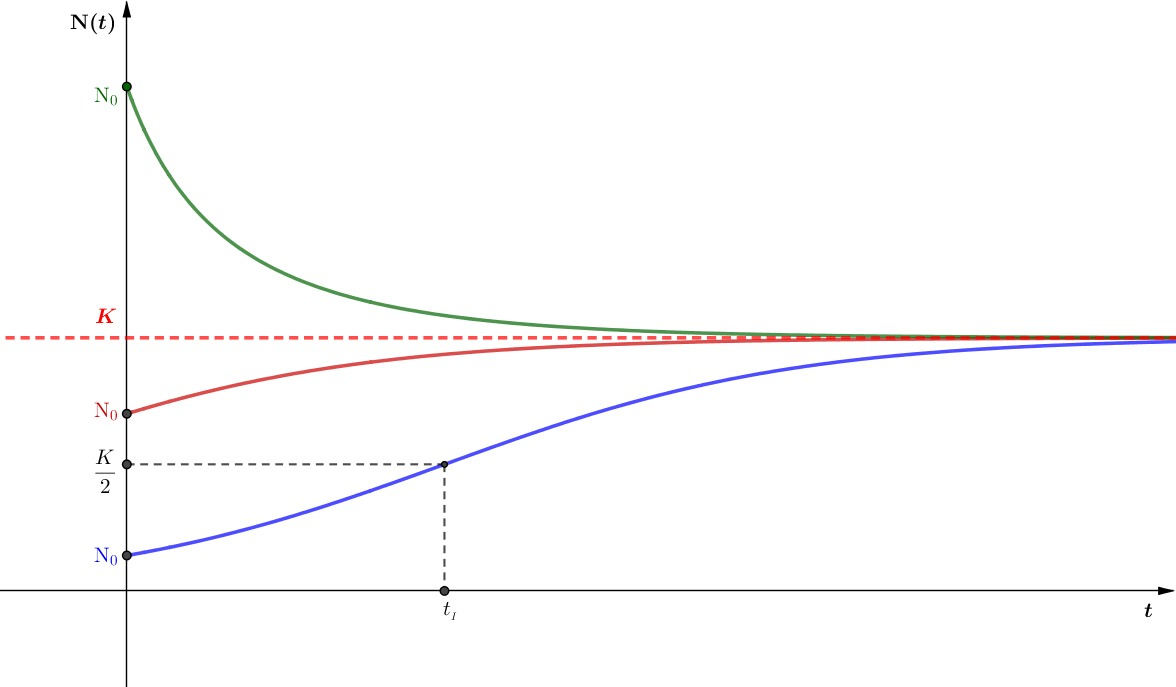
\includegraphics[height=8.cm,width=13.0cm]{figs/verhulst.jpeg}
\fonte{Figura elaborada pelo autor}
\end{center}



Quando \(0 < N_0 < \dfrac{K}{2}\), observa-se que existe um crescimento rápido da população até o tempo \(t_I = \dfrac{-1}{rc} \log\left(\dfrac{K}{N_0}-1\right)\) e depois deste, o crescimento torna-se mais lento.

Quando \(\dfrac{K}{2} < N_0 < K\), observa-se que a população apresenta, apenas, crescimento mais lento.

Quando \(N_0 > K\), observa-se que o número de indivíduos da população, para se ajustar à capacidade de suporte do meio (razão entre o que é produzido e a taxa de consumo \textit{per capita}), deve diminuir.

Em qualquer um dos casos, temos que o número de indivíduos da população tende a capacidade suporte do meio.




%\includepdf[pages=-]{Bio I/pdf/Sol prova 02}
%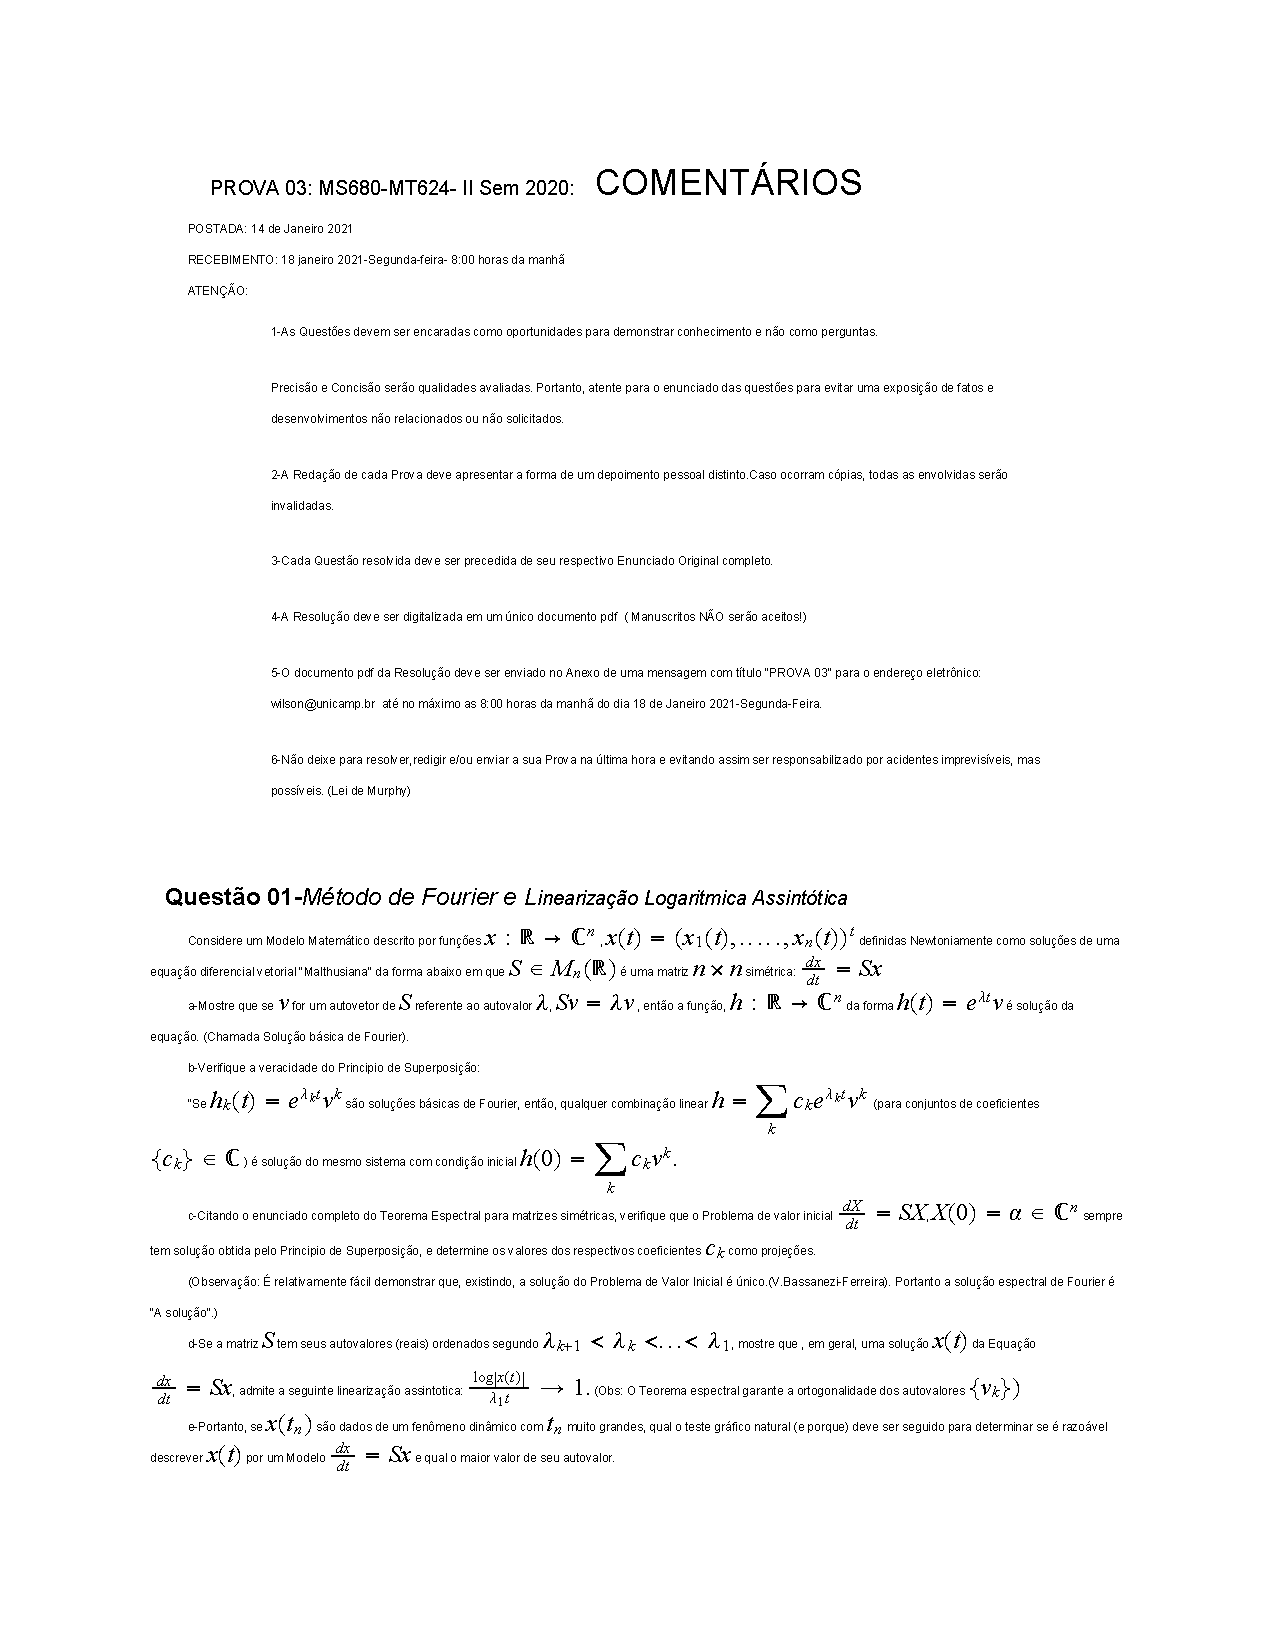
\includepdf[pages=-]{Bio I/pdf/Comentarios_prova03}

%%inserindo apenas uma página
%\includepdf[pages=1,landscape]{V/certificadoRNCINEP2018.pdf}

%%inserindo algumas páginas: 1 até 7, depois 50 e 57
%\includepdf[pages={1-7,50,57}]{arquivo02.pdf}

%%inserindo uma página em branco depois da página 1
%%\includepdf[pages={1,{},2-10}]{arquivo03.pdf}

%%inserindo todas as páginas
%%\includepdf[pages=-]{arquivo04.pdf}

%%inserindo múltiplas páginas numa única página
%%\includepdf[pages={286-291},nup=2x3]{arquivo05.pdf}

%%inserindo páginas em landscape
%%\includepdf[pages=-,landscape]{arquivo06.pdf}

\newpage
%\bibliographystyle{plain}
\bibliography{biblist}

\end{sansmath}
\end{document}